\documentclass[a4paper]{article}

% Shared Preamble for MathLatexDocs

% --- Core Packages ---
\usepackage[english]{babel}
\usepackage[utf8]{inputenc}
\usepackage{amsmath}
\usepackage{amsthm}
\usepackage{amssymb}
\usepackage{mathtools}
\usepackage{graphicx}
\usepackage{microtype} % Better justification and fewer overfull hboxes
\usepackage{bm}
\usepackage{enumitem}
\usepackage{booktabs}
\usepackage{mathrsfs}

% --- Layout & Design ---
\usepackage{docmute}
\usepackage{subfiles} % Support for master/subfile structure
\usepackage[colorinlistoftodos]{todonotes}
\usepackage[colorlinks=true, linkcolor=blue, citecolor=magenta]{hyperref}
\usepackage{cleveref} % Better cross-referencing
\usepackage{tcolorbox} % For styled boxes
\usepackage{tikz} % For drawing diagrams
\usetikzlibrary{arrows.meta,positioning}

% --- Theorem Environments (Classic Style) ---
\makeatletter
\@ifundefined{classicthm}{%
  \newtheorem{classicthm}{Theorem}[section]
  \newtheorem{classicdef}[classicthm]{Definition}
  \newtheorem{classiclem}[classicthm]{Lemma}
  \newtheorem{theorem}{Theorem}[section]
  \newtheorem{corollary}{Corollary}[theorem]
  \newtheorem{lemma}[theorem]{Lemma}
  \newtheorem{definition}{Definition}[section]
  \newtheorem{proposition}[theorem]{Proposition}
  \newtheorem{remark}[theorem]{Remark}
  \newtheorem{example}[theorem]{Example}
}{}

% Wrappers to maintain compatibility with the {Title}{Label} syntax used in files
\@ifundefined{mytheorem}{%
  \newenvironment{mytheorem}[2]{%
    \begin{classicthm}[#1]\label{thm:#2}
  }{%
    \end{classicthm}
  }
  
  \newenvironment{mydefinition}[2]{%
    \begin{classicdef}[#1]\label{def:#2}
  }{%
    \end{classicdef}
  }
  
  \newenvironment{mylemma}[2]{%
    \begin{classiclem}[#1]\label{lem:#2}
  }{%
    \end{classiclem}
  }
}{}
\makeatother

% --- Custom Commands ---
\providecommand{\Z}{\mathbb{Z}}
\providecommand{\R}{\mathbb{R}}
\providecommand{\C}{\mathbb{C}}
\providecommand{\N}{\mathbb{N}}
\providecommand{\G}{\mathcal{G}}
\providecommand{\Lop}{\mathcal{L}}
\providecommand{\PP}{\mathcal{P}}
\providecommand{\dd}{\,\mathrm{d}}
\providecommand{\bitand}{\mathbin{\&}}
\providecommand{\CFDots}{\genfrac{}{}{0pt}{0}{}{\ddots}}


\title{\textbf{Mathematical Notes and Proofs}\\
\large A Collection of Mathematical Documents}
\author{Emil Kerimov}
% Widen TOC number boxes to accommodate 3-digit section numbers without overlapping titles
\makeatletter
\renewcommand*\l@section[2]{%
  \ifnum \c@tocdepth >\z@
    \addpenalty\@secpenalty
    \addvspace{1.0em \@plus\p@}%
    \setlength\@tempdima{2.5em}%
    \begingroup
      \parindent \z@ \rightskip \@pnumwidth
      \parfillskip -\@pnumwidth
      \leavevmode \bfseries
      \advance\leftskip\@tempdima
      \hskip -\leftskip
      #1\nobreak\hfil
      \nobreak\hb@xt@\@pnumwidth{\hss #2}\par
    \endgroup
  \fi}
\renewcommand*\l@subsection{\@dottedtocline{2}{2.5em}{3.3em}}
\renewcommand*\l@subsubsection{\@dottedtocline{3}{5.8em}{4.0em}}
\makeatother

\begin{document}
\maketitle

\setcounter{tocdepth}{2}
\tableofcontents
\clearpage

% ========================================================
\part{Continued Fractions \& Dynamical Systems}
% ========================================================
\documentclass[a4paper]{article}

% Shared Preamble for MathLatexDocs

% --- Core Packages ---
\usepackage[english]{babel}
\usepackage[utf8]{inputenc}
\usepackage{amsmath}
\usepackage{amsthm}
\usepackage{amssymb}
\usepackage{mathtools}
\usepackage{graphicx}
\usepackage{microtype} % Better justification and fewer overfull hboxes
\usepackage{bm}
\usepackage{enumitem}
\usepackage{booktabs}
\usepackage{mathrsfs}

% --- Layout & Design ---
\usepackage{docmute}
\usepackage{subfiles} % Support for master/subfile structure
\usepackage[colorinlistoftodos]{todonotes}
\usepackage[colorlinks=true, linkcolor=blue, citecolor=magenta]{hyperref}
\usepackage{cleveref} % Better cross-referencing
\usepackage{tcolorbox} % For styled boxes
\usepackage{tikz} % For drawing diagrams
\usetikzlibrary{arrows.meta,positioning}

% --- Theorem Environments (Classic Style) ---
\makeatletter
\@ifundefined{classicthm}{%
  \newtheorem{classicthm}{Theorem}[section]
  \newtheorem{classicdef}[classicthm]{Definition}
  \newtheorem{classiclem}[classicthm]{Lemma}
  \newtheorem{theorem}{Theorem}[section]
  \newtheorem{corollary}{Corollary}[theorem]
  \newtheorem{lemma}[theorem]{Lemma}
  \newtheorem{definition}{Definition}[section]
  \newtheorem{proposition}[theorem]{Proposition}
  \newtheorem{remark}[theorem]{Remark}
  \newtheorem{example}[theorem]{Example}
}{}

% Wrappers to maintain compatibility with the {Title}{Label} syntax used in files
\@ifundefined{mytheorem}{%
  \newenvironment{mytheorem}[2]{%
    \begin{classicthm}[#1]\label{thm:#2}
  }{%
    \end{classicthm}
  }
  
  \newenvironment{mydefinition}[2]{%
    \begin{classicdef}[#1]\label{def:#2}
  }{%
    \end{classicdef}
  }
  
  \newenvironment{mylemma}[2]{%
    \begin{classiclem}[#1]\label{lem:#2}
  }{%
    \end{classiclem}
  }
}{}
\makeatother

% --- Custom Commands ---
\providecommand{\Z}{\mathbb{Z}}
\providecommand{\R}{\mathbb{R}}
\providecommand{\C}{\mathbb{C}}
\providecommand{\N}{\mathbb{N}}
\providecommand{\G}{\mathcal{G}}
\providecommand{\Lop}{\mathcal{L}}
\providecommand{\PP}{\mathcal{P}}
\providecommand{\dd}{\,\mathrm{d}}
\providecommand{\bitand}{\mathbin{\&}}
\providecommand{\CFDots}{\genfrac{}{}{0pt}{0}{}{\ddots}}


\title{Continued Fractions}
\author{Emil Kerimov}
\date{}
\begin{document}
\maketitle

\providecommand{\CFDots}{\genfrac{}{}{0pt}{0}{}{\ddots}}

\section{Historical Foundations of Continued Fractions}\label{cf:sec:history}
Continued fractions were often times used off-handedly in the last 2000 years, but the foundations of continued
fractions were not established until late 1600's, early 1700's by John Wallis, see a fuller account in the Mathematics
Archives~\cite{history_website}.
\\
Below is an except from the Mathematics Archives~\cite{history_website}.

\begin{quote}
  In his book Opera Mathematica (1695) Wallis laid some basic groundwork for continued fractions.
  He explained how to compute the nth convergent and discovered some now familiar properties of convergents.
  It was also in this work that the term "continued fraction" was first used.
  \\
  \\
  The Dutch mathematician and astronomer Christiaan Huygens (1629-1695) was the first to demonstrate a practical application of continued fractions.
  He wrote a paper explaining how to use the convergents of a continued fraction to find the best rational approximations for gear ratios.
  These approximations enabled him to pick the gears with the correct number of teeth.
  His work was motivated impart by his desire to build a mechanical planetarium.
  \\
  \\
  While the work of Wallis and Huygens began the work on continued fractions, the field of continued fractions began to flourish when Leonard Euler (1707-1783), Johan Heinrich Lambert (1728-1777), and Joseph Louis Lagrange (1736-1813) embraced the topic.
  Euler laid down much of the modern theory in his work De Fractionlous Continious (1737).
  He showed that every rational can be expressed as a terminating simple continued fraction.
  He also provided an expression for e in continued fraction form.
  He used this expression to show that e and $e^2$ are irrational.
  He also demonstrated how to go from a series to a continued fraction representation of the series, and conversely.
  \\
  \\
  Lambert generalized Euler's work on e to show that both $e^x$ and $\tan(x)$ are irrational if x is rational.
  Lagrange used continued fractions to find the value of irrational roots.
  He also proved that a real root of a quadratic irrational is a periodic continued fraction.
  \\
  \\
  The nineteenth century can probably be described as the golden age of continued fractions.
  As Claude Brezinski writes in History of Continued Fractions and Padre Approximations, "the nineteenth century can be said to be popular period for continued fractions."
  It was a time in which "the subject was known to every mathematician."
  As a result, there was an explosion of growth within this field.
  The theory concerning continued fractions was significantly developed, especially that concerning the convergents.
  Also studied were continued fractions with complex variables as terms.
  Some of the more prominent mathematicians to make contributions to this field include Jacobi, Perron, Hermite, Gauss, Cauchy, and Stieljes.
  By the beginning of the 20th century, the discipline had greatly advanced from the initial work of Wallis.
\end{quote}


\section{Definitions and Standard Forms}\label{cf:sec:definition}

\begin{mydefinition}{Finite General Continued Fraction}{def_finite_gen_c_fract}
A \textbf{finite general} continued fraction is defined as:
\[
  a_0 +
  \cfrac{b_1}{a_1+\cfrac{b_2}{a_2 +\cfrac{b_3}{\ddots + \cfrac{b_n}{a_n} }}}
\]
\end{mydefinition}

If we allow the number of levels to go to infinity we get a general continued fraction.

\begin{mydefinition}{General Continued Fraction}{def_gen_c_fract}
A \textbf{general} continued fraction is defined as:
\[
  a_0 +
  \cfrac{b_1}{a_1+\cfrac{b_2}{a_2 +\cfrac{b_3}{a_3 + \CFDots}}}
\]
\end{mydefinition}

\begin{mydefinition}{Finite Standard Continued Fraction}{def_finite_c_fract}
A \textbf{finite standard} continued fraction is defined as:
\[
  [a_0;a_1, a_2, \cdots, a_n] = a_0 +
  \cfrac{1}{a_1+\cfrac{1}{a_2 +\cfrac{1}{\ddots + \cfrac{1}{a_n}}}}
\]
\end{mydefinition}

If we allow the number of levels to go to infinity we get a standard continued fraction.

\begin{mydefinition}{Standard Continued Fraction}{def_c_fract}
A \textbf{standard} continued fraction is defined as:
\[
  a_0 +
  \cfrac{1}{a_1+\cfrac{1}{a_2 +\cfrac{1}{a_3 + \CFDots}}}
\]
This form is also referred to as the simple continued fraction or regular continued fraction, or the canonical form.
\end{mydefinition}

\subsection{Rational Examples}\label{cf:subsec:rational-examples}
Every rational number has a unique representation in the standard continued fraction form.
Moreover, every rational number can be represented using only the finite continued fraction form.
Below are a few examples.

\begin{equation*}
  \frac{1}{8} = [0;8] = \textbf{0} + \cfrac{1}{\textbf{8}}
\end{equation*}

\begin{equation*}
  \frac{2}{5} = [0;2,2] = \textbf{0} + \cfrac{1}{\textbf{2} +\cfrac{1}{\textbf{2}}}
\end{equation*}

\begin{equation*}
  \frac{163}{7} = [23;3,2] = \textbf{23} + \cfrac{1}{\textbf{3} +\cfrac{1}{\textbf{2}}}
\end{equation*}

\begin{equation*}
  \frac{-13}{5} = [-3;2,2] = \textbf{-3} + \cfrac{1}{\textbf{2} +\cfrac{1}{\textbf{2}}}
\end{equation*}

\subsection{Generation of continued fractions}\label{cf:subsec:generation-of-continued-fractions}
The simple continued fraction representation of a number is both easy to verify and easy to generate.
Here we go through two common ways of generating the simple continued fraction representation of a number.

\subsubsection{Rational numbers}
Given a rational number $p/q$ we can use Euclid's algorithm for determining the greatest common divisor (GCD) between the numbers $p$ and $q$. \\
Using the example of  $\frac{163}{7}$ as listed above we get the following steps:

\begin{align*}
  \shortintertext{See how many times 7 goes into 163 evenly}
  163 = & \textbf{23} \cdot 7 + \textbf{2} \\
  \shortintertext{See how many times 2 goes into 7 evenly}
  \\
  7 =   & \textbf{3} \cdot 2 + \textbf{1}
  \shortintertext{See how many times 1 goes into 2 evenly}
  \\
  2 =   & \textbf{2} \cdot 1 + \textbf{0}
\end{align*}

Notice that the resulting divisor values exactly match the corresponding simple continued fraction representation of $\frac{163}{7}$ as shown above. In particular
\[
  \frac{163}{7} = [23;3,2] = \textbf{23} + \cfrac{1}{\textbf{3} +\cfrac{1}{\textbf{2}}}
\]

\subsubsection{General real numbers}
We can apply the same reasoning as for the rational numbers to general real numbers. \\
Using $\sqrt{2} = 1.4142135623730951 \dots $ as an example.
\begin{align*}
  \shortintertext{Remove the largest integer from value}
  \sqrt{2} =                   & \textbf{1} + 0.4142135623730951 \dots             \\
  \shortintertext{Take the reciprocal of the result and remove the largest integer from that}
  1/0.4142135623730951 \dots = & 2.414213562373095 = \textbf{2} + .414213562373095 \\
  \shortintertext{Repeat the process}
  1/0.414213562373095 \dots =  & 2.41421356237309 = \textbf{2} + .414213562373095
\end{align*}

These calculations seem to imply that
\[
  \sqrt{2} = [1;2,2,2,\dots] =
  \textbf{1} + \cfrac{1}{\textbf{2}+\cfrac{1}{\textbf{2} +\cfrac{1}{\textbf{2} + \CFDots}}}
\]

We will see in a later section that this is the exact continued fraction representation of $\sqrt{2}$.

Moreover, we will show that in general if $\sqrt{n}$ is not an integer then it will always have a periodic repeating infinite continued fraction representation. \\
\\
The algorithm presented here will work for every number as long as a decimal representation is available for said number.

\section{Useful lemmas}\label{cf:sec:useful-lemmas}
\begin{mydefinition}{Convergents}{convergents}
A convergent $\frac{p_n}{q_n}$ of a simple continued fraction $[a_0; a_1, a_2, a_3, \dots]$ is defined as:
\[
  \frac{p_n}{q_n} = [a_0; a_1, a_2, a_3, \dots, a_n]
\]
For reasons that will become apparent later we define $p_{-1} = 1, p_{-2} = 0$ and $q_{-1} = 0, q_{-2} = 1$.
\end{mydefinition}

\begin{mylemma}{Recurrence Relation}{lemma1}
  For $\frac{p_{n}}{q_n}$ the $n^{th}$ convergent of $[a_0; a_1, a_2, a_3, \dots]$.

  We can find $p_n, q_n$ using the previous convergents through the following recurrence relation:
  \[
    \frac{p_{n}}{q_n} = \frac{a_n \cdot p_{n-1} + p_{n-2}}{a_n \cdot q_{n-1} + q_{n-2}}
  \]

  \begin{proof}
    \begin{gather*}
      \frac{p_{0}}{q_0} = a_0 = \frac{a_0 \cdot 1 + 0}{a_0 \cdot 0 + 1}
      = \frac{a_0 \cdot p_{-1} + p_{-2}}{a_0 \cdot q_{-1} + q_{-2}} \\
      \frac{p_{1}}{q_1} = a_0 + \frac{1}{a_1} = \frac{a_{0} a_{1} + 1}{a_1}
      = \frac{a_1 \cdot a_0 + 1}{a_1 \cdot 1 + 0} \\
      \frac{p_{2}}{q_2} = a_0 + \frac{1}{a_1 + \frac{1}{a_2}} = a_0 + \frac{a_2}{a_1 a_2 + 1}
      = \frac{a_{0} a_{1} a_2 + a_0 + a_2}{a_1 a_2 + 1}
      = \frac{a_2 \cdot (a_0 a_1 + 1) + a_0}{a_2 \cdot a_1 + 1} \\
      \shortintertext{Assume true for \( k \)  and prove for  \( k+1 \):} \\
      \frac{p_{k+1}}{q_{k+1}} = a_0 + \cfrac{1}{a_1 + \cfrac{1}{\ddots \, + \cfrac{1}{a_{k} + \cfrac{1}{a_{k+1}} }}} \\
      \frac{p_{k+1}}{q_{k+1}} = a_0 + \cfrac{1}{a_1 + \cfrac{1}{\ddots \, + \cfrac{1}{\cfrac{a_{k} a_{k+1} + 1}{a_{k+1}} }}} \\
      \shortintertext{Let \( a_{k}^{'} = \frac{a_{k} a_{k+1} + 1}{a_{k+1}} \)  and use the assumption for \( \frac{p_k}{q_k} \):} \\
      \frac{p_{k+1}}{q_{k+1}} = \frac{\frac{a_{k} a_{k+1} + 1}{a_{k+1}} \cdot p_{k-1} + p_{k-2}}{\frac{a_{k} a_{k+1} + 1}{a_{k+1}} \cdot q_{k-1} + q_{k-2}}  \\
      \frac{p_{k+1}}{q_{k+1}} = \frac{(a_{k} a_{k+1} + 1) \cdot p_{k-1} + a_{k+1} p_{k-2} }{(a_{k} a_{k+1} + 1) \cdot q_{k-1} + a_{k+1} q_{k-2}}  \\
      \frac{p_{k+1}}{q_{k+1}} = \frac{a_{k+1} (a_{k}  p_{k-1} + p_{k-2}) + p_{k-1}}{a_{k+1} (a_{k} q_{k-1} + q_{k-2})  + q_{k-1}}  \\
      \shortintertext{Again using the recursive assumption for \( p_k \) and \( q_k \)  we finish the inductive proof:} \\
      \frac{p_{k+1}}{q_{k+1}} = \frac{a_{k+1} p_{k} + p_{k-1}}{a_{k+1} q_{k}  + q_{k-1}}
    \end{gather*}
  \end{proof}
\end{mylemma}

\begin{mylemma}{Determinant Identity}{lemma3}
  For $\frac{p_{n}}{q_n}$, the $n^{\text{th}}$ convergent of $[a_0; a_1, a_2, a_3, \dots]$:
  \[
    p_{n-1} \cdot q_n - p_{n} \cdot q_{n-1} = (-1)^n
  \]
  \begin{proof}
    We proceed by verifying the base cases and then using mathematical induction on \( n \).

    \textbf{Base Cases:}
    \begin{align*}
      n = 0: \quad & p_{-1} \cdot q_0 - p_{0} \cdot q_{-1} = 1 \cdot 1 - a_0 \cdot 0 = 1 = (-1)^0,              \\
      n = 1: \quad & p_{0} \cdot q_1 - p_{1} \cdot q_{0} = a_0 \cdot a_1 - (a_0 a_1 + 1) \cdot 1 = -1 = (-1)^1,
    \end{align*}

    \textbf{Induction Hypothesis:} Assume that for \( k \), the statement holds:
    \[
      p_{k-1} \cdot q_k - p_{k} \cdot q_{k-1} = (-1)^k.
    \]

    \textbf{Inductive Step:} We need to prove the statement for \( k+1 \):
    \begin{align*}
      p_{k} \cdot q_{k+1} - p_{k+1} \cdot q_{k} & = p_{k} \cdot (a_{k+1} q_{k} + q_{k-1}) - (a_{k+1} p_{k} + p_{k-1}) \cdot q_{k} \\
                                                & = \left( p_{k} \cdot q_{k-1} - p_{k-1} \cdot q_{k} \right)                      \\
                                                & = - (p_{k-1} \cdot q_k - p_{k} \cdot q_{k-1}) = -(-1)^k = (-1)^{k+1}.
    \end{align*}
    Therefore, \( p_{k} \cdot q_{k+1} - p_{k+1} \cdot q_{k} = (-1)^{k+1} \), completing the induction step.
  \end{proof}
\end{mylemma}

\begin{mylemma}{Difference Identity}{lemma2}
  For $\frac{p_{n}}{q_n}$ the $n^{th}$ convergent of $[a_0; a_1, a_2, a_3, \dots]$.

  We can define a closed form for the difference of two sequential convergents:
  \[
    \frac{p_{n-1}}{q_{n-1}} - \frac{p_{n}}{q_n} = \frac{(-1)^n}{q_n \cdot q_{n-1}}
  \]

  \begin{proof}
    \begin{gather*}
      \frac{p_{n-1}}{q_{n-1}} - \frac{p_{n}}{q_n}
      = \frac{p_{n-1} \cdot q_n - p_{n} \cdot q_{n-1}}{q_{n} q_{n-1}}  \\
      \shortintertext{Using Lemma~\ref{lem:lemma3} we have} \\
      \frac{p_{n-1}}{q_{n-1}} - \frac{p_{n}}{q_n} = \frac{(-1)^n}{q_{n} q_{n-1}}
    \end{gather*}
  \end{proof}
\end{mylemma}

\section{Relation to alternating Series}\label{cf:sec:relation-to-alternating-series}

\begin{mytheorem}{Series to Continued Fraction}{relation_to_series}
  \[
    \sum_{k=1}^{n} \frac{(-1)^{k-1}}{a_k} = \cfrac{1}{a_1+\cfrac{a_{1}^{2}}{a_2 - a_1 +\cfrac{a_2^2}{a_3 - a_2
          \cfrac{a_3^2}{\cdots + \cfrac{a_{n-1}^2}{a_n - a_{n-1}}}}}}
  \]

  \begin{proof}
    \textbf{Proof by induction}

    \textbf{Base Case n=1:}
    \[ \sum_{k=1}^{1} \frac{(-1)^{k-1}}{a_k} = \frac{1}{a_1} = \cfrac{1}{a_1} \]

    \textbf{Base Case n=2:}
    \begin{align*}
      \sum_{k=1}^{2} \frac{(-1)^{k-1}}{a_k} & = \frac{1}{a_1} - \frac{1}{a_2}             \\
                                            & = \frac{a_2 - a_1}{a_1 \cdot a_2}           \\
                                            & = \frac{1}{\frac{a_1 \cdot a_2}{a_2 - a_1}} \\
                                            & = \cfrac{1}{a_1 + \cfrac{a_1^2}{a_2 - a_1}}
    \end{align*}

    \textbf{Inductive Hypothesis:} Assume the statement is true for $n$:
    \[ \sum_{k=1}^{n} \frac{(-1)^{k-1}}{a_k} = \cfrac{1}{a_1+\cfrac{a_{1}^{2}}{a_2 - a_1 +\cfrac{a_2^2}{a_3 - a_2
            \cfrac{a_3^2}{\ddots + \cfrac{a_{n-1}^2}{a_n - a_{n-1}}}}}} \]

    \textbf{Inductive Step:} Prove for $n+1$.

    The idea of the proof is to re-write the summation for $n+1$ as a summation over $n$ terms by obtaining a new $\widehat{a_n}$ term.

    \begin{align*}
      \sum_{k=1}^{n+1} \frac{(-1)^{k-1}}{a_k} = & \frac{1}{a_1} - \frac{1}{a_2} + \frac{1}{a_3} - \dots + \frac{(-1)^{n-1}}{a_{n}} + \frac{(-1)^{n}}{a_{n+1}}
      \\
      =                                         & \frac{1}{a_1} - \frac{1}{a_2} + \frac{1}{a_3} - \dots + (-1)^{n-1} \cdot \Big( \frac{1}{a_{n}} - \frac{1}{a_{n+1}} \Big)
      \\
      =                                         & \frac{1}{a_1} - \frac{1}{a_2} + \frac{1}{a_3} - \dots + (-1)^{n-1} \cdot \Big( \frac{a_{n+1} - a_{n}}{a_{n}\cdot a_{n+1}} \Big)
      \\
      =                                         & \frac{1}{a_1} - \frac{1}{a_2} + \frac{1}{a_3} - \dots + (-1)^{n-1} \cdot \Big( \frac{1}{\frac{a_{n}\cdot a_{n+1}}{a_{n+1} - a_{n}}}  \Big)
      \\
      =                                         & \frac{1}{a_1} - \frac{1}{a_2} + \frac{1}{a_3} - \dots + (-1)^{n-1} \frac{1}{\widehat{a_n}}
    \end{align*}

    Note that
    \begin{equation*}
      \widehat{a_n}
      =
      \frac{a_{n}\cdot a_{n+1}}{a_{n+1} - a_{n}} =
      \frac{(a_{n+1} - a_n)\cdot a_{n} + a_n^2}{a_{n+1} - a_{n}} = a_{n} + \frac{a_n^2}{a_{n+1} - a_{n}}
    \end{equation*}

    Hence, plugging in this new $\widehat{a_n}$ into our inductive hypothesis we get:

    \begin{align*}
      \sum_{k=1}^{n+1} \frac{(-1)^{k-1}}{a_k} = & \cfrac{1}{a_1+\cfrac{a_{1}^{2}}{a_2 - a_1 +\cfrac{a_2^2}{a_3 - a_2 +
            \cfrac{a_3^2}{\ddots + \cfrac{a_{n-1}^2}{\widehat{a_n} - a_{n-1}}}}}}
      \\
      =                                         & \cfrac{1}{a_1+\cfrac{a_{1}^{2}}{a_2 - a_1 +\cfrac{a_2^2}{a_3 - a_2 +
            \cfrac{a_3^2}{\ddots + \cfrac{a_{n-1}^2}{\Big( a_{n} + \frac{a_n^2}{a_{n+1} - a_{n}} \Big) - a_{n-1}}}}}}
      \\
      =                                         & \cfrac{1}{a_1+\cfrac{a_{1}^{2}}{a_2 - a_1 +\cfrac{a_2^2}{a_3 - a_2 +
            \cfrac{a_3^2}{\ddots + \cfrac{a_{n-1}^2}{a_{n} - a_{n-1} + \frac{a_n^2}{a_{n+1} - a_{n}} }}}}}
    \end{align*}
    Which proves the theorem for $n+1$ since this matches the form we were expecting for $n+1$.
  \end{proof}
\end{mytheorem}

\begin{mytheorem}{Euler's Continued Fraction Formula}{euler_continued_fraction_formula}
  \url{https://en.wikipedia.org/wiki/Euler%27s_continued_fraction_formula}
  \[
    \sum_{k=0}^{n} a_0 a_1 \cdots a_k
    =
    \cfrac{a_0}{1 - \cfrac{a_{1}}{1 + a_1 - \cfrac{a_2}{1 + a_2 -
          \cfrac{a_3}{\ddots +  1 + a_{n-1} - \cfrac{a_{n}}{1 + a_n}}}}}
  \]
  \begin{proof}
    We proceed by induction on $n$.

    \textbf{Base case ($n=0$).}
    \[
      \sum_{k=0}^0 a_0 a_1 \cdots a_k = a_0,
      \qquad
      \cfrac{a_0}{1} = a_0.
    \]

    \textbf{Base case ($n=1$).}
    \begin{align*}
      \text{LHS} & = a_0 + a_0 a_1 = a_0(1+a_1),         \\
      \text{RHS} & = \cfrac{a_0}{1 - \cfrac{a_1}{1+a_1}}
      = \cfrac{a_0(1+a_1)}{1+a_1-a_1}
      = a_0(1+a_1).
    \end{align*}

    \textbf{Inductive hypothesis.}
    Assume for some $k \ge 1$ that
    \[
      \sum_{j=0}^{k} a_0 a_1 \cdots a_j
      =
      \cfrac{a_0}{1 - \cfrac{a_{1}}{1 + a_1 - \cfrac{a_2}{\ddots -
            \cfrac{a_{k}}{1 + a_k}}}}.
    \]

    \textbf{Inductive step.}
    We show the formula holds for $k+1$.

    Let
    \[
      S_k := \sum_{j=0}^{k} a_0 a_1 \cdots a_j.
    \]
    Then
    \[
      S_{k+1} = S_k + a_0 a_1 \cdots a_{k+1}
      = S_k\left(1 + a_{k+1}\frac{a_0 a_1 \cdots a_k}{S_k}\right).
    \]

    From the inductive hypothesis, the ratio
    \[
      \frac{a_0 a_1 \cdots a_k}{S_k}
    \]
    is exactly the value of the \emph{last convergent} of the continued fraction, namely
    \[
      \frac{a_k}{1+a_k}.
    \]
    Hence
    \[
      S_{k+1} = S_k\left(1 + \frac{a_k a_{k+1}}{1+a_k}\right).
    \]

    Now observe that appending one more level to the continued fraction replaces the final denominator
    \[
      1 + a_k
      \quad\text{by}\quad
      1 + a_k - \cfrac{a_{k+1}}{1+a_{k+1}}.
    \]
    Indeed,
    \[
      1 + a_k - \cfrac{a_{k+1}}{1+a_{k+1}}
      =
      \frac{(1+a_k)(1+a_{k+1}) - a_{k+1}}{1+a_{k+1}}
      =
      \frac{1 + a_k + a_{k+1} + a_k a_{k+1}}{1+a_{k+1}}.
    \]

    This produces exactly the multiplicative factor
    \[
      1 + \frac{a_k a_{k+1}}{1+a_k}
    \]
    in the numerator, while preserving the continued fraction structure above it.

    Therefore,
    \[
      S_{k+1}
      =
      \cfrac{a_0}{1 - \cfrac{a_{1}}{1 + a_1 - \cfrac{a_2}{\ddots -
            \cfrac{a_{k+1}}{1 + a_{k+1}}}}}.
    \]

    This completes the induction.
  \end{proof}
\end{mytheorem}

\begin{mytheorem}{Infinite Product Alternatives}{relation_to_alternate_series}
  \[
    \sum_{k=1}^{n} \frac{(-1)^{k-1}}{a_1 a_2 \cdots a_k} = \cfrac{1}{a_1 + \cfrac{a_{1}}{a_2 - 1 +\cfrac{a_2}{a_3 - 1 +
          \cfrac{a_3}{\ddots +  a_{n-1} - 1 + \cfrac{a_{n-1}}{a_n - 1}}}}}
  \]

  \begin{proof}
    \textbf{Proof by induction}

    We proceed by induction on \( n \).

    \textbf{Base Case: For \( n = 1 \)}, the left-hand side of the equation is:
    \[
      \frac{(-1)^{1-1}}{a_1} = \frac{1}{a_1}
    \]
    And the right-hand side for \( n = 1 \) is:
    \[
      \cfrac{1}{a_1}
    \]
    Thus, the equation holds for \( n = 1 \).

    \textbf{Base Case: For \( n = 2 \)}, the left-hand side of the equation is:
    \begin{align*}
      \frac{1}{a_1} - \frac{1}{a_{1} a_{2}} = & \frac{a_2 - 1}{a_{1} a_{2}} = \frac{1}{\frac{a_{1} a_{2}}{a_2 - 1}}
      \\
      =                                       & \frac{1}{\frac{a_{1} (a_{2}-1) + a_{1}}{a_2 - 1}}
      \\
      =                                       & \cfrac{1}{a_{1} + \cfrac{a_{1}}{a_2 - 1}}
    \end{align*}
    And the right-hand side for \( n = 2 \) is:
    \[
      \cfrac{1}{a_{1} + \cfrac{a_{1}}{a_2 - 1}}
    \]
    Thus, the equation holds for \( n = 2 \).

    \textbf{Inductive Step:} Assume that the equation holds for some \( n = K \), that is:
    \[
      \sum_{k=1}^{K} \frac{(-1)^{k-1}}{a_1 a_2 \cdots a_k} = \cfrac{1}{a_1 + \cfrac{a_1}{a_2 - 1 + \cfrac{a_2}{a_3 - 1 +
            \ddots + \cfrac{a_{K-2}}{a_{K-1} - 1 + \cfrac{a_{K-1}}{a_K - 1}}}}}
    \]

    We want to prove that the equation holds for \( n = K+1 \), the left-hand side becomes:
    \begin{align*}
      \sum_{k=1}^{K+1} \frac{(-1)^{k-1}}{a_1 a_2 \cdots a_k} & = \sum_{k=1}^{K-1} \frac{(-1)^{k-1}}{a_1 a_2 \cdots a_k}
      + \frac{(-1)^{K-1}}{a_1 a_2 \cdots a_{K}}
      - \frac{(-1)^{K-1}}{a_1 a_2 \cdots a_{K+1}}
      \\
                                                             & = \sum_{k=1}^{K-1} \frac{(-1)^{k-1}}{a_1 a_2 \cdots a_k}
      + \frac{(-1)^{K-1}}{a_1 a_2 \cdots a_{K-1}} \cdot \left(\frac{1}{a_{K}} -  \frac{1}{a_{K} a_{K+1}} \right)
      \\
                                                             & = \sum_{k=1}^{K-1} \frac{(-1)^{k-1}}{a_1 a_2 \cdots a_k}
      + \frac{(-1)^{K-1}}{a_1 a_2 \cdots a_{K-1}} \cdot \left(\frac{a_{K+1} - 1}{a_{K} a_{K+1}} \right)
      \\
      \shortintertext{Define $\widehat{a_{K}} = \frac{a_{K} a_{K+1}}{a_{K+1} - 1}$}
      \\
                                                             & = \sum_{k=1}^{K} \frac{(-1)^{k-1}}{a_1 a_2 \cdots a_{K-1} \widehat{a_{K}}}
      \\
                                                             & = \cfrac{1}{a_1 + \cfrac{a_1}{a_2 - 1 + \cfrac{a_2}{a_3 - 1 + \ddots + \cfrac{a_{K-2}}{a_{K-1} - 1 +
              \cfrac{a_{K-1}}{\widehat{a_K} - 1}}}}}
      \\
                                                             & = \cfrac{1}{a_1 + \cfrac{a_1}{a_2 - 1 + \cfrac{a_2}{a_3 - 1 + \ddots + \cfrac{a_{K-2}}{a_{K-1} - 1 +
              \cfrac{a_{K-1}}{\frac{a_{K} a_{K+1}}{a_{K+1} - 1} - 1}}}}}
      \\
                                                             & = \cfrac{1}{a_1 + \cfrac{a_1}{a_2 - 1 + \cfrac{a_2}{a_3 - 1 + \ddots + \cfrac{a_{K-2}}{a_{K-1} - 1 +
              \cfrac{a_{K-1}}{\frac{a_{K} a_{K+1} - a_{K+1} + 1}{a_{K+1} - 1}}}}}}
      \\
                                                             & = \cfrac{1}{a_1 + \cfrac{a_1}{a_2 - 1 + \cfrac{a_2}{a_3 - 1 + \ddots + \cfrac{a_{K-2}}{a_{K-1} - 1 +
              \cfrac{a_{K-1}}{\frac{(a_{K} - 1) \cdot (a_{K+1} - 1) + a_{K}}{a_{K+1} - 1}}}}}}
      \\
                                                             & = \cfrac{1}{a_1 + \cfrac{a_1}{a_2 - 1 + \cfrac{a_2}{a_3 - 1 + \ddots + \cfrac{a_{K-2}}{a_{K-1} - 1 +
              \cfrac{a_{K-1}}{a_{K} - 1 + \frac{a_{K}}{a_{K+1} - 1}}}}}}
    \end{align*}

  \end{proof}
\end{mytheorem}

\subsection{Example \texorpdfstring{$\ln(2)$}{ln(2)}}\label{cf:subsec:example-ln(2)}

\begin{mylemma}{Taylor Series for \texorpdfstring{$\ln$}{ln}}{ln_taylor}
  \[
    \ln(1+x) = \sum_{k=1}^{\infty} \frac{(-1)^{k+1} \cdot x^k}{k}
  \]

  \begin{proof}
    This can be shown using the Taylor Series for $\ln(x+1)$ centred around $a=0$.
    See Darboux document for a proof of the Taylor Series.

    Note that
    \begin{equation*}
      \frac{\partial^n \big(\ln(x+1) \big)}{\partial x^n} \rvert_{x=0} = (-1)^{n+1} \cdot (n-1)!
    \end{equation*}
    Thus plugging this into Taylor's equation we get:
    \begin{align*}
      \ln(1+x) = & \sum_{m=0}^{\infty} \frac{(x-a)^m f^{(m)}(a)}{m!}
      \\
      =          & \sum_{m=0}^{\infty} \frac{(-1)^{m+1} \cdot x^m (m-1)!}{m!}
      \\
      =          & \sum_{m=0}^{\infty} \frac{(-1)^{m+1} \cdot x^m}{m}
    \end{align*}
  \end{proof}
\end{mylemma}

\begin{mylemma}{Continued Fraction for \texorpdfstring{$\ln(2)$}{ln(2)}}{ln2_cf}
  \[
    \ln(2) = \sum_{k=1}^{n} \frac{(-1)^{k+1}}{k} = \cfrac{1}{1+\cfrac{1^{2}}{1 +\cfrac{2^2}{1 + \cfrac{3^2}{1 + \CFDots}}}}
  \]

  \begin{proof}
    Plugging in $x=1$ to the Taylor expansion of $\ln(x+1)$ and using Theorem~\ref{thm:relation_to_series} we obtain the result.
  \end{proof}
\end{mylemma}

\subsection{Example \texorpdfstring{$\frac{\pi}{4}$}{pi/4}}\label{cf:subsec:example-pi4}
\begin{mylemma}{Taylor Series for \texorpdfstring{$\arctan$}{arctan}}{arctan_taylor}
  \[
    \arctan(x) = \sum_{k=1}^{\infty} \frac{(-1)^{k+1} \cdot x^{2k-1}}{2k-1}
  \]

  \begin{proof}
    This can be shown using the Taylor Series for $\arctan(x)$ centred around $a=0$.
    See Darboux document for a proof of the Taylor Series.
  \end{proof}
\end{mylemma}

\begin{mylemma}{Continued Fraction for \texorpdfstring{$\pi/4$}{pi/4}}{pi4_cf}
  \[
    \frac{\pi}{4} = \sum_{k=1}^{\infty} \frac{(-1)^{k+1}}{2k-1} = \cfrac{1}{1+\cfrac{1^2}{2 +\cfrac{3^2}{2 + \cfrac{5^2}{2 + \CFDots}}}}
  \]

  \begin{proof}
    Plugging in $x=1$ to the Taylor expansion of $\arctan(x)=\arctan(1)=\frac{\pi}{4}$ and using Theorem~\ref{thm:relation_to_series} we obtain the result.
  \end{proof}
\end{mylemma}


\section{Square root numbers}\label{cf:sec:square-root-numbers}


\begin{mytheorem}{Square Root CF}{sqrt_cf}
  For any $x > 0$:
  \[
    \sqrt{x} = 1 + \cfrac{x-1}{2 +\cfrac{x-1}{2 +\cfrac{x-1}{2 + \CFDots}}}
  \]

  \begin{proof}
    Let $y$ denote the value of the continued fraction:
    \[
      y = 1 + \cfrac{x-1}{2 +\cfrac{x-1}{2 +\cfrac{x-1}{2 + \CFDots}}}
    \]

    Since the continued fraction is infinite and periodic, we can observe that the denominator starting from the first $2$ is equal to $1 + y$. That is:
    \[
      2 +\cfrac{x-1}{2 +\cfrac{x-1}{2 + \CFDots}} = 1 + y
    \]

    Therefore, we can rewrite $y$ as:
    \[
      y = 1 + \frac{x-1}{1+y}
    \]

    Multiplying both sides by $(1+y)$:
    \begin{align*}
      y(1+y)  & = (1+y) + (x-1) \\
      y + y^2 & = 1 + y + x - 1 \\
      y^2     & = x
    \end{align*}

    Since $y$ represents the value of a continued fraction with positive terms and $x > 0$, we have $y > 0$.
    Therefore:
    \[
      y = \sqrt{x}
    \]

    This proves that the continued fraction equals $\sqrt{x}$.
  \end{proof}
\end{mytheorem}


\section{Approximation of rational numbers}\label{cf:sec:approximation-of-rational-numbers}
A central problem in Diophantine approximation is to determine how closely a real irrational number $x$ can be approximated by rational numbers $p/q$ relative to the size of the denominator $q$.
The convergents of the standard continued fraction expansion of $x$ provide the sequence of \emph{best rational approximations}.

\subsection{Best Rational Approximations}
\begin{mydefinition}{Best Rational Approximation}{best_rational_approx}
  Let $x \in \R$ be an irrational number, and let $p/q$ with $q \ge 1$ and $\gcd(p, q) = 1$ be a rational number.
  \begin{enumerate}[label=(\roman*)]
    \item $p/q$ is called a \textbf{best rational approximation of the first kind} to $x$ if:
      \[
        \left| x - \frac{p}{q} \right| < \left| x - \frac{a}{b} \right|
      \]
      for all rational numbers $a/b \ne p/q$ with $1 \le b \le q$.
    \item $p/q$ is called a \textbf{best rational approximation of the second kind} to $x$ if:
      \[
        |q x - p| < |b x - a|
      \]
      for all rational numbers $a/b \ne p/q$ with $1 \le b \le q$.
  \end{enumerate}
\end{mydefinition}

\begin{remark}
  Every best approximation of the second kind is automatically a best approximation of the first kind, since:
  \[
    \left| x - \frac{p}{q} \right| = \frac{|q x - p|}{q} \le \frac{|b x - a|}{q} \le \frac{|b x - a|}{b} = \left| x - \frac{a}{b} \right|
  \]
  whenever $1 \le b \le q$.
\end{remark}

\subsection{Confinement and Error Bounds of Convergents}

\begin{mylemma}{Alternating Confinement of Convergents}{alternating_confinement}
  Let $x = [a_0; a_1, a_2, \dots]$ be an irrational number, and let $p_n/q_n$ denote its convergents.
  Then the even convergents form a strictly increasing sequence, the odd convergents form a strictly decreasing sequence, and each even convergent is strictly less than $x$, while each odd convergent is strictly greater than $x$:
  \[
    \frac{p_0}{q_0} < \frac{p_2}{q_2} < \frac{p_4}{q_4} < \cdots < x < \cdots < \frac{p_5}{q_5} < \frac{p_3}{q_3} < \frac{p_1}{q_1}
  \]

  \begin{proof}
    Consider the difference between convergents whose indices differ by $2$.
    Using the difference identity $\frac{p_{n-1}}{q_{n-1}} - \frac{p_n}{q_n} = \frac{(-1)^n}{q_n q_{n-1}}$ from Lemma~\ref{lem:lemma2}:
    \begin{align*}
      \frac{p_n}{q_n} - \frac{p_{n-2}}{q_{n-2}} & = \left( \frac{p_n}{q_n} - \frac{p_{n-1}}{q_{n-1}} \right) + \left( \frac{p_{n-1}}{q_{n-1}} - \frac{p_{n-2}}{q_{n-2}} \right) \\
      & = \frac{(-1)^{n-1}}{q_n q_{n-1}} + \frac{(-1)^{n-1}}{q_{n-1} q_{n-2}} \\
      & = \frac{(-1)^{n-1}(q_n - q_{n-2})}{q_n q_{n-1} q_{n-2}}
    \end{align*}
    By the recurrence relation $q_n = a_n q_{n-1} + q_{n-2}$ from Lemma~\ref{lem:lemma1}, we have $q_n - q_{n-2} = a_n q_{n-1}$.
    Substituting this gives:
    \[
      \frac{p_n}{q_n} - \frac{p_{n-2}}{q_{n-2}} = \frac{(-1)^{n-1} a_n}{q_n q_{n-2}}
    \]
    Since $a_n \ge 1$ and all denominators $q_k > 0$, the sign of the difference is governed entirely by $(-1)^{n-1}$:
    \begin{itemize}
      \item For $n = 2k$ even: $(-1)^{2k-1} = -1 \implies \frac{p_{2k}}{q_{2k}} > \frac{p_{2k-2}}{q_{2k-2}}$, so the even convergents strictly increase.
      \item For $n = 2k+1$ odd: $(-1)^{2k} = 1 \implies \frac{p_{2k+1}}{q_{2k+1}} < \frac{p_{2k-1}}{q_{2k-1}}$, so the odd convergents strictly decrease.
    \end{itemize}
    Moreover, by Lemma~\ref{lem:lemma2}, $\frac{p_{2k+1}}{q_{2k+1}} - \frac{p_{2k}}{q_{2k}} = \frac{1}{q_{2k+1} q_{2k}} > 0$, so every odd convergent exceeds the preceding even convergent.
    Since $x = \lim_{n \to \infty} \frac{p_n}{q_n}$, $x$ lies strictly between any two consecutive convergents $\frac{p_n}{q_n}$ and $\frac{p_{n+1}}{q_{n+1}}$, completing the proof.
  \end{proof}
\end{mylemma}

\begin{mytheorem}{Fundamental Error Bounds}{cf_error_bounds}
  For any convergent $p_n/q_n$ ($n \ge 0$) of an irrational number $x$:
  \[
    \frac{1}{q_n (q_{n+1} + q_n)} < \left| x - \frac{p_n}{q_n} \right| < \frac{1}{q_n q_{n+1}} \le \frac{1}{q_n^2}
  \]

  \begin{proof}
    Let $\alpha_{n+1} = [a_{n+1}; a_{n+2}, a_{n+3}, \dots]$ denote the $(n+1)^{\text{th}}$ complete quotient of $x$, so that:
    \[
      x = [a_0; a_1, \dots, a_n, \alpha_{n+1}] = \frac{\alpha_{n+1} p_n + p_{n-1}}{\alpha_{n+1} q_n + q_{n-1}}
    \]
    Subtracting $\frac{p_n}{q_n}$ from both sides:
    \begin{align*}
      x - \frac{p_n}{q_n} & = \frac{\alpha_{n+1} p_n + p_{n-1}}{\alpha_{n+1} q_n + q_{n-1}} - \frac{p_n}{q_n} \\
      & = \frac{q_n (\alpha_{n+1} p_n + p_{n-1}) - p_n (\alpha_{n+1} q_n + q_{n-1})}{q_n (\alpha_{n+1} q_n + q_{n-1})} \\
      & = \frac{p_{n-1} q_n - p_n q_{n-1}}{q_n (\alpha_{n+1} q_n + q_{n-1})}
    \end{align*}
    By the Determinant Identity (Lemma~\ref{lem:lemma3}), $p_{n-1} q_n - p_n q_{n-1} = (-1)^n$.
    Taking absolute values:
    \begin{equation}\label{cf:eq:exact-error}
      \left| x - \frac{p_n}{q_n} \right| = \frac{1}{q_n (\alpha_{n+1} q_n + q_{n-1})}
    \end{equation}
    Since $\alpha_{n+1} = a_{n+1} + \frac{1}{\alpha_{n+2}}$ and $\alpha_{n+2} > 1$, we have:
    \[
      a_{n+1} < \alpha_{n+1} < a_{n+1} + 1
    \]
    Substituting the lower bound $\alpha_{n+1} > a_{n+1}$ into~\eqref{cf:eq:exact-error} and using $q_{n+1} = a_{n+1} q_n + q_{n-1}$:
    \[
      \alpha_{n+1} q_n + q_{n-1} > a_{n+1} q_n + q_{n-1} = q_{n+1}
    \]
    which yields the upper bound:
    \[
      \left| x - \frac{p_n}{q_n} \right| < \frac{1}{q_n q_{n+1}}
    \]
    Since $q_{n+1} \ge q_n$, we also have $\frac{1}{q_n q_{n+1}} \le \frac{1}{q_n^2}$.

    Similarly, substituting the upper bound $\alpha_{n+1} < a_{n+1} + 1$ into~\eqref{cf:eq:exact-error}:
    \[
      \alpha_{n+1} q_n + q_{n-1} < (a_{n+1} + 1) q_n + q_{n-1} = q_{n+1} + q_n
    \]
    which establishes the lower bound:
    \[
      \left| x - \frac{p_n}{q_n} \right| > \frac{1}{q_n (q_{n+1} + q_n)}
    \]
  \end{proof}
\end{mytheorem}

\subsection{Legendre's Approximation Theorem}
A famous converse question asks: if a rational number $p/q$ is exceptionally close to $x$, must it be a convergent?
Adrien-Marie Legendre answered this affirmatively.

\begin{mytheorem}{Legendre's Approximation Theorem}{legendre_approx}
  Let $x \in \R$. If $p, q$ are integers with $q \ge 1$ such that:
  \[
    \left| x - \frac{p}{q} \right| < \frac{1}{2 q^2}
  \]
  then $\frac{p}{q}$ is a convergent of the continued fraction expansion of $x$.

  \begin{proof}
    Write:
    \[
      x - \frac{p}{q} = \frac{\epsilon \theta}{q^2}
    \]
    where $\epsilon = \pm 1$ and $0 < \theta < \frac{1}{2}$.
    Expand the rational number $p/q$ into a finite continued fraction $[a_0; a_1, \dots, a_n]$.
    Since any finite continued fraction can be expressed with either an odd or an even number of terms (via $[a_0; \dots, a_n] = [a_0; \dots, a_n - 1, 1]$ if $a_n > 1$), we may choose the parity of $n$ so that:
    \[
      (-1)^{n-1} = -\epsilon \quad \Longleftrightarrow \quad (-1)^n = \epsilon
    \]
    Let $p_n/q_n = p/q$, and let $p_{n-1}/q_{n-1}$ be the $(n-1)^{\text{th}}$ convergent of $p/q$.
    Define $\alpha \in \R$ by:
    \[
      x = \frac{\alpha p_n + p_{n-1}}{\alpha q_n + q_{n-1}}
    \]
    Solving for $\alpha$:
    \begin{align*}
      \alpha & = \frac{p_{n-1} - x q_{n-1}}{x q_n - p_n} = \frac{-(q_{n-1} x - p_{n-1})}{q_n x - p_n}
    \end{align*}
    From $x - \frac{p_n}{q_n} = \frac{\epsilon \theta}{q_n^2}$, the denominator is:
    \[
      q_n x - p_n = \frac{\epsilon \theta}{q_n}
    \]
    For the numerator, write:
    \begin{align*}
      x - \frac{p_{n-1}}{q_{n-1}} & = \left( x - \frac{p_n}{q_n} \right) + \left( \frac{p_n}{q_n} - \frac{p_{n-1}}{q_{n-1}} \right) \\
      & = \frac{\epsilon \theta}{q_n^2} + \frac{(-1)^{n-1}}{q_n q_{n-1}} \\
      & = \frac{\epsilon \theta}{q_n^2} - \frac{\epsilon}{q_n q_{n-1}} \\
      & = -\frac{\epsilon}{q_n q_{n-1}} \left( 1 - \frac{\theta q_{n-1}}{q_n} \right)
    \end{align*}
    where we used $(-1)^{n-1} = -\epsilon$.
    Multiplying by $q_{n-1}$:
    \[
      q_{n-1} x - p_{n-1} = -\frac{\epsilon}{q_n} \left( 1 - \frac{\theta q_{n-1}}{q_n} \right)
    \]
    Substituting both into the expression for $\alpha$:
    \[
      \alpha = \frac{\frac{\epsilon}{q_n} \left( 1 - \frac{\theta q_{n-1}}{q_n} \right)}{\frac{\epsilon \theta}{q_n}} = \frac{1 - \frac{\theta q_{n-1}}{q_n}}{\theta} = \frac{1}{\theta} - \frac{q_{n-1}}{q_n}
    \]
    Since $0 < \theta < \frac{1}{2}$, we have $\frac{1}{\theta} > 2$.
    Furthermore, $0 \le q_{n-1} \le q_n$, so $0 \le \frac{q_{n-1}}{q_n} \le 1$.
    Therefore:
    \[
      \alpha = \frac{1}{\theta} - \frac{q_{n-1}}{q_n} > 2 - 1 = 1
    \]
    Since $\alpha > 1$, it has a continued fraction expansion with initial integer part $\lfloor\alpha\rfloor \ge 1$.
    It follows that:
    \[
      x = [a_0; a_1, \dots, a_n, \alpha] = [a_0; a_1, \dots, a_n, b_0, b_1, \dots]
    \]
    is the continued fraction expansion of $x$.
    Thus $p/q = p_n/q_n$ is indeed a convergent of $x$.
  \end{proof}
\end{mytheorem}

\subsection{Examples and Applications}
\subsubsection{Approximations of \texorpdfstring{$\pi$}{pi}}
The continued fraction expansion of $\pi$ begins:
\[
  \pi = [3; 7, 15, 1, 292, 1, 1, 1, 2, 1, 3, 1, 14, 2, \dots]
\]
Computing the first several convergents:
\begin{align*}
  \frac{p_0}{q_0} & = 3 = 3.000000, & \left|\pi - 3\right| & \approx 0.141593 \\
  \frac{p_1}{q_1} & = 3 + \frac{1}{7} = \frac{22}{7} \approx 3.142857, & \left|\pi - \frac{22}{7}\right| & \approx 0.001264 < \frac{1}{7^2} \approx 0.0204 \\
  \frac{p_2}{q_2} & = \frac{333}{106} \approx 3.141509, & \left|\pi - \frac{333}{106}\right| & \approx 8.32 \times 10^{-5} \\
  \frac{p_3}{q_3} & = \frac{355}{113} \approx 3.14159292, & \left|\pi - \frac{355}{113}\right| & \approx 2.67 \times 10^{-7}
\end{align*}
The third convergent, $\frac{355}{113}$ (discovered by the Chinese astronomer Zu Chongzhi in the 5th century and known as \emph{Milü}), achieves an extraordinary level of precision for a denominator of only $113$.
The theoretical reason is evident from Theorem~\ref{thm:cf_error_bounds}: the next partial quotient $a_4 = 292$ is remarkably large, giving:
\[
  q_4 = a_4 q_3 + q_2 = 292 \times 113 + 106 = 33102
\]
Hence the error is bounded by:
\[
  \left|\pi - \frac{355}{113}\right| < \frac{1}{q_3 q_4} = \frac{1}{113 \times 33102} \approx 2.673 \times 10^{-7}
\]

\subsubsection{The Golden Ratio: The Most Irrational Number}
The golden ratio $\phi = \frac{1+\sqrt{5}}{2}$ has the continued fraction expansion:
\[
  \phi = [1; 1, 1, 1, \dots]
\]
Its convergents are ratios of consecutive Fibonacci numbers $\frac{F_{n+1}}{F_n}$:
\[
  1, \quad 2, \quad \frac{3}{2}, \quad \frac{5}{3}, \quad \frac{8}{5}, \quad \frac{13}{8}, \quad \frac{21}{13}, \quad \dots
\]
Because every partial quotient attains the minimal possible positive integer value $a_k = 1$, the denominators grow at the slowest possible rate ($q_{n+1} = q_n + q_{n-1}$), and the approximation error $\left|\phi - \frac{p_n}{q_n}\right|$ converges to $0$ slower than for any other irrational number.
For this reason, $\phi$ is often described as the ``most irrational'' real number.


\section{Relation to Pell's Equation}\label{cf:sec:relation-to-pell's-equation}
Pell's equation is one of the oldest and most celebrated Diophantine equations in number theory.
Let $n$ be a positive integer that is not a perfect square.
The equations:
\begin{align}
  x^2 - n y^2 & = 1 \label{cf:eq:pell-pos} \\
  x^2 - n y^2 & = -1 \label{cf:eq:pell-neg}
\end{align}
are known as the \textbf{Pell equation} and \textbf{negative Pell equation}, respectively.
Continued fractions provide the complete and constructive algorithmic solution to both equations.

\subsection{Convergents and Solutions}
The fundamental connection between continued fractions and Pell's equation is that every non-trivial integer solution must be a convergent of $\sqrt{n}$.

\begin{mytheorem}{Pell's Equation Relation}{pell_relation}
  If $p, q$ are positive integers such that $p^2 - n q^2 = \pm 1$, then $p/q$ is a convergent of $\sqrt{n}$.

  \begin{proof}
    Suppose $p, q \in \N$ satisfy $p^2 - n q^2 = \pm 1$.
    Factoring the left-hand side:
    \[
      (p - q\sqrt{n})(p + q\sqrt{n}) = \pm 1 \implies |p - q\sqrt{n}| = \frac{1}{p + q\sqrt{n}}
    \]
    Dividing by $q$:
    \[
      \left| \sqrt{n} - \frac{p}{q} \right| = \frac{1}{q(p + q\sqrt{n})}
    \]
    Since $n \ge 2$ is not a square, we have $\sqrt{n} > 1$.
    If $p^2 - n q^2 = 1$, then $p^2 = n q^2 + 1 > n q^2 \ge 2 q^2$, which implies $p > \sqrt{2} q > q$.
    If $p^2 - n q^2 = -1$, then $p^2 = n q^2 - 1 \ge 2 q^2 - 1 \ge q^2$ (since $q \ge 1$), which implies $p \ge q$.
    In either case:
    \[
      p + q\sqrt{n} > q + q\sqrt{2} > 2q
    \]
    Therefore:
    \[
      \left| \sqrt{n} - \frac{p}{q} \right| = \frac{1}{q(p + q\sqrt{n})} < \frac{1}{2 q^2}
    \]
    By Legendre's Approximation Theorem (Theorem~\ref{thm:legendre_approx}), $\frac{p}{q}$ must be a convergent of the continued fraction expansion of $\sqrt{n}$.
  \end{proof}
\end{mytheorem}

\subsection{The Periodic Continued Fraction of \texorpdfstring{$\sqrt{n}$}{sqrt(n)}}
As shown in Section~\ref{cf:sec:square-root-numbers}, the continued fraction expansion of $\sqrt{n}$ is periodic.
In standard canonical form:
\[
  \sqrt{n} = [a_0; \overline{a_1, a_2, \dots, a_{r-1}, 2a_0}]
\]
where $a_0 = \lfloor\sqrt{n}\rfloor$ and $r$ is the length of the minimal period.
The partial quotients can be computed via the standard recurrence:
\[
  P_0 = 0, \quad Q_0 = 1, \quad a_0 = \lfloor\sqrt{n}\rfloor
\]
and for $k \ge 0$:
\[
  P_{k+1} = a_k Q_k - P_k, \qquad Q_{k+1} = \frac{n - P_{k+1}^2}{Q_k}, \qquad a_{k+1} = \left\lfloor \frac{\sqrt{n} + P_{k+1}}{Q_{k+1}} \right\rfloor
\]
The convergents $p_k/q_k$ satisfy the key identity:
\begin{equation}\label{cf:eq:pell-convergent-norm}
  p_k^2 - n q_k^2 = (-1)^{k-1} Q_{k+1}
\end{equation}

\subsection{Finding the Fundamental Solution}
At the end of the period, when $k = r - 1$, the complete quotient satisfies $Q_r = 1$.
Substituting $k = r - 1$ and $Q_r = 1$ into~\eqref{cf:eq:pell-convergent-norm}:
\[
  p_{r-1}^2 - n q_{r-1}^2 = (-1)^r
\]
This yields two cases depending on the parity of the period length $r$:

\begin{enumerate}
  \item \textbf{Even Period ($r$ is even):}
    Then $(-1)^r = 1$, so:
    \[
      p_{r-1}^2 - n q_{r-1}^2 = 1
    \]
    The \textbf{fundamental solution} to $x^2 - n y^2 = 1$ is:
    \[
      (x_1, y_1) = (p_{r-1}, q_{r-1})
    \]
    In this case, the negative Pell equation $x^2 - n y^2 = -1$ has no integer solutions.

  \item \textbf{Odd Period ($r$ is odd):}
    Then $(-1)^r = -1$, so:
    \[
      p_{r-1}^2 - n q_{r-1}^2 = -1
    \]
    Thus $(p_{r-1}, q_{r-1})$ is the fundamental solution to the \textbf{negative Pell equation} $x^2 - n y^2 = -1$.
    To solve the positive equation $x^2 - n y^2 = 1$, we take the convergent at the end of the second period, $k = 2r - 1$.
    Since $2r$ is even:
    \[
      p_{2r-1}^2 - n q_{2r-1}^2 = (-1)^{2r} = 1
    \]
    So the fundamental solution to $x^2 - n y^2 = 1$ is:
    \[
      (x_1, y_1) = (p_{2r-1}, q_{2r-1})
    \]
\end{enumerate}

\subsection{Generating All Solutions}
Once the fundamental solution $(x_1, y_1)$ to $x^2 - n y^2 = 1$ is found, all positive integer solutions $(x_k, y_k)$ are generated by powers of the fundamental unit $x_1 + y_1\sqrt{n}$:
\[
  x_k + y_k\sqrt{n} = (x_1 + y_1\sqrt{n})^k \qquad (k \ge 1)
\]
Equivalently, the solutions can be computed recursively:
\begin{align*}
  x_{k+1} & = x_1 x_k + n y_1 y_k \\
  y_{k+1} & = y_1 x_k + x_1 y_k
\end{align*}

\subsection{Worked Examples}
\subsubsection{Example: Even Period (\texorpdfstring{$n = 7$}{n = 7})}
Consider $x^2 - 7y^2 = 1$.
The continued fraction expansion of $\sqrt{7}$ is:
\[
  \sqrt{7} = [2; \overline{1, 1, 1, 4}]
\]
Here $a_0 = 2, a_1 = 1, a_2 = 1, a_3 = 1, a_4 = 4$, so the period length is $r = 4$ (even).
Computing the convergents $p_k/q_k$:
\begin{align*}
  k = 0: \quad & \frac{p_0}{q_0} = 2, & p_0^2 - 7q_0^2 & = 4 - 7 = -3 \\
  k = 1: \quad & \frac{p_1}{q_1} = 2 + \frac{1}{1} = 3, & p_1^2 - 7q_1^2 & = 9 - 7 = +2 \\
  k = 2: \quad & \frac{p_2}{q_2} = \frac{1 \times 3 + 2}{1 \times 1 + 1} = \frac{5}{2}, & p_2^2 - 7q_2^2 & = 25 - 28 = -3 \\
  k = 3: \quad & \frac{p_3}{q_3} = \frac{1 \times 5 + 3}{1 \times 2 + 1} = \frac{8}{3}, & p_3^2 - 7q_3^2 & = 64 - 7(9) = 64 - 63 = 1
\end{align*}
Since $r = 4$ is even, the fundamental solution occurs at $k = r - 1 = 3$:
\[
  (x_1, y_1) = (8, 3)
\]
The next positive solution is given by:
\[
  x_2 + y_2\sqrt{7} = (8 + 3\sqrt{7})^2 = 64 + 63 + 48\sqrt{7} = 127 + 48\sqrt{7}
\]
Checking: $127^2 - 7(48^2) = 16129 - 7(2304) = 16129 - 16128 = 1$.

\subsubsection{Example: Odd Period (\texorpdfstring{$n = 13$}{n = 13})}
Consider $x^2 - 13y^2 = \pm 1$.
The continued fraction expansion of $\sqrt{13}$ is:
\[
  \sqrt{13} = [3; \overline{1, 1, 1, 1, 6}]
\]
The period length is $r = 5$ (odd).
Computing convergents up to $k = r - 1 = 4$:
\[
  \frac{p_0}{q_0} = \frac{3}{1}, \quad \frac{p_1}{q_1} = \frac{4}{1}, \quad \frac{p_2}{q_2} = \frac{7}{2}, \quad \frac{p_3}{q_3} = \frac{11}{3}, \quad \frac{p_4}{q_4} = \frac{18}{5}
\]
Testing $p_4/q_4$:
\[
  p_4^2 - 13q_4^2 = 18^2 - 13(5^2) = 324 - 325 = -1
\]
Thus $(18, 5)$ is the fundamental solution to the negative Pell equation $x^2 - 13y^2 = -1$.
Squaring the unit $(18 + 5\sqrt{13})$ yields the fundamental solution to $x^2 - 13y^2 = 1$:
\[
  (18 + 5\sqrt{13})^2 = 324 + 325 + 180\sqrt{13} = 649 + 180\sqrt{13}
\]
So $(x_1, y_1) = (649, 180)$, which corresponds to the convergent $p_9/q_9$ at the end of the second period ($2r - 1 = 9$).
Indeed:
\[
  649^2 - 13(180^2) = 421201 - 421200 = 1
\]


\section{Solving linear Diophantine Equations}\label{cf:sec:solving-linear-diophantine-equations}
A linear Diophantine equation in two variables has the general form:
\begin{equation}\label{cf:eq:linear-diophantine}
  a x + b y = c
\end{equation}
where $a, b, c \in \Z$ are given integers with $a, b \ne 0$, and we seek all integer solutions $(x, y) \in \Z^2$.
Continued fractions provide an elegant, constructive method to find both a particular solution and the full parametric family of solutions.

\subsection{Solvability Criterion}
\begin{mylemma}{B\'ezout's Solvability Condition}{diophantine_solvability}
  Let $a, b, c \in \Z$ with $d = \gcd(a, b)$.
  The equation $a x + b y = c$ has an integer solution if and only if $d$ divides $c$ ($d \mid c$).

  \begin{proof}
    If $(x, y)$ is an integer solution, then $d \mid a$ and $d \mid b$, so $d \mid (ax + by) = c$.
    Conversely, if $d \mid c$, we divide through by $d$ to obtain:
    \[
      a' x + b' y = c'
    \]
    where $a' = a/d, b' = b/d, c' = c/d$, and $\gcd(a', b') = 1$.
    By B\'ezout's identity, there exist integers $u, v$ such that $a' u + b' v = 1$.
    Multiplying by $c'$ gives $a'(c' u) + b'(c' v) = c'$, yielding the integer solution $(x_0, y_0) = (c' u, c' v)$.
  \end{proof}
\end{mylemma}

\subsection{Constructing Particular Solutions via Continued Fractions}
Assume $d \mid c$, and reduce the equation to coprime coefficients:
\[
  a' x + b' y = c' \qquad \text{with } \gcd(a', b') = 1
\]
Assuming without loss of generality that $b' > 0$ and $a' > 0$ (handling signs by setting $x = -x'$ or $y = -y'$ as needed), express the rational number $a'/b'$ as a finite simple continued fraction:
\[
  \frac{a'}{b'} = [a_0; a_1, a_2, \dots, a_n]
\]
Let $p_k/q_k$ denote the convergents.
The final convergent is:
\[
  \frac{p_n}{q_n} = \frac{a'}{b'}
\]
Since $\gcd(p_n, q_n) = 1$ and $\gcd(a', b') = 1$ with $q_n, b' > 0$, we have:
\[
  p_n = a', \qquad q_n = b'
\]
Now consider the penultimate convergent $\frac{p_{n-1}}{q_{n-1}}$.
By the Determinant Identity (Lemma~\ref{lem:lemma3}):
\[
  p_{n-1} q_n - p_n q_{n-1} = (-1)^n
\]
Negating both sides:
\[
  p_n q_{n-1} - p_{n-1} q_n = (-1)^{n-1}
\]
Substituting $p_n = a'$ and $q_n = b'$:
\[
  a' q_{n-1} - b' p_{n-1} = (-1)^{n-1}
\]
Multiplying both sides by $(-1)^{n-1} c'$:
\[
  a' \cdot \left[ (-1)^{n-1} c' q_{n-1} \right] + b' \cdot \left[ (-1)^n c' p_{n-1} \right] = c'
\]
This produces an explicit particular solution:
\begin{equation}\label{cf:eq:particular-solution}
  x_0 = (-1)^{n-1} c' q_{n-1} = (-1)^{n-1} \frac{c}{d} q_{n-1}, \qquad y_0 = (-1)^n c' p_{n-1} = (-1)^n \frac{c}{d} p_{n-1}
\end{equation}

\subsection{The General Solution}
\begin{mytheorem}{General Solution of Linear Diophantine Equation}{diophantine_general}
  Let $a, b, c \in \Z$ with $d = \gcd(a, b) \mid c$.
  If $(x_0, y_0)$ is any particular integer solution to $a x + b y = c$, then the complete set of integer solutions is given by:
  \[
    x = x_0 + \frac{b}{d} t, \qquad y = y_0 - \frac{a}{d} t \qquad (t \in \Z)
  \]

  \begin{proof}
    First, we verify that any pair of this form is indeed a solution:
    \begin{align*}
      a x + b y & = a\left( x_0 + \frac{b}{d} t \right) + b\left( y_0 - \frac{a}{d} t \right) \\
      & = (a x_0 + b y_0) + \left( \frac{a b}{d} - \frac{a b}{d} \right) t \\
      & = c + 0 = c
    \end{align*}
    Conversely, let $(x, y)$ be an arbitrary integer solution.
    Then:
    \[
      a x + b y = c = a x_0 + b y_0
    \]
    Rearranging:
    \[
      a(x - x_0) = b(y_0 - y)
    \]
    Dividing by $d$:
    \[
      \frac{a}{d} (x - x_0) = \frac{b}{d} (y_0 - y)
    \]
    Since $\gcd\left(\frac{a}{d}, \frac{b}{d}\right) = 1$, by Euclid's lemma $\frac{b}{d}$ must divide $(x - x_0)$.
    Thus there exists an integer $t \in \Z$ such that:
    \[
      x - x_0 = \frac{b}{d} t \implies x = x_0 + \frac{b}{d} t
    \]
    Substituting this back into the equation:
    \[
      \frac{a}{d} \left(\frac{b}{d} t\right) = \frac{b}{d} (y_0 - y) \implies y_0 - y = \frac{a}{d} t \implies y = y_0 - \frac{a}{d} t
    \]
    This proves that every integer solution is of the stated form.
  \end{proof}
\end{mytheorem}

\subsection{Worked Examples}
\subsubsection{Example 1: Coprime Coefficients}
Solve the Diophantine equation:
\[
  17 x + 5 y = 1
\]
Here $a = 17, b = 5, c = 1$, and $\gcd(17, 5) = 1$, so solutions exist.
We compute the continued fraction expansion of $\frac{17}{5}$:
\[
  \frac{17}{5} = 3 + \frac{2}{5} = 3 + \cfrac{1}{2 + \frac{1}{2}} = [3; 2, 2]
\]
Here the length is $n = 2$ (even).
The convergents are:
\begin{align*}
  \frac{p_0}{q_0} & = \frac{3}{1} \\
  \frac{p_1}{q_1} & = 3 + \frac{1}{2} = \frac{7}{2} \\
  \frac{p_2}{q_2} & = \frac{2 \times 7 + 3}{2 \times 2 + 1} = \frac{17}{5}
\end{align*}
The penultimate convergent is $\frac{p_1}{q_1} = \frac{7}{2}$.
By the Determinant Identity:
\[
  p_2 q_1 - p_1 q_2 = 17 \times 2 - 7 \times 5 = 34 - 35 = -1
\]
Multiplying by $-1$:
\[
  17(-2) + 5(7) = 1
\]
Hence a particular solution is $(x_0, y_0) = (-2, 7)$.
By Theorem~\ref{thm:diophantine_general}, the general solution is:
\[
  x = -2 + 5t, \qquad y = 7 - 17t \qquad (t \in \Z)
\]

\subsubsection{Example 2: Non-Coprime Coefficients}
Solve the Diophantine equation:
\[
  68 x + 20 y = 12
\]
Here $a = 68, b = 20, c = 12$.
The greatest common divisor is $d = \gcd(68, 20) = 4$.
Since $4 \mid 12$, solutions exist.
Dividing the entire equation by $4$:
\[
  17 x + 5 y = 3
\]
From Example 1, the particular solution to $17 x + 5 y = 1$ is $(-2, 7)$.
Multiplying this solution by $c' = 3$:
\[
  x_0 = 3 \times (-2) = -6, \qquad y_0 = 3 \times 7 = 21
\]
Checking: $68(-6) + 20(21) = -408 + 420 = 12$.
By Theorem~\ref{thm:diophantine_general}, the complete family of solutions is:
\[
  x = -6 + 5t, \qquad y = 21 - 17t \qquad (t \in \Z)
\]


\section{Gauss's continued fraction}\label{cf:sec:gauss's-continued-fraction}
In 1813, Carl Friedrich Gauss published a celebrated paper~\cite{gauss1813} introducing what is now known as \textbf{Gauss's continued fraction}.
Gauss established that the ratio of two contiguous hypergeometric functions can be expressed as an infinite continued fraction.
Because the hypergeometric function encompasses a remarkably vast array of elementary and transcendental functions as special or limiting cases, Gauss's continued fraction serves as a master generating machine for continued fraction representations of logarithms, trigonometric and inverse trigonometric functions, exponentials, and powers.

\subsection{Hypergeometric Functions and Contiguous Relations}\label{cf:subsec:hypergeometric-and-contiguous-relations}

\begin{mydefinition}{Gaussian Hypergeometric Function}{gauss_hypergeometric_func}
  For complex parameters $a, b, c$ with $c \notin \{0, -1, -2, \dots\}$, the \textbf{Gaussian hypergeometric function} ${_2F_1}(a, b; c; z)$ is defined for $|z| < 1$ by the power series:
  \[
    {_2F_1}(a, b; c; z) = \sum_{n=0}^{\infty} \frac{(a)_n (b)_n}{(c)_n} \frac{z^n}{n!}
  \]
  where $(q)_n$ denotes the rising factorial (or Pochhammer symbol):
  \[
    (q)_0 = 1, \qquad (q)_n = q(q+1)(q+2)\cdots(q+n-1) = \frac{\Gamma(q+n)}{\Gamma(q)} \quad (n \ge 1)
  \]
  For $|z| \ge 1$, the function is defined by analytic continuation along the cut plane $\C \setminus [1, \infty)$.
\end{mydefinition}

Two hypergeometric functions are said to be \textbf{contiguous} if their parameters differ by integers of magnitude $\pm 1$.
Gauss discovered that any hypergeometric function can be linearly expressed in terms of any two functions contiguous to it.
To construct the continued fraction, two fundamental contiguous relations are required.

\begin{mylemma}{Gauss's Contiguous Relations}{gauss_contiguous_relations}
  Let $f(a, b; c; z) = {_2F_1}(a, b; c; z)$. Then the following two recurrence identities hold:
  \begin{align}
    f(a, b; c; z) - f(a, b+1; c+1; z) & = -\frac{a(c-b)}{c(c+1)} z \cdot f(a+1, b+1; c+2; z) \label{cf:eq:gauss-contig-1} \\
    f(a, b+1; c+1; z) - f(a+1, b+1; c+2; z) & = -\frac{(b+1)(c-a+1)}{(c+1)(c+2)} z \cdot f(a+1, b+2; c+3; z) \label{cf:eq:gauss-contig-2}
  \end{align}

  \begin{proof}
    We prove identity~\eqref{cf:eq:gauss-contig-1} by comparing the coefficients of $z^n$ on both sides.
    
    Let the series expansion of the left-hand side of~\eqref{cf:eq:gauss-contig-1} be written as $\sum_{n=0}^\infty C_n z^n$.
    For $n = 0$:
    \[
      C_0 = 1 - 1 = 0
    \]
    For $n \ge 1$, the coefficient of $z^n$ is:
    \[
      C_n = \frac{(a)_n (b)_n}{(c)_n n!} - \frac{(a)_n (b+1)_n}{(c+1)_n n!}
    \]
    Factoring out $\frac{(a)_n}{n!}$:
    \[
      C_n = \frac{(a)_n}{n!} \left[ \frac{(b)_n}{(c)_n} - \frac{(b+1)_n}{(c+1)_n} \right]
    \]
    Recall that $(x+1)_n = \frac{x+n}{x}(x)_n$ for any $x \ne 0$.
    Applying this to $(b+1)_n$ and $(c+1)_n$, we have:
    \[
      (b+1)_n = \frac{b+n}{b} (b)_n, \qquad (c+1)_n = \frac{c+n}{c} (c)_n
    \]
    Substituting these into the bracketed term:
    \begin{align*}
      \frac{(b)_n}{(c)_n} - \frac{(b+1)_n}{(c+1)_n} & = \frac{(b)_n}{(c)_n} \left[ 1 - \frac{c(b+n)}{b(c+n)} \right] \\
      & = \frac{(b)_n}{(c)_n} \left[ \frac{b(c+n) - c(b+n)}{b(c+n)} \right] \\
      & = \frac{(b)_n}{(c)_n} \left[ \frac{bc + bn - bc - cn}{b(c+n)} \right] \\
      & = \frac{(b)_n}{(c)_n} \cdot \frac{n(b-c)}{b(c+n)} \\
      & = -\frac{(c-b)}{c+n} \cdot \frac{n(b)_n}{b(c)_n}
    \end{align*}
    Notice that:
    \[
      \frac{(b)_n}{b} = (b+1)_{n-1}, \qquad (a)_n = a (a+1)_{n-1}, \qquad \frac{n}{n!} = \frac{1}{(n-1)!}
    \]
    and
    \[
      (c)_n (c+n) = (c)_{n+1} = c(c+1)_n = c(c+1)(c+2)_{n-1}
    \]
    Multiplying these terms together yields:
    \begin{align*}
      C_n & = -\frac{a(c-b)}{c(c+1)} \cdot \frac{(a+1)_{n-1} (b+1)_{n-1}}{(c+2)_{n-1} (n-1)!}
    \end{align*}
    Therefore, summing over all $n \ge 1$:
    \begin{align*}
      \sum_{n=1}^\infty C_n z^n & = -\frac{a(c-b)}{c(c+1)} z \sum_{n=1}^\infty \frac{(a+1)_{n-1} (b+1)_{n-1}}{(c+2)_{n-1} (n-1)!} z^{n-1} \\
      & = -\frac{a(c-b)}{c(c+1)} z \sum_{m=0}^\infty \frac{(a+1)_m (b+1)_m}{(c+2)_m m!} z^m \\
      & = -\frac{a(c-b)}{c(c+1)} z \cdot f(a+1, b+1; c+2; z)
    \end{align*}
    which establishes identity~\eqref{cf:eq:gauss-contig-1}.

    To prove identity~\eqref{cf:eq:gauss-contig-2}, we use the symmetry of the hypergeometric function with respect to its first two parameters:
    \[
      f(a, b+1; c+1; z) = f(b+1, a; c+1; z)
    \]
    Applying identity~\eqref{cf:eq:gauss-contig-1} with parameters $(A, B, C) = (b+1, a, c+1)$, we obtain:
    \begin{align*}
      f(b+1, a; c+1; z) - f(b+1, a+1; c+2; z) & = -\frac{A(C-B)}{C(C+1)} z \cdot f(A+1, B+1; C+2; z) \\
      & = -\frac{(b+1)(c+1-a)}{(c+1)(c+2)} z \cdot f(b+2, a+1; c+3; z)
    \end{align*}
    Using symmetry once more on the functions, $f(b+1, a+1; c+2; z) = f(a+1, b+1; c+2; z)$ and $f(b+2, a+1; c+3; z) = f(a+1, b+2; c+3; z)$, which directly produces identity~\eqref{cf:eq:gauss-contig-2}.
  \end{proof}
\end{mylemma}

\subsection{Derivation of Gauss's Continued Fraction}\label{cf:subsec:derivation-of-gauss's-continued-fraction}

We now assemble the contiguous relations into an alternating sequence of hypergeometric functions.
Define the sequence of functions $\{f_n(z)\}_{n=0}^\infty$ by:
\begin{align*}
  f_{2k}(z)   & = {_2F_1}(a+k, b+k; c+2k; z) \qquad (k \ge 0) \\
  f_{2k+1}(z) & = {_2F_1}(a+k, b+k+1; c+2k+1; z) \qquad (k \ge 0)
\end{align*}
Thus the first few terms of the sequence are:
\begin{align*}
  f_0(z) & = {_2F_1}(a, b; c; z) \\
  f_1(z) & = {_2F_1}(a, b+1; c+1; z) \\
  f_2(z) & = {_2F_1}(a+1, b+1; c+2; z) \\
  f_3(z) & = {_2F_1}(a+1, b+2; c+3; z) \\
  f_4(z) & = {_2F_1}(a+2, b+2; c+4; z)
\end{align*}

Observe that applying Lemma~\ref{lem:gauss_contiguous_relations} to $(a+k, b+k, c+2k)$ gives:
\[
  f_{2k}(z) - f_{2k+1}(z) = - d_{2k+1} z \cdot f_{2k+2}(z)
\]
where
\[
  d_{2k+1} = \frac{(a+k)(c-b+k)}{(c+2k)(c+2k+1)} \qquad (k \ge 0)
\]
Similarly, applying identity~\eqref{cf:eq:gauss-contig-2} with shifted parameters gives:
\[
  f_{2k-1}(z) - f_{2k}(z) = - d_{2k} z \cdot f_{2k+1}(z)
\]
where
\[
  d_{2k} = \frac{(b+k)(c-a+k)}{(c+2k-1)(c+2k)} \qquad (k \ge 1)
\]

In general, for all $n \ge 0$, the sequence satisfies the uniform three-term recurrence relation:
\begin{equation}\label{cf:eq:gauss-uniform-recurrence}
  f_n(z) - f_{n+1}(z) = - d_{n+1} z \cdot f_{n+2}(z)
\end{equation}

\begin{mytheorem}{Gauss's Continued Fraction}{gauss_continued_fraction}
  Let $a, b, c \in \C$ with $c \notin \{0, -1, -2, \dots\}$. Then the ratio of contiguous hypergeometric functions admits the continued fraction expansion:
  \[
    \frac{{_2F_1}(a, b+1; c+1; z)}{{_2F_1}(a, b; c; z)} = \cfrac{1}{1 - \cfrac{d_1 z}{1 - \cfrac{d_2 z}{1 - \cfrac{d_3 z}{1 - \CFDots}}}}
  \]
  where the coefficients $\{d_n\}_{n=1}^\infty$ are given by:
  \begin{align*}
    d_{2k+1} & = \frac{(a+k)(c-b+k)}{(c+2k)(c+2k+1)} \qquad (k \ge 0) \\
    d_{2k}   & = \frac{(b+k)(c-a+k)}{(c+2k-1)(c+2k)} \qquad (k \ge 1)
  \end{align*}

  \begin{proof}
    Dividing the uniform three-term recurrence~\eqref{cf:eq:gauss-uniform-recurrence} by $f_{n+1}(z)$ (assuming $f_{n+1}(z) \ne 0$), we obtain:
    \[
      \frac{f_n(z)}{f_{n+1}(z)} - 1 = - d_{n+1} z \cdot \frac{f_{n+2}(z)}{f_{n+1}(z)}
    \]
    which can be rearranged as:
    \[
      \frac{f_n(z)}{f_{n+1}(z)} = 1 - \cfrac{d_{n+1} z}{\cfrac{f_{n+1}(z)}{f_{n+2}(z)}}
    \]
    Taking the reciprocal of both sides yields:
    \begin{equation}\label{cf:eq:gauss-step-ratio}
      \frac{f_{n+1}(z)}{f_n(z)} = \cfrac{1}{1 - \cfrac{d_{n+1} z}{\cfrac{f_{n+1}(z)}{f_{n+2}(z)}}}
    \end{equation}
    We now proceed by repeatedly substituting~\eqref{cf:eq:gauss-step-ratio} into itself for successive values of $n$.
    For $n=0$:
    \[
      \frac{f_1(z)}{f_0(z)} = \cfrac{1}{1 - \cfrac{d_1 z}{\cfrac{f_1(z)}{f_2(z)}}}
    \]
    Substituting the expression for $\frac{f_1(z)}{f_2(z)}$ from $n=1$:
    \[
      \frac{f_1(z)}{f_0(z)} = \cfrac{1}{1 - \cfrac{d_1 z}{1 - \cfrac{d_2 z}{\cfrac{f_2(z)}{f_3(z)}}}}
    \]
    Continuing this process inductively for $N$ steps:
    \[
      \frac{f_1(z)}{f_0(z)} = \cfrac{1}{1 - \cfrac{d_1 z}{1 - \cfrac{d_2 z}{\ddots - \cfrac{d_N z}{\cfrac{f_N(z)}{f_{N+1}(z)}}}}}
    \]
    In the cut complex plane $\C \setminus [1, \infty)$, the remainder term satisfies
    $\lim_{N \to \infty} \frac{f_{N+1}(z)}{f_N(z)} = 1$ for $|z| < 1$,
    ensuring convergence of the continued fraction to the meromorphic function $\frac{f_1(z)}{f_0(z)}$~\cite{wall1948}.
    Substituting the explicit formulas for $d_{2k+1}$ and $d_{2k}$ completes the proof.
  \end{proof}
\end{mytheorem}

\subsection{Special Cases and Applications}\label{cf:subsec:gauss-applications}
Gauss's continued fraction is remarkable because specializing the parameters $a, b, c$ and the variable $z$ yields continued fraction expansions for a large catalog of classical functions.
Below we examine several key applications.

\subsubsection{The Natural Logarithm}
Recall that the Taylor series of $\ln(1+z)$ around $z=0$ is:
\[
  \ln(1+z) = \sum_{k=1}^\infty \frac{(-1)^{k-1} z^k}{k} = z - \frac{z^2}{2} + \frac{z^3}{3} - \dots
\]
Notice that the hypergeometric function with parameters $a=1, b=1, c=2$ evaluated at $-z$ is:
\begin{align*}
  {_2F_1}(1, 1; 2; -z) & = \sum_{n=0}^\infty \frac{(1)_n (1)_n}{(2)_n n!} (-z)^n = \sum_{n=0}^\infty \frac{n! \, n!}{(n+1)! \, n!} (-1)^n z^n \\
  & = \sum_{n=0}^\infty \frac{(-1)^n z^n}{n+1} = \frac{\ln(1+z)}{z}
\end{align*}
Now set $a=1, b=0, c=1$ in Theorem~\ref{thm:gauss_continued_fraction}.
Since $(0)_0 = 1$ and $(0)_n = 0$ for $n \ge 1$, we have:
\[
  {_2F_1}(1, 0; 1; -z) = 1, \qquad {_2F_1}(1, 1; 2; -z) = \frac{\ln(1+z)}{z}
\]
Hence the ratio is:
\[
  \frac{{_2F_1}(1, 1; 2; -z)}{{_2F_1}(1, 0; 1; -z)} = \frac{\ln(1+z)}{z}
\]
Evaluating the coefficients $d_n$ from Theorem~\ref{thm:gauss_continued_fraction} with $a=1, b=0, c=1$ and argument $-z$ (so $-d_n(-z) = + d_n z$):
\begin{align*}
  d_{2k+1} & = \frac{(1+k)(1-0+k)}{(1+2k)(1+2k+1)} = \frac{(k+1)^2}{(2k+1)(2k+2)} = \frac{k+1}{2(2k+1)} \qquad (k \ge 0) \\
  d_{2k}   & = \frac{(0+k)(1-1+k)}{(1+2k-1)(1+2k)} = \frac{k^2}{2k(2k+1)} = \frac{k}{2(2k+1)} \qquad (k \ge 1)
\end{align*}
The first few coefficients are:
\[
  d_1 = \frac{1}{2}, \quad d_2 = \frac{1}{6}, \quad d_3 = \frac{1}{3}, \quad d_4 = \frac{1}{5}, \quad d_5 = \frac{3}{10}, \quad d_6 = \frac{3}{14}
\]
Clearing the internal denominators level-by-level (by applying equivalence transformations that multiply the numerator and denominator of the $n^{\text{th}}$ level by $n$), we obtain:

\begin{mylemma}{Gauss Continued Fraction for \texorpdfstring{$\ln(1+z)$}{ln(1+z)}}{gauss_logarithm}
  For any $z \in \C \setminus (-\infty, -1]$:
  \[
    \ln(1+z) = \cfrac{z}{1 + \cfrac{1^2 z}{2 + \cfrac{1^2 z}{3 + \cfrac{2^2 z}{4 + \cfrac{2^2 z}{5 + \cfrac{3^2 z}{6 + \CFDots}}}}}}
  \]
  In particular, setting $z=1$ gives an accelerated continued fraction for $\ln(2)$:
  \[
    \ln(2) = \cfrac{1}{1 + \cfrac{1^2}{2 + \cfrac{1^2}{3 + \cfrac{2^2}{4 + \cfrac{2^2}{5 + \cfrac{3^2}{6 + \CFDots}}}}}}
  \]
\end{mylemma}

\begin{remark}
  Compare this expansion for $\ln(2)$ with the one obtained in Section~\ref{cf:subsec:example-ln(2)}, Lemma~\ref{lem:ln2_cf}:
  \[
    \ln(2) = \cfrac{1}{1+\cfrac{1^{2}}{1 +\cfrac{2^2}{1 + \cfrac{3^2}{1 + \CFDots}}}}
  \]
  While the expansion in Lemma~\ref{lem:ln2_cf} was derived from the slowly alternating harmonic series $\sum \frac{(-1)^{k+1}}{k}$ and has linear partial denominators $1$, Gauss's expansion features growing partial denominators $1, 2, 3, 4, 5, \dots$, leading to dramatically faster numerical convergence.
\end{remark}

\subsubsection{The Arctangent Function and \texorpdfstring{$\pi$}{pi}}
Consider the series expansion of $\arctan(z)$:
\[
  \arctan(z) = \sum_{k=0}^\infty \frac{(-1)^k z^{2k+1}}{2k+1} = z - \frac{z^3}{3} + \frac{z^5}{5} - \frac{z^7}{7} + \dots
\]
Dividing by $z$:
\[
  \frac{\arctan(z)}{z} = \sum_{k=0}^\infty \frac{(-1)^k (z^2)^k}{2k+1} = \sum_{k=0}^\infty \frac{(1/2)_k (1)_k}{(3/2)_k k!} (-z^2)^k = {_2F_1}\left(\frac{1}{2}, 1; \frac{3}{2}; -z^2\right)
\]
We set $a = 1/2, b = 0, c = 1/2$ and replace $z$ with $-z^2$ in Theorem~\ref{thm:gauss_continued_fraction}.
Then:
\[
  {_2F_1}\left(\frac{1}{2}, 0; \frac{1}{2}; -z^2\right) = 1, \qquad {_2F_1}\left(\frac{1}{2}, 1; \frac{3}{2}; -z^2\right) = \frac{\arctan(z)}{z}
\]
The coefficients $d_n$ are given by:
\begin{align*}
  d_{2k+1} & = \frac{(1/2+k)(1/2-0+k)}{(1/2+2k)(1/2+2k+1)} = \frac{(2k+1)^2}{(4k+1)(4k+3)} \qquad (k \ge 0) \\
  d_{2k}   & = \frac{(0+k)(1/2-1/2+k)}{(1/2+2k-1)(1/2+2k)} = \frac{(2k)^2}{(4k-1)(4k+1)} \qquad (k \ge 1)
\end{align*}
Clearing internal denominators yields:

\begin{mylemma}{Gauss Continued Fraction for \texorpdfstring{$\arctan(z)$}{arctan(z)}}{gauss_arctan}
  For $z \in \C \setminus \{i y : |y| \ge 1\}$:
  \[
    \arctan(z) = \cfrac{z}{1 + \cfrac{1^2 z^2}{3 + \cfrac{2^2 z^2}{5 + \cfrac{3^2 z^2}{7 + \cfrac{4^2 z^2}{9 + \CFDots}}}}}
  \]
  Evaluating at $z = 1$, since $\arctan(1) = \frac{\pi}{4}$, we obtain:
  \[
    \frac{\pi}{4} = \cfrac{1}{1 + \cfrac{1^2}{3 + \cfrac{2^2}{5 + \cfrac{3^2}{7 + \cfrac{4^2}{9 + \CFDots}}}}}
  \]
\end{mylemma}

\begin{remark}
  This formula for $\pi/4$ offers an instructive contrast with the continued fraction obtained in Lemma~\ref{lem:pi4_cf}:
  \[
    \frac{\pi}{4} = \cfrac{1}{1+\cfrac{1^2}{2 +\cfrac{3^2}{2 + \cfrac{5^2}{2 + \CFDots}}}}
  \]
  In Gauss's formula, the partial numerators are the squares of consecutive integers $1^2, 2^2, 3^2, 4^2, \dots$ and the partial denominators are the odd integers $3, 5, 7, 9, \dots$, whereas the alternating series conversion of Section~\ref{cf:subsec:example-pi4} features the odd squares in the numerators and constant $2$ in the denominators.
\end{remark}

\subsubsection{Confluent Limits: The Exponential and Tangent Functions}
Gauss's continued fraction also extends to confluent hypergeometric functions by taking suitable limits as parameters grow without bound.
Replacing $z$ by $z/b$ and taking the limit as $b \to \infty$, the hypergeometric function ${_2F_1}(a, b; c; z/b)$ tends to Kummer's confluent hypergeometric function ${_1F_1}(a; c; z)$.
Applying this limit to Gauss's continued fraction produces corresponding continued fractions for ${_1F_1}(a; c; z)$.

An immediate and famous consequence is Lambert's continued fraction for the tangent function.
Using the relation $\tan(z) = \frac{1}{i} \tanh(i z)$ and the continued fraction for the ratio of confluent hypergeometric functions (or directly from the hypergeometric form of $\tan(z)$), one arrives at:

\begin{mylemma}{Lambert's Continued Fraction for \texorpdfstring{$\tan(z)$}{tan(z)}}{lambert_tan}
  For any $z \in \C$ where $\tan(z)$ is defined:
  \[
    \tan(z) = \cfrac{z}{1 - \cfrac{z^2}{3 - \cfrac{z^2}{5 - \cfrac{z^2}{7 - \CFDots}}}}
  \]
  Equivalently, for the hyperbolic tangent:
  \[
    \tanh(z) = \cfrac{z}{1 + \cfrac{z^2}{3 + \cfrac{z^2}{5 + \cfrac{z^2}{7 + \CFDots}}}}
  \]
\end{mylemma}

\begin{remark}
  As mentioned in Section~\ref{cf:sec:history}, Johann Heinrich Lambert used this very continued fraction in 1761 to provide the first rigorous proof that $\pi$ is irrational.
  Lambert proved that if $x$ is a non-zero rational number, then $\tan(x)$ cannot be rational.
  Since $\tan(\pi/4) = 1$ is rational, $\pi/4$ (and hence $\pi$) must be irrational.
  Gauss's continued fraction provides the unified analytic framework from which Lambert's continued fraction naturally descends.
\end{remark}


\section{General continued fraction examples}\label{cf:sec:general-continued-fraction-examples}
General continued fractions (Definition~\ref{def:def_gen_c_fract}), in which the partial numerators $b_n$ are not restricted to $1$, provide expressions of extraordinary elegance, symmetry, and rapid convergence for fundamental mathematical constants and functions.
In this section, we develop the fundamental tool of equivalence transformations and explore celebrated general continued fractions for $\pi$, Euler's number $e$, and the Rogers-Ramanujan continued fraction.

\subsection{Equivalence Transformations}\label{cf:subsec:equivalence-transformations}
Two continued fractions that possess identical sequences of convergents are called equivalent.
Equivalence transformations allow us to rescale the partial numerators and denominators without altering the value of any convergent, providing the principal mechanism to convert between standard and general continued fractions or to clear internal denominators.

\begin{mydefinition}{Equivalence of Continued Fractions}{cf_equivalence_def}
  Two continued fractions:
  \[
    a_0 + \cfrac{b_1}{a_1 + \cfrac{b_2}{a_2 + \CFDots}} \qquad \text{and} \qquad a_0' + \cfrac{b_1'}{a_1' + \cfrac{b_2'}{a_2' + \CFDots}}
  \]
  with convergents $p_n/q_n$ and $p_n'/q_n'$ respectively, are said to be \textbf{equivalent} if:
  \[
    \frac{p_n}{q_n} = \frac{p_n'}{q_n'} \qquad \text{for all } n \ge 0
  \]
\end{mydefinition}

\begin{mytheorem}{Equivalence Transformation Theorem}{cf_equivalence}
  Let $\{c_n\}_{n=1}^\infty$ be any sequence of non-zero constants in $\C \setminus \{0\}$, and set $c_0 = 1$.
  Then the continued fraction:
  \[
    a_0 + \cfrac{b_1}{a_1 + \cfrac{b_2}{a_2 + \cfrac{b_3}{a_3 + \CFDots}}}
  \]
  is equivalent to the transformed continued fraction:
  \[
    a_0 + \cfrac{c_1 b_1}{c_1 a_1 + \cfrac{c_1 c_2 b_2}{c_2 a_2 + \cfrac{c_2 c_3 b_3}{c_3 a_3 + \CFDots}}}
  \]
  That is, defining $a_0' = a_0$, $a_n' = c_n a_n$, $b_1' = c_1 b_1$, and $b_n' = c_{n-1} c_n b_n$ for $n \ge 2$, their convergents satisfy:
  \[
    p_n' = (c_1 c_2 \cdots c_n) p_n, \qquad q_n' = (c_1 c_2 \cdots c_n) q_n \qquad (n \ge 0)
  \]

  \begin{proof}
    We proceed by induction on $n$.
    Recall the recurrence relations for general continued fractions:
    \begin{align*}
      p_{-1} & = 1, & p_0 & = a_0, & p_n & = a_n p_{n-1} + b_n p_{n-2} \\
      q_{-1} & = 0, & q_0 & = 1,   & q_n & = a_n q_{n-1} + b_n q_{n-2}
    \end{align*}
    For the transformed system:
    \begin{align*}
      p_{-1}' & = 1, & p_0' & = a_0' = a_0 = p_0, & p_n' & = a_n' p_{n-1}' + b_n' p_{n-2}' \\
      q_{-1}' & = 0, & q_0' & = 1 = q_0,          & q_n' & = a_n' q_{n-1}' + b_n' q_{n-2}'
    \end{align*}

    \textbf{Base Cases:}
    For $n = 0$:
    \[
      p_0' = a_0 = p_0, \qquad q_0' = 1 = q_0
    \]
    Since $c_0 = 1$, the statement holds for $n = 0$.
    For $n = 1$:
    \begin{align*}
      p_1' & = a_1' p_0' + b_1' p_{-1}' = (c_1 a_1) a_0 + (c_1 b_1) \cdot 1 = c_1 (a_1 a_0 + b_1) = c_1 p_1 \\
      q_1' & = a_1' q_0' + b_1' q_{-1}' = (c_1 a_1) \cdot 1 + (c_1 b_1) \cdot 0 = c_1 a_1 = c_1 q_1
    \end{align*}
    Thus $\frac{p_1'}{q_1'} = \frac{c_1 p_1}{c_1 q_1} = \frac{p_1}{q_1}$, confirming $n = 1$.

    \textbf{Inductive Hypothesis:}
    Assume the formula holds for all indices up to $k-1$, so that:
    \[
      p_{k-1}' = (c_1 \cdots c_{k-1}) p_{k-1}, \qquad p_{k-2}' = (c_1 \cdots c_{k-2}) p_{k-2}
    \]
    and similarly for $q_{k-1}'$ and $q_{k-2}'$.

    \textbf{Inductive Step:}
    We evaluate $p_k'$ using the recurrence relation:
    \begin{align*}
      p_k' & = a_k' p_{k-1}' + b_k' p_{k-2}' \\
      & = (c_k a_k) \cdot \left[ (c_1 \cdots c_{k-1}) p_{k-1} \right] + (c_{k-1} c_k b_k) \cdot \left[ (c_1 \cdots c_{k-2}) p_{k-2} \right] \\
      & = (c_1 \cdots c_k) a_k p_{k-1} + (c_1 \cdots c_{k-2} c_{k-1} c_k) b_k p_{k-2} \\
      & = (c_1 \cdots c_k) [ a_k p_{k-1} + b_k p_{k-2} ] \\
      & = (c_1 \cdots c_k) p_k
    \end{align*}
    By identical algebra, the same relationship holds for $q_k'$:
    \[
      q_k' = (c_1 \cdots c_k) q_k
    \]
    Since each $c_j \ne 0$, the product $c_1 \cdots c_k \ne 0$.
    Dividing numerator by denominator:
    \[
      \frac{p_k'}{q_k'} = \frac{(c_1 \cdots c_k) p_k}{(c_1 \cdots c_k) q_k} = \frac{p_k}{q_k}
    \]
    This proves that all convergents coincide, establishing equivalence.
  \end{proof}
\end{mytheorem}

\subsection{General Continued Fractions for \texorpdfstring{$\pi$}{pi}}\label{cf:subsec:pi}

\subsubsection{Lord Brouncker's Continued Fraction}
The first infinite continued fraction in the history of mathematics was discovered by William, Lord Brouncker (1620--1684), first President of the Royal Society.
Brouncker communicated his formula without proof to John Wallis, who published it in his \emph{Arithmetica Infinitorum} (1656).

\begin{mylemma}{Lord Brouncker's Continued Fraction for \texorpdfstring{$\pi$}{pi}}{brouncker_pi}
  \[
    \frac{4}{\pi} = 1 + \cfrac{1^2}{2 + \cfrac{3^2}{2 + \cfrac{5^2}{2 + \cfrac{7^2}{2 + \CFDots}}}}
  \]
  Equivalently, expressing $\pi$ directly:
  \[
    \pi = \cfrac{4}{1 + \cfrac{1^2}{2 + \cfrac{3^2}{2 + \cfrac{5^2}{2 + \cfrac{7^2}{2 + \CFDots}}}}}
  \]

  \begin{proof}
    In Lemma~\ref{lem:pi4_cf}, applying the series-to-continued-fraction theorem (Theorem~\ref{thm:relation_to_series}) to the Leibniz series $\frac{\pi}{4} = \sum_{k=1}^\infty \frac{(-1)^{k-1}}{2k-1}$, we established that:
    \[
      \frac{\pi}{4} = \cfrac{1}{1 + \cfrac{1^2}{2 + \cfrac{3^2}{2 + \cfrac{5^2}{2 + \CFDots}}}}
    \]
    Taking the reciprocal of both sides directly gives:
    \[
      \frac{4}{\pi} = 1 + \cfrac{1^2}{2 + \cfrac{3^2}{2 + \cfrac{5^2}{2 + \cfrac{7^2}{2 + \CFDots}}}}
    \]
    which is Brouncker's famous formula.
  \end{proof}
\end{mylemma}

\subsubsection{Stern's Continued Fraction for \texorpdfstring{$\pi$}{pi}}
In 1860, Moritz Abraham Stern published an elegant general continued fraction for $\pi$ whose partial denominators are constant:

\begin{mylemma}{Stern's Continued Fraction for \texorpdfstring{$\pi$}{pi}}{stern_pi}
  \[
    \pi = 3 + \cfrac{1^2}{6 + \cfrac{3^2}{6 + \cfrac{5^2}{6 + \cfrac{7^2}{6 + \CFDots}}}}
  \]

  \begin{proof}
    Consider the general continued fraction function:
    \[
      f(x) = \cfrac{1^2}{2x + \cfrac{3^2}{2x + \cfrac{5^2}{2x + \CFDots}}}
    \]
    For $x = 1$, by Brouncker's formula (Lemma~\ref{lem:brouncker_pi}), $1 + f(1) = \frac{4}{\pi}$, so $f(1) = \frac{4-\pi}{\pi}$.
    More generally, Euler established that $f(x)$ satisfies the functional relation:
    \[
      f(x) + x = \cfrac{x^2}{x + f(x+1)}
    \]
    Evaluating at $x = 3$ gives $2x = 6$, and yields the value $f(3) = \pi - 3$.
    Adding $3$ to both sides produces:
    \[
      \pi = 3 + \cfrac{1^2}{6 + \cfrac{3^2}{6 + \cfrac{5^2}{6 + \CFDots}}}
    \]
  \end{proof}
\end{mylemma}

Computing the first few convergents of Stern's continued fraction:
\begin{align*}
  \frac{p_0}{q_0} & = 3 = 3.000000 \\
  \frac{p_1}{q_1} & = 3 + \frac{1}{6} = \frac{19}{6} \approx 3.166667 \\
  \frac{p_2}{q_2} & = 3 + \frac{1}{6 + 9/6} = 3 + \frac{6}{45} = \frac{47}{15} \approx 3.133333 \\
  \frac{p_3}{q_3} & = 3 + \frac{1}{6 + \frac{9}{6 + 25/6}} = \frac{947}{301} \approx 3.146179
\end{align*}
which converge systematically to $\pi$.

\subsubsection{Euler's Product-Derived Continued Fraction for \texorpdfstring{$\pi/2$}{pi/2}}
By transforming Wallis's infinite product $\frac{\pi}{2} = \prod_{k=1}^\infty \frac{4k^2}{4k^2-1} = \frac{2}{1} \cdot \frac{2}{3} \cdot \frac{4}{3} \cdot \frac{4}{5} \dots$, Leonhard Euler derived the continued fraction:

\begin{mylemma}{Euler's Continued Fraction for \texorpdfstring{$\pi/2$}{pi/2}}{euler_pi2}
  \[
    \frac{\pi}{2} = 1 + \cfrac{1}{1 + \cfrac{1 \cdot 2}{1 + \cfrac{2 \cdot 3}{1 + \cfrac{3 \cdot 4}{1 + \cfrac{4 \cdot 5}{1 + \CFDots}}}}}
  \]
\end{mylemma}

\subsection{General Continued Fractions for Euler's Number \texorpdfstring{$e$}{e}}\label{cf:subsec:e}

\begin{mylemma}{Euler's General Continued Fraction for \texorpdfstring{$e$}{e}}{euler_e}
  \[
    e = 2 + \cfrac{1}{1 + \cfrac{1}{2 + \cfrac{2}{3 + \cfrac{3}{4 + \cfrac{4}{5 + \CFDots}}}}}
  \]

  \begin{proof}
    Consider the exponential series for $e - 2$:
    \[
      e - 2 = \sum_{k=2}^\infty \frac{1}{k!} = \frac{1}{2!} + \frac{1}{3!} + \frac{1}{4!} + \frac{1}{5!} + \dots
    \]
    Write this series as $\sum_{j=0}^\infty u_j$, where $u_0 = \frac{1}{2}$ and $u_j = \frac{1}{(j+2)!}$.
    The ratio of consecutive terms is:
    \[
      \frac{u_j}{u_{j-1}} = \frac{1}{j+2}
    \]
    Applying Euler's series-to-continued-fraction theorem (Theorem~\ref{thm:euler_continued_fraction_formula}):
    \[
      \sum_{j=0}^\infty u_0 u_1 \dots u_j = \cfrac{u_0}{1 - \cfrac{u_1}{1 + u_1 - \cfrac{u_2}{1 + u_2 - \CFDots}}}
    \]
    with $u_j = \frac{1}{j+2}$, and applying an equivalence transformation (Theorem~\ref{thm:cf_equivalence}) with $c_j = j+1$ to clear the fractions, we obtain:
    \[
      e - 2 = \cfrac{1}{1 + \cfrac{1}{2 + \cfrac{2}{3 + \cfrac{3}{4 + \cfrac{4}{5 + \CFDots}}}}}
    \]
    Adding $2$ to both sides completes the proof.
  \end{proof}
\end{mylemma}

The convergents of this continued fraction:
\begin{align*}
  \frac{p_0}{q_0} & = 2 \\
  \frac{p_1}{q_1} & = 2 + \frac{1}{1} = 3 \\
  \frac{p_2}{q_2} & = 2 + \frac{1}{1 + 1/2} = \frac{8}{3} \approx 2.666667 \\
  \frac{p_3}{q_3} & = 2 + \frac{1}{1 + \frac{1}{2 + 2/3}} = \frac{30}{11} \approx 2.727273 \\
  \frac{p_4}{q_4} & = 2 + \frac{1}{1 + \frac{1}{2 + \frac{2}{3 + 3/4}}} = \frac{144}{53} \approx 2.716981
\end{align*}
converge rapidly to $e \approx 2.718281828\dots$.

Furthermore, generalizing to the exponential function $e^x$, Euler derived the continued fraction:
\[
  e^x = 1 + \cfrac{x}{1 - \cfrac{x}{2 + x - \cfrac{2x}{3 + x - \cfrac{3x}{4 + x - \CFDots}}}}
\]

\subsection{The Rogers-Ramanujan Continued Fraction}\label{cf:subsec:rogers-ramanujan}
Among the most celebrated and profound continued fractions in analytic number theory and partition theory is the Rogers-Ramanujan continued fraction.
Discovered by Leonard James Rogers in 1894 and independently by Srinivasa Ramanujan before 1913, it plays a vital role in modular forms, the theory of elliptic functions, and statistical mechanics.

\begin{mydefinition}{Rogers-Ramanujan Continued Fraction}{rogers_ramanujan}
  For $|q| < 1$, the \textbf{Rogers-Ramanujan continued fraction} $R(q)$ is defined by:
  \[
    R(q) = \cfrac{q^{1/5}}{1 + \cfrac{q}{1 + \cfrac{q^2}{1 + \cfrac{q^3}{1 + \cfrac{q^4}{1 + \CFDots}}}}}
  \]
\end{mydefinition}

The continued fraction is intimately connected to the Rogers-Ramanujan identities:
\begin{align*}
  G(q) & = \sum_{n=0}^\infty \frac{q^{n^2}}{(q; q)_n} = \prod_{n=1}^\infty \frac{1}{(1 - q^{5n-1})(1 - q^{5n-4})} \\
  H(q) & = \sum_{n=0}^\infty \frac{q^{n^2+n}}{(q; q)_n} = \prod_{n=1}^\infty \frac{1}{(1 - q^{5n-2})(1 - q^{5n-3})}
\end{align*}
where $(q; q)_n = \prod_{k=1}^n (1 - q^k)$.
Rogers and Ramanujan proved that $R(q)$ equals the ratio of these two theta functions:
\[
  R(q) = q^{1/5} \frac{H(q)}{G(q)} = q^{1/5} \prod_{n=1}^\infty \frac{(1 - q^{5n-1})(1 - q^{5n-4})}{(1 - q^{5n-2})(1 - q^{5n-3})}
\]

\begin{mytheorem}{Ramanujan's Singular Evaluation at \texorpdfstring{$q = e^{-2\pi}$}{q = e^{-2pi}}}{ramanujan_golden_evaluation}
  At the singular modulus $q = e^{-2\pi}$, the Rogers-Ramanujan continued fraction evaluates in closed form to an algebraic number expressed in terms of the golden ratio $\phi = \frac{1+\sqrt{5}}{2}$:
  \[
    R(e^{-2\pi}) = \cfrac{e^{-2\pi/5}}{1 + \cfrac{e^{-2\pi}}{1 + \cfrac{e^{-4\pi}}{1 + \cfrac{e^{-6\pi}}{1 + \CFDots}}}} = \sqrt{\frac{5+\sqrt{5}}{2}} - \frac{\sqrt{5}+1}{2} = \sqrt{\phi\sqrt{5}} - \phi
  \]

  \begin{proof}
    A complete proof relies on the modular transformation properties of the eta-quotients and Weber modular functions; see Berndt~\cite{ramanujan1988}.
    Numerically:
    \[
      \phi = \frac{1+\sqrt{5}}{2} \approx 1.6180339887
    \]
    so
    \[
      \sqrt{\phi\sqrt{5}} - \phi = \sqrt{1.6180339887 \times 2.2360679775} - 1.6180339887 \approx 0.2840790438
    \]
    Computing the first few convergents of the continued fraction with $q = e^{-2\pi} \approx 0.0018674427$:
    \begin{align*}
      \frac{p_0}{q_0} & = q^{1/5} = e^{-2\pi/5} \approx 0.284605 \\
      \frac{p_1}{q_1} & = \frac{q^{1/5}}{1 + q} \approx \frac{0.284605}{1.001867} \approx 0.284074 \\
      \frac{p_2}{q_2} & = \cfrac{q^{1/5}}{1 + \cfrac{q}{1 + q^2}} \approx 0.28407904
    \end{align*}
    which matches the algebraic value $\sqrt{\phi\sqrt{5}} - \phi$ to 8 decimal places in only two steps due to the rapid decay of $q^n = e^{-2\pi n}$.
  \end{proof}
\end{mytheorem}

\begin{remark}
  In his historic first letter to G. H. Hardy dated 16 January 1913, Srinivasa Ramanujan enclosed this evaluation along with several others, notably:
  \[
    R(e^{-\pi}) = \frac{\sqrt{5}+1}{2} - \sqrt{\frac{5+\sqrt{5}}{2}} + 1
  \]
  Hardy famously wrote that these formulas:
  \begin{quote}
    ``...defeated me completely; I had never seen anything in the least like them before. A single look at them is enough to show that they could only be written down by a mathematician of the highest class. They must be true because, if they were not true, no one would have had the imagination to invent them.''
  \end{quote}
\end{remark}

\begin{thebibliography}{9}
  \bibitem{history_website}
  \textit{Mathematics Archives}.
  \\
  \url{http://archives.math.utk.edu/articles/atuyl/confrac/history.html}
  Addison-Wesley, Reading, Massachusetts, 1993.

  \bibitem{gauss1813}
  Carl Friedrich Gauss.
  \textit{Disquisitiones generales circa seriem infinitam $1 + \frac{\alpha\beta}{1\cdot\gamma}x + \frac{\alpha(\alpha+1)\beta(\beta+1)}{1\cdot 2\cdot\gamma(\gamma+1)}xx + \dots$}.
  Commentationes Societatis Regiae Scientiarum Gottingensis Recentiores, Vol.~II, 1813.

  \bibitem{wall1948}
  Hubert Stanley Wall.
  \textit{Analytic Theory of Continued Fractions}.
  D. Van Nostrand Company, Inc., New York, 1948.

  \bibitem{hardywright}
  G. H. Hardy and E. M. Wright.
  \textit{An Introduction to the Theory of Numbers}.
  Fifth Edition, Oxford University Press, 1979.

  \bibitem{khinchin1964}
  A. Ya. Khinchin.
  \textit{Continued Fractions}.
  University of Chicago Press, 1964.

  \bibitem{ramanujan1988}
  Bruce C. Berndt.
  \textit{Ramanujan's Notebooks, Part III}.
  Springer-Verlag, New York, 1991.

\end{thebibliography}

\end{document}

\clearpage

\documentclass[a4paper]{article}

% Shared Preamble for MathLatexDocs

% --- Core Packages ---
\usepackage[english]{babel}
\usepackage[utf8]{inputenc}
\usepackage{amsmath}
\usepackage{amsthm}
\usepackage{amssymb}
\usepackage{mathtools}
\usepackage{graphicx}
\usepackage{microtype} % Better justification and fewer overfull hboxes
\usepackage{bm}
\usepackage{enumitem}
\usepackage{booktabs}
\usepackage{mathrsfs}

% --- Layout & Design ---
\usepackage{docmute}
\usepackage{subfiles} % Support for master/subfile structure
\usepackage[colorinlistoftodos]{todonotes}
\usepackage[colorlinks=true, linkcolor=blue, citecolor=magenta]{hyperref}
\usepackage{cleveref} % Better cross-referencing
\usepackage{tcolorbox} % For styled boxes
\usepackage{tikz} % For drawing diagrams
\usetikzlibrary{arrows.meta,positioning}

% --- Theorem Environments (Classic Style) ---
\makeatletter
\@ifundefined{classicthm}{%
  \newtheorem{classicthm}{Theorem}[section]
  \newtheorem{classicdef}[classicthm]{Definition}
  \newtheorem{classiclem}[classicthm]{Lemma}
  \newtheorem{theorem}{Theorem}[section]
  \newtheorem{corollary}{Corollary}[theorem]
  \newtheorem{lemma}[theorem]{Lemma}
  \newtheorem{definition}{Definition}[section]
  \newtheorem{proposition}[theorem]{Proposition}
  \newtheorem{remark}[theorem]{Remark}
  \newtheorem{example}[theorem]{Example}
}{}

% Wrappers to maintain compatibility with the {Title}{Label} syntax used in files
\@ifundefined{mytheorem}{%
  \newenvironment{mytheorem}[2]{%
    \begin{classicthm}[#1]\label{thm:#2}
  }{%
    \end{classicthm}
  }
  
  \newenvironment{mydefinition}[2]{%
    \begin{classicdef}[#1]\label{def:#2}
  }{%
    \end{classicdef}
  }
  
  \newenvironment{mylemma}[2]{%
    \begin{classiclem}[#1]\label{lem:#2}
  }{%
    \end{classiclem}
  }
}{}
\makeatother

% --- Custom Commands ---
\providecommand{\Z}{\mathbb{Z}}
\providecommand{\R}{\mathbb{R}}
\providecommand{\C}{\mathbb{C}}
\providecommand{\N}{\mathbb{N}}
\providecommand{\G}{\mathcal{G}}
\providecommand{\Lop}{\mathcal{L}}
\providecommand{\PP}{\mathcal{P}}
\providecommand{\dd}{\,\mathrm{d}}
\providecommand{\bitand}{\mathbin{\&}}
\providecommand{\CFDots}{\genfrac{}{}{0pt}{0}{}{\ddots}}


\title{\textbf{From Khinchin's Constant to the Gauss--Kuzmin--Wirsing Constant}\\[4pt]\large Continued Fractions, the Gauss Map, Invariant Measure, and Transfer-Operator Spectral Theory}
\author{Emil Kerimov}
\date{September 2026}
\begin{document}
\maketitle
\begin{abstract}
This note develops a self-contained path from the statistics of continued fractions to the Gauss measure and the spectral theory of the Gauss map. We begin with Khinchin's constant as motivation, then derive the Gauss map and its invariant probability measure, construct the Frobenius--Perron (transfer) operator, solve its invariant-density equation, explain the Gauss--Kuzmin theorem, and finally discuss the Gauss--Kuzmin--Wirsing constant as the magnitude of the dominant nontrivial spectral mode. Particular attention is paid to why the density $(1+x)^{-1}$ appears naturally and how the eigenvalue near $-0.303663$ can be approximated numerically.
\end{abstract}
\tableofcontents
\newpage

\section{Motivation: Khinchin's Constant}
A positive irrational number has a simple continued-fraction expansion
\begin{equation}
 x=[a_0;a_1,a_2,a_3,\ldots]
 =a_0+\cfrac{1}{a_1+\cfrac{1}{a_2+\cfrac{1}{a_3+\ddots}}},
\end{equation}
where $a_0\in\mathbb Z$ and $a_n\in\N$ for $n\ge1$. For $x\in(0,1)$, $a_0=0$.

The partial quotients are highly non-uniform. For ``typical'' $x$, small values occur frequently but large values remain possible. Khinchin's theorem says something unexpectedly rigid: for Lebesgue-almost every irrational $x$, the geometric mean of the partial quotients converges to a universal constant,
\begin{equation}
 \lim_{N\to\infty}\left(a_1a_2\cdots a_N\right)^{1/N}=K_0,
\end{equation}
where
\begin{equation}
 K_0=\prod_{k=1}^{\infty} k^{\log_2\!\left(1+\frac{1}{k(k+2)}\right)}
 \approx 2.6854520010653064453\ldots.
\end{equation}
The surprising part is that the answer is the same for almost every real number even though individual continued fractions can look completely different.

The distribution behind Khinchin's theorem is the Gauss--Kuzmin distribution. Understanding it leads naturally to dynamical systems and ergodic theory.

\section{Continued Fractions and the Gauss Map}
For $x\in(0,1)$ irrational, define
\begin{equation}
 a_1=\left\lfloor\frac1x\right\rfloor,
 \qquad
 x_1=\frac1x-a_1.
\end{equation}
Repeating gives
\begin{equation}
 x_n=T^n(x),
 \qquad
 T(x)=\frac1x-\left\lfloor\frac1x\right\rfloor.
\end{equation}
The map $T:(0,1)\to(0,1)$ is the \emph{Gauss map}. If
\begin{equation}
 x=[0;a_1,a_2,a_3,\ldots],
\end{equation}
then
\begin{equation}
 T(x)=[0;a_2,a_3,a_4,\ldots].
\end{equation}
Thus applying $T$ shifts the continued-fraction sequence by one place.

For each $k\ge1$, define the branch interval
\begin{equation}
 I_k=\left(\frac1{k+1},\frac1k\right].
\end{equation}
On $I_k$,
\begin{equation}
 T(x)=\frac1x-k.
\end{equation}
Every branch maps bijectively onto $(0,1)$. Solving $T(x)=y$ on the $k$th branch gives the inverse branch
\begin{equation}
 \phi_k(y)=\frac1{k+y},
 \qquad
 \left|\phi_k'(y)\right|=\frac1{(k+y)^2}.
\end{equation}

\section{Invariant Probability and the Gauss Measure}
\begin{definition}
A probability measure $\mu$ on $(0,1)$ is \emph{invariant} under $T$ if
\begin{equation}
 \mu(T^{-1}A)=\mu(A)
\end{equation}
for every measurable set $A\subset(0,1)$.
\end{definition}
Invariance means that if $X$ is distributed according to $\mu$, then $T(X)$ has the same distribution. It does not mean that individual points are fixed.

The distinguished invariant probability measure is the \emph{Gauss measure}, whose density with respect to Lebesgue measure is
\begin{equation}
 h(x)=\frac{1}{\ln2}\frac1{1+x},
 \qquad 0<x<1.
\end{equation}
Normalization follows from
\begin{equation}
 \int_0^1\frac{\dd x}{1+x}=\ln2.
\end{equation}
Hence
\begin{equation}
 \mu(A)=\frac1{\ln2}\int_A\frac{\dd x}{1+x}.
\end{equation}

\subsection{Deriving the invariant-density equation}
Let $f$ be an arbitrary density and let $Y=T(X)$. For a fixed $y$, every inverse branch contributes probability from $x_k=\phi_k(y)=1/(k+y)$. The change-of-variables formula therefore gives
\begin{equation}
 (\PP f)(y)=\sum_{k=1}^{\infty}f\!\left(\frac1{k+y}\right)\frac1{(k+y)^2}.
 \label{gkw:eq:PF}
\end{equation}
The operator $\PP$ is the Frobenius--Perron, or transfer, operator of the Gauss map.

An invariant density is a fixed point:
\begin{equation}
 \PP f=f.
 \label{gkw:eq:fixed}
\end{equation}

\subsection{Why $1/(1+x)$ appears}
We now derive rather than guess the shape of the Gauss density. Suppose
\begin{equation}
 f(x)=\frac{C}{1+x}.
\end{equation}
Then
\begin{align}
 (\PP f)(y)
 &=C\sum_{k=1}^{\infty}
 \frac{1}{1+1/(k+y)}\frac1{(k+y)^2}\\
 &=C\sum_{k=1}^{\infty}
 \frac1{(k+y)(k+y+1)}\\
 &=C\sum_{k=1}^{\infty}
 \left(\frac1{k+y}-\frac1{k+y+1}\right)\\
 &=\frac{C}{1+y}.
\end{align}
The infinite sum telescopes. Thus every density of this shape is a fixed point up to normalization. Since
\begin{equation}
 1=\int_0^1f(x)\dd x=C\ln2,
\end{equation}
we obtain
\begin{equation}
 \boxed{h(x)=\frac1{\ln2(1+x)}}.
\end{equation}

There is a useful reverse-engineering argument. Put $t=k+y$. To obtain a telescoping term, seek
\begin{equation}
 f(1/t)\frac1{t^2}=g(t)-g(t+1).
\end{equation}
Choosing the simplest rational telescoper $g(t)=C/t$ yields
\begin{equation}
 f(1/t)\frac1{t^2}=\frac{C}{t(t+1)},
\end{equation}
and hence
\begin{equation}
 f(1/t)=\frac{Ct}{t+1}.
\end{equation}
With $t=1/x$ this becomes exactly $f(x)=C/(1+x)$.

\section{The Gauss--Kuzmin Distribution}
The event that the first continued-fraction digit equals $k$ is
\begin{equation}
 \{a_1=k\}=\left(\frac1{k+1},\frac1k\right].
\end{equation}
Therefore its Gauss-measure probability is
\begin{align}
 p_k
 &=\mu(a_1=k)\\
 &=\frac1{\ln2}\int_{1/(k+1)}^{1/k}\frac{\dd x}{1+x}\\
 &=\frac1{\ln2}\ln\left(\frac{(k+1)^2}{k(k+2)}\right)\\
 &=\boxed{\log_2\left(1+\frac1{k(k+2)}\right)}.
\end{align}
The first few probabilities are approximately
\begin{center}
\begin{tabular}{c c}
\toprule
$k$ & $p_k$\\
\midrule
1 & $0.4150374993$\\
2 & $0.1699250014$\\
3 & $0.0931094044$\\
4 & $0.0588936891$\\
5 & $0.0406423630$\\
\bottomrule
\end{tabular}
\end{center}

The tail is asymptotically
\begin{equation}
 p_k=\log_2\left(1+\frac1{k(k+2)}\right)
 \sim\frac{1}{(\ln2)k^2}.
\end{equation}
This $k^{-2}$ tail explains why the arithmetic mean of $a_n$ diverges under the Gauss distribution, while suitable logarithmic averages remain finite.

\section{Khinchin's Constant from the Gauss Distribution}
The logarithm converts the geometric mean into an ordinary average:
\begin{equation}
 \frac1N\ln(a_1\cdots a_N)=\frac1N\sum_{n=1}^N\ln a_n.
\end{equation}
The Gauss map is ergodic with respect to Gauss measure. Thus, for suitable observables $g$,
\begin{equation}
 \frac1N\sum_{n=1}^N g(T^{n-1}x)
 \longrightarrow
 \int_0^1g(y)\,h(y)\dd y
\end{equation}
for $\mu$-almost every $x$.
Taking $g(y)=\ln\lfloor1/y\rfloor$ gives
\begin{align}
 \ln K_0
 &=\sum_{k=1}^{\infty}p_k\ln k\\
 &=\frac1{\ln2}\sum_{k=1}^{\infty}
 \ln k\,\ln\left(1+\frac1{k(k+2)}\right).
\end{align}
Exponentiating gives Khinchin's constant in the equivalent product form
\begin{equation}
 K_0=\prod_{k=1}^{\infty}k^{p_k}.
\end{equation}

\section{Gauss--Kuzmin Theorem: Convergence to Equilibrium}
The invariant density is a stationary distribution, but the deeper statement is that the system forgets initial conditions.
If $f$ is an admissible initial density, then
\begin{equation}
 \PP^n f\longrightarrow h
\end{equation}
under suitable norms. Equivalently, the distribution of $T^n(x)$ approaches Gauss measure.

For continued-fraction digits, this says that for each fixed $k$,
\begin{equation}
 \Pr(a_{n+1}=k)\longrightarrow p_k
 =\log_2\left(1+\frac1{k(k+2)}\right).
\end{equation}
The theorem is a dynamical statement: iterating the map shifts the continued fraction, while the statistical law approaches the invariant law.

\section{The Transfer Operator as an Infinite-Dimensional Matrix}
The transfer operator is linear:
\begin{equation}
 \PP(af+bg)=a\PP f+b\PP g.
\end{equation}
Thus the invariant-density equation is an eigenvalue problem,
\begin{equation}
 \PP f=\lambda f.
\end{equation}
The Gauss density is the eigenfunction for
\begin{equation}
 \lambda_0=1.
\end{equation}

A useful way to think about this is the finite-dimensional analogy. If a matrix $M$ has eigenpairs $(\lambda_j,v_j)$, then
\begin{equation}
 M^n v_j=\lambda_j^n v_j.
\end{equation}
The eigenvalue $1$ gives the stationary component. Eigenvalues with modulus less than $1$ give decaying modes.

For the Gauss transfer operator, the corresponding decomposition is schematically
\begin{equation}
 \PP^n f
 =h+C_1\lambda_1^n\phi_1+C_2\lambda_2^n\phi_2+\cdots,
\end{equation}
where $\lambda_1$ is the dominant nontrivial eigenvalue in the relevant spectral setting.

\section{Why a Negative Eigenvalue Can Occur}
Each inverse branch
\begin{equation}
 \phi_k(x)=\frac1{k+x}
\end{equation}
is orientation reversing because
\begin{equation}
 \phi_k'(x)=-\frac1{(k+x)^2}<0.
\end{equation}
This gives useful geometric intuition for oscillatory modes, although it does not by itself prove the sign of any particular eigenvalue. The sign and magnitude of the dominant nontrivial eigenvalue are global spectral properties of $\PP$.

If
\begin{equation}
 \PP\phi_1=\lambda_1\phi_1,
 \qquad \lambda_1<0,
\end{equation}
then
\begin{equation}
 \PP^n\phi_1=\lambda_1^n\phi_1.
\end{equation}
Thus the perturbation changes sign on every iteration while shrinking geometrically. This is the meaning of the alternating sign in the Gauss--Kuzmin asymptotics.

\section{The Gauss--Kuzmin--Wirsing constant}
The dominant nontrivial eigenvalue of the Gauss transfer operator is numerically
\begin{equation}
 \boxed{\lambda_1=-0.3036630028987326585974481219\ldots}
\end{equation}
(up to the convention/function-space details used to define the spectral problem). Its magnitude
\begin{equation}
 \boxed{\theta=0.3036630028987326585\ldots}
\end{equation}
is called the Gauss--Kuzmin--Wirsing constant.

The leading asymptotic form of convergence can be written schematically as
\begin{equation}
 \PP^n f-h
 \sim C_f(-\theta)^n\phi_1,
 \qquad n\to\infty,
\end{equation}
provided the initial density has a nonzero component in the corresponding eigendirection. Therefore the dominant error alternates in sign and has magnitude proportional to $\theta^n$.

For scale, 
\begin{equation}
\theta^2\approx0.09221,\quad
\theta^3\approx0.02801,\quad
\theta^4\approx0.00851,\quad
\theta^{10}\approx6.7\times10^{-6}.
\end{equation}
Thus the convergence is very rapid.

\section{Numerical Computation of the GKW Constant}
There is no comparably simple closed-form expression for $\theta$. It arises as the solution of an infinite-dimensional eigenvalue problem. A practical calculation replaces $\PP$ by a finite-dimensional approximation.

\subsection{Grid/collocation approximation}
Choose grid points
\begin{equation}
 0<x_1<\cdots<x_N<1
\end{equation}
and a finite-dimensional interpolation space. For a basis $\{\psi_j\}_{j=1}^N$, approximate
\begin{equation}
 f(x)\approx\sum_{j=1}^Nc_j\psi_j(x).
\end{equation}
Evaluate $\PP\psi_j$ at the grid points and construct the matrix
\begin{equation}
 M_{ij}\approx(\PP\psi_j)(x_i).
\end{equation}
Then solve
\begin{equation}
 M\bm c=\lambda\bm c.
\end{equation}
The eigenvalue near $1$ approximates the invariant density mode, while the dominant negative nontrivial eigenvalue approaches $-\theta$ as the approximation is refined, provided the discretization respects the regularity of the operator.

\subsection{Analytic-basis approach}
A more accurate approach uses the analytic structure of the inverse branches. Expand
\begin{equation}
 f(x)=\sum_{m\ge0}c_mx^m.
\end{equation}
Then
\begin{align}
 (\PP f)(x)
 &=\sum_{k=1}^{\infty}\frac1{(k+x)^2}
 \sum_{m\ge0}c_m\left(\frac1{k+x}\right)^m\\
 &=\sum_{m\ge0}c_m\sum_{k=1}^{\infty}\frac1{(k+x)^{m+2}}.
\end{align}
The inner sums are Hurwitz-zeta-type functions,
\begin{equation}
 \sum_{k=1}^{\infty}\frac1{(k+x)^s}=\zeta(s,1+x).
\end{equation}
One may therefore represent $\PP$ on a suitable analytic basis, truncate the resulting infinite matrix, and compute its eigenvalues. Increasing the truncation dimension gives convergent numerical approximations to isolated eigenvalues.

\subsection{Power-series coefficients and the invariant mode}
The invariant density can itself be expanded around $x=0$:
\begin{equation}
 \frac1{1+x}=1-x+x^2-x^3+\cdots,
 \qquad |x|<1.
\end{equation}
Thus the eigenvalue-$1$ eigenfunction is represented particularly simply in a power-series basis. The nontrivial eigenfunction associated with $-\theta$ is more complicated, but it can likewise be approximated by finite series or rational/analytic bases.

\section{Spectral Collocation Experiment}
A direct numerical experiment can be organized as follows.
\begin{enumerate}[label=\arabic*.]
\item Choose an initial density, for example $f_0(x)=1$.
\item Numerically evaluate
\begin{equation}
 f_{n+1}(x)=\sum_{k=1}^{K}\frac{f_n(1/(k+x))}{(k+x)^2}
\end{equation}
with $K$ sufficiently large and with interpolation in $x$.
\item Compare $f_n$ to the normalized Gauss density $h(x)$.
\item Measure an error such as
\begin{equation}
 E_n=\sup_{x\in[0,1]}|f_n(x)-h(x)|.
\end{equation}
\item After transients have decayed, inspect the ratio of signed errors in a fixed linear functional $\ell$:
\begin{equation}
 \frac{\ell(f_{n+1}-h)}{\ell(f_n-h)}.
\end{equation}
Generically this ratio approaches $-\theta$ when the dominant nontrivial mode is present.
\end{enumerate}
This is a particularly concrete way to see both the negative sign and the numerical value of the Gauss--Kuzmin--Wirsing constant.

\section{From Transfer Operators to Deeper Spectral Theory}
The operator can be generalized to a parameter $s$ by
\begin{equation}
 (\Lop_s f)(x)=\sum_{n=1}^{\infty}\frac1{(n+x)^{2s}}
 f\left(\frac1{n+x}\right).
\end{equation}
At $s=1$, $\Lop_s$ becomes the Gauss transfer operator $\PP$.

This family is closely connected to dynamical zeta functions, Fredholm determinants, and the arithmetic of periodic orbits. Periodic points of the Gauss map correspond to periodic continued fractions and hence to quadratic irrationals. Spectral determinants of suitable transfer operators encode arithmetic information and provide a bridge toward zeta functions.

A standard perspective is therefore
\begin{equation}
\text{continued fractions}
\longrightarrow
\text{Gauss map}
\longrightarrow
\text{transfer operator}
\longrightarrow
\text{spectrum}
\longrightarrow
\text{arithmetic information}.
\end{equation}

\section{Summary of Principal Equations}
For reference, the central chain of formulas is
\begin{align}
 T(x)&=\frac1x-\left\lfloor\frac1x\right\rfloor,\\
 \phi_k(x)&=\frac1{k+x},\\
 |\phi_k'(x)|&=\frac1{(k+x)^2},\\
 (\PP f)(x)&=\sum_{k=1}^{\infty}\frac{f(1/(k+x))}{(k+x)^2},\\
 h(x)&=\frac1{\ln2(1+x)},\\
 \PP h&=h,\\
 p_k&=\mu(a_1=k)
 =\log_2\left(1+\frac1{k(k+2)}\right),\\
 K_0&=\prod_{k=1}^{\infty}k^{p_k}\approx2.6854520010653064,\\
 \lambda_0&=1,\\
 \lambda_1&\approx-0.3036630028987327,\\
 \theta&=|\lambda_1|\approx0.3036630028987327.
\end{align}

\section{Conceptual Synthesis and Dynamical Map}
The entire story can be summarized as follows. Continued-fraction digits are generated by repeatedly applying the Gauss map. The map has infinitely many inverse branches, and the corresponding Jacobians determine a transfer operator. The special density $(1+x)^{-1}/\ln2$ is invariant because substitution into the operator creates a telescoping series. Ergodicity converts the invariant measure into almost-sure long-run statistics, producing the Gauss--Kuzmin distribution and Khinchin's constant. Spectral theory then explains the rate at which arbitrary initial distributions approach equilibrium: the eigenvalue $1$ represents the stationary mode, while the dominant nontrivial eigenvalue near $-0.303663$ represents an alternating, exponentially decaying mode.

\begin{center}
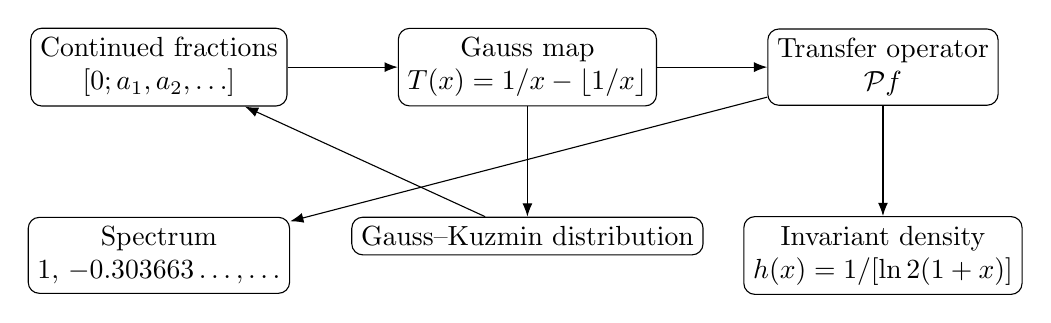
\begin{tikzpicture}[node distance=1.4cm, every node/.style={align=center}, >=Latex]
\node (cf) [draw, rounded corners] {Continued fractions\\$[0;a_1,a_2,\ldots]$};
\node (gm) [draw, rounded corners, right=of cf] {Gauss map\\$T(x)=1/x-\lfloor1/x\rfloor$};
\node (op) [draw, rounded corners, right=of gm] {Transfer operator\\$\PP f$};
\node (inv) [draw, rounded corners, below=of op] {Invariant density\\$h(x)=1/[\ln2(1+x)]$};
\node (dist) [draw, rounded corners, below=of gm] {Gauss--Kuzmin distribution};
\node (spec) [draw, rounded corners, below=of cf] {Spectrum\\$1,\,-0.303663\ldots,\ldots$};
\draw[->] (cf) -- (gm);
\draw[->] (gm) -- (op);
\draw[->] (op) -- (inv);
\draw[->] (gm) -- (dist);
\draw[->] (op) -- (spec);
\draw[->] (dist) -- (cf);
\end{tikzpicture}
\end{center}

\section*{Further directions}
Natural next topics include a proof of ergodicity of the Gauss map, the exact Gauss--Kuzmin error estimates, the function spaces on which the transfer operator has a discrete spectrum, explicit construction of the dominant nontrivial eigenfunction, Mayer's transfer operator, and the connection between dynamical zeta functions and the Riemann zeta function.

\end{document}

\clearpage

% ========================================================
\part{Special Functions \& Classical Analysis}
% ========================================================
\documentclass[a4paper]{article}

% Shared Preamble for MathLatexDocs

% --- Core Packages ---
\usepackage[english]{babel}
\usepackage[utf8]{inputenc}
\usepackage{amsmath}
\usepackage{amsthm}
\usepackage{amssymb}
\usepackage{mathtools}
\usepackage{graphicx}
\usepackage{microtype} % Better justification and fewer overfull hboxes
\usepackage{bm}
\usepackage{enumitem}
\usepackage{booktabs}
\usepackage{mathrsfs}

% --- Layout & Design ---
\usepackage{docmute}
\usepackage{subfiles} % Support for master/subfile structure
\usepackage[colorinlistoftodos]{todonotes}
\usepackage[colorlinks=true, linkcolor=blue, citecolor=magenta]{hyperref}
\usepackage{cleveref} % Better cross-referencing
\usepackage{tcolorbox} % For styled boxes
\usepackage{tikz} % For drawing diagrams
\usetikzlibrary{arrows.meta,positioning}

% --- Theorem Environments (Classic Style) ---
\makeatletter
\@ifundefined{classicthm}{%
  \newtheorem{classicthm}{Theorem}[section]
  \newtheorem{classicdef}[classicthm]{Definition}
  \newtheorem{classiclem}[classicthm]{Lemma}
  \newtheorem{theorem}{Theorem}[section]
  \newtheorem{corollary}{Corollary}[theorem]
  \newtheorem{lemma}[theorem]{Lemma}
  \newtheorem{definition}{Definition}[section]
  \newtheorem{proposition}[theorem]{Proposition}
  \newtheorem{remark}[theorem]{Remark}
  \newtheorem{example}[theorem]{Example}
}{}

% Wrappers to maintain compatibility with the {Title}{Label} syntax used in files
\@ifundefined{mytheorem}{%
  \newenvironment{mytheorem}[2]{%
    \begin{classicthm}[#1]\label{thm:#2}
  }{%
    \end{classicthm}
  }
  
  \newenvironment{mydefinition}[2]{%
    \begin{classicdef}[#1]\label{def:#2}
  }{%
    \end{classicdef}
  }
  
  \newenvironment{mylemma}[2]{%
    \begin{classiclem}[#1]\label{lem:#2}
  }{%
    \end{classiclem}
  }
}{}
\makeatother

% --- Custom Commands ---
\providecommand{\Z}{\mathbb{Z}}
\providecommand{\R}{\mathbb{R}}
\providecommand{\C}{\mathbb{C}}
\providecommand{\N}{\mathbb{N}}
\providecommand{\G}{\mathcal{G}}
\providecommand{\Lop}{\mathcal{L}}
\providecommand{\PP}{\mathcal{P}}
\providecommand{\dd}{\,\mathrm{d}}
\providecommand{\bitand}{\mathbin{\&}}
\providecommand{\CFDots}{\genfrac{}{}{0pt}{0}{}{\ddots}}


\title{Bernoulli Numbers}
\author{Emil Kerimov}
\date{}
\begin{document}
\maketitle

\section{Bernoulli Numbers}\label{bn:sec:bernoulli-numbers}
Examining the Taylor expansion of $\frac{x}{e^x -1}$, this will be required for the evaluation of the even integer values of $\zeta.$

\begin{definition}
    \label{bn:bernoulli-def}
    The Bernoulli numbers $B_n$ are defined as the coefficients of the Taylor expansion of the following function
    \[\boxed{
            \frac{x}{e^x -1} = \sum_{n=0}^{\infty} \frac{B_n}{n!} x^n
        }
    \]
\end{definition}

\begin{theorem}
    \begin{equation}
        \label{bn:eq:bernoulli-generating}
        \sum_{k}^{n} \binom{n+1}{k} B_k = 0  \quad \forall n > 0, \text{ with } B_0 = 1
    \end{equation}

    Proof
    \begin{gather*}
        \intertext{Starting from definition~\ref{bn:bernoulli-def}}
        \frac{x}{e^x -1} = \sum_{n=0}^{\infty} \frac{B_n}{n!} x^n
        \\
        \intertext{Using the Taylor expansion of $e^x$}
        \frac{x}{\sum_{k=1}^{\infty} \frac{x^k}{k!}} = \sum_{n=0}^{\infty} \frac{B_n}{n!} x^n
        \\
        \intertext{Rearranging}
        x = \sum_{k=1}^{\infty} \frac{x^k}{k!} \sum_{n=0}^{\infty} \frac{B_n}{n!} x^n
        \\
        1 = \sum_{k=1}^{\infty} \frac{x^{k-1}}{k!} \sum_{n=0}^{\infty} \frac{B_n}{n!} x
        \\
        \intertext{Adjusting the indices}
        1 = \sum_{k=0}^{\infty} \frac{x^{k}}{(k+1)!} \sum_{n=0}^{\infty} \frac{B_n}{n!} x^n
        \\
        \intertext{Using Cauchy's product formula for infinite sums \footnotemark}
        1 = \sum_{n=0}^{\infty}
        \underbrace{\sum_{k=0}^{n}
            \underbrace{\Big(\frac{B_k}{k!} x^k \Big)}_{a_k}
            \underbrace{\Big(\frac{x^{n-k}}{(n-k+1)!} \Big)}_{b_{n-k}}}_{c_n}
        \\
        \intertext{Simplifying}
        1 = \sum_{n=0}^{\infty}
        \frac{1}{(n+1)!}
        \sum_{k=0}^{n}
        \binom{n+1}{k}
        B_k x^k x^{n-k}
        \\
        1 = \sum_{n=0}^{\infty}
        \frac{x^n}{(n+1)!}
        \sum_{k=0}^{n}  \binom{n+1}{k} B_k
        \intertext{Comparing coefficients of powers of $x$ of both sides we get}
        n=0, \quad  1 =  B_0
        \\
        n \not =0, \quad 0= \sum_{k=0}^{n}  \binom{n+1}{k} B_k
    \end{gather*}
\end{theorem}
\footnotetext{$\left( \sum_{n=0}^{\infty} a_n \right) \left( \sum_{n=0}^{\infty} b_n \right) = \sum_{n=0}^{\infty} c_n $ where $c_n = \sum_{k=0}^{n} a_k b_{n-k}$. See Theorem~\ref{bn:thm:mertens-cauchy-product} for the proof.}

\subsection{First few Bernoulli numbers}\label{bn:subsec:first-few-bernoulli-numbers}
Using equation~\ref{eq:bernoulli-generating} with $n=1$ implies $ \binom{2}{0} B_0 + \binom{2}{1} B_1 = 0 = 1 + 2 B_1 $ which implies
\begin{equation}
    B_1 = -\frac{1}{2}\label{bn:eq:equation}
\end{equation}

Using equation~\ref{eq:bernoulli-generating} with $n=2$ implies $ \binom{3}{0} B_0 + \binom{3}{1} B_1 + \binom{3}{2} B_2 = 0 = 1 - \frac{3}{2} + 3 B_2 $ which implies
\begin{equation}
    B_2 = \frac{1}{6}\label{bn:eq:equation2}
\end{equation}

Similarly when we apply this equation for increasing values of n
\begin{equation}
    B_3 = 0, B_4 = -\frac{1}{30}, B_5 = 0, B_6 = \frac{1}{42}, \dots \label{bn:eq:equation3}
\end{equation}


\begin{theorem}
    In fact we can show that all odd Bernoulli numbers after n=1 are 0
    \begin{equation}
        \label{bn:eq:odd-bernoulli} B_n = 0  \quad \forall \text{ odd }n > 1
    \end{equation}

    Proof
    \begin{gather*}
        \intertext{Starting from definition~\ref{bn:bernoulli-def}}
        \frac{x}{e^x -1} = \sum_{n=0}^{\infty} \frac{B_n}{n!} x^n
        \\
        \intertext{Removing the first two terms of the sum}
        \frac{x}{e^x -1} = B_0 + B_1 x + \sum_{n=2}^{\infty} \frac{B_n}{n!} x^n\\
        \intertext{Rearranging}
        \frac{x}{e^x -1}  - 1 + \frac{x}{2}= \sum_{n=2}^{\infty} \frac{B_n}{n!} x^n
        \\
        \frac{x + xe^x}{2e^x -2}  - 1 = \sum_{n=2}^{\infty} \frac{B_n}{n!} x^n
        \\
        \intertext{If we can show that the RHS is an even function then we have established the proof}
        y(x) = \frac{x + xe^x}{2e^x -2}  - 1
        \\
        y(-x) = \frac{-x + -xe^{-x}}{2e^{-x} -2}  - 1
        \\
        \intertext{Simplifying}
        y(-x) = \frac{-x -xe^{-x}}{2e^{-x} -2} \cdot \frac{e^x}{e^x}  - 1
        \\
        y(-x) = \frac{-xe^x -x}{2 -2e^x}  - 1
        \\
        y(-x) = \frac{x+xe^x}{2e^x - 2}  - 1
        \\
        y(-x) = y(x)
        \\
        B_n = 0  \quad \forall \text{ odd }n > 1
    \end{gather*}
\end{theorem}

\pagebreak


\section{Bernoulli Polynomials}\label{bn:sec:bernoulli-polynomials}
\begin{definition}
    \label{bn:bernoulli poly def}
    The Bernoulli polynomials $B_n(x)$ are defined as
    \[\boxed{
            B_{n}(x) = \sum_{k=0}^{n} \binom{n}{k} B_k x^{n-k}
        }\]
\end{definition}

\subsection{Examples}\label{bn:subsec:examples}
\begin{align*}
    B_{0}(x) & = B_0 = 1
    \\
    B_{1}(x) & = B_0 x + B_1 = x - \frac{1}{2}
    \\
    B_{2}(x) & = B_0 x^2 + \binom{2}{1} B_1 x + B_2 = x^2 - x +  \frac{1}{6}
    \\
    B_{3}(x) & = B_0 x^3 + \binom{3}{1} B_1 x^2 + \binom{3}{2} B_2 x + B_3 = x^3 - \frac{3}{2} x^2 +  \frac{1}{2} x
\end{align*}

Note that $B_n(x)$ is a polynomial of degree $n$.

\subsection{Useful Properties}\label{bn:subsec:useful-properties}
\begin{theorem}
    $B_n(0)$
    \begin{equation}
        \boxed{B_n(0) = B_n}\label{bn:eq:equation4}
    \end{equation}
    Proof
    \begin{gather*}
        B_n(x) = \sum_{k=0}^{n} \binom{n}{k} B_k x^{n-k}
        \\
        B_n(x) = \sum_{k=0}^{n-1} \binom{n}{k} B_k x^{n-k} + B_n
        \\
        B_n(0) = \sum_{k=0}^{n-1} \binom{n}{k} B_k \cdot 0 + B_n = B_n
    \end{gather*}
\end{theorem}

\begin{theorem}
    Boundary value $B_n(1)$:
    \begin{equation}
        \boxed{
        B_n(1) = 
        \begin{cases}
            -B_1 = \frac{1}{2}, & \text{if } n = 1, \\[1ex]
            B_n, & \text{if } n \neq 1.
        \end{cases}
        }\label{bn:eq:equation5}
    \end{equation}
    Proof
    \begin{gather*}
        B_n(x) = \sum_{k=0}^{n} \binom{n}{k} B_k x^{n-k}
        \\
        B_n(1) = \sum_{k=0}^{n} \binom{n}{k} B_k
        \intertext{For $n=1$, direct evaluation gives $B_1(1) = \binom{1}{0} B_0 + \binom{1}{1} B_1 = 1 - \frac{1}{2} = \frac{1}{2} = -B_1$. For $n \geq 2$, using the defining recurrence $\sum_{k=0}^{n-1} \binom{n}{k} B_k = 0$ from equation~\eqref{bn:eq:bernoulli-generating}:}
        \sum_{k}^{n-1} \binom{n}{k} B_k = 0
        \intertext{Adding $B_n$ to both sides}
        \sum_{k}^{n} \binom{n}{k} B_k = B_n
    \end{gather*}
\end{theorem}

\begin{theorem}
    Derivative
    \begin{equation}
        \boxed{B^{'}_n(x) = n B_{n-1}(x)}\label{bn:eq:equation6}
    \end{equation}
    Proof
    \begin{gather*}
        B_n(x) = \sum_{k=0}^{n} \binom{n}{k} B_k x^{n-k}
        \intertext{Taking derivatives of both sides}
        B^{'}_n(x) = \sum_{k=0}^{n-1} \binom{n}{k} B_k (n-k) x^{n-k-1}
        \\
        B^{'}_n(x) = \sum_{k=0}^{n-1} \frac{n! (n-k)}{k! (n-k)!} B_k x^{n-1-k}
        \\
        B^{'}_n(x) = \sum_{k=0}^{n-1} \frac{(n-1)! \cdot n}{k! (n-k-1)!} B_k x^{n-1-k}
        \\
        B^{'}_n(x) = n \sum_{k=0}^{n-1} \binom{n-1}{k} B_k x^{n-1-k}
        \\
        B^{'}_n(x) = n B_{n-1}(x)
    \end{gather*}
\end{theorem}

\begin{theorem}
    Integral
    \begin{equation}
        \boxed{\int_{x=0}^{1} B_n(x) dx = 0}\label{bn:eq:equation7}
    \end{equation}
    Proof
    \begin{gather*}
        \intertext{Starting from the derivative equation, using $m=n-1$}
        B^{'}_{m+1}(x) = (m+1) \cdot B_{m}(x)
        \intertext{Integrating both sides}
        \int_{x=0}^{1} B^{'}_{m+1}(x) = B_{m+1}(1) - B_{m+1}(0) = (m+1) \cdot  \int_{x=0}^{1} B_{m}(x)
        \intertext{Using the Bernoulli polynomial properties}
        B_{m+1}(1) - B_{m+1}(0) = B_{m+1} - B_{m+1} = 0
        \intertext{Therefore for $m \neq -1$}
        \int_{x=0}^{1} B_{m}(x) = 0
    \end{gather*}
\end{theorem}

\pagebreak


\section{Euler-Maclaurin formula}\label{bn:sec:euler-maclaurin-formula}

Let $ \{ x \} = x - \lfloor{x}\rfloor $ then

\begin{theorem}
    \begin{subequations}
        \label{bn:Euler-Maclaurin formula}
        \begin{align}
            \sum_{k=1}^{n-1} f(k) & = \int_{x=1}^{n} f(x) dx -
            \sum_{k=1}^{m} \frac{B_k}{k!} \cdot \big( f^{(k-1)}(n) - f^{(k-1)}(1) \big) +
            R_{mn}                                                                                           \\
            R_{mn}                & = \frac{(-1)^{m+1}}{m!} \cdot \int_{x=1}^{n} B_{m}(\{x\}) f^{(m)} (x) dx
        \end{align}
    \end{subequations}

    Proof
    \begin{gather*}
        \intertext{See the Darboux Formula paper for proof}
    \end{gather*}
\end{theorem}

\subsection{Stirling's Approximation}\label{bn:subsec:stirling's-approximation}
\begin{theorem}
    %\begin{equation} 
    %n! = \Big( \frac{n}{e} \Big)^{n} \sqrt{2 \pi n} \cdot e^{\sum_{k=2}^{m} \frac{B_k}{k \cdot (k-1)} \cdot \frac{1}{n^{k-1}} + O(\frac{1}{n^{m}})} 
    %\end{equation}

    \begin{equation}
        n! = \Big( \frac{n}{e} \Big)^{n} \sqrt{2 \pi n} \cdot exp\Bigg(\sum_{k=1}^{\lfloor m/2 \rfloor} \frac{B_{2k}}{2k \cdot (2k-1)}  \frac{1}{n^{2k-1}} + O(\frac{1}{n^{m}})\Bigg)\label{bn:eq:equation8}
    \end{equation}


    Proof
    \begin{gather*}
        \intertext{See the Gamma function paper for proof}
    \end{gather*}
\end{theorem}

\pagebreak


\section{Evaluation of Even Zeta Values \texorpdfstring{$\zeta(2n)$}{zeta(2n)}}\label{bn:sec:connection-to-zeta-2n}

See the Zeta function document.

\begin{theorem}
    We can express all even integer values of $\zeta$ using Bernoulli numbers
    \begin{equation}
        \label{bn:eq:even-zeta}
        \zeta(2n) = (-1)^{n+1} \frac{(2\pi)^{2n} B_{2n}}{2 \cdot (2n)!}
    \end{equation}

    Proof:
    See the Zeta function document.
\end{theorem}

\subsection{The first few even integer values of Zeta}\label{bn:subsec:the-first-few-even-integer-values-of-zeta}

\begin{gather*}
    \zeta(2) = \frac{\pi^2}{6},
    \zeta(4) = \frac{\pi^4}{90},
    \zeta(6) = \frac{\pi^6}{945},
    \zeta(8) = \frac{\pi^8}{9450},
    \zeta(10) = \frac{\pi^{10}}{93555},
    \\
    \zeta(12) = \frac{691}{638512875} \pi^{12},
    \zeta(14) = \frac{2}{18243225} \pi^{14},
    \zeta(16) = \frac{3617}{325641566250} \pi^{16},
    \\
    \zeta(18) = \frac{43867}{38979295480125} \pi^{18},
    \zeta(20) = \frac{174611}{1531329465290625} \pi^{20},
    \zeta(22) = \frac{155366}{13447856940643125} \pi^{22},
    \\
    \zeta(24) = \frac{236364091}{201919571963756521875} \pi^{24},
    \dots
\end{gather*}

\pagebreak

\section{Cauchy Product of Series (Mertens' Theorem)}\label{bn:sec:cauchy-product}

When multiplying two infinite series $\sum_{n=0}^{\infty} a_n$ and $\sum_{n=0}^{\infty} b_n$, the resulting series arranged by total degree is known as the \emph{Cauchy product}:
\begin{equation}
    c_n = \sum_{k=0}^{n} a_k b_{n-k}
\end{equation}

\begin{theorem}[Mertens' Theorem on Cauchy Products]\label{bn:thm:mertens-cauchy-product}
    Let $\sum_{n=0}^{\infty} a_n = A$ be an absolutely convergent series, and let $\sum_{n=0}^{\infty} b_n = B$ be a convergent series. Then their Cauchy product series converges to their product:
    \begin{equation}
        \sum_{n=0}^{\infty} c_n = \sum_{n=0}^{\infty} \left( \sum_{k=0}^{n} a_k b_{n-k} \right) = A B = \left( \sum_{n=0}^{\infty} a_n \right) \left( \sum_{n=0}^{\infty} b_n \right)
    \end{equation}
\end{theorem}

\begin{proof}
    Let $A_N = \sum_{n=0}^{N} a_n$, $B_N = \sum_{n=0}^{N} b_n$, and $C_N = \sum_{n=0}^{N} c_n$. Let $\beta_N = B_N - B$, so that $\lim_{N \to \infty} \beta_N = 0$.
    
    Expanding the partial sum $C_N$:
    \begin{align*}
        C_N &= \sum_{n=0}^{N} \sum_{k=0}^{n} a_k b_{n-k} \\
            &= \sum_{k=0}^{N} a_k \sum_{n=k}^{N} b_{n-k} \\
            &= \sum_{k=0}^{N} a_k B_{N-k} \\
            &= \sum_{k=0}^{N} a_k (B + \beta_{N-k}) \\
            &= B A_N + \sum_{k=0}^{N} a_k \beta_{N-k}
    \end{align*}
    Let $\gamma_N = \sum_{k=0}^{N} a_k \beta_{N-k}$. We want to show that $\lim_{N \to \infty} \gamma_N = 0$.
    
    Since $\sum_{n=0}^{\infty} a_n$ is absolutely convergent, let $M = \sum_{n=0}^{\infty} |a_n| < \infty$. If $M = 0$, all $a_n = 0$ and the result is trivial. Otherwise, given any $\varepsilon > 0$:
    \begin{enumerate}
        \item Since $\beta_N \to 0$, there exists $N_0 \in \mathbb{N}$ such that $|\beta_m| < \frac{\varepsilon}{2M}$ for all $m > N_0$.
        \item Let $K = \sup_{m \ge 0} |\beta_m| < \infty$. Since the tail of the absolutely convergent series $\sum |a_k|$ vanishes, there exists $N_1 > N_0$ such that for all $N > N_1$:
        \[
            \sum_{k=N-N_0}^{N} |a_k| < \frac{\varepsilon}{2K + 1}
        \]
    \end{enumerate}
    Then for any $N > N_1$:
    \begin{align*}
        |\gamma_N| &\le \sum_{k=0}^{N-N_0-1} |a_k| |\beta_{N-k}| + \sum_{k=N-N_0}^{N} |a_k| |\beta_{N-k}| \\
                   &< \frac{\varepsilon}{2M} \sum_{k=0}^{N-N_0-1} |a_k| + K \sum_{k=N-N_0}^{N} |a_k| \\
                   &< \frac{\varepsilon}{2M} (M) + K \left(\frac{\varepsilon}{2K+1}\right) < \frac{\varepsilon}{2} + \frac{\varepsilon}{2} = \varepsilon
    \end{align*}
    Therefore $\lim_{N \to \infty} \gamma_N = 0$, which yields:
    \[
        \lim_{N \to \infty} C_N = \lim_{N \to \infty} (B A_N + \gamma_N) = B A + 0 = A B
    \]
\end{proof}

\end{document}

\clearpage

\documentclass[a4paper]{article}

% Shared Preamble for MathLatexDocs

% --- Core Packages ---
\usepackage[english]{babel}
\usepackage[utf8]{inputenc}
\usepackage{amsmath}
\usepackage{amsthm}
\usepackage{amssymb}
\usepackage{mathtools}
\usepackage{graphicx}
\usepackage{microtype} % Better justification and fewer overfull hboxes
\usepackage{bm}
\usepackage{enumitem}
\usepackage{booktabs}
\usepackage{mathrsfs}

% --- Layout & Design ---
\usepackage{docmute}
\usepackage{subfiles} % Support for master/subfile structure
\usepackage[colorinlistoftodos]{todonotes}
\usepackage[colorlinks=true, linkcolor=blue, citecolor=magenta]{hyperref}
\usepackage{cleveref} % Better cross-referencing
\usepackage{tcolorbox} % For styled boxes
\usepackage{tikz} % For drawing diagrams
\usetikzlibrary{arrows.meta,positioning}

% --- Theorem Environments (Classic Style) ---
\makeatletter
\@ifundefined{classicthm}{%
  \newtheorem{classicthm}{Theorem}[section]
  \newtheorem{classicdef}[classicthm]{Definition}
  \newtheorem{classiclem}[classicthm]{Lemma}
  \newtheorem{theorem}{Theorem}[section]
  \newtheorem{corollary}{Corollary}[theorem]
  \newtheorem{lemma}[theorem]{Lemma}
  \newtheorem{definition}{Definition}[section]
  \newtheorem{proposition}[theorem]{Proposition}
  \newtheorem{remark}[theorem]{Remark}
  \newtheorem{example}[theorem]{Example}
}{}

% Wrappers to maintain compatibility with the {Title}{Label} syntax used in files
\@ifundefined{mytheorem}{%
  \newenvironment{mytheorem}[2]{%
    \begin{classicthm}[#1]\label{thm:#2}
  }{%
    \end{classicthm}
  }
  
  \newenvironment{mydefinition}[2]{%
    \begin{classicdef}[#1]\label{def:#2}
  }{%
    \end{classicdef}
  }
  
  \newenvironment{mylemma}[2]{%
    \begin{classiclem}[#1]\label{lem:#2}
  }{%
    \end{classiclem}
  }
}{}
\makeatother

% --- Custom Commands ---
\providecommand{\Z}{\mathbb{Z}}
\providecommand{\R}{\mathbb{R}}
\providecommand{\C}{\mathbb{C}}
\providecommand{\N}{\mathbb{N}}
\providecommand{\G}{\mathcal{G}}
\providecommand{\Lop}{\mathcal{L}}
\providecommand{\PP}{\mathcal{P}}
\providecommand{\dd}{\,\mathrm{d}}
\providecommand{\bitand}{\mathbin{\&}}
\providecommand{\CFDots}{\genfrac{}{}{0pt}{0}{}{\ddots}}


\title{Gamma Function}
\author{Emil Kerimov}
\date{\today}
\begin{document}
    \maketitle




    \section{Definition of the Gamma Function}\label{gf:sec:definition}

    \begin{definition}
        \label{gf:gamma-def-1}
        The Gamma Function is defined as:
        \[
        \Gamma(z) = \int_{0}^{\infty} e^{-t} t^{z-1} dt
        \]
    \end{definition}

    The first few evaluations of the Gamma function are:
    \begin{equation}
        \begin{aligned}
            \Gamma(1) &= \int_{0}^{\infty} e^{-t} \ dt  = - e^{-t}\Big|_{0}^{\infty} = 0 - (-1) = 1 \\
            \Gamma(2) &= \int_{0}^{\infty} e^{-t}  t \ dt = - e^{-t}t\Big|_{0}^{\infty} + \int_{0}^{\infty} e^{-t} \ dt = 1 \\
            \Gamma(3) &= \int_{0}^{\infty} e^{-t}  t^2 \ dt = - e^{-t}t^2\Big|_{0}^{\infty} + 2\int_{0}^{\infty} e^{-t}t \ dt = 2 \\
            \Gamma(4) &= \int_{0}^{\infty} e^{-t}  t^3 \ dt = - e^{-t}t^3\Big|_{0}^{\infty} + 3\int_{0}^{\infty} e^{-t}t \ dt = 6 \\
        \end{aligned}\label{gf:eq:equation}
    \end{equation}


    \section{Relation to the Factorial Function}\label{gf:sec:relation-to-the-factorial-function}
    Expanding on the pattern we found by evaluating the first few integer values of the Gamma function through integration by parts we obtain:

    \begin{theorem}
        \label{gf:Def}
        $ \Gamma(z+1) = z \Gamma(z) $

        Proof by induction
        \begin{gather*}
            \shortintertext{Assume true for k}
            \Gamma(k+1) = k \Gamma(k)
            \shortintertext{Proving for k+1}
            \begin{split}
                \Gamma(k+1) &= \int_{0}^{\infty} e^{-t}  t^k \ dt  \\
                &= - e^{-t}t^k\Big|_{0}^{\infty} + k\int_{0}^{\infty} e^{-t}t^{k-1} \ dt\\
                &= 0 - 0 + k\Gamma(k-1) \\
                &= k\Gamma(k-1) \\
            \end{split}
        \end{gather*}
    \end{theorem}

    \subsection{Integer Values}\label{gf:subsec:integer-values}
    Therefore since $\Gamma(1) = 1$, then for positive integer values

    \begin{equation}
        \Gamma(n) = (n-1)!\label{gf:eq:equation2}
    \end{equation}


    \section{Equivalent Integral Forms}\label{gf:sec:equivalent-integral-forms}

    \begin{equation}
        \Gamma(z) = \int_{0}^{\infty} e^{-t} t^{z-1} dt\label{gf:eq:equation3}
    \end{equation}

    \begin{theorem}
        Starting from Equation~\ref{gf:gamma-def-1}, we can use the substitution $t = -ln(u)$ to obtain
        \begin{equation}
            \Gamma(z) = \int_{0}^{1} (-ln u)^{z-1} dt\label{gf:eq:equation4}
        \end{equation}

        Proof
        \begin{gather*}
            t = -ln(u) \\
            dt = - \frac{du}{u} \\
            \Gamma(z) = \int_{1}^{0} e^{ln(u)} (-ln(u))^{z-1} \frac{-du}{u} \\
            \Gamma(z) = - \int_{1}^{0} u (-ln(u))^{z-1} \frac{du}{u} \\
            \Gamma(z) = - \int_{1}^{0} (-ln(u))^{z-1} du \\
            \Gamma(z) = \int_{0}^{1} (-ln(u))^{z-1} du \\
        \end{gather*}
    \end{theorem}


    \section{Finite Gamma Expression}\label{gf:sec:finite-gamma-expression}
    Define the finite gamma function (find out its real name)
    \begin{equation}
        \label{gf:eq:finite-gamma-def}
        \Gamma_{p}(x) = \frac{p! p^x}{x (x+ 1)(x + 2)...(x + p)} = \frac{p^x}{x (\frac{x}{1} + 1)(\frac{x}{2} + 1)...(\frac{x}{p} + 1)}
        \ \ x>0
    \end{equation}

    Note that this function has the following properties:
    \begin{equation}
        \Gamma_{p}(1) = \frac{p! p}{1 (1 + 1)(1+2)...(1+p)} = \frac{p! p}{p! (1+p)} = \frac{p}{1+p}\label{gf:eq:equation5}
    \end{equation}

    \begin{equation}
        \label{gf:eq:relation-to-next}
        \begin{split}
            \Gamma_{p}(x+1) &= \frac{p! p p^x}{(x + 1)(x+2)...(x+p)(x+p+1)} \\
            &= \frac{x p! p p^x}{x(x + 1)(x+2)...(x+p)(x+p+1)} \\
            &= \frac{x p}{x+p+1} \Gamma_{p}(x) \\
        \end{split}
    \end{equation}

    \subsection{Taking the limit to obtain Gamma}\label{gf:subsec:taking-the-limit-to-obtain-gamma}

    Using Equation~\ref{gf:eq:relation-to-next} and assuming $\Gamma_{\infty}(x)$ converges we get:

    \begin{equation}
        \lim_{p \to \infty} \Gamma_{p}(x+1) =
        \lim_{p \to \infty} \frac{x p}{x+p+1} \Gamma_{p}(x) = x \lim_{p \to \infty} \Gamma_{p}(x)\label{gf:eq:equation6}
    \end{equation}

    Therefore using the above properties we see that if $\Gamma_{\infty}(x)$ converges then it must be equal to $\Gamma(x)$.


    \section{Euler Mascheroni constant}\label{gf:sec:euler-const}
    The Euler Mascheroni constant is defined as:
    \begin{equation}
        \label{gf:eq:euler_mascheroni_def}
        \gamma = \lim_{p \to \infty} \sum_{i=1}^{p} 1/i - ln(p) \approx 0.5772
    \end{equation}

    This constant can be interpreted as the difference between the sum of $1/x$ and the integral of $1/x$ from $1$ to $\infty$.
    It is unknown whether this number is transcendental or even irrational!
    One can show numerically that if it is rational then the denominator must be greater than $10^{242080}$.


    \section{Weierstrass Formula}\label{gf:sec:weierstrass}
    \begin{theorem}
        \label{gf:partial form}
        Let $\gamma$ be the Euler Mascheroni constant as defined in section~\ref{gf:sec:euler-const}, and $\Gamma$ be the Gamma function, then
        \begin{equation}
            \label{gf:eq:gamma-product}
            \frac{1}{\Gamma(x)}  = x \cdot e^{x \gamma} \cdot \prod_{k=1}^{\infty} (1 + x/k) \cdot e^{-x/k}
        \end{equation}

        Proof
        \\
        Re-writing $p^x$
%Starting from equation \ref{gf:gamma-def-1}, and re-writing $p^x$
        \begin{gather*}
            p^x = e^{x lnp} = e^{x [lnp - 1 - 1/2 - 1/3 - \dots - 1/p]} e^{x + x/2 + x/3 + \dots + x/p} \\
            \text{Plugging $p^x$ into equation~\ref{gf:eq:finite-gamma-def}} \\
            \Gamma_{p}(x) = \frac{e^{x [lnp - 1 - 1/2 - 1/3 - \dots - 1/p]} e^{x + x/2 + x/3 + \dots + x/p}}{x (\frac{x}{1} + 1)(\frac{x}{2} + 1)...(\frac{x}{p} + 1)}   \\
            \Gamma_{p}(x) = e^{x [lnp - 1 - 1/2 - 1/3 - \dots - 1/p]} \cdot \frac{1}{x} \cdot \frac{e^{x}}{x+1} \cdot \frac{e^{x/2}}{x/2+1} \cdot \frac{e^{x/3}}{x/3+1}
            \cdot \cdot \cdot \cdot \frac{e^{x/p}}{x/p+1}
            \\
            \Gamma_{p}(x) = e^{x [lnp - 1 - 1/2 - 1/3 - \dots - 1/p]} \cdot \frac{1}{x} \cdot \prod_{k=1}^{p} \frac{e^{x/k}}{1 + x/k} \\
            \text{Taking the limit as $p \to \infty$ }\\
            \Gamma(x) = \lim_{p \to \infty} \Gamma_{p}(x) =
            \lim_{p \to \infty} e^{x [lnp - 1 - 1/2 - 1/3 - \dots - 1/p]} \cdot \frac{1}{x} \cdot \prod_{k=1}^{p} \frac{e^{x/k}}{1 + x/k} \\
            \Gamma(x) = e^{-x \gamma} \cdot  \frac{1}{x} \cdot \prod_{k=1}^{\infty} \frac{e^{x/k}}{1 + x/k}  \\
            \text{Equivalently}\\
            \frac{1}{\Gamma(x)}  = x \cdot e^{x \gamma} \cdot \prod_{k=1}^{\infty} (1 + x/k) \cdot e^{-x/k}  \\
        \end{gather*}
    \end{theorem}

    \subsection{Symmetry around 1/2 relation}\label{gf:subsec:symmetric-gamma}
    Using~\ref{gf:sec:weierstrass} we derive the following functional form.

    \begin{theorem}
        \begin{equation}
            \label{gf:eq:symmetric-gamma-eq}
            \boxed{
                \frac{1}{\Gamma(x)}\cdot \frac{1}{\Gamma(1-x)} = \frac{sin(\pi x)}{\pi}
            }
        \end{equation}

        Proof
        \\
        Starting from~\ref{gf:sec:weierstrass} and considering $\frac{1}{\Gamma(x)}\cdot \frac{1}{\Gamma(-x)}$ we obtain
        \begin{gather*}
            \frac{1}{\Gamma(x)}\cdot \frac{1}{\Gamma(-x)} = x \cdot e^{x \gamma} \cdot \prod_{k=1}^{\infty} (1 + x/k) \cdot e^{-x/k}   \cdot -x \cdot e^{-x \gamma} \cdot \prod_{k=1}^{\infty} (1 - x/k) \cdot e^{x/k}
            \\
            \frac{1}{\Gamma(x)}\cdot \frac{1}{\Gamma(-x)} = -x^2 \cdot \prod_{k=1}^{\infty} (1 - x^2/k^2) \\
            \text{Using the functional form of $\Gamma$, we get $\Gamma(1-x) = \Gamma(-x+1) = -x \Gamma(-x)$}
            \\
            \frac{1}{\Gamma(x)}\cdot \frac{1}{\Gamma(1-x)} = x \cdot \prod_{k=1}^{\infty} (1 - x^2/k^2) \\
            \text{Using the product form of $\frac{\sin(\pi x)}{\pi x} = \prod_{k=1}^{\infty} \left( 1-\frac{x^2}{k^2} \right)$
                , See Euler's Sine Product Form document}
            \\
            \frac{1}{\Gamma(x)}\cdot \frac{1}{\Gamma(1-x)} = \frac{sin(\pi x)}{\pi}
        \end{gather*}
    \end{theorem}

    \subsection{Special Examples}\label{gf:subsec:special-examples}
    Plugging in various values for $x$ we obtain certain values and relations for $\Gamma(x)$

    $x = \frac{1}{2}$
    \begin{equation}
        \label{gf:eq:gamma-half}
        \Gamma(\frac{1}{2}) = \sqrt{\frac{\pi}{sin(\frac{\pi}{2})}} = \sqrt{\pi}
    \end{equation}

    $x = \frac{1}{3}$
    \begin{equation}
        \Gamma(\frac{1}{3}) \Gamma(\frac{2}{3}) = \frac{\pi}{sin(\frac{\pi}{3})} = \frac{2\pi}{\sqrt{3}} \label{gf:eq:equation7}
    \end{equation}

    $x = \frac{1}{4}$
    \begin{equation}
        \Gamma(\frac{1}{4}) \Gamma(\frac{3}{4}) = \frac{\pi}{sin(\frac{\pi}{4})} = \sqrt{2} \pi \label{gf:eq:equation8}
    \end{equation}

    \begin{theorem}
        $x = -\frac{1}{2}$ with equation~\ref{gf:eq:gamma-half}
        \begin{equation}
            \label{gf:eq:negative-gamma-half}
            \Gamma(-\frac{1}{2}) = -2 \sqrt{\pi}
        \end{equation}

        Proof
        \\
        \begin{gather*}
            \Gamma(-\frac{1}{2}) \cdot \Gamma(1-(-\frac{1}{2})) = \frac{\pi}{sin(-\frac{\pi}{2})}
            \\
            \Gamma(-\frac{1}{2}) = -\frac{\pi}{\Gamma(\frac{3}{2})}
            \\
            \Gamma(-\frac{1}{2}) = -\frac{\pi}{\frac{1}{2} \Gamma(\frac{1}{2})}
            \\
            \Gamma(-\frac{1}{2}) = -\frac{\pi}{\frac{1}{2} \sqrt{\pi}}
            \\
            \Gamma(-\frac{1}{2}) = -2\sqrt{\pi}
        \end{gather*}

    \end{theorem}



    Note that equation~\ref{gf:eq:gamma-half} implies that
    \begin{equation}
        \Gamma(\frac{1}{2}) = \int_{0}^{\infty} \frac{1}{e^t \sqrt{t}} dt = \sqrt{\pi} \label{gf:eq:equation9}
    \end{equation}
    Since $\Gamma(x) = (x-1)!$ for integer values of $x$, this is where the idea of $(-\frac{1}{2})! = \sqrt{\pi}$ comes from.


    \section{Other relations}\label{gf:sec:other-relations}

    \subsection{Gauss's Multiplication Formula}\label{gf:subsec:gauss-multiplication-formula}

    The multiplication formula, discovered by Carl Friedrich Gauss in 1812, generalizes Legendre's duplication formula (Section~\ref{gf:subsec:proof-of-leg-dup}) to an arbitrary positive integer multiplier $n \ge 1$.

    \begin{theorem}
        For any integer $n \ge 1$ and any complex number $x \notin \{0, -1/n, -2/n, \dots\}$:
        \begin{equation}
            \label{gf:eq:legendre-mult}
            \boxed{
                \Gamma(x) \cdot \Gamma\left(x+\frac{1}{n}\right) \cdot \Gamma\left(x+\frac{2}{n}\right) \cdots \Gamma\left(x+\frac{n-1}{n}\right) = (2 \pi)^{\frac{n-1}{2}} n^{\frac{1}{2} - nx} \Gamma(nx)
            }
        \end{equation}

        Proof
        \\
        We prove the multiplication formula using Euler's limit product representation of the Gamma function from Section~\ref{gf:sec:finite-gamma-expression}:
        \begin{equation*}
            \Gamma(z) = \lim_{p \to \infty} \frac{p! \, p^z}{z(z+1)(z+2)\cdots(z+p)} = \lim_{p \to \infty} \frac{p! \, p^z}{\prod_{j=0}^p (z+j)}
        \end{equation*}
        For each $k \in \{0, 1, \dots, n-1\}$, evaluating at $z = x + \frac{k}{n}$:
        \begin{align*}
            \Gamma\left(x + \frac{k}{n}\right) & = \lim_{p \to \infty} \frac{p! \, p^{x + k/n}}{\prod_{j=0}^p \left(x + \frac{k}{n} + j\right)} \\
            & = \lim_{p \to \infty} \frac{p! \, p^{x + k/n}}{\prod_{j=0}^p \frac{nx + jn + k}{n}} \\
            & = \lim_{p \to \infty} \frac{n^{p+1} p! \, p^{x + k/n}}{\prod_{j=0}^p (nx + jn + k)}
        \end{align*}
        Multiplying these $n$ limits together for $k = 0, 1, \dots, n-1$:
        \begin{align*}
            \prod_{k=0}^{n-1} \Gamma\left(x + \frac{k}{n}\right) & = \lim_{p \to \infty} \frac{\prod_{k=0}^{n-1} \left( n^{p+1} p! \, p^{x + k/n} \right)}{\prod_{k=0}^{n-1} \prod_{j=0}^p (nx + jn + k)}
        \end{align*}
        Notice that as $k$ ranges from $0$ to $n-1$ and $j$ ranges from $0$ to $p$, the index $jn + k$ covers every integer from $0$ to $n(p+1) - 1$ exactly once.
        Therefore, the denominator is:
        \begin{equation*}
            \prod_{k=0}^{n-1} \prod_{j=0}^p (nx + jn + k) = \prod_{m=0}^{n(p+1)-1} (nx + m)
        \end{equation*}
        For the numerator:
        \begin{align*}
            \prod_{k=0}^{n-1} \left( n^{p+1} p! \, p^{x + k/n} \right) & = n^{n(p+1)} (p!)^n p^{nx + \sum_{k=0}^{n-1} \frac{k}{n}} \\
            & = n^{n(p+1)} (p!)^n p^{nx + \frac{n-1}{2}}
        \end{align*}
        Now compare this with Euler's limit formula for $\Gamma(nx)$ with parameter $np$:
        \begin{equation*}
            \Gamma(nx) = \lim_{p \to \infty} \frac{(np)! \, (np)^{nx}}{\prod_{m=0}^{np} (nx + m)}
        \end{equation*}
        Taking the ratio of the two expressions:
        \begin{align*}
            \frac{\prod_{k=0}^{n-1} \Gamma\left(x + \frac{k}{n}\right)}{\Gamma(nx)} & = \lim_{p \to \infty} \frac{n^{n(p+1)} (p!)^n p^{nx + \frac{n-1}{2}}}{(np)! \, (np)^{nx}} \cdot \frac{\prod_{m=0}^{np} (nx + m)}{\prod_{m=0}^{n(p+1)-1} (nx + m)} \\
            & = n^{-nx} \lim_{p \to \infty} \frac{n^{np+n} (p!)^n p^{\frac{n-1}{2}}}{(np)!} \cdot \frac{1}{\prod_{m=np+1}^{n(p+1)-1} (nx + m)}
        \end{align*}
        The remaining product has $(n(p+1)-1) - np = n-1$ factors:
        \begin{equation*}
            \prod_{m=np+1}^{n(p+1)-1} (nx + m) = (nx + np + 1)(nx + np + 2)\cdots(nx + np + n - 1)
        \end{equation*}
        As $p \to \infty$, this product is asymptotic to $(np)^{n-1} = n^{n-1} p^{n-1}$.
        Substituting this asymptotic behavior:
        \begin{align*}
            \frac{\prod_{k=0}^{n-1} \Gamma\left(x + \frac{k}{n}\right)}{\Gamma(nx)} & = n^{-nx} \lim_{p \to \infty} \frac{n^{np+n} (p!)^n p^{\frac{n-1}{2}}}{(np)! \cdot n^{n-1} p^{n-1}} \\
            & = n^{1-nx} \lim_{p \to \infty} \frac{n^{np} (p!)^n p^{\frac{1-n}{2}}}{(np)!}
        \end{align*}
        Using Stirling's asymptotic formula for factorials (Section~\ref{gf:sec:approximations}):
        \begin{align*}
            p! & \sim \sqrt{2\pi p} \left(\frac{p}{e}\right)^p \implies (p!)^n \sim (2\pi)^{n/2} p^{n/2} \left(\frac{p}{e}\right)^{np} \\
            (np)! & \sim \sqrt{2\pi np} \left(\frac{np}{e}\right)^{np} = \sqrt{2\pi n} \, n^{np} p^{1/2} \left(\frac{p}{e}\right)^{np}
        \end{align*}
        Substituting these into the limit:
        \begin{align*}
            \lim_{p \to \infty} \frac{n^{np} (p!)^n p^{\frac{1-n}{2}}}{(np)!} & = \lim_{p \to \infty} \frac{n^{np} \cdot (2\pi)^{n/2} p^{n/2} (p/e)^{np} \cdot p^{\frac{1-n}{2}}}{\sqrt{2\pi n} \, n^{np} p^{1/2} (p/e)^{np}} \\
            & = \frac{(2\pi)^{n/2}}{\sqrt{2\pi n}} \lim_{p \to \infty} \frac{p^{n/2 + (1-n)/2}}{p^{1/2}} \\
            & = (2\pi)^{\frac{n-1}{2}} n^{-1/2}
        \end{align*}
        Multiplying by $n^{1-nx} \Gamma(nx)$:
        \begin{equation*}
            \prod_{k=0}^{n-1} \Gamma\left(x + \frac{k}{n}\right) = n^{1-nx} \cdot (2\pi)^{\frac{n-1}{2}} n^{-1/2} \Gamma(nx) = (2\pi)^{\frac{n-1}{2}} n^{\frac{1}{2} - nx} \Gamma(nx)
        \end{equation*}
        which completes the proof.
    \end{theorem}

    \begin{corollary}
        Multiplying both sides of Equation~\eqref{gf:eq:legendre-mult} by $x$ and taking the limit as $x \to 0$, we have $\lim_{x \to 0} x \Gamma(x) = \Gamma(1) = 1$, and $\lim_{x \to 0} x \Gamma(nx) = \frac{1}{n} \lim_{x \to 0} (nx)\Gamma(nx) = \frac{1}{n}$.
        Therefore:
        \begin{equation}
            \label{gf:eq:equation10}
            \boxed{
                \Gamma\left(\frac{1}{n}\right) \cdot \Gamma\left(\frac{2}{n}\right) \cdots \Gamma\left(\frac{n-1}{n}\right) = \frac{(2 \pi)^{\frac{n-1}{2}}}{\sqrt{n}}
            }
        \end{equation}
    \end{corollary}

    \begin{example}
        For $n = 2$, Gauss's multiplication formula reduces directly to Legendre's duplication formula (Theorem~\ref{gf:subsec:proof-of-leg-dup}):
        \begin{equation*}
            \Gamma(x) \Gamma\left(x + \frac{1}{2}\right) = (2\pi)^{1/2} 2^{\frac{1}{2} - 2x} \Gamma(2x) = \frac{\sqrt{\pi}}{2^{2x-1}} \Gamma(2x)
        \end{equation*}
        For $n = 3$, Equation~\eqref{gf:eq:equation10} gives:
        \begin{equation*}
            \Gamma\left(\frac{1}{3}\right) \Gamma\left(\frac{2}{3}\right) = \frac{(2\pi)^{2/2}}{\sqrt{3}} = \frac{2\pi}{\sqrt{3}}
        \end{equation*}
        which perfectly agrees with Euler's reflection formula~\eqref{gf:eq:symmetric-gamma-eq}:
        \begin{equation*}
            \Gamma\left(\frac{1}{3}\right) \Gamma\left(1 - \frac{1}{3}\right) = \frac{\pi}{\sin(\pi/3)} = \frac{\pi}{\sqrt{3}/2} = \frac{2\pi}{\sqrt{3}}
        \end{equation*}
    \end{example}

    \subsection{Relation to the Riemann Zeta Function}\label{gf:subsec:relation-to-zeta}

    \begin{theorem}
        For $\mathrm{Re}(s) > 1$, the Gamma function is related to the Riemann Zeta function $\zeta(s) = \sum_{n=1}^\infty \frac{1}{n^s}$ by:
        \begin{equation}
            \label{gf:eq:equation11}
            \boxed{
                \Gamma(s) \zeta(s) = \int_{0}^{\infty} \frac{u^{s-1}}{e^{u} - 1} \dd u
            }
        \end{equation}

        Proof
        \\
        Starting from the integral definition of the Gamma function (Equation~\ref{gf:gamma-def-1}):
        \begin{equation*}
            \Gamma(s) = \int_{0}^{\infty} t^{s-1} e^{-t} \dd t \qquad (\mathrm{Re}(s) > 0)
        \end{equation*}
        For any positive integer $n \ge 1$, substitute $t = n u$, so that $\dd t = n \dd u$:
        \begin{equation*}
            \Gamma(s) = \int_{0}^{\infty} (n u)^{s-1} e^{-n u} n \dd u = n^s \int_{0}^{\infty} u^{s-1} e^{-n u} \dd u
        \end{equation*}
        Dividing by $n^s$:
        \begin{equation*}
            \frac{\Gamma(s)}{n^s} = \int_{0}^{\infty} u^{s-1} e^{-n u} \dd u
        \end{equation*}
        Summing both sides over all positive integers $n \ge 1$:
        \begin{equation*}
            \Gamma(s) \sum_{n=1}^{\infty} \frac{1}{n^s} = \sum_{n=1}^{\infty} \int_{0}^{\infty} u^{s-1} e^{-n u} \dd u
        \end{equation*}
        For $\mathrm{Re}(s) > 1$, we can interchange the summation and the integral by the monotone convergence theorem (or dominated convergence):
        \begin{align*}
            \Gamma(s) \zeta(s) & = \int_{0}^{\infty} u^{s-1} \left( \sum_{n=1}^{\infty} e^{-n u} \right) \dd u \\
            & = \int_{0}^{\infty} u^{s-1} \left( \frac{e^{-u}}{1 - e^{-u}} \right) \dd u \\
            & = \int_{0}^{\infty} \frac{u^{s-1}}{e^u - 1} \dd u
        \end{align*}
        which proves the identity.
    \end{theorem}


    \section{Digamma function}\label{gf:sec:digamma-function}

    \subsection{Definition}\label{gf:subsec:definition}
    Define the Digamma function
    \begin{equation}
        \label{gf:eq:digamma-def}
        \Psi(x) = \frac{\partial}{\partial x}  ln(\Gamma(x)) = \frac{\Gamma'(x)}{\Gamma(x)}
    \end{equation}

    \subsection{Series Representation}\label{gf:subsec:series-representation}

    \begin{theorem}
        Let $\gamma$ be the Euler Mascheroni constant as defined in section~\ref{gf:sec:euler-const} then,
        \begin{equation}
            \label{gf:eq:psi-series}
            \boxed{
                \Psi(x) = -\gamma - \frac{1}{x} + \sum_{k=1}^{\infty} \Big( \frac{1}{k} - \frac{1}{x+k}  \Big)
            }
        \end{equation}

        Proof
        \\
        \begin{gather*}
            \Psi(x) = \frac{\partial}{\partial x}  ln(\Gamma(x))
            \\
            \text{Using equation~\ref{gf:eq:gamma-product}}
            \\
            \Psi(x) = -\frac{\partial}{\partial x} ln(x \cdot e^{x \gamma} \cdot \prod_{k=1}^{\infty} (1 + x/k) \cdot e^{-x/k})
            \\
            \Psi(x) = -\frac{\partial}{\partial x} \Big[ ln(x) + x \gamma + \sum_{k=1}^{\infty} ln(1 + x/k) - \frac{x}{k}
            \Big]
            \\
            \Psi(x) = -\frac{1}{x}  -  \gamma - \sum_{k=1}^{\infty} \frac{1}{k} \cdot \frac{1}{1 + x/k} - \frac{1}{k}
            \\
            \Psi(x) = -\frac{1}{x}  -  \gamma + \sum_{k=1}^{\infty} \frac{1}{k} - \frac{1}{x + k}
        \end{gather*}
    \end{theorem}

    \subsection{Derivatives}\label{gf:subsec:derivatives}
    \begin{theorem}
        \begin{equation}
            \label{gf:eq:psi-first-deriv}
            \boxed{
                \Psi'(x) = \sum_{k=1}^{\infty} \frac{1}{(k+x-1)^2}
            }
        \end{equation}

        Proof
        \\
        \begin{gather*}
            \text{Using equation~\ref{gf:eq:psi-series}}
            \\
            \Psi(x) = -\gamma - \frac{1}{x} + \sum_{k=1}^{\infty} \Big( \frac{1}{k} - \frac{1}{x+k}  \Big)
            \\
            \Psi'(x) = \frac{1}{x^2} + \sum_{k=1}^{\infty} \frac{1}{(x+k)^2}
            \\
            \text{Including the first term in the sum}
            \\
            \Psi'(x) = \sum_{k=1}^{\infty} \frac{1}{(x+k - 1)^2}
        \end{gather*}
    \end{theorem}

    \begin{theorem}
        \begin{equation}
            \label{gf:eq:psi-nth-deriv}
            \boxed{
                \Psi^{n}(x) = \sum_{k=1}^{\infty} \frac{(-1)^{n+1} n! }{(k+x-1)^{n+1}}
            }
        \end{equation}

        Proof
        \\
        Take repeated derivatives of equation~\ref{gf:eq:psi-first-deriv}
    \end{theorem}

    \subsection{Special values}\label{gf:subsec:special-values}
    \begin{theorem}
        \begin{equation}
            \Psi^{n}(x+1) = \Psi^{n}(x) + \frac{(-1)^n n!}{x^{n+1}} \label{gf:eq:equation12}
        \end{equation}

        Proof
        \\
        \begin{gather*}
            \Psi^{n}(x + 1) = \sum_{k=1}^{\infty} \frac{(-1)^{n+1} n! }{(k+x)^{n+1}}
            \\
            \Psi^{n}(x + 1) = \frac{(-1)^n n!}{x^{n+1}}  + \sum_{k=2}^{\infty} \frac{(-1)^{n+1} n! }{(k+x)^{n+1}}
            \\
            \Psi^{n}(x + 1) = \frac{(-1)^n n!}{x^{n+1}}  + \sum_{k=1}^{\infty} \frac{(-1)^{n+1} n! }{(k+x - 1)^{n+1}}
            \\
            \Psi^{n}(x + 1) = \frac{(-1)^n n!}{x^{n+1}}  + \Psi^{n}(x)
        \end{gather*}
    \end{theorem}

    \begin{theorem}
        Reflection formula
        \begin{equation}
            \Psi(1-x) = \Psi(x) + \pi cot(\pi x) \label{gf:eq:equation13}
        \end{equation}

        Proof
        \begin{gather*}
            \Psi(1-x) = -\gamma - \frac{1}{1-x} + \sum_{k=1}^{\infty} \Big( \frac{1}{k} - \frac{1}{k+1-x}  \Big)
            \\
            \intertext{Adding and subtracting $\Psi(x)$}
            \Psi(1-x) = -\gamma - \frac{1}{1-x} + \sum_{k=1}^{\infty} \Big( \frac{1}{k} - \frac{1}{k+1-x}  \Big) + \Psi(x) - \Psi(x)
            \\
            \Psi(1-x) = -\gamma - \frac{1}{1-x} + \sum_{k=1}^{\infty} \Big( \frac{1}{k} - \frac{1}{k+1-x}  \Big) + \Psi(x) - \Bigg(-\gamma - \frac{1}{x} + \sum_{k=1}^{\infty} \Big( \frac{1}{k} - \frac{1}{x+k}  \Big) \Bigg)
            \\
            \intertext{Simplifying}
            \Psi(1-x) = \Psi(x) + \frac{1}{x} - \frac{1}{1-x} + \sum_{k=1}^{\infty} \Big( \frac{1}{k} - \frac{1}{k+1-x}  -  \frac{1}{k} + \frac{1}{x+k} \Big)
            \\
            \Psi(1-x) = \Psi(x) + \frac{1}{x} - \frac{1}{1-x} + \sum_{k=1}^{\infty} \Big(\frac{1}{x+k} - \frac{1}{k+1-x} \Big)
            \\
            \Psi(1-x) = \Psi(x) + \sum_{k=0}^{\infty} \Big(\frac{1}{x+k} + \frac{1}{x -k -1} \Big)
            \\
            \Psi(1-x) = \Psi(x) + \sum_{k=-\infty}^{\infty} \Big(\frac{1}{x+k} \Big)
            \\
            \text{Using the series \footnotemark for }\pi cot(\pi x) = \sum_{k=-\infty}^{\infty} \frac{1}{x + k}
            \\
            \Psi(1-x) = \Psi(x) + \pi cot(\pi x)
        \end{gather*}
    \end{theorem}

    \footnotetext{See the Euler's Sine Product formula document.}

    \begin{theorem}[Duplication Formula for the Digamma Function]\label{gf:thm:digamma-duplication}
        For any complex number $x \notin \{0, -1/2, -1, -3/2, \dots\}$:
        \begin{equation}
            \label{gf:eq:equation14}
            \boxed{
                \Psi(2x) = \frac{1}{2} \Psi(x) + \frac{1}{2} \Psi\left(x + \frac{1}{2}\right) + \ln(2)
            }
        \end{equation}

        Proof
        \\
        We prove the duplication formula by taking the logarithmic derivative of Legendre's duplication formula (Theorem~\ref{gf:subsec:proof-of-leg-dup}):
        \begin{equation*}
            \Gamma(2x) = \frac{2^{2x-1}}{\sqrt{\pi}} \Gamma(x) \Gamma\left(x + \frac{1}{2}\right)
        \end{equation*}
        Taking the natural logarithm of both sides:
        \begin{align*}
            \ln \Gamma(2x) & = \ln\left( \frac{2^{2x-1}}{\sqrt{\pi}} \Gamma(x) \Gamma\left(x + \frac{1}{2}\right) \right) \\
            & = (2x - 1) \ln(2) - \frac{1}{2}\ln(\pi) + \ln \Gamma(x) + \ln \Gamma\left(x + \frac{1}{2}\right)
        \end{align*}
        Differentiating both sides with respect to $x$ using the chain rule and the definition of the Digamma function $\Psi(z) = \frac{\dd}{\dd z} \ln \Gamma(z) = \frac{\Gamma'(z)}{\Gamma(z)}$ (Equation~\ref{gf:eq:digamma-def}):
        \begin{equation*}
            \frac{\dd}{\dd x} \ln \Gamma(2x) = 2 \frac{\Gamma'(2x)}{\Gamma(2x)} = 2 \Psi(2x)
        \end{equation*}
        Differentiating the right-hand side term by term:
        \begin{align*}
            \frac{\dd}{\dd x} \left[ (2x - 1) \ln(2) - \frac{1}{2}\ln(\pi) + \ln \Gamma(x) + \ln \Gamma\left(x + \frac{1}{2}\right) \right] & = 2\ln(2) + \frac{\Gamma'(x)}{\Gamma(x)} + \frac{\Gamma'\left(x + \frac{1}{2}\right)}{\Gamma\left(x + \frac{1}{2}\right)} \\
            & = 2\ln(2) + \Psi(x) + \Psi\left(x + \frac{1}{2}\right)
        \end{align*}
        Equating the derivatives gives:
        \begin{equation*}
            2 \Psi(2x) = \Psi(x) + \Psi\left(x + \frac{1}{2}\right) + 2\ln(2)
        \end{equation*}
        Dividing both sides by $2$:
        \begin{equation*}
            \Psi(2x) = \frac{1}{2} \Psi(x) + \frac{1}{2} \Psi\left(x + \frac{1}{2}\right) + \ln(2)
        \end{equation*}
        which completes the proof.
    \end{theorem}

    \begin{remark}
        More generally, taking the logarithmic derivative of Gauss's multiplication formula (Theorem~\ref{gf:eq:legendre-mult}):
        \begin{equation*}
            \prod_{k=0}^{n-1} \Gamma\left(x + \frac{k}{n}\right) = (2\pi)^{\frac{n-1}{2}} n^{\frac{1}{2} - nx} \Gamma(nx)
        \end{equation*}
        yields Gauss's multiplication formula for the Digamma function:
        \begin{equation}
            \label{gf:eq:digamma-multiplication}
            \boxed{
                \Psi(nx) = \frac{1}{n} \sum_{k=0}^{n-1} \Psi\left(x + \frac{k}{n}\right) + \ln(n)
            }
        \end{equation}
        for any integer $n \ge 1$. The duplication formula is the special case $n = 2$.
    \end{remark}

    \begin{example}
        Setting $x = 1/2$ in the duplication formula~\eqref{gf:eq:equation14}:
        \begin{align*}
            \Psi(1) & = \frac{1}{2} \Psi\left(\frac{1}{2}\right) + \frac{1}{2} \Psi(1) + \ln(2) \\
            \frac{1}{2} \Psi(1) & = \frac{1}{2} \Psi\left(\frac{1}{2}\right) + \ln(2) \\
            \Psi\left(\frac{1}{2}\right) & = \Psi(1) - 2\ln(2)
        \end{align*}
        Since $\Psi(1) = -\gamma$ (Equation~\ref{gf:eq:equation15}), we obtain the special value:
        \begin{equation}
            \label{gf:eq:psi-half}
            \boxed{
                \Psi\left(\frac{1}{2}\right) = -\gamma - 2\ln(2)
            }
        \end{equation}
    \end{example}

    \begin{equation}
        \Psi(1) = \Gamma'(1) = - \gamma \label{gf:eq:equation15}
    \end{equation}

    \begin{equation}
        \Psi^{(n)}(1) = (-1)^{n+1} n! \zeta(n+1) \label{gf:eq:equation16}
    \end{equation}
    Where $\zeta(z)$ is the Riemann Zeta function defined as $\zeta(z) = \sum_{k=1}^{\infty} \frac{1}{k^z}$.
    This follows directly from evaluating the $n$-th derivative formula (Equation~\ref{gf:eq:psi-nth-deriv}) at $x = 1$:
    \begin{equation*}
        \Psi^{(n)}(1) = \sum_{k=1}^{\infty} \frac{(-1)^{n+1} n!}{(k + 1 - 1)^{n+1}} = (-1)^{n+1} n! \sum_{k=1}^{\infty} \frac{1}{k^{n+1}} = (-1)^{n+1} n! \zeta(n+1)
    \end{equation*}

    \begin{equation}
        \Psi(n) = \frac{\Gamma'(n)}{\Gamma(n)} = -\gamma + \sum_{k=1}^{n-1} \frac{1}{k} = -\gamma + H_{n-1} \label{gf:eq:equation17}
    \end{equation}
    Where $H_{n}$ is the sum of the $n$ first harmonic numbers.
    Note that this implies that the derivative of the $\Gamma$ function is diverges to $\infty$.


    \section{Using The Gamma Function for Euler Integrals} \label{gf:sec:using-the-gamma-function-for-euler-integrals}

    \begin{theorem}
        Let
        $p = x + yi$ and
        $\alpha =tan^{-1} \left( \frac{y}{x} \right)$ then
        \begin{equation}
            \label{gf:eq:sin-gamma-integral}
            \boxed{
                \frac{\Gamma(s)}{n |p|^s} sin(\alpha s)= \int_{0}^{\infty} u^{ns -1} e^{-x u^{n}} sin(y u^n) du
            }
        \end{equation}

        \begin{equation}
            \label{gf:eq:cos-gamma-integral}
            \boxed{
                \frac{\Gamma(s)}{n |p|^s} cos(\alpha s)= \int_{0}^{\infty} u^{ns -1} e^{-x u^{n}} cos(y u^n) du
            }
        \end{equation}

        Proof
        \begin{gather*}
            \Gamma(s) = \int_{0}^{\infty} e^{-t} t^{s-1} dt
            \shortintertext{Using substitution $t = p \cdot u^n$ hence $dt = p \cdot n \cdot u^{n-1} \cdot du$}
            \Gamma(s) = \int_{0}^{\infty} p^{n-1} u^{ns - n} e^{-pu} n p u^{n-1} du
            = n \int_{0}^{\infty} p^{s} u^{ns - 1} e^{-pu^{n}} du \\
            \frac{\Gamma(s)}{n p^s} = \int_{0}^{\infty} u^{ns - 1} e^{-pu^{n}} du \\
            \shortintertext{Assuming $p$ is a complex number with real part $x$, imaginary part $y$}
            \shortintertext{Taking the conjugate of both sides, we obtain a second equation.}
            \frac{\Gamma(s)}{n \bar{p}^s} = \int_{0}^{\infty} u^{ns - 1} e^{-\bar{p}u^{n}} du \\
            \shortintertext{Note that $p = x + yi = |p| e^{i \alpha}$ and $\bar{p} = x - yi = |p| e^{-i \alpha}$ where $\alpha = tan^{-1} \left( \frac{y}{x} \right)$}
            \shortintertext{Adding and subtracting both equations we get}
            \frac{\Gamma(s)}{n} \Big[ \frac{1}{\bar{p}^s} \pm  \frac{1}{p^s} \Big] = \int_{0}^{\infty} u^{ns - 1} \Big[ e^{-\bar{p}u^{n}} \pm e^{-pu^{n}} \Big] du \\
            \frac{\Gamma(s)}{n |p|^s} \Big[ \frac{1}{e^{-i \alpha s}} \pm  \frac{1}{e^{i \alpha s}} \Big] = \int_{0}^{\infty} u^{ns - 1} \Big[ e^{-xu^{n}+yu^{n}i} \pm e^{-xu^{n}-yu^{n}i} \Big] du \\
            \frac{\Gamma(s)}{n |p|^s} \Big[e^{i \alpha s} \pm  e^{-i \alpha s} \Big] = \int_{0}^{\infty} u^{ns - 1} e^{-xu^{n}} \Big[ e^{yu^{n}i} \pm e^{-yu^{n}i} \Big] du \\
            \shortintertext{With addition we get}
            \frac{\Gamma(s)}{n |p|^s} \Big[2 cos(\alpha s)\Big] = \int_{0}^{\infty} u^{ns - 1} e^{-xu^{n}} \Big[ 2 cos( yu^{n}) \Big] du \\
            \frac{\Gamma(s)}{n |p|^s} cos(\alpha s) = \int_{0}^{\infty} u^{ns - 1} e^{-xu^{n}} cos( yu^{n}) \Big] du \\
            \shortintertext{With subtraction we get}
            \frac{\Gamma(s)}{n |p|^s} \Big[2i sin(\alpha s)\Big] = \int_{0}^{\infty} u^{ns - 1} e^{-xu^{n}} \Big[ 2i sin( yu^{n}) \Big] du \\
            \frac{\Gamma(s)}{n |p|^s} sin(\alpha s) = \int_{0}^{\infty} u^{ns - 1} e^{-xu^{n}} sin( yu^{n}) \Big] du \\
        \end{gather*}
    \end{theorem}

    \subsection{Examples}\label{gf:subsec:examples}

    \subsubsection{Sinc Integral \texorpdfstring{$\int \frac{\sin(x)}{x}$}{}}

    \begin{theorem}
        \begin{equation}
            \boxed{
                \int_{0}^{\infty} \frac{\sin(x)}{x} = \frac{\pi}{2}
            }\label{gf:eq:equation18}
        \end{equation}

        Proof
        \\
        Starting from equation~\ref{gf:eq:sin-gamma-integral}
        \begin{gather*}
            \frac{\Gamma(s)}{n |p|^s} sin(\alpha s)= \int_{0}^{\infty} u^{ns -1} e^{-x u^{n}} sin(y u^n) du
            \\
            \text{setting $y=1, n=1, x=0$ and taking the limit as $s \to 0$ we obtain}
            \\
            |p| = 1, \alpha = tan^{-1}(1/0) = \pi/2
            \\
            \lim_{s \to 0} \Gamma(s) sin(s \frac{\pi}{2})= \lim_{s \to 0} \int_{0}^{\infty} u^{s -1} sin(u) du  = \int_{0}^{\infty} \frac{sin(u)}{u} du
            \\
            \text{To evaluate the RHS limit we use equation~\ref{gf:eq:symmetric-gamma-eq}  } \Gamma(s) = \frac{\pi}{\Gamma(1-s)sin(\pi s)}
            \\
            \lim_{s \to 0} \Gamma(s) sin(s \frac{\pi}{2})= \lim_{s \to 0} \frac{\pi}{\Gamma(1-s)sin(\pi s)} sin(s \frac{\pi}{2})
            \\
            \text{We can split this limit into the product of 3 limits since all of these limits exist}
            \\
            \lim_{s \to 0} \Gamma(s) sin(s \frac{\pi}{2})= \lim_{s \to 0}  \frac{\frac{\pi}{2}}{\Gamma(1-s)} \cdot
            \lim_{s \to 0}
            \frac{\pi}{sin(\pi s)}
            \cdot
            \lim_{s \to 0}
            \frac{sin(s \frac{\pi}{2})}{\frac{\pi}{2}}
            \\
            \lim_{s \to 0} \Gamma(s) sin(s \frac{\pi}{2})= \frac{\pi}{2}
            \\
            \int_{0}^{\infty} \frac{sin(u)}{u} du = \frac{\pi}{2}
            \\
            \text{since } \frac{sin(u)}{u} \text{ is an even function}
            \\
            \int_{-\infty}^{\infty} \frac{sin(u)}{u} du = \pi
        \end{gather*}
    \end{theorem}

    \subsubsection{\texorpdfstring{$\int \sin(x^2)$}{Integral of sin(x^2)}}

    \begin{theorem}
        \begin{equation}
            \boxed{
                \int_{0}^{\infty} \sin(x^2) = \frac{\sqrt{2\pi}}{4}
            }\label{gf:eq:equation19}
        \end{equation}

        Proof
        \\
        Starting from equation~\ref{gf:eq:sin-gamma-integral}
        \begin{gather*}
            \frac{\Gamma(s)}{n |p|^s} sin(\alpha s)= \int_{0}^{\infty} u^{ns -1} e^{-x u^{n}} sin(y u^n) du
            \\
            \text{setting $y=1, n=2, x=0$ and $ns -1 = 0$ we obtain}
            \\
            |p| = 1, \alpha = tan^{-1}(1/0) = \pi/2, s = 1/2
            \\
            \frac{\Gamma(\frac{1}{2}) sin(\frac{\pi}{4})}{2} = \int_{0}^{\infty} sin(u^2) du
            \\
            \text{using equation~\ref{gf:eq:gamma-half}: } \Gamma(\frac{1}{2}) = \sqrt{\pi}
            \\
            \int_{0}^{\infty} sin(u^2) du = \frac{\sqrt{\pi} \frac{1}{\sqrt{2}}}{2}
            = \frac{\sqrt{2\pi}}{4}
        \end{gather*}
    \end{theorem}

    \subsubsection{\texorpdfstring{$\int \cos(x^2)$}{Integral of cos(x^2)}}

    \begin{theorem}
        \begin{equation}
            \boxed{
                \int_{0}^{\infty} \cos(x^2) = \frac{\sqrt{2\pi}}{4}
            }\label{gf:eq:equation20}
        \end{equation}

        Proof
        \\
        Starting from equation~\ref{gf:eq:cos-gamma-integral}
        \begin{gather*}
            \frac{\Gamma(s)}{n |p|^s} cos(\alpha s)= \int_{0}^{\infty} u^{ns -1} e^{-x u^{n}} cos(y u^n) du
            \\
            \text{setting $y=1, n=2, x=0$ and $ns -1 = 0$ we obtain}
            \\
            |p| = 1, \alpha = tan^{-1}(1/0) = \pi/2, s = 1/2
            \\
            \frac{\Gamma(\frac{1}{2}) cos(\frac{\pi}{4})}{2} = \int_{0}^{\infty} cos(u^2) du
            \\
            \text{using equation~\ref{gf:eq:gamma-half}: } \Gamma(\frac{1}{2}) = \sqrt{\pi}
            \\
            \int_{0}^{\infty} cos(u^2) du = \frac{\sqrt{\pi} \frac{1}{\sqrt{2}}}{2}
            = \frac{\sqrt{2\pi}}{4}
        \end{gather*}
    \end{theorem}

    \subsubsection{\texorpdfstring{$\int \frac{\sin(x^2)}{x^2}$}{Integral of sin(x^2)/x^2}}

    \begin{theorem}
        \begin{equation}
            \boxed{
                \int_{0}^{\infty} \frac{\sin(x^2)}{x^2} = \sqrt{\frac{\pi}{2}}
            }\label{gf:eq:equation21}
        \end{equation}

        Proof
        \\
        Starting from equation~\ref{gf:eq:sin-gamma-integral}
        \begin{gather*}
            \frac{\Gamma(s)}{n |p|^s} sin(\alpha s)= \int_{0}^{\infty} u^{ns -1} e^{-x u^{n}} sin(y u^n) du
            \\
            \text{setting $y=1, n=2, x=0$ and $ns -1 = -2$ we obtain}
            \\
            |p| = 1, \alpha = tan^{-1}(1/0) = \pi/2, s = -1/2
            \\
            \frac{\Gamma(\frac{-1}{2}) sin(-\frac{\pi}{4})}{2} = \int_{0}^{\infty} \frac{sin(u^2)}{u^2} du
            \\
            \text{using equation~\ref{gf:eq:negative-gamma-half}: } \Gamma(-\frac{1}{2}) = -2\sqrt{\pi}
            \\
            \int_{0}^{\infty} \frac{sin(u^2)}{u^2} du = -\frac{\Gamma(\frac{-1}{2})}{2\sqrt{2}} =
            \sqrt{\frac{\pi}{2}}
        \end{gather*}
    \end{theorem}

    \subsubsection{\texorpdfstring{$\int \frac{\sin(x^n)}{x^n}$}{Integral of sin(x^n)/x^n}}

    \begin{theorem}
        \begin{equation}
            \boxed{
                \int_{0}^{\infty} \frac{\sin(x^n)}{x^n} = \frac{\Gamma(\frac{1}{n})}{n-1} \cdot cos(\frac{\pi}{2n})
                \quad ,   n > 1
            }\label{gf:eq:equation22}
        \end{equation}

        Proof
        \\
        Starting from equation~\ref{gf:eq:sin-gamma-integral}
        \begin{gather*}
            \frac{\Gamma(s)}{n |p|^s} sin(\alpha s)= \int_{0}^{\infty} u^{ns -1} e^{-x u^{n}} sin(y u^n) du
            \\
            \text{setting $y=1, x=0$ and $ns -1 = -n$ we obtain}
            \\
            |p| = 1, \alpha = tan^{-1}(1/0) = \pi/2, s = 1/n -1
            \\
            \frac{\Gamma(\frac{1}{n} - 1) sin(\frac{\pi}{2n} - \frac{\pi}{2})}{n} = \int_{0}^{\infty} \frac{sin(u^n)}{u^n} du
            \\
            \text{using equation~\ref{gf:Def} and assuming $n \neq 1$: } \Gamma(k+1) = k \Gamma(k)
            \\
            \int_{0}^{\infty} \frac{sin(u^n)}{u^n} du = \frac{\Gamma(\frac{1}{n})}{n (\frac{1}{n} -1 ) }  sin(\frac{\pi}{2n} - \frac{\pi}{2})
            \\
            \int_{0}^{\infty} \frac{sin(u^n)}{u^n} du = \frac{\Gamma(\frac{1}{n})}{1 - n )}  sin(\frac{\pi}{2n} - \frac{\pi}{2})
            \\
            \text{using $\sin\left(x - \frac{\pi}{2}\right) = - \cos(x)$}
            \\
            \int_{0}^{\infty} \frac{sin(u^n)}{u^n} du = \frac{\Gamma(\frac{1}{n})}{n-1} \cdot cos(\frac{\pi}{2n})
        \end{gather*}
    \end{theorem}

    \pagebreak


    \section{Relation to the Beta Function}\label{gf:sec:relation-to-the-beta-function}

    \subsection{Definition}\label{gf:subsec:definition2}
    The Beta Function is defined as:
    \begin{definition}
        \label{gf:beta def}
        \[
        \beta(x, y) = \int_{0}^{1} t^{x-1} (1-t)^{y-1} dt
        \]
    \end{definition}

    \subsection{Symmetry}\label{gf:subsec:symmetry}
    \begin{theorem}
        \begin{equation}
            \beta(x, y) = \beta(y, x) \label{gf:eq:equation23}
        \end{equation}

        Proof
        \\
        Starting from the definition~\ref{gf:beta def}
        \begin{gather*}
            \beta(x, y) = \int_{0}^{1} t^{x-1} (1-t)^{y-1} dt
            \\
            \text{setting $u = 1-t$, hence $du = -dt$ we obtain}
            \\
            \beta(x, y) = \int_{1}^{0} (1-u)^{x-1} {u}^{y-1} -du
            \\
            \text{Switching the bounds of integration we get}
            \\
            \beta(x, y) = \int_{0}^{1} (1-u)^{x-1} {u}^{y-1} du = \beta(y, x)
        \end{gather*}
    \end{theorem}

    \subsection{Relation to Gamma}\label{gf:subsec:relation-to-gamma}
    \begin{theorem}
        \label{gf:relation to beta}
        \begin{equation}
            \boxed{
                \beta(x, y) = \frac{\Gamma(x) \Gamma(y)}{\Gamma(x+y)}
            }\label{gf:eq:equation24}
        \end{equation}

        Proof
        \\
        Starting from the definition~\ref{gf:beta def}
        \begin{gather*}
            \beta(x, y) = \int_{0}^{1} t^{x-1} (1-t)^{y-1} dt
            \\
            \text{setting $t = \frac{1}{1+u}$, hence $dt = -\frac{1}{(1+u)^2} du$ we obtain}
            \\
            \beta(x, y) = \int_{\infty}^{0} (\frac{1}{1+u})^{x-1} (1-\frac{1}{1+u})^{y-1} \frac{1}{(1+u)^2} (-du)
            \\
            \text{Switching the bounds of integration and simplifying we get}
            \\
            \beta(x, y) = \int_{0}^{\infty} (\frac{1}{1+u})^{x-1} (\frac{u}{1+u})^{y-1} \frac{1}{(1+u)^2} du
            \\
            \text{collecting powers of $(1+u)$}
            \\
            \beta(x, y) = \int_{0}^{\infty}
            \frac{u^{y-1}}{(1+u)^{x+y}} du
            \\
            \text{Using the Gamma definition~\ref{gf:gamma-def-1} and applying a change of variables $\alpha w = t$, hence $dt = \alpha dw$}
            \\
            \Gamma(z) = \alpha^z  \int_{0}^{\infty} e^{-\alpha w} w^{z-1} dw
            \\
            \text{setting $z = x+y$ and $\alpha = 1+u$, we obtain}
            \\
            \Gamma(x+y) = (1+u)^{x+y}  \int_{0}^{\infty} e^{-(1+u) w} w^{x+y-1} dw
            \\
            \text{Combining with the Beta function integral we obtained}
            \\
            \beta(x, y) \Gamma(x+y) = \int_{0}^{\infty}  \Gamma(x+y) \frac{u^{y-1}}{(1+u)^{x+y}} du
            \\
            \beta(x, y) \Gamma(x+y) =
            \int_{0}^{\infty}  \Big( (1+u)^{x+y} \int_{0}^{\infty} e^{-(1+u) w} w^{x+y-1} dw \Big) \frac{u^{y-1}}{(1+u)^{x+y}} du
            \\
            \text{Simplfying}
            \\
            \beta(x, y) \Gamma(x+y) =
            \int_{0}^{\infty} \int_{0}^{\infty} e^{-(1+u) w} w^{x+y-1}  u^{y-1} dw du
            \\
            \text{Rearranging}
            \\
            \beta(x, y) \Gamma(x+y) =
            \int_{0}^{\infty} \Big( \int_{0}^{\infty} e^{-uw} u^{y-1} du \Big) e^{-w} w^{x+y-1} dw
            \\
            \text{Using $\Gamma(z) = \alpha^z  \int_{0}^{\infty} e^{-\alpha u} u^{z-1} du$}
            \\
            \beta(x, y) \Gamma(x+y) =
            \int_{0}^{\infty} \frac{\Gamma(y)}{w^y}  e^{-w} w^{x+y-1} dw
            \\
            \text{Simplifying and moving $\Gamma(y)$ outside the integral}
            \\
            \beta(x, y) \Gamma(x+y) = \Gamma(y)
            \int_{0}^{\infty} e^{-w} w^{x-1} dw
            \\
            \text{Using the definition of the $\Gamma(z)$}
            \\
            \beta(x, y) \Gamma(x+y) = \Gamma(y) \Gamma(x)
            \\
            \beta(x, y)  =\frac{\Gamma(y) \Gamma(x)}{\Gamma(x+y)}
        \end{gather*}
    \end{theorem}

    \subsection{Relation to integral of powers of sin(x) and cos(x)}\label{gf:subsec:relation-to-integral-of-powers-of-sin(x)-and-cos(x)}

    \begin{theorem}
        \begin{equation}
            \boxed{
                \int_{0}^{\pi/2} sin^{n}(t) cos^{m}(t) dt = \frac{1}{2} \beta \Big( \frac{n+1}{2}, \frac{m+1}{2} \Big)
                =
                \frac{\Gamma(\frac{n+1}{2}) \Gamma(\frac{m+1}{2})}{\Gamma(\frac{n+m}{2} + 1)}
            }\label{gf:eq:equation25}
        \end{equation}

        Proof
        \\
        \begin{gather*}
            A(m, n) = \int_{0}^{\pi/2} sin^{n}(t) cos^{m}(t) dt
            \\
            \text{setting $sin^{2}(t) = u$, hence $2 \sin(t) \cos(t) dt = du$ we obtain}
            \\
            \text{note $cos^{2}(t) = 1-u$, and $sin^{2}(0) = 0$ and $sin^{2} \left( \frac{\pi}{2} \right) = 1$}
            \\
            A(m, n) = \int_{0}^{1} u^{\frac{n}{2}} (1-u)^{\frac{m}{2}} \frac{du}{2 \sqrt{u} \sqrt{1-u}}
            \\
            \text{Simplifying the powers we get}
            \\
            A(m, n) = \frac{1}{2} \int_{0}^{1} u^{\frac{n}{2} -\frac{1}{2}} (1-u)^{\frac{m}{2}-\frac{1}{2}} du
            \\
            \text{Writing it in the Beta function form we get}
            \\
            A(m, n) = \frac{1}{2} \int_{0}^{1} u^{\frac{n+1}{2}- 1} (1-u)^{\frac{m+1}{2} -1} du = \frac{1}{2} \beta(\frac{n+1}{2}, \frac{m+1}{2})
        \end{gather*}
    \end{theorem}

    \subsection{Proof of the Legendre duplication formula} \label{gf:subsec:proof-of-leg-dup}

    \begin{theorem}
        \begin{equation}
            \boxed{
                \Gamma(x) \cdot \Gamma(x+\frac{1}{2}) = \frac{\sqrt{\pi}}{2^{2x - 1}} \Gamma(2x)
            }\label{gf:eq:equation26}
        \end{equation}

        Proof
        \\
        \begin{gather*}
            \text{Using the relation to the Beta function, and the definition of the Beta function}
            \\
            \frac{\Gamma(x) \Gamma(y)}{\Gamma(x+y)} =
            \int_{0}^{1} t^{x-1} (1-t)^{y-1} dt
            \\
            \text{let $x=y=s$}
            \\
            \frac{\Gamma(s) \Gamma(s)}{\Gamma(2s)} =
            \int_{0}^{1} t^{s-1} (1-t)^{s-1} dt
            \\
            \text{let $t = \frac{1+x}{2}$, hence $dt = \frac{dx}{2}$}
            \\
            \text{note when $t=0$ then $x=-1$, and when $t=1$ then $x=1$}
            \\
            \frac{\Gamma(s) \Gamma(s)}{\Gamma(2s)} =
            \int_{-1}^{1} (\frac{1+x}{2})^{s-1} (\frac{1-x}{2})^{s-1} \frac{dx}{2}
            \\
            \text{Simplifying the powers of 2 and rearranging}
            \\
            2^{2s -1} \Gamma(s) \Gamma(s)= \Gamma(2s)
            \int_{-1}^{1} (1+x)^{s-1} (1-x)^{s-1} dx
            \\
            2^{2s -1} \Gamma(s) \Gamma(s)=
            \Gamma(2s) \int_{-1}^{1} (1-x^2)^{s-1} dx
            \\
            \text{Notice that the integral is even around 0, hence}
            \\
            2^{2s -1} \Gamma(s) \Gamma(s)=
            2 \Gamma(2s) \int_{0}^{1} (1-x^2)^{s-1} dx
            \\
            \text{To evaluate the integral, notice that after a substitution of $u=x^2$ the integral is just $\beta(1/2, s)$}
            \\
            \beta(1/2, s) = \int_{0}^{1} t^{-\frac{1}{2}} (1-t)^{s-1} dt
            \\
            \text{Let $t=x^2$, hence $dt = 2x dx$}
            \\
            \beta(1/2, s)
            =
            \int_{0}^{1} \frac{1}{x}(1-x^2)^{s-1} 2x dx
            =
            2\int_{0}^{1} (1-x^2)^{s-1} dx
            \\
            \text{Hence}
            \\
            2^{2s -1} \Gamma(s) \Gamma(s)= \Gamma(2s) \beta(1/2, s)
            \\
            \text{Using theorem~\ref{gf:relation to beta}}
            \\
            2^{2s -1} \Gamma(s) \Gamma(s)= \Gamma(2s) \frac{\Gamma(1/2) \Gamma(s)}{\Gamma(s+1/2)}
            \\
            \text{Rearranging and using equation~\ref{gf:eq:gamma-half}}
            \\
            \Gamma(s) \Gamma(s+1/2)= \Gamma(2s) \frac{\sqrt{\pi}}{2^{2s -1}}
        \end{gather*}
    \end{theorem}

    \pagebreak


    \section{Approximations}\label{gf:sec:approximations}

    \subsection{Stirling's Approximation}\label{gf:subsec:stirling's-approximation}
    \begin{theorem}
        The basic approximation of the factorial function for large n is
        \begin{equation}
            \boxed{
                n! \approx (\frac{n}{e})^n \sqrt{2\pi n}
            }\label{gf:eq:equation27}
        \end{equation}

        Proof
        \\
        Starting from the definition of the Gamma function~\ref{gf:gamma-def-1}
        \begin{gather*}
            \Gamma(n+1) = n! = \int_{0}^{\infty} e^{-t} t^{n} dt
            \\
            \text{the idea is to take the log of the integrand and then slightly perturb it}
            \\
            ln(e^{-t} t^{n}) = n ln(t) - t
            \\
            \text{let $t=n + \epsilon$}
            \\
            \ln(e^{-t} t^{n}) = n ln(n + \epsilon) - (n + \epsilon)
            =
            n ln(n) + n ln(1 + \frac{\epsilon}{n}) - (n + \epsilon)
            \\
            \text{for large n, $\frac{\epsilon}{n} \ll 1$}
            \\
            \text{Using the Taylor-Expansion of $\ln(1+x)$}
            \\
            \ln(e^{-t} t^{n})
            =
            n \Big( ln(n) +  \sum_{k=1}^{\infty} \frac{(-1)^{k+1}}{k} (\frac{\epsilon}{n})^k \Big) - (n + \epsilon)
            \\
            \ln(e^{-t} t^{n})
            =
            n ln(n) -n + \sum_{k=1}^{\infty} \frac{(-1)^{k+1}}{k} (\frac{\epsilon^k}{n^{k-1}}) - \epsilon
            \\
            \ln(e^{-t} t^{n})
            =
            n ln(n) - n - \frac{\epsilon^2}{2n} + \frac{\epsilon^3}{3n^2}
            - \frac{\epsilon^4}{4n^3} + \dots
            \\
            \ln(e^{-t} t^{n})
            \approx
            n ln(n) - n - \frac{\epsilon^2}{2n}
            \\
            e^{-t} t^{n}
            \approx
            \frac{n^n}{e^n} e^{-\frac{\epsilon^2}{2n}}
            \\
            n!
            \approx
            \int_{-n}^{\infty} \frac{n^n}{e^n} e^{-\frac{\epsilon^2}{2n}} d\epsilon
            \\
            n!
            \approx
            \frac{n^n}{e^n}
            \int_{-n}^{\infty}  e^{\frac{-\epsilon^2}{2n}} d\epsilon
            \\
            \text{Assuming n is large enough}
            \\
            n!
            \approx
            \frac{n^n}{e^n}
            \int_{-\infty}^{\infty}  e^{-\frac{\epsilon^2}{2n}} d\epsilon
            \\
            \text{Using $\int_{-\infty}^{\infty}  e^{-px^2} dx = \sqrt{\frac{\pi}{p}}$}
            \\
            n!
            \approx
            \frac{n^n}{e^n} \sqrt{2n \pi}
        \end{gather*}
    \end{theorem}

    \subsubsection{Limit as n approaches infinity}

    The approximation in the this result can be stated more correctly as follows
    \begin{equation}
        \label{gf:eq:stirling_limit}
        \boxed{\lim_{n \to \infty} \frac{n!}{(\frac{n}{e})^n \sqrt{2\pi n}} = 1
        }
    \end{equation}

    We can state this equivalently by taking logarithms of both sides.
    We will use this form to help derive the full Stirling approximation.

    \begin{equation}
        \label{gf:eq:stirling-limit-log}
        \boxed{\lim_{n \to \infty}
            ln(n!) - nln(n) + n - \frac{ln(n)}{2}= ln(\sqrt{2\pi})
        }
    \end{equation}

    \subsection{Stirling's Full Approximation}\label{gf:subsec:stirling's-full-approximation}
    \begin{theorem}
        Expanding on Stirling's approximation to include as many terms as needed we need to use the Euler-Maclaurin formula\footnote{See the Darboux Formula document}.
        \begin{equation}
            \boxed{
                n! = (\frac{n}{e})^n \sqrt{2\pi n} \cdot
                exp \Big( \sum_{k=1}^{\lfloor m/2 \rfloor} \frac{B_{2k}}{2k \cdot (2k-1)} \frac{1}{n^{2k-1}} - \frac{1}{m} \int_{n-1}^{\infty} \frac{B_m(\{t\})}{t^m}  dt \Big)
            }\label{gf:eq:equation28}
        \end{equation}

        Proof
        \\
        Starting from the definition of the simple version of the Euler-Maclaurin formula
        \begin{gather*}
            \sum_{j=0}^{r} g(j)  - \int_{x=0}^{r} g(x) dx
            =
            \frac{g(0) + g(r)}{2} +
            \sum_{k=1}^{\lfloor m/2 \rfloor} \frac{B_{2k}}{(2k)!} \Big(g^{(2k-1)}(r) - g^{(2k-1)}(0)\Big) + R_{r,m}
            \\
            R_{r,m} = \frac{(-1)^{m+1} }{m!} \int_{0}^{r} B_m(\{t\}) g^{(m)}(t) dt
            \\
            \text{Define $f(x) = g(x+1)$ and $n = r+1$, so that $f(n) = f(r+1) = g(r)$. we get}
            \\
            \sum_{j=1}^{n} f(j)  - \int_{x=1}^{n} f(x) dx
            =
            \frac{f(1) + f(n)}{2} +
            \sum_{k=1}^{\lfloor m/2 \rfloor} \frac{B_{2k}}{(2k)!} \Big(f^{(2k-1)}(n) - f^{(2k-1)}(1)\Big) + R_{n,m}
            \\
            R_{n,m} = \frac{(-1)^{m+1} }{m!} \int_{1}^{n-1} B_m(\{t\}) f^{(m)}(t) dt
        \end{gather*}
        \begin{gather*}
            \text{Let $f(x) = \ln(x)$, therefore}
            \\
            f^{(m)}(x) = \frac{(-1)^{m-1} \cdot (m-1)!}{(x)^m}  \text{  or  }
            f^{(2k-1)}(x) = \frac{(-1)^{2k-2} \cdot (2k-2)!}{(x)^{2k-1}}
            \\
            \text{Plugging in $f(x)$ and $f^{(m)}(x)$ into the Euler-Maclaurin formula we get}
            \\
            \sum_{j=1}^{n} ln(j) = ln(n!) = \int_{x=1}^{n} ln(x) dx
            +
            \frac{ln(1) + ln(n)}{2}
            \\
            + \sum_{k=1}^{\lfloor m/2 \rfloor} \frac{B_{2k}}{(2k)!} \Big(\frac{(-1)^{2k-2} \cdot (2k-2)!}{n^{2k-1}} - \frac{(-1)^{2k-2} \cdot (2k-2)!}{1^{2k-1}}\Big) + R_{n,m}
            \\
            R_{n,m} = \frac{(-1)^{m+1} }{m!} \int_{1}^{n-1} B_m(\{t\}) \frac{(-1)^{m-1} \cdot (m-1)!}{t^m}  dt
            \\
            \text{Evaluating the integral and simplifying}
            \\
            ln(n!) = \big(n \cdot ln(n) - n \big) - \big(1 \cdot ln(1) - 1 \big) +
            \frac{ln(n)}{2}
            + \sum_{k=1}^{\lfloor m/2 \rfloor} \frac{B_{2k} \cdot (2k-2)!}{(2k)!} \Big(\frac{1}{n^{2k-1}} - 1\Big) + R_{n,m}
            \\
            R_{n,m} = \frac{1}{m} \int_{1}^{n-1} \frac{B_m(\{t\})}{t^m}  dt
            \\
            \text{Further simplifying}
            \\
            ln(n!) = n \cdot ln(n) - n + 1 +
            \frac{ln(n)}{2}
            + \sum_{k=1}^{\lfloor m/2 \rfloor} \frac{B_{2k}}{2k \cdot (2k-1)} \Big(\frac{1}{n^{2k-1}} - 1\Big) + R_{n,m}
        \end{gather*}
        To eliminate some terms we can rearranging and take limits of both sides.
        This would allow us to use the simple Stirling Approximation to skip the evaluation of one of the sums.
        \begin{gather*}
            \lim_{n \to \infty}
            ln(n!)  - n \cdot ln(n) + n - \frac{ln(n)}{2}
            \\
            = \lim_{n \to \infty}
            1 + \sum_{k=1}^{\lfloor m/2 \rfloor} \frac{B_{2k}}{2k \cdot (2k-1)} \frac{1}{n^{2k-1}}
            - \sum_{k=1}^{\lfloor m/2 \rfloor} \frac{B_{2k}}{2k \cdot (2k-1)}
            + R_{n,m}
            \\
            = 1 - \sum_{k=1}^{\lfloor m/2 \rfloor} \frac{B_{2k}}{2k \cdot (2k-1)}
            + \lim_{n \to \infty} R_{n,m}
            \\
            \intertext{Using equation~\ref{gf:eq:stirling-limit-log}}
            1 - \sum_{k=1}^{\lfloor m/2 \rfloor} \frac{B_{2k}}{2k \cdot (2k-1)} + \lim_{n \to \infty} R_{n,m}
            = ln(\sqrt{2\pi})
            \\
            \text{Plugging this back in, we get:}
            \\
            ln(n!)  - n \cdot ln(n) + n - \frac{ln(n)}{2}
            = ln(\sqrt{2\pi}) + \sum_{k=1}^{\lfloor m/2 \rfloor} \frac{B_{2k}}{2k \cdot (2k-1)} \frac{1}{n^{2k-1}}
            + R_{n,m} - \lim_{n \to \infty} R_{n,m}
            \\
            \text{Using the integral form of $R_{n,m}$ we can then re-write the difference }
            D = R_{n,m} - \lim_{n \to \infty} R_{n,m}
            \\
            D = R_{n,m} - \lim_{n \to \infty} R_{n,m}
            =
            \frac{1}{m} \int_{1}^{n-1} \frac{B_m(\{t\})}{t^m}  dt
            -
            \frac{1}{m} \int_{1}^{\infty} \frac{B_m(\{t\})}{t^m}  dt
            =
            - \frac{1}{m} \int_{n-1}^{\infty} \frac{B_m(\{t\})}{t^m}  dt
            \\
            \text{Now raising e to the value of both sides, we get}
            \\
            n! = (\frac{n}{e})^n \sqrt{2\pi n} \cdot
            exp \Big( \sum_{k=1}^{\lfloor m/2 \rfloor} \frac{B_{2k}}{2k \cdot (2k-1)} \frac{1}{n^{2k-1}} - \frac{1}{m} \int_{n-1}^{\infty} \frac{B_m(\{t\})}{t^m}  dt \Big)
        \end{gather*}
    \end{theorem}

    \subsubsection{Approximation big-O notation}

    \begin{theorem}
        The integral in the exponent can be bound by a polynomial power with respect to $n$.
        \begin{equation}
            \boxed{
                n! = (\frac{n}{e})^n \sqrt{2\pi n} \cdot
                exp \Big( \sum_{k=1}^{\lfloor m/2 \rfloor} \frac{B_{2k}}{2k \cdot (2k-1)} \frac{1}{n^{2k-1}} + O(\frac{1}{n^m}) \Big)
            }\label{gf:eq:equation29}
        \end{equation}

        Proof
        \\
        We need to show that $\frac{1}{m} \int_{n-1}^{\infty} \frac{B_m(\{t\})}{t^m}  dt = O \left( \frac{1}{n^m} \right)$
        \begin{gather*}
            D = - \frac{1}{m} \int_{n-1}^{\infty} \frac{B_m(\{t\})}{t^m}  dt
            \\
            D \leq  |D| \leq \frac{1}{|m|} \int_{n-1}^{\infty} \frac{|B_m(\{t\})|}{t^m} dt \leq
            \frac{\max_{x \in [0,1]} |B_m(x)|}{|m|} \int_{n-1}^{\infty} \frac{1}{t^m}  dt
            \\
            =
            \underbrace{\frac{\max_{x \in [0,1]} |B_m(x)|}{m\cdot (m+1)}}_{\neq f(n)}
            \underbrace{\frac{1}{(n-1)^m}}_{f(n)}
            = O \big( \frac{1}{n^m} \big)
        \end{gather*}
    \end{theorem}

    \subsection{Plugging in values}\label{gf:subsec:plugging-in-values}
    Generating an approximation with $m=7$ and using $B_2=\frac{1}{6}, B_4=-\frac{1}{30}, B_6=\frac{1}{42}$ we obtain:

    \begin{equation}
        \label{gf:eq:n_factorial_approx}
        n! = (\frac{n}{e})^n \sqrt{2\pi n} \cdot
        exp \Big( \frac{1}{12 n}
        -
        \frac{1}{360 n^{3}}
        +
        \frac{1}{1260 n^{5}}
        + O(\frac{1}{n^7}) \Big)
    \end{equation}

    Since the factorial function grows very fast, it's useful to consider the logarithm of the factorial function.
    This would result in the following approximation.

    \begin{equation}
        \label{gf:eq:log_n_factorial_approx}
        ln(n!) =
        \frac{ln(2\pi)}{2} +
        n ln(n) - n +
        + \frac{ln(n)}{2}
        + \frac{1}{12 n}
        - \frac{1}{360 n^{3}}
        + \frac{1}{1260 n^{5}}
        + O(\frac{1}{n^7})
    \end{equation}

\end{document}

\clearpage

\documentclass[a4paper]{article}

% Shared Preamble for MathLatexDocs

% --- Core Packages ---
\usepackage[english]{babel}
\usepackage[utf8]{inputenc}
\usepackage{amsmath}
\usepackage{amsthm}
\usepackage{amssymb}
\usepackage{mathtools}
\usepackage{graphicx}
\usepackage{microtype} % Better justification and fewer overfull hboxes
\usepackage{bm}
\usepackage{enumitem}
\usepackage{booktabs}
\usepackage{mathrsfs}

% --- Layout & Design ---
\usepackage{docmute}
\usepackage{subfiles} % Support for master/subfile structure
\usepackage[colorinlistoftodos]{todonotes}
\usepackage[colorlinks=true, linkcolor=blue, citecolor=magenta]{hyperref}
\usepackage{cleveref} % Better cross-referencing
\usepackage{tcolorbox} % For styled boxes
\usepackage{tikz} % For drawing diagrams
\usetikzlibrary{arrows.meta,positioning}

% --- Theorem Environments (Classic Style) ---
\makeatletter
\@ifundefined{classicthm}{%
  \newtheorem{classicthm}{Theorem}[section]
  \newtheorem{classicdef}[classicthm]{Definition}
  \newtheorem{classiclem}[classicthm]{Lemma}
  \newtheorem{theorem}{Theorem}[section]
  \newtheorem{corollary}{Corollary}[theorem]
  \newtheorem{lemma}[theorem]{Lemma}
  \newtheorem{definition}{Definition}[section]
  \newtheorem{proposition}[theorem]{Proposition}
  \newtheorem{remark}[theorem]{Remark}
  \newtheorem{example}[theorem]{Example}
}{}

% Wrappers to maintain compatibility with the {Title}{Label} syntax used in files
\@ifundefined{mytheorem}{%
  \newenvironment{mytheorem}[2]{%
    \begin{classicthm}[#1]\label{thm:#2}
  }{%
    \end{classicthm}
  }
  
  \newenvironment{mydefinition}[2]{%
    \begin{classicdef}[#1]\label{def:#2}
  }{%
    \end{classicdef}
  }
  
  \newenvironment{mylemma}[2]{%
    \begin{classiclem}[#1]\label{lem:#2}
  }{%
    \end{classiclem}
  }
}{}
\makeatother

% --- Custom Commands ---
\providecommand{\Z}{\mathbb{Z}}
\providecommand{\R}{\mathbb{R}}
\providecommand{\C}{\mathbb{C}}
\providecommand{\N}{\mathbb{N}}
\providecommand{\G}{\mathcal{G}}
\providecommand{\Lop}{\mathcal{L}}
\providecommand{\PP}{\mathcal{P}}
\providecommand{\dd}{\,\mathrm{d}}
\providecommand{\bitand}{\mathbin{\&}}
\providecommand{\CFDots}{\genfrac{}{}{0pt}{0}{}{\ddots}}


\title{Zeta Function}
\author{Emil Kerimov}
\date{\today}
\begin{document}
\maketitle



\section{Definition of the Zeta Function}\label{zf:sec:definition}

\begin{definition}\label{zf:zeta def}
The Riemann Zeta function is defined as 
$$
\zeta(z) = \sum_{k=1}^{\infty} \frac{1}{k^z}
$$
\end{definition}

We have already shown that \footnote{See Gamma function document}
\begin{equation}
\zeta(2) = \sum_{k=1}^{\infty} \frac{1}{k^2} =\frac{\pi^2}{6}
\end{equation}

\section{Bernoulli Numbers}
Examining the Taylor expansion of $\frac{x}{e^x -1}$, this will be required for the evaluation of the even integer values of $\zeta.$

\begin{definition}\label{zf:bernoulli def}
The Bernoulli numbers $B_n$ are defined as the coefficients of the Taylor expansion of the following function
$$\boxed{
\frac{x}{e^x -1} = \sum_{n=0}^{\infty} \frac{B_n}{n!} x^n
}
$$
\end{definition}

\begin{theorem}
\begin{equation} \label{zf:bernoulli generating}
\sum_{k}^{n} \binom{n+1}{k} B_k = 0  \quad \forall n > 0, \text{ with } B_0 = 1
\end{equation}

Proof
\begin{gather*}
\intertext{Starting from definition \ref{zf:bernoulli def}}
\frac{x}{e^x -1} = \sum_{n=0}^{\infty} \frac{B_n}{n!} x^n
\\
\intertext{Using the Taylor expansion of $e^x$}
\frac{x}{\sum_{k=1}^{\infty} \frac{x^k}{k!}} = \sum_{n=0}^{\infty} \frac{B_n}{n!} x^n
\\
\intertext{Rearranging}
x = \sum_{k=1}^{\infty} \frac{x^k}{k!} \sum_{n=0}^{\infty} \frac{B_n}{n!} x^n
\\
1 = \sum_{k=1}^{\infty} \frac{x^{k-1}}{k!} \sum_{n=0}^{\infty} \frac{B_n}{n!} x
\\
\intertext{Adjusting the indicies}
1 = \sum_{k=0}^{\infty} \frac{x^{k}}{(k+1)!} \sum_{n=0}^{\infty} \frac{B_n}{n!} x^n
\\
\intertext{Using Cauchy's product formula for infinite sums \footnotemark}
1 = \sum_{n=0}^{\infty} 
\underbrace{\sum_{k=0}^{n} 
\underbrace{\Big(\frac{B_k}{k!} x^k \Big)}_{a_k} 
\underbrace{\Big(\frac{x^{n-k}}{(n-k+1)!} \Big)}_{b_{n-k}}}_{c_n}
\\
\intertext{Simplifying}
1 = \sum_{n=0}^{\infty}
\frac{1}{(n+1)!} 
\sum_{k=0}^{n} 
\binom{n+1}{k}
B_k x^k  x^{n-k}
\\
1 = \sum_{n=0}^{\infty}
\frac{x^n}{(n+1)!} 
\sum_{k=0}^{n}  \binom{n+1}{k} B_k 
\intertext{Comparing coefficients of powers of $x$ of both sides we get}
n=0, \quad  1 =  B_0 
\\
n \not =0, \quad 0= \sum_{k=0}^{n}  \binom{n+1}{k} B_k 
\end{gather*}
\end{theorem}
\footnotetext{$\Big( \sum_{n=0}^{\infty} a_n \Big) \Big( \sum_{n=0}^{\infty} b_n \Big) = \sum_{n=0}^{\infty} c_n $ where $c_n = \sum_{k=0}^{n} a_k b_{n-k}$. See Mertens' Theorem (proof in Bernoulli Numbers document).}

\subsection{First few Bernoulli numbers}
Using equation \ref{zf:bernoulli generating} with $n=1$ implies $ \binom{2}{0} B_0 + \binom{2}{1} B_1 = 0 = 1 + 2 B_1 $ which implies 
\begin{equation}
B_1 = -\frac{1}{2}
\end{equation}
 
Using equation \ref{zf:bernoulli generating} with $n=2$ implies $ \binom{3}{0} B_0 + \binom{3}{1} B_1 + \binom{3}{2} B_2 = 0 = 1 - \frac{3}{2} + 3 B_2 $ which implies 
\begin{equation}
B_2 = \frac{1}{6}
\end{equation}

Similarly when we apply this equation for increasing values of n
\begin{equation}
B_3 = 0, B_4 = -\frac{1}{30}, B_5 = 0, B_6 = \frac{1}{42}, \dots
\end{equation}


\begin{theorem}
In fact we can show that all odd Bernoulli numbers after n=1 are 0
\begin{equation} \label{zf:odd bernoulli} B_n = 0  \quad \forall \text{ odd }n > 1
\end{equation}

Proof
\begin{gather*}
\intertext{Starting from definition \ref{zf:bernoulli def}}
\frac{x}{e^x -1} = \sum_{n=0}^{\infty} \frac{B_n}{n!} x^n
\\
\intertext{Removing the first two terms of the sum}
\frac{x}{e^x -1} = B_0 + B_1 x + \sum_{n=2}^{\infty} \frac{B_n}{n!} x^n\\
\intertext{Rearranging}
\frac{x}{e^x -1}  - 1 + \frac{x}{2}= \sum_{n=2}^{\infty} \frac{B_n}{n!} x^n
\\
\frac{x + xe^x}{2e^x -2}  - 1 = \sum_{n=2}^{\infty} \frac{B_n}{n!} x^n
\\
\intertext{If we can show that the RHS is an even function then we have established the proof}
y(x) = \frac{x + xe^x}{2e^x -2}  - 1
\\
y(-x) = \frac{-x + -xe^{-x}}{2e^{-x} -2}  - 1
\\
\intertext{Simplfying}
y(-x) = \frac{-x -xe^{-x}}{2e^{-x} -2} \cdot \frac{e^x}{e^x}  - 1
\\
y(-x) = \frac{-xe^x -x}{2 -2e^x}  - 1
\\
y(-x) = \frac{x+xe^x}{2e^x - 2}  - 1
\\
y(-x) = y(x)
\\
B_n = 0  \quad \forall \text{ odd }n > 1
\end{gather*}
\end{theorem}

\pagebreak

\section{Even integer values $\zeta(2n)$}

While the odd integer values of $\zeta(n)$ do not have a closed form expression, the even values do.

\begin{theorem}
We can express all even integer values of $\zeta$ using Bernoulli numbers
\begin{equation} \label{zf:even zeta} 
\zeta(2n) = (-1)^{n+1} \frac{(2\pi)^{2n} B_{2n}}{2 \cdot (2n)!}
\end{equation}

Proof
\begin{gather*}
\intertext{Starting from the series representation \footnotemark of cotangent}
\pi x cot(\pi x) = 1 - 2 \sum_{k=1}^{\infty} \zeta(2k) x^{2k}
\\
\intertext{Using the complex exponential representation \footnotemark of cotangent}
i \pi x +  \frac{2i \pi x}{e^{2 i\pi x} -1} = 1 - 2 \sum_{k=1}^{\infty} \zeta(2k) x^{2k}
\\
\intertext{Using the Bernoulli numbers definition \ref{zf:bernoulli def}} 
i \pi x + \sum_{n=0}^{\infty} \frac{B_n}{n!} (2 i\pi x)^n
 = 1 - 2 \sum_{k=1}^{\infty} \zeta(2k) x^{2k}
\\
\intertext{Rearranging and using the first two values of the Bernoulli numbers} 
\\
i \pi x + B_0 + B_1 (2 i \pi x) +  \sum_{n=2}^{\infty} \frac{B_n}{n!} (2 i\pi x)^n
 = 1 - 2 \sum_{k=1}^{\infty} \zeta(2k) x^{2k}
\\
i \pi x + 1 + - i \pi x +  \sum_{n=2}^{\infty} \frac{B_n}{n!} (2 i\pi x)^n
 = 1 - 2 \sum_{k=1}^{\infty} \zeta(2k) x^{2k}
\\
\sum_{n=2}^{\infty} \frac{B_n}{n!} (2 i\pi)^n x^n
 = - 2 \sum_{k=1}^{\infty} \zeta(2k) x^{2k}
\\
\intertext{Using the fact the the odd Bernoulli numbers after $B_1$ are 0} 
\sum_{k=1}^{\infty} \frac{B_{2k}}{(2k)!} (-1)^{k}(2 \pi)^{2k} x^{2k}
 = \sum_{k=1}^{\infty} - 2 \zeta(2k) x^{2k}\
\\
\intertext{Comparing coefficients}
\zeta(2k) =  \frac{B_{2k}}{2 \cdot (2k)!} (-1)^{k+1}(2 \pi)^{2k} \quad \forall  k \in \mathbb N_{> 0}
\end{gather*}
\end{theorem}

\addtocounter{footnote}{-1}
\footnotetext{See Euler's Sine Product Formula document}
\stepcounter{footnote}
\footnotetext{$\cot(x) = i +  \frac{2i}{e^{2ix} -1}$. See Basic trig functions document}

\subsection{The first few even integer values of $\zeta$}

\begin{gather*}
\zeta(2) = \frac{\pi^2}{6}, 
\zeta(4) = \frac{\pi^4}{90},
\zeta(6) = \frac{\pi^6}{945},
\zeta(8) = \frac{\pi^8}{9450},
\zeta(10) = \frac{\pi^{10}}{93555},
\\
\zeta(12) = \frac{691}{638512875} \pi^{12},
\zeta(14) = \frac{2}{18243225} \pi^{14},
\zeta(16) = \frac{3617}{325641566250} \pi^{16},
\\
\zeta(18) = \frac{43867}{38979295480125} \pi^{18},
\zeta(20) = \frac{174611}{1531329465290625} \pi^{20},
\zeta(22) = \frac{155366}{13447856940643125} \pi^{22},
\\
\zeta(24) = \frac{236364091}{201919571963756521875} \pi^{24},
\dots
\end{gather*}

\pagebreak

\section{Related functions}

\subsection{Dirichlet Eta Function}

\begin{definition}\label{zf:Dirichlet Eta Function def}
The Dirichlet Eta function is defined as 
$$
\eta(z) = \sum_{k=1}^{\infty} \frac{(-1)^{k+1}}{k^z} = 1 - \frac{1}{2^z} +  \frac{1}{3^z} -  \frac{1}{4^z} + ...
$$
\end{definition}

\begin{theorem}
\begin{equation}
\boxed{
\eta(z) = (1 - 2^{1-s}) \zeta(z)
}
\end{equation}

Proof
\\
\begin{gather*}
\text{Starting from the definition of $\eta(z)$}
\\
\eta(z) 
=
\sum_{k=1}^{\infty} \frac{(-1)^{k+1}}{k^z}
=
\sum_{k=1}^{\infty} \frac{1}{k^z} - 2 \sum_{k=1}^{\infty} \frac{1}{(2k)^z}
\\
\text{Using the definition of $\zeta(z)$}
\\
\eta(z) 
=
\zeta(z) - \frac{2}{2^{z}} \zeta(z)
\\
\eta(z) = (1 - 2^{1-z}) \zeta(z)
\end{gather*}
\end{theorem}


\subsubsection{Values}
\begin{equation}
\eta(1) = \sum_{k=1}^{\infty} \frac{(-1)^{k+1}}{k} = ln(2) \quad \quad \footnotemark 
\end{equation}

\begin{equation} 
\eta(2) = (1 - 2^{1-2}) \cdot \zeta(2) =
\frac{1}{2} \cdot \frac{\pi^2}{6} = \frac{\pi^2}{12} 
\end{equation}

\footnotetext{This can be seen by taking the Taylor-Expansion of $\ln(x+1)$ and evaluating at $x=1$}

\pagebreak

\subsection{Dirichlet Lambda Function}

\begin{definition}\label{zf:Dirichlet Lambda Function def}
The Dirichlet Lambda function is defined as 
$$
\lambda(z) = \sum_{k=0}^{\infty} \frac{1}{(2k +1))^z} = 1 + \frac{1}{3^z} +  \frac{1}{5^z} +  \frac{1}{7^z} + ...
$$
\end{definition}

\begin{theorem}
\begin{equation}
\boxed{
\lambda(z) = (1 - 2^{-s}) \zeta(z)
}
\end{equation}

Proof
\\
\begin{gather*}
\text{Starting from the definition of $\lambda(z)$}
\\
\lambda(z) 
=
\sum_{k=0}^{\infty} \frac{1}{(2k +1))^z}
=
\sum_{k=1}^{\infty} \frac{1}{k^z} - \sum_{k=1}^{\infty} \frac{1}{(2k)^z}
\\
\text{Using the definition of $\zeta(z)$}
\\
\lambda(z) 
=
\zeta(z) - \frac{1}{2^{z}} \zeta(z)
\\
\lambda(z) = (1 - 2^{-z}) \zeta(z)
\end{gather*}
\end{theorem}

\subsubsection{Values}

\begin{equation} 
\lambda(2) = (1 - 2^{-2}) \cdot \zeta(2) =
\frac{3}{4} \cdot \frac{\pi^2}{6} = \frac{\pi^2}{8} 
\end{equation}

\pagebreak

\section{Integral Forms}
\subsection{Gamma with Zeta functions}
\begin{theorem}
See the Gamma function document for the definition and properties of the Gamma function.
\begin{equation}
\boxed{
\Gamma(z) \zeta(z) = \int_{0}^{\infty} \frac{u^{z-1}}{e^{u} - 1} du}
\end{equation}

Proof
\\
\begin{gather*}
\text{Using $\Gamma(z) = n^z  \int_{0}^{\infty} e^{-n u} u^{z-1} du$ from the Gamma Function document and rearranging}
\\
\Gamma(z) \frac{1}{n^z} =  \int_{0}^{\infty} e^{-n u} u^{z-1} du
\\
\text{Let n be all integers and take the sum of all equalities}
\\
\sum_{n=1}^{\infty} \Gamma(z) \frac{1}{n^z} 
=
\Gamma(z) \zeta(z)
= 
\sum_{n=1}^{\infty} \int_{0}^{\infty} e^{-n u} u^{z-1} du
\\
\text{Bringing the summation into the integral since this integral converges uniformly}
\\
\Gamma(z) \zeta(z) =  \int_{0}^{\infty} \Big( \sum_{n=1}^{\infty} e^{-n u} \Big) u^{z-1} du
\\
\text{Notice that $\sum_{n=1}^{\infty} e^{-n u}$ is a geometric series if $u>0$}
\\
\Gamma(z) \zeta(z) =  \int_{0}^{\infty} \Big(\frac{e^{-u}}{1-e^{-u}} \Big) u^{z-1} du
\\
\text{Simplfiying by multiplying top and bottom by $e^u$}
\\
\Gamma(z) \zeta(z) =  \int_{0}^{\infty} \frac{u^{z-1}}{e^u -1} du
\end{gather*}
\end{theorem}

\pagebreak

\section{Jacobi Theta Function}

\subsection{Definition}
\begin{definition}\label{zf:Jacobi Theta def}
The Jacobi Theta function is defined as 
$$
\Theta(x) = \sum_{n=-\infty}^{\infty} e^{- \pi n^2 x}
$$
\end{definition}

\begin{theorem}
The Jacobi Theta function has the following functional form
\begin{equation} \label{zf:Jacobi functional form}
\Theta(x) = \frac{1}{\sqrt{x}} \Theta(\frac{1}{x})
\end{equation}

Proof
\begin{gather*}
\intertext{Using the Poisson Summation Formula \footnotemark}
\Theta(x) = \sum_{n=-\infty}^{\infty} e^{- \pi n^2 x} = \sum_{k=-\infty}^{\infty} 
\int_{-\infty}^{\infty}
e^{- \pi y^2 x} e^{-2 \pi i k y} dy 
=
\sum_{k=-\infty}^{\infty} 
\int_{-\infty}^{\infty}
e^{- \pi y^2 x -2 \pi i k y} dy 
\\
\intertext{Re-writting the exponent}
\\ 
- \pi y^2 x -2 \pi i k y 
= - \pi x (y^2 -2 \pi i \frac{k}{x} y)
= - \pi x (y + i \frac{k}{x})^2 - \pi \frac{k^2}{x}
\\
\intertext{Plugging in the factored exponent, we get}
\\
\Theta(x) 
=
\sum_{k=-\infty}^{\infty} 
\int_{-\infty}^{\infty}
e^{- \pi x (y + i \frac{k}{x})^2 - \pi \frac{k^2}{x}} dy 
=
\sum_{k=-\infty}^{\infty}
e^{- \pi \frac{k^2}{x}} 
\int_{-\infty}^{\infty}
e^{- \pi x (y + i \frac{k}{x})^2} dy
\\
\intertext{After a change of variables $z = y + i \frac{k}{x}$ we can use the Guassian integral identity as proved before, refer to the Guassian integral document, $\int_{-\infty}^{\infty}
e^{- a z^2 } dz = \sqrt{\frac{\pi}{a}} $, we get:}
\\ 
\Theta(x) 
=
\sum_{k=-\infty}^{\infty}
e^{- \pi \frac{k^2}{x}} 
\sqrt{\frac{\pi}{x \pi}}
= \frac{1}{\sqrt{x}} \Theta(\frac{1}{x}) 
\end{gather*}
\end{theorem}

\footnotetext{$\sum_{n=-\infty}^{\infty} f(n)  = \sum_{n=-\infty}^{\infty} \hat{f}(n)$ is the Poisson summation formula with Fourier transform $\hat{f}(k) = \int_{-\infty}^{\infty} f(x) e^{-2\pi i k x} dx$. See Fourier Series and Integrals notes.}


\section{Functional Equations}\label{zf:sec:functional-equations}

\subsection{First Symmetric Form}\label{zf:subsec:first-symmetric-form}

\begin{theorem}[Riemann's Symmetric Functional Equation]\label{zf:thm:symmetric-functional-equation}
The completed zeta function $\xi(s)$ satisfies the symmetric functional equation:
\begin{equation} 
\boxed{
\pi^{-\frac{s}{2}} \Gamma\left(\frac{s}{2}\right) \zeta(s) = \pi^{- \frac{1-s}{2}} \Gamma\left(\frac{1-s}{2}\right) \zeta(1-s)
}
\end{equation}
\end{theorem}

\begin{proof}
Recall the integral definition of the Gamma function:
\[
    \Gamma\left(\frac{s}{2}\right) = \int_0^{\infty} t^{\frac{s}{2}-1} e^{-t} \, dt
\]
Making the substitution $t = \pi n^2 x$ (so $dt = \pi n^2 dx$) for $n \ge 1$:
\[
    \Gamma\left(\frac{s}{2}\right) = \int_0^{\infty} (\pi n^2 x)^{\frac{s}{2}-1} e^{-\pi n^2 x} \pi n^2 \, dx = \pi^{\frac{s}{2}} n^s \int_0^{\infty} x^{\frac{s}{2}-1} e^{-\pi n^2 x} \, dx
\]
Rearranging yields:
\[
    \pi^{-\frac{s}{2}} \Gamma\left(\frac{s}{2}\right) n^{-s} = \int_0^{\infty} x^{\frac{s}{2}-1} e^{-\pi n^2 x} \, dx
\]
Summing both sides over all positive integers $n=1, 2, 3, \dots$ for $\operatorname{Re}(s) > 1$:
\[
    \pi^{-\frac{s}{2}} \Gamma\left(\frac{s}{2}\right) \sum_{n=1}^{\infty} n^{-s} = \sum_{n=1}^{\infty} \int_0^{\infty} x^{\frac{s}{2}-1} e^{-\pi n^2 x} \, dx
\]
By Fubini-Tonelli theorem, we can interchange the sum and integral:
\[
    \pi^{-\frac{s}{2}} \Gamma\left(\frac{s}{2}\right) \zeta(s) = \int_0^{\infty} x^{\frac{s}{2}-1} \omega(x) \, dx
\]
where $\omega(x) := \sum_{n=1}^{\infty} e^{-\pi n^2 x} = \frac{\Theta(x) - 1}{2}$.

From Jacobi's theta transformation $\Theta(x) = \frac{1}{\sqrt{x}} \Theta\left(\frac{1}{x}\right)$, the function $\omega(x)$ satisfies:
\[
    \omega(x) = \frac{1}{\sqrt{x}} \omega\left(\frac{1}{x}\right) + \frac{1}{2\sqrt{x}} - \frac{1}{2}
\]
Now split the integral into two regions $[0, 1]$ and $[1, \infty)$:
\[
    \int_0^{\infty} x^{\frac{s}{2}-1} \omega(x) \, dx = \int_0^1 x^{\frac{s}{2}-1} \omega(x) \, dx + \int_1^{\infty} x^{\frac{s}{2}-1} \omega(x) \, dx
\]
Substitute the modular transformation of $\omega(x)$ into the integral over $[0, 1]$:
\begin{align*}
    \int_0^1 x^{\frac{s}{2}-1} \omega(x) \, dx &= \int_0^1 x^{\frac{s}{2}-1} \left( \frac{1}{\sqrt{x}} \omega\left(\frac{1}{x}\right) + \frac{1}{2 x^{1/2}} - \frac{1}{2} \right) \, dx \\
    &= \int_0^1 x^{\frac{s-1}{2}-1} \omega\left(\frac{1}{x}\right) \, dx + \frac{1}{2} \left[ \frac{x^{s/2 - 1/2}}{s/2 - 1/2} \right]_0^1 - \frac{1}{2} \left[ \frac{x^{s/2}}{s/2} \right]_0^1 \\
    &= \int_0^1 x^{\frac{s-1}{2}-1} \omega\left(\frac{1}{x}\right) \, dx + \frac{1}{s-1} - \frac{1}{s} \\
    &= \int_0^1 x^{\frac{s-1}{2}-1} \omega\left(\frac{1}{x}\right) \, dx + \frac{1}{s(s-1)}
\end{align*}
In the integral $\int_0^1 x^{\frac{s-1}{2}-1} \omega\left(\frac{1}{x}\right) \, dx$, substitute $u = 1/x$ ($dx = -u^{-2} du$):
\[
    \int_0^1 x^{\frac{s-1}{2}-1} \omega\left(\frac{1}{x}\right) \, dx = \int_{\infty}^1 u^{-\left(\frac{s-1}{2}-1\right)} \omega(u) \left(-\frac{du}{u^2}\right) = \int_1^{\infty} u^{\frac{1-s}{2}-1} \omega(u) \, du
\]
Combining both parts, we obtain the fundamental representation:
\begin{equation}
    \xi(s) := \pi^{-\frac{s}{2}} \Gamma\left(\frac{s}{2}\right) \zeta(s) = \frac{1}{s(s-1)} + \int_1^{\infty} \left( x^{\frac{s}{2}-1} + x^{\frac{1-s}{2}-1} \right) \omega(x) \, dx
\end{equation}
Because $\omega(x) \sim e^{-\pi x}$ as $x \to \infty$, the integral converges absolutely and uniformly for all $s \in \mathbb{C}$, providing the analytic continuation of $\zeta(s)$ to a meromorphic function on $\mathbb{C}$ with a single simple pole at $s=1$. 

Moreover, replacing $s$ with $1-s$ leaves the right-hand side completely invariant:
\[
    \xi(1-s) = \frac{1}{(1-s)(-s)} + \int_1^{\infty} \left( x^{\frac{1-s}{2}-1} + x^{\frac{s}{2}-1} \right) \omega(x) \, dx = \xi(s)
\]
which proves the theorem.
\end{proof}

\subsection{Second Asymmetric Form}\label{zf:subsec:second-asymmetric-form}

\begin{theorem}[Reflection Form of the Functional Equation]\label{zf:thm:reflection-functional-equation}
For all $s \in \mathbb{C} \setminus \{0, 1\}$:
\begin{equation} 
\boxed{
\zeta(s) = 2^s \pi^{s-1} \sin\left(\frac{\pi s}{2}\right) \Gamma (1-s) \zeta(1-s)
}
\end{equation}
\end{theorem}

\begin{proof}
From the first functional equation:
\[
    \zeta(s) = \pi^{s - \frac{1}{2}} \frac{\Gamma\left(\frac{1-s}{2}\right)}{\Gamma\left(\frac{s}{2}\right)} \zeta(1-s)
\]
We simplify the ratio $\frac{\Gamma((1-s)/2)}{\Gamma(s/2)}$ using two classical identities of the Gamma function:
\begin{enumerate}
    \item \textbf{Legendre's Duplication Formula}:
    \[
        \Gamma\left(\frac{s}{2}\right) \Gamma\left(\frac{s+1}{2}\right) = 2^{1-s} \sqrt{\pi} \, \Gamma(s) \implies \frac{1}{\Gamma(s/2)} = \frac{2^{s-1}}{\sqrt{\pi}} \frac{\Gamma\left(\frac{s+1}{2}\right)}{\Gamma(s)}
    \]
    \item \textbf{Euler's Reflection Formula}:
    \[
        \Gamma\left(\frac{1-s}{2}\right) \Gamma\left(\frac{1+s}{2}\right) = \frac{\pi}{\sin\left(\pi \frac{1-s}{2}\right)} = \frac{\pi}{\cos\left(\frac{\pi s}{2}\right)}
    \]
    and for $\Gamma(s)$:
    \[
        \Gamma(s) \Gamma(1-s) = \frac{\pi}{\sin(\pi s)} \implies \frac{1}{\Gamma(s)} = \frac{\sin(\pi s)}{\pi} \Gamma(1-s) = \frac{2 \sin\left(\frac{\pi s}{2}\right) \cos\left(\frac{\pi s}{2}\right)}{\pi} \Gamma(1-s)
    \]
\end{enumerate}
Combining these gives:
\begin{align*}
    \frac{\Gamma\left(\frac{1-s}{2}\right)}{\Gamma\left(\frac{s}{2}\right)} &= \Gamma\left(\frac{1-s}{2}\right) \cdot \frac{2^{s-1}}{\sqrt{\pi}} \frac{\Gamma\left(\frac{s+1}{2}\right)}{\Gamma(s)} \\
    &= \frac{2^{s-1}}{\sqrt{\pi}} \left[ \Gamma\left(\frac{1-s}{2}\right) \Gamma\left(\frac{1+s}{2}\right) \right] \cdot \frac{1}{\Gamma(s)} \\
    &= \frac{2^{s-1}}{\sqrt{\pi}} \left[ \frac{\pi}{\cos\left(\frac{\pi s}{2}\right)} \right] \cdot \left[ \frac{2 \sin\left(\frac{\pi s}{2}\right) \cos\left(\frac{\pi s}{2}\right)}{\pi} \Gamma(1-s) \right] \\
    &= 2^s \pi^{-\frac{1}{2}} \sin\left(\frac{\pi s}{2}\right) \Gamma(1-s)
\end{align*}
Multiplying by $\pi^{s - 1/2} \zeta(1-s)$ yields:
\[
    \zeta(s) = \pi^{s - \frac{1}{2}} \cdot 2^s \pi^{-\frac{1}{2}} \sin\left(\frac{\pi s}{2}\right) \Gamma(1-s) \zeta(1-s) = 2^s \pi^{s-1} \sin\left(\frac{\pi s}{2}\right) \Gamma(1-s) \zeta(1-s)
\]
\end{proof}


\section{Zeros of the Riemann Zeta Function and the Prime Numbers}\label{zf:sec:riemann-hypothesis}

\subsection{The Euler Product: The Bridge to Prime Numbers}\label{zf:subsec:euler-product}

The profound connection between the Riemann zeta function and prime numbers was discovered by Leonhard Euler in 1737. It shows that the analytical behavior of $\zeta(s)$ directly encodes the distribution of prime numbers.

\begin{theorem}[Euler Product Formula]\label{zf:thm:euler-product}
For any complex number $s$ with $\operatorname{Re}(s) > 1$, the zeta function can be expressed as an absolutely convergent infinite product over all prime numbers:
\begin{equation}
    \label{zf:eq:euler-product}
    \boxed{
        \zeta(s) = \sum_{n=1}^{\infty} \frac{1}{n^s} = \prod_{p \text{ prime}} \frac{1}{1 - p^{-s}}
    }
\end{equation}
\end{theorem}

\begin{proof}
Consider the series definition $\zeta(s) = \sum_{n=1}^\infty \frac{1}{n^s}$ for $\operatorname{Re}(s) > 1$. For each prime $p$, the term $p^{-s}$ satisfies $|p^{-s}| = p^{-\operatorname{Re}(s)} < 1$. Expanding each geometric factor:
\begin{equation*}
    \frac{1}{1 - p^{-s}} = 1 + \frac{1}{p^s} + \frac{1}{p^{2s}} + \frac{1}{p^{3s}} + \cdots = \sum_{k=0}^{\infty} \frac{1}{p^{ks}}
\end{equation*}
Now consider the finite product over the first $N$ primes $p_1, p_2, \dots, p_N$:
\begin{align*}
    \prod_{j=1}^N \frac{1}{1 - p_j^{-s}} &= \left( \sum_{k_1=0}^\infty \frac{1}{p_1^{k_1 s}} \right) \left( \sum_{k_2=0}^\infty \frac{1}{p_2^{k_2 s}} \right) \cdots \left( \sum_{k_N=0}^\infty \frac{1}{p_N^{k_N s}} \right) \\
    &= \sum_{k_1=0}^\infty \sum_{k_2=0}^\infty \cdots \sum_{k_N=0}^\infty \frac{1}{(p_1^{k_1} p_2^{k_2} \cdots p_N^{k_N})^s}
\end{align*}
By the \textbf{Fundamental Theorem of Arithmetic}, every positive integer $n \ge 1$ has a unique factorization as a product of prime powers $n = p_1^{k_1} p_2^{k_2} \cdots$. Therefore, multiplying out the terms produces the sum $\sum \frac{1}{n^s}$ over all positive integers $n$ whose prime factors are all among $\{p_1, \dots, p_N\}$:
\begin{equation*}
    \zeta(s) - \prod_{j=1}^N \frac{1}{1 - p_j^{-s}} = \sum_{\substack{n > p_N \\ \exists q > p_N \text{ s.t. } q \mid n}} \frac{1}{n^s}
\end{equation*}
Because $\sum_{n=1}^\infty |n^{-s}| = \sum_{n=1}^\infty n^{-\operatorname{Re}(s)} < \infty$, the tail of the series vanishes as $N \to \infty$:
\begin{equation*}
    \left| \zeta(s) - \prod_{j=1}^N \frac{1}{1 - p_j^{-s}} \right| \le \sum_{n = p_N + 1}^{\infty} \frac{1}{n^{\operatorname{Re}(s)}} \xrightarrow[N \to \infty]{} 0
\end{equation*}
which completes the proof.
\end{proof}

\begin{corollary}[No Zeros in the Half-Plane $\operatorname{Re}(s) > 1$]\label{zf:cor:no-zeros-right}
The Riemann zeta function has no zeros in the region $\operatorname{Re}(s) > 1$.
\end{corollary}

\begin{proof}
Taking the complex logarithm of the Euler product for $\operatorname{Re}(s) > 1$:
\begin{equation*}
    \ln \zeta(s) = - \sum_{p} \ln(1 - p^{-s}) = \sum_{p} \sum_{m=1}^{\infty} \frac{1}{m \, p^{ms}}
\end{equation*}
Since $\sum_{p} \sum_{m=1}^\infty \frac{1}{m p^{m \operatorname{Re}(s)}} \le \sum_{p} \frac{2}{p^{\operatorname{Re}(s)}} < \infty$, this series converges absolutely. Consequently, $\ln \zeta(s)$ is finite everywhere on $\operatorname{Re}(s) > 1$. Therefore:
\begin{equation*}
    |\zeta(s)| = \exp(\operatorname{Re}(\ln \zeta(s))) > 0
\end{equation*}
meaning $\zeta(s) \ne 0$ for all $\operatorname{Re}(s) > 1$.
\end{proof}

\subsection{Trivial Zeros and the Critical Strip}\label{zf:subsec:trivial-zeros}

With the half-plane $\operatorname{Re}(s) > 1$ established as zero-free, we examine the remaining regions using the reflection functional equation (Theorem~\ref{zf:thm:reflection-functional-equation}):
\begin{equation}
    \label{zf:eq:reflection-functional}
    \zeta(s) = 2^s \pi^{s-1} \sin\left(\frac{\pi s}{2}\right) \Gamma(1-s) \zeta(1-s)
\end{equation}

\subsubsection{Trivial Zeros}
Consider negative even integers $s = -2m$ for $m \in \{1, 2, 3, \dots\}$:
\begin{enumerate}[label=(\roman*)]
    \item The trigonometric factor vanishes: $\sin\left(\frac{\pi (-2m)}{2}\right) = \sin(-\pi m) = 0$.
    \item The gamma factor $\Gamma(1 - (-2m)) = \Gamma(1 + 2m) = (2m)!$ is a positive real number, hence finite and non-zero.
    \item The zeta factor $\zeta(1 - (-2m)) = \zeta(2m + 1)$ is evaluated at an odd integer $2m+1 \ge 3 > 1$, where the Euler product guarantees $\zeta(2m+1) > 1 \ne 0$.
\end{enumerate}
Therefore, every negative even integer is a zero of $\zeta(s)$:
\begin{equation}
    \label{zf:eq:trivial-zeros}
    \boxed{\zeta(-2m) = 0 \quad \text{for all } m \in \{1, 2, 3, \dots\}}
\end{equation}
These are the \textbf{trivial zeros} of the Riemann zeta function.

\begin{remark}[Values at Negative Odd Integers]
At negative odd integers $s = -(2m-1)$, the sine factor does not vanish: $\sin\left(-\frac{(2m-1)\pi}{2}\right) = (-1)^m \ne 0$. Using the functional equation together with Euler's formula for $\zeta(2m)$ (Theorem~\ref{zf:thm:bernoulli-even-zeta}), we obtain:
\begin{equation}
    \label{zf:eq:negative-odd-zeta}
    \zeta(-(2m-1)) = -\frac{B_{2m}}{2m} \ne 0
\end{equation}
In particular:
\begin{equation*}
    \zeta(0) = -\frac{1}{2}, \quad \zeta(-1) = -\frac{1}{12}, \quad \zeta(-3) = \frac{1}{120}, \quad \zeta(-5) = -\frac{1}{252}
\end{equation*}
\end{remark}

\subsubsection{The Critical Strip}
Combining our results:
\begin{enumerate}
    \item \textbf{Region $\operatorname{Re}(s) > 1$}: $\zeta(s) \ne 0$ by the Euler product (Corollary~\ref{zf:cor:no-zeros-right}).
    \item \textbf{Region $\operatorname{Re}(s) < 0$}: By the functional equation~\eqref{zf:eq:reflection-functional}, the only zeros for $\operatorname{Re}(s) < 0$ are the trivial zeros at $s = -2, -4, -6, \dots$, since $\zeta(1-s) \ne 0$ for $\operatorname{Re}(1-s) > 1$.
    \item \textbf{The Critical Strip}: All non-trivial zeros must lie strictly within the strip:
    \begin{equation}
        \mathcal{S} = \{ s \in \mathbb{C} : 0 \le \operatorname{Re}(s) \le 1 \}
    \end{equation}
    \item \textbf{Zero-Free Boundary}: In 1896, Jacques Hadamard and Charles Jean de la Vallée Poussin independently proved that $\zeta(s)$ has no zeros on the line $\operatorname{Re}(s) = 1$:
    \begin{equation*}
        \zeta(1 + it) \ne 0 \quad \text{for all } t \in \mathbb{R}
    \end{equation*}
    By the reflection symmetry $s \leftrightarrow 1-s$, $\zeta(0 + it) \ne 0$ as well. This zero-free boundary is mathematically equivalent to the \textbf{Prime Number Theorem} ($\pi(x) \sim \frac{x}{\ln x}$).
\end{enumerate}
Consequently, all non-trivial zeros lie strictly in the interior $0 < \operatorname{Re}(s) < 1$.

\begin{figure}[htbp]
\centering
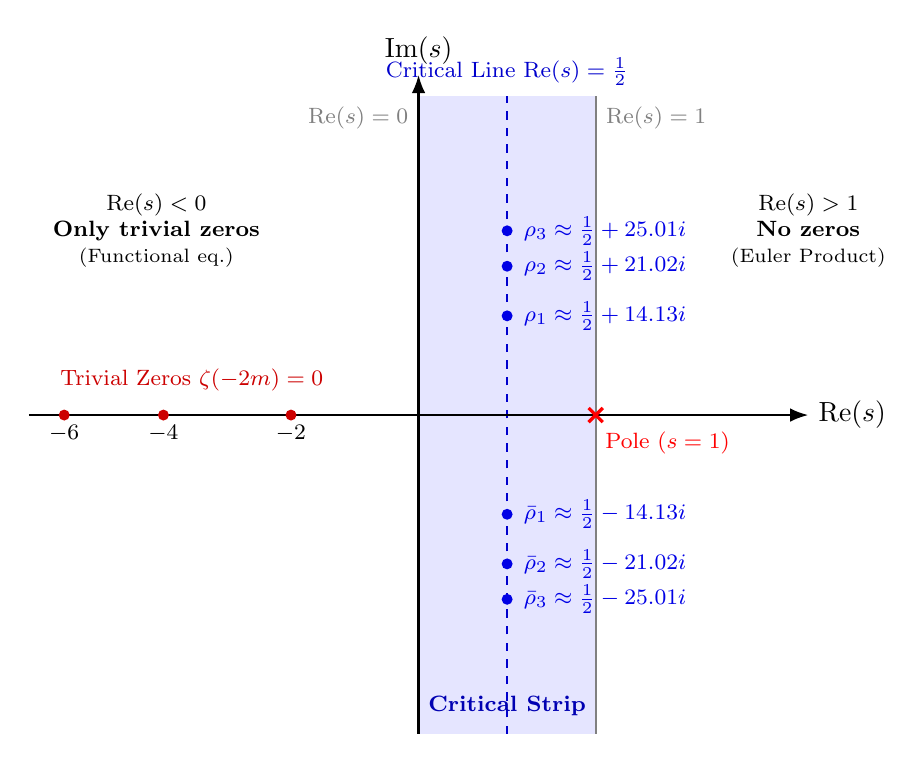
\begin{tikzpicture}[scale=0.9, >=Latex]
    % Critical strip shading
    \fill[blue!10] (0, -4.5) rectangle (2.5, 4.5);
    
    % Boundaries of critical strip
    \draw[thick, gray] (0, -4.5) -- (0, 4.5) node[below left, font=\footnotesize] {$\operatorname{Re}(s) = 0$};
    \draw[thick, gray] (2.5, -4.5) -- (2.5, 4.5) node[below right, font=\footnotesize] {$\operatorname{Re}(s) = 1$};
    
    % Critical line
    \draw[thick, blue!80!black, dashed] (1.25, -4.5) -- (1.25, 4.5) node[above, font=\footnotesize] {Critical Line $\operatorname{Re}(s) = \frac{1}{2}$};
    
    % Axes
    \draw[->, thick] (-5.5, 0) -- (5.5, 0) node[right] {$\operatorname{Re}(s)$};
    \draw[->, thick] (0, -4.5) -- (0, 4.8) node[above] {$\operatorname{Im}(s)$};
    
    % Simple pole at s = 1
    \draw[red, very thick] (2.4, -0.1) -- (2.6, 0.1);
    \draw[red, very thick] (2.4, 0.1) -- (2.6, -0.1);
    \node[red, below right, font=\footnotesize] at (2.5, -0.1) {Pole ($s=1$)};
    
    % Trivial zeros on negative real axis
    \fill[red!80!black] (-1.8, 0) circle (2.2pt);
    \fill[red!80!black] (-3.6, 0) circle (2.2pt);
    \fill[red!80!black] (-5.0, 0) circle (2.2pt);
    \node[below, font=\footnotesize] at (-1.8, 0) {$-2$};
    \node[below, font=\footnotesize] at (-3.6, 0) {$-4$};
    \node[below, font=\footnotesize] at (-5.0, 0) {$-6$};
    \node[above, red!80!black, font=\footnotesize] at (-3.2, 0.2) {Trivial Zeros $\zeta(-2m) = 0$};
    
    % Non-trivial zeros on the critical line
    \fill[blue!90!black] (1.25, 1.4) circle (2.2pt);
    \fill[blue!90!black] (1.25, -1.4) circle (2.2pt);
    \fill[blue!90!black] (1.25, 2.1) circle (2.2pt);
    \fill[blue!90!black] (1.25, -2.1) circle (2.2pt);
    \fill[blue!90!black] (1.25, 2.6) circle (2.2pt);
    \fill[blue!90!black] (1.25, -2.6) circle (2.2pt);
    
    \node[right, blue!90!black, font=\footnotesize] at (1.35, 1.4) {$\rho_1 \approx \frac{1}{2} + 14.13 i$};
    \node[right, blue!90!black, font=\footnotesize] at (1.35, -1.4) {$\bar{\rho}_1 \approx \frac{1}{2} - 14.13 i$};
    \node[right, blue!90!black, font=\footnotesize] at (1.35, 2.1) {$\rho_2 \approx \frac{1}{2} + 21.02 i$};
    \node[right, blue!90!black, font=\footnotesize] at (1.35, -2.1) {$\bar{\rho}_2 \approx \frac{1}{2} - 21.02 i$};
    \node[right, blue!90!black, font=\footnotesize] at (1.35, 2.6) {$\rho_3 \approx \frac{1}{2} + 25.01 i$};
    \node[right, blue!90!black, font=\footnotesize] at (1.35, -2.6) {$\bar{\rho}_3 \approx \frac{1}{2} - 25.01 i$};
    
    % Annotations
    \node[align=center, font=\footnotesize, fill=white, inner sep=2pt] at (5.5, 2.6) {$\operatorname{Re}(s) > 1$\\\textbf{No zeros}\\\scriptsize(Euler Product)};
    \node[align=center, font=\footnotesize, fill=white, inner sep=2pt] at (-3.7, 2.6) {$\operatorname{Re}(s) < 0$\\\textbf{Only trivial zeros}\\\scriptsize(Functional eq.)};
    \node[blue!70!black, font=\bfseries\footnotesize] at (1.25, -4.1) {Critical Strip};
\end{tikzpicture}
\caption{The complex $s$-plane: trivial zeros on the negative real axis, the pole at $s=1$, the critical strip $0 < \operatorname{Re}(s) < 1$, and non-trivial zeros lying symmetrically on the critical line $\operatorname{Re}(s) = \frac{1}{2}$.}
\label{zf:fig:critical-strip}
\end{figure}

\subsection{The Riemann Xi Function and Critical Line Symmetry}\label{zf:subsec:xi-function}

To study the non-trivial zeros on the critical line, Riemann introduced the completed function $\xi(s)$ in his 1859 paper:
\begin{equation}
    \label{zf:eq:xi-definition}
    \xi(s) := \frac{1}{2} s(s-1) \pi^{-\frac{s}{2}} \Gamma\left(\frac{s}{2}\right) \zeta(s)
\end{equation}
The prefactor $\frac{1}{2} s(s-1)$ cancels the simple pole of $\zeta(s)$ at $s=1$ and the pole of $\Gamma(s/2)$ at $s=0$. Consequently, $\xi(s)$ is an \textbf{entire function} of order 1. 

From Theorem~\ref{zf:thm:symmetric-functional-equation}, $\xi(s)$ satisfies the perfect reflection symmetry:
\begin{equation}
    \label{zf:eq:xi-reflection}
    \xi(s) = \xi(1-s)
\end{equation}
Notice that the zeros of $\xi(s)$ are precisely the non-trivial zeros of $\zeta(s)$ (the trivial zeros are cancelled by the poles of $\Gamma(s/2)$).

\begin{theorem}[The Real-Valued Function $\Xi(t)$]\label{zf:thm:xi-real}
Parameterizing the critical line by $s = \frac{1}{2} + it$ for $t \in \mathbb{R}$, define:
\begin{equation}
    \label{zf:eq:xi-t-def}
    \Xi(t) := \xi\left(\frac{1}{2} + it\right)
\end{equation}
Then $\Xi(t)$ is an \textbf{even}, \textbf{purely real-valued} function for all real $t$:
\begin{equation*}
    \Xi(-t) = \Xi(t) \quad \text{and} \quad \Xi(t) \in \mathbb{R} \quad (\forall t \in \mathbb{R})
\end{equation*}
\end{theorem}

\begin{proof}
Using the functional equation $\xi(s) = \xi(1-s)$ with $s = \frac{1}{2} + it$:
\begin{equation*}
    \Xi(-t) = \xi\left(\frac{1}{2} - it\right) = \xi\left(1 - \left(\frac{1}{2} + it\right)\right) = \xi\left(\frac{1}{2} + it\right) = \Xi(t)
\end{equation*}
which proves that $\Xi(t)$ is an even function.

To prove that $\Xi(t)$ is real-valued, observe that for real $s$, $\zeta(s)$, $\Gamma(s/2)$, and $s(s-1)$ are all real. By the Schwarz reflection principle, $\overline{\xi(s)} = \xi(\bar{s})$ for all $s \in \mathbb{C}$. Evaluating at $s = \frac{1}{2} + it$:
\begin{equation*}
    \overline{\Xi(t)} = \overline{\xi\left(\frac{1}{2} + it\right)} = \xi\left(\overline{\frac{1}{2} + it}\right) = \xi\left(\frac{1}{2} - it\right) = \Xi(-t) = \Xi(t)
\end{equation*}
Since $\overline{\Xi(t)} = \Xi(t)$, $\Xi(t)$ must be real for all $t \in \mathbb{R}$.
\end{proof}

\begin{remark}[Significance for Zeros]
Theorem~\ref{zf:thm:xi-real} converts the two-dimensional problem of locating complex zeros of $\zeta(s)$ on the critical line into the one-dimensional problem of finding the \textbf{real roots of a real-valued curve} $\Xi(t)$.

In 1914, G. H. Hardy used this real-variable formulation to prove that $\Xi(t)$ changes sign infinitely many times, establishing:
\begin{quote}
\textit{\textbf{Hardy's Theorem (1914):} There are infinitely many non-trivial zeros of $\zeta(s)$ lying exactly on the critical line $\operatorname{Re}(s) = \frac{1}{2}$.}
\end{quote}
In 1989, J. B. Conrey proved that at least $40.77\%$ of all non-trivial zeros lie strictly on the critical line.
\end{remark}

\subsection{The Riemann Hypothesis}\label{zf:subsec:riemann-hypothesis-statement}

\begin{tcolorbox}[colback=blue!5!white,colframe=blue!75!black,title=\textbf{The Riemann Hypothesis (Bernhard Riemann, 1859)}]
All non-trivial zeros of the Riemann zeta function $\zeta(s)$ lie on the \textbf{critical line}:
\begin{equation}
    \boxed{\operatorname{Re}(s) = \frac{1}{2}}
\end{equation}
Equivalently, all roots of the Riemann $\Xi$-function $\Xi(t)$ are purely real:
\begin{equation}
    \Xi(t) = 0 \implies t \in \mathbb{R}
\end{equation}
\end{tcolorbox}

The first five non-trivial zeros on the critical line have imaginary parts:
\begin{align*}
    \rho_1 &= \frac{1}{2} + i \cdot 14.13472514\dots \\
    \rho_2 &= \frac{1}{2} + i \cdot 21.02203964\dots \\
    \rho_3 &= \frac{1}{2} + i \cdot 25.01085758\dots \\
    \rho_4 &= \frac{1}{2} + i \cdot 30.42487613\dots \\
    \rho_5 &= \frac{1}{2} + i \cdot 32.93506159\dots
\end{align*}
To date, more than $10^{13}$ non-trivial zeros have been checked by computer algorithms, and every single one lies precisely on the critical line $\operatorname{Re}(s) = 1/2$. A general mathematical proof remains the most celebrated open problem in mathematics and is designated as a Clay Millennium Prize Problem.

\subsection{The ``Music of the Primes'': Riemann's Explicit Formula}\label{zf:subsec:music-of-primes}

Riemann's ultimate goal in studying $\zeta(s)$ was to understand the distribution of prime numbers with exact precision.

\subsubsection{Von Mangoldt and Chebyshev Functions}
To link primes with analytic continuation, define the \textbf{von Mangoldt function}:
\begin{equation}
    \Lambda(n) = \begin{cases}
        \ln p & \text{if } n = p^k \text{ for some prime } p \text{ and integer } k \ge 1 \\
        0 & \text{otherwise}
    \end{cases}
\end{equation}
Taking the logarithmic derivative of the Euler product (Theorem~\ref{zf:thm:euler-product}):
\begin{align*}
    \ln \zeta(s) &= - \sum_{p} \ln(1 - p^{-s}) \\
    -\frac{\zeta'(s)}{\zeta(s)} &= \sum_{p} \frac{p^{-s} \ln p}{1 - p^{-s}} = \sum_{p} \sum_{k=1}^\infty (\ln p) \, p^{-k s} = \sum_{n=1}^\infty \frac{\Lambda(n)}{n^s}
\end{align*}
The cumulative sum $\psi(x) = \sum_{n \le x} \Lambda(n)$ is \textbf{Chebyshev's second function}. Counting primes via $\psi(x)$ is weighted by $\ln p$, giving $\psi(x) \approx \sum_{p \le x} \ln p \approx \pi(x) \ln x$.

\subsubsection{Riemann's Explicit Formula}
By applying Perron's contour inversion formula to $-\frac{\zeta'(s)}{\zeta(s)}$ and evaluating the residues at the simple pole $s=1$, the trivial zeros, and the non-trivial zeros $\rho$, Riemann derived his celebrated \textbf{Explicit Formula}:

\begin{theorem}[Riemann's Explicit Formula]\label{zf:thm:explicit-formula}
For any non-integer $x > 1$:
\begin{equation}
    \label{zf:eq:explicit-formula}
    \boxed{
        \psi(x) = x - \sum_{\rho} \frac{x^\rho}{\rho} - \ln(2\pi) - \frac{1}{2} \ln(1 - x^{-2})
    }
\end{equation}
where the sum ranges over all non-trivial zeros $\rho = \beta + i\gamma$ of $\zeta(s)$, paired as $\lim_{T \to \infty} \sum_{|\gamma| < T} \frac{x^\rho}{\rho}$.
\end{theorem}

\subsubsection{The Harmonic Interpretation}
Writing each non-trivial zero as $\rho = \beta + i \gamma$:
\begin{equation}
    x^\rho = x^{\beta + i \gamma} = x^\beta e^{i \gamma \ln x} = x^\beta \left[ \cos(\gamma \ln x) + i \sin(\gamma \ln x) \right]
\end{equation}
Pairing conjugate zeros $\rho = \beta + i \gamma$ and $\bar{\rho} = \beta - i \gamma$ produces real oscillating harmonics:
\begin{equation*}
    \frac{x^\rho}{\rho} + \frac{x^{\bar{\rho}}}{\bar{\rho}} = 2 \operatorname{Re}\left( \frac{x^{\beta + i\gamma}}{\beta + i\gamma} \right) = \frac{2 x^\beta}{|\rho|} \cos\left( \gamma \ln x - \arg(\rho) \right)
\end{equation*}
Equation~\eqref{zf:eq:explicit-formula} decomposes the prime distribution into:
\begin{enumerate}[label=\arabic*.]
    \item \textbf{The Baseline Trend $x$}: Produced by the residue at the pole $s = 1$. This corresponds to the smooth asymptotic distribution of primes $\psi(x) \sim x$ (the Prime Number Theorem).
    \item \textbf{The Harmonic Oscillations $-\sum_\rho \frac{x^\rho}{\rho}$}: Each non-trivial zero $\rho$ contributes a pure wave with frequency $\frac{\gamma}{2\pi}$ on a logarithmic scale $\ln x$. The primes are literally the \textbf{constructive interference} of these infinite waves!
    \item \textbf{The Smooth Tail $-\ln(2\pi) - \frac{1}{2}\ln(1-x^{-2})$}: Produced by the residues at the trivial zeros $s = -2, -4, \dots$ and $s = 0$.
\end{enumerate}

\subsubsection{The Optimal Error Bound}
The real part $\beta = \operatorname{Re}(\rho)$ controls the \textbf{amplitude} of the prime fluctuations ($x^\beta$). 
\begin{itemize}
    \item If any zero had $\beta > 1/2$, the fluctuations would blow up with amplitude $x^\beta$, creating massive, irregular swings in prime density.
    \item Under the \textbf{Riemann Hypothesis}, all zeros have $\beta = 1/2$, making every oscillation have amplitude exactly $\sqrt{x}$.
\end{itemize}
This establishes the ultimate equivalence:
\begin{theorem}[Equivalence with the Prime Error Bound]
The Riemann Hypothesis is mathematically equivalent to the sharpest possible error bound for prime counting:
\begin{equation}
    \label{zf:eq:pnt-rh-error}
    \boxed{
        \pi(x) = \operatorname{Li}(x) + O\left(\sqrt{x} \ln x\right)
    }
\end{equation}
where $\operatorname{Li}(x) = \int_2^x \frac{dt}{\ln t}$ is the logarithmic integral.
\end{theorem}
The error $O(\sqrt{x} \ln x)$ is identical to the statistical fluctuation of an unbiased random walk of size $x$. Thus, the Riemann Hypothesis asserts that prime numbers are distributed with the maximum possible regularity permitted by arithmetic.

\end{document}

\clearpage

\documentclass[a4paper]{article}

% Shared Preamble for MathLatexDocs

% --- Core Packages ---
\usepackage[english]{babel}
\usepackage[utf8]{inputenc}
\usepackage{amsmath}
\usepackage{amsthm}
\usepackage{amssymb}
\usepackage{mathtools}
\usepackage{graphicx}
\usepackage{microtype} % Better justification and fewer overfull hboxes
\usepackage{bm}
\usepackage{enumitem}
\usepackage{booktabs}
\usepackage{mathrsfs}

% --- Layout & Design ---
\usepackage{docmute}
\usepackage{subfiles} % Support for master/subfile structure
\usepackage[colorinlistoftodos]{todonotes}
\usepackage[colorlinks=true, linkcolor=blue, citecolor=magenta]{hyperref}
\usepackage{cleveref} % Better cross-referencing
\usepackage{tcolorbox} % For styled boxes
\usepackage{tikz} % For drawing diagrams
\usetikzlibrary{arrows.meta,positioning}

% --- Theorem Environments (Classic Style) ---
\makeatletter
\@ifundefined{classicthm}{%
  \newtheorem{classicthm}{Theorem}[section]
  \newtheorem{classicdef}[classicthm]{Definition}
  \newtheorem{classiclem}[classicthm]{Lemma}
  \newtheorem{theorem}{Theorem}[section]
  \newtheorem{corollary}{Corollary}[theorem]
  \newtheorem{lemma}[theorem]{Lemma}
  \newtheorem{definition}{Definition}[section]
  \newtheorem{proposition}[theorem]{Proposition}
  \newtheorem{remark}[theorem]{Remark}
  \newtheorem{example}[theorem]{Example}
}{}

% Wrappers to maintain compatibility with the {Title}{Label} syntax used in files
\@ifundefined{mytheorem}{%
  \newenvironment{mytheorem}[2]{%
    \begin{classicthm}[#1]\label{thm:#2}
  }{%
    \end{classicthm}
  }
  
  \newenvironment{mydefinition}[2]{%
    \begin{classicdef}[#1]\label{def:#2}
  }{%
    \end{classicdef}
  }
  
  \newenvironment{mylemma}[2]{%
    \begin{classiclem}[#1]\label{lem:#2}
  }{%
    \end{classiclem}
  }
}{}
\makeatother

% --- Custom Commands ---
\providecommand{\Z}{\mathbb{Z}}
\providecommand{\R}{\mathbb{R}}
\providecommand{\C}{\mathbb{C}}
\providecommand{\N}{\mathbb{N}}
\providecommand{\G}{\mathcal{G}}
\providecommand{\Lop}{\mathcal{L}}
\providecommand{\PP}{\mathcal{P}}
\providecommand{\dd}{\,\mathrm{d}}
\providecommand{\bitand}{\mathbin{\&}}
\providecommand{\CFDots}{\genfrac{}{}{0pt}{0}{}{\ddots}}


\title{Integral Representation of Zeta(2)}
\author{Emil Kerimov}
\date{\today}

\begin{document}
\maketitle


\section{Integral Representation of Zeta(2)}\label{iz2:Integral Representation of Zeta(2)} 

$$
\int_{0}^{\infty}\frac{t}{e^{\alpha t}-1}dt
=\int_{0}^{\infty}\frac{te^{-\alpha t}}{1-e^{-\alpha t}}dt 
= \int_{0}^{\infty} t\sum\limits_{n=1}^{\infty} e^{-n\alpha t}dt
$$

By the Dominant Convergence Theorem: (Include Reference)

$$ \int_{0}^{\infty} t\sum\limits_{n=1}^{\infty} e^{-n\alpha t} dt
=\sum\limits_{n=1}^{\infty} \int_{0}^{\infty}  te^{-n\alpha t}dt$$

Using  $n\cdot \alpha \cdot t = x  \rightarrow n\cdot \alpha \cdot dt = dx$ 
$$
\sum\limits_{n=1}^{\infty} \int_{0}^{\infty}  \frac{x}{n\alpha}e^{-x}\frac{dx}{n\alpha}
=\sum\limits_{n=1}^{\infty} \frac{1}{n^2 \alpha^2 }\int_{0}^{\infty}  xe^{-x}dx
=\frac{1}{\alpha^2}\sum\limits_{n=1}^{\infty} \frac{1}{n^2}\Gamma(2)
$$

Recall $\Gamma(2) = 1! = 1$ (Include Reference)

$$\frac{1}{\alpha^2}\sum\limits_{n=1}^{\infty} \frac{1}{n^2}\Gamma(2)
=\frac{1}{\alpha^2}\sum\limits_{n=1}^{\infty} \frac{1}{n^2}
= \frac{1}{\alpha^2} \zeta(2)
$$

Recall $\zeta(2) = \frac{\pi^2}{6}$ (Include Reference)

$$
=>   \int_{0}^{\infty}\frac{t}{e^{\alpha t}-1}dt
=\frac{\pi^2}{6\alpha^2}
$$

\end{document}

\clearpage

\documentclass[a4paper]{article}

% Shared Preamble for MathLatexDocs

% --- Core Packages ---
\usepackage[english]{babel}
\usepackage[utf8]{inputenc}
\usepackage{amsmath}
\usepackage{amsthm}
\usepackage{amssymb}
\usepackage{mathtools}
\usepackage{graphicx}
\usepackage{microtype} % Better justification and fewer overfull hboxes
\usepackage{bm}
\usepackage{enumitem}
\usepackage{booktabs}
\usepackage{mathrsfs}

% --- Layout & Design ---
\usepackage{docmute}
\usepackage{subfiles} % Support for master/subfile structure
\usepackage[colorinlistoftodos]{todonotes}
\usepackage[colorlinks=true, linkcolor=blue, citecolor=magenta]{hyperref}
\usepackage{cleveref} % Better cross-referencing
\usepackage{tcolorbox} % For styled boxes
\usepackage{tikz} % For drawing diagrams
\usetikzlibrary{arrows.meta,positioning}

% --- Theorem Environments (Classic Style) ---
\makeatletter
\@ifundefined{classicthm}{%
  \newtheorem{classicthm}{Theorem}[section]
  \newtheorem{classicdef}[classicthm]{Definition}
  \newtheorem{classiclem}[classicthm]{Lemma}
  \newtheorem{theorem}{Theorem}[section]
  \newtheorem{corollary}{Corollary}[theorem]
  \newtheorem{lemma}[theorem]{Lemma}
  \newtheorem{definition}{Definition}[section]
  \newtheorem{proposition}[theorem]{Proposition}
  \newtheorem{remark}[theorem]{Remark}
  \newtheorem{example}[theorem]{Example}
}{}

% Wrappers to maintain compatibility with the {Title}{Label} syntax used in files
\@ifundefined{mytheorem}{%
  \newenvironment{mytheorem}[2]{%
    \begin{classicthm}[#1]\label{thm:#2}
  }{%
    \end{classicthm}
  }
  
  \newenvironment{mydefinition}[2]{%
    \begin{classicdef}[#1]\label{def:#2}
  }{%
    \end{classicdef}
  }
  
  \newenvironment{mylemma}[2]{%
    \begin{classiclem}[#1]\label{lem:#2}
  }{%
    \end{classiclem}
  }
}{}
\makeatother

% --- Custom Commands ---
\providecommand{\Z}{\mathbb{Z}}
\providecommand{\R}{\mathbb{R}}
\providecommand{\C}{\mathbb{C}}
\providecommand{\N}{\mathbb{N}}
\providecommand{\G}{\mathcal{G}}
\providecommand{\Lop}{\mathcal{L}}
\providecommand{\PP}{\mathcal{P}}
\providecommand{\dd}{\,\mathrm{d}}
\providecommand{\bitand}{\mathbin{\&}}
\providecommand{\CFDots}{\genfrac{}{}{0pt}{0}{}{\ddots}}


\title{Euler Sine Product Formula}
\author{Emil Kerimov}
\date{\today}
\begin{document}
\maketitle



\section{Sine Product Formula}

\begin{theorem} \label{spf:sine prod formula} 
$\boxed{\frac{sin(x)}{x} = \prod_{k=1}^{\infty} \Big( 1-\frac{x^2}{(k\pi)^2} \Big)}$

Proof
\begin{gather*}
\frac{sin(x)}{x} \text{has roots } x = \pi, -\pi, 2\pi, -2\pi, 3\pi, -3\pi, ... \\
\text{If we treat it as a normal polynomial then it can be written as a product of it's roots like such }\\
\frac{sin(x)}{x} = A \Big(1-\frac{x}{\pi}\Big)\Big(1+\frac{x}{\pi}\Big)
\Big(1-\frac{x}{2\pi}\Big)
\Big(1+\frac{x}{2\pi}\Big)
\Big(1-\frac{x}{3\pi}\Big)
\Big(1+\frac{x}{3\pi}\Big) \cdot \cdot \cdot \\
\text{For justification of why we can do this, see section \ref{spf:rigour}}\\
\frac{sin(x)}{x} = A \Big(1-\frac{x^2}{\pi^2}\Big)
\Big(1-\frac{x^2}{2^2 \pi^2}\Big)
\Big(1-\frac{x^2}{3^2 \pi^2}\Big) \cdot \cdot \cdot \\
\frac{sin(x)}{x} = A \prod_{k=1}^{\infty}
\Big(1-\frac{x^2}{k^2 \pi^2}\Big)
\\
\text{Solving for } A:
\\
\text{From the taylor expansion }
sin(x) = x - \frac{x^3}{3!} + \frac{x^5}{5!} - \frac{x^7}{7!} + ... \\
\lim_{x \to 0} \frac{sin(x)}{x} = \lim_{x \to 0} \frac{x}{x} - \frac{x^2}{3!} + \frac{x^4}{5!} - \frac{x^6}{7!} + ... \\
\lim_{x \to 0} \frac{sin(x)}{x} = 1\\
 A = 1 \\
 \frac{sin(x)}{x} = \prod_{k=1}^{\infty}
\Big(1-\frac{x^2}{k^2 \pi^2}\Big)
\end{gather*}
\end{theorem}

\subsection{Change of variables of the Sine Product Formula}
\begin{theorem} \label{spf:sine prod formula no pi} 
$\boxed{\frac{sin(\pi x)}{\pi x} = \prod_{k=1}^{\infty} \Big( 1-\frac{x^2}{k^2} \Big)}$

Proof\\
Replace $x$ with $x'/\pi$ in Theorem \ref{spf:sine prod formula}
\end{theorem}


\subsection{Basel Problem}
\label{spf:basel}
\subsubsection{Context}
This product form of sine was originally developed by Euler to solve the Basel problem. 
\\
\\
The Basel problem was to determine what value the sum $\sum_{k=1}^{\infty} \frac{1}{k^2}$ converged to. Mathematicians at the time knew that this infinite sum converged due to the various convergence tests, but no one knew the exact value. 
\\
\\
Euler's solution to this open problem was one of the first of many solutions for him to gain a reputation in the international math community.
\\
\\
This problem would later be generalized as a particular value of the zeta function, $\zeta(z) = \sum_{k=1}^{\infty} \frac{1}{k^z}$. Riemann was the first to consider complex value of this function, and even today there is an open millennium prize problem revolving around the zeros of this function. 
\subsubsection{Solution}
\begin{theorem} 
$\boxed{\sum_{k=1}^{\infty} \frac{1}{k^2} =  \frac{\pi^2}{6}}$

Proof\\
\begin{gather*}
\text{Expanding the product form }
\\
\frac{sin(x)}{x} = \prod_{k=1}^{\infty} \Big( 1-\frac{x^2}{(k\pi)^2} \Big) 
\\
\frac{sin(x)}{x} = 1 - \Big( \sum_{k=1}^{\infty} \frac{1}{k^2 \pi^2} \Big) x^2 + O\Big( x^4 \Big)
\\
\text{Expanding using the taylor series }\\
sin(x) = x - \frac{x^3}{3!} + \frac{x^5}{5!} - \frac{x^7}{7!} + ... 
\\
\text{Comparing the coefficient of } x^2 
\\
\sum_{k=1}^{\infty} \frac{1}{k^2 \pi^2} = \frac{1}{3!}
\\
\sum_{k=1}^{\infty} \frac{1}{k^2} = \frac{\pi^2}{6}
\end{gather*}
\end{theorem}


\subsection{Series representation of $cot(\pi x)$}
\begin{theorem} 
$\boxed{ \pi cot(\pi x) = \sum_{k=-\infty}^{\infty} \frac{1}{x + k} 
}$

Proof\\
\begin{gather*}
\text{Starting from Theorem \ref{spf:sine prod formula no pi}}
\\
\frac{sin(\pi x)}{\pi x} = \prod_{k=1}^{\infty} \Big( 1-\frac{x^2}{k^2} \Big)
\\
\intertext{The idea is to take the derivative of the log of both sides. \footnotemark}
\text{First taking the log of both sides}
\\
ln(sin(\pi x)) = ln(\pi x) + \sum_{k=1}^{\infty} ln \Big( 1-\frac{x^2}{k^2} \Big)
\\
\text{Now taking the derivative of both sides w.r.t. $x$ we get}
\\
\pi \frac{cos(\pi x)}{sin(\pi x)} = \frac{1}{x} + \sum_{k=1}^{\infty} \frac{\frac{-2x}{k^2}}{\Big( 1-\frac{x^2}{k^2} \Big)} 
\\
\intertext{Simplifying} 
\pi \cdot cot(\pi x) = \frac{1}{x} 
+ 2x \sum_{k=1}^{\infty} \frac{1}{x^2-k^2}
\\
\text{Note   } \frac{1}{x+k} + \frac{1}{x-k} = \frac{x-k + x+k}{x^2-k^2} = \frac{2x}{x^2-k^2}
\\
\intertext{Plugging this into the series expression} 
\pi \cdot cot(\pi x) = \frac{1}{x} 
+ \sum_{k=1}^{\infty} \frac{1}{x+k} + \frac{1}{x-k}
\\
\intertext{Cleaning up the indicies}
\pi \cdot cot(\pi x) = \sum_{k=-\infty}^{\infty} \frac{1}{x+k}
\end{gather*}
\end{theorem}

\footnotetext{This is similar to the definition of the Di-Gamma function $\Psi$, see Gamma function document.}


\begin{theorem} \label{spf:cot series zeta}
$\boxed{x \pi \cot(\pi x) = 1 - 2 \sum_{k=1}^{\infty} \zeta(2k) x^{2k}
}$

Proof\\
\begin{gather*}
\text{Starting from previous intermediate result}
\\
\pi cot(\pi x) = \frac{1}{x} + \sum_{k=1}^{\infty} \frac{\frac{-2x}{k^2}}{\Big( 1-\frac{x^2}{k^2} \Big)} 
\\
\pi x \cdot cot(\pi x) = 1 + \sum_{k=1}^{\infty} \frac{\frac{-2x^2}{k^2}}{\Big( 1-\frac{x^2}{k^2} \Big)} 
\\
\intertext{Using the infinite geometric series formula $\frac{1}{1-x} = \sum_{n=0}^{\infty} x^n $ for $|x| < 1$}
\pi x \cdot cot(\pi x) = 1 + \sum_{k=1}^{\infty} \Bigg( \sum_{n=0}^{\infty} \Big( \frac{x^2}{k^2} \Big)^n \Bigg) \frac{-2x^2}{k^2}  
\\
\intertext{Simplfying}
\pi x \cdot cot(\pi x) = 1 - 2 \sum_{k=1}^{\infty} \Bigg( \sum_{n=0}^{\infty} \Big( \frac{x^2}{k^2} \Big)^{n+1} \Bigg)
\\
\pi x \cdot cot(\pi x) = 1 - 2 \sum_{k=1}^{\infty} \Bigg( \sum_{n=1}^{\infty} \Big( \frac{x}{k} \Big)^{2n} \Bigg)
\\
\intertext{Interchanging the summations since both series are absolutly convergent \footnotemark}
\pi x \cdot cot(\pi x) = 1 - 2 \sum_{n=1}^{\infty} \Bigg( \sum_{k=1}^{\infty} \Big( \frac{1}{k^{2n}} \Big) \Bigg) x^{2n}
\\
\intertext{Using the definition of $\zeta(x) = \sum_{k=1}^{\infty} \frac{1}{k^x}$}
\pi x \cdot cot(\pi x) = 1 - 2 \sum_{n=1}^{\infty} \zeta(2n) x^{2n}
\end{gather*}
\end{theorem}

\footnotetext{Technically this needs to be shown.}


\subsection{Wallis Product}
\label{spf:wallis product}
\begin{theorem} 
$\boxed{ 
\prod_{n=1}^{\infty} \Big( \frac{2n}{2n-1} \Big) \Big( \frac{2n}{2n+1} \Big) = \frac{\pi}{2}
}$

Proof\\
\begin{gather*}
\text{Starting from Theorem \ref{spf:sine prod formula no pi}}
\\
\frac{sin(\pi x)}{\pi x} = \prod_{k=1}^{\infty} \Big( 1-\frac{x^2}{k^2} \Big)
\\
\intertext{Plugging in $x=\frac{1}{2}$}
\frac{sin(\frac{\pi}{2})}{\frac{\pi}{2}} = 
\frac{2}{\pi} = \prod_{k=1}^{\infty} \Big( 1-\frac{1}{4 k^2} \Big)
\\
\frac{2}{\pi} = \prod_{k=1}^{\infty} \Big( \frac{4 k^2 -1}{4 k^2} \Big)
\\
\frac{2}{\pi} = \prod_{k=1}^{\infty} \Big( \frac{2 k -1}{2 k} \Big) \cdot \Big( \frac{2 k +1}{2 k} \Big)
\\
\frac{\pi}{2} = \prod_{k=1}^{\infty} \Big( \frac{2k}{2 k -1} \Big) \cdot \Big( \frac{2 k }{2 k+1} \Big)
\end{gather*}
\end{theorem}



\section{Rigorous Convergence via Weierstrass Factorization}\label{spf:sec:convergence}
\label{spf:rigour}
Euler's original proof did not include proper justification of why we are allowed to write $\sin(x)$ as an infinite product of it's roots. The justification comes from what is known as Weierstrass factorization theorem. 

\subsection{Weierstrass factorization theorem}
Define elementary factors
\begin{equation}
E_{n}(z) = 
\begin{cases}
(1-z) &\text{if } n=0 \\
(1-z) e^{z + z^2/2 + ... + z^n /n} & otherwise 
\end{cases}
\end{equation}

\begin{theorem}
Let f be an entire function, and let $\{a_n\}$ be the non-zero zeros of f repeated according to multiplicity. Suppose also that f has a zero at z=0 of order m $\geq$ 0 (a zero of order m = 0 at z = 0 means $f(0) \not = 0$). Then there exists an entire function g and a sequence of integers  $\{p_n\}$ such that
\begin{equation}
f(z) = z^m e^{g(z)} \prod_{n=1}^{\infty} E_{p_n}(\frac{z}{a_n})
\end{equation}



\begin{proof}
The proof proceeds in three main steps: establishing local estimates for the elementary factors, proving uniform convergence of the infinite product on compact sets, and showing that the quotient function is zero-free and thus the exponential of an entire function.

\paragraph{Step 1: Estimate for the elementary factors.}
For $|u| \leq \frac{1}{2}$, we use the principal branch of the complex logarithm $\log(1-u) = -\sum_{k=1}^{\infty} \frac{u^k}{k}$ to evaluate $E_p(u)$:
\begin{equation*}
\log E_p(u) = \log(1-u) + \sum_{k=1}^{p} \frac{u^k}{k} = -\sum_{k=p+1}^{\infty} \frac{u^k}{k}
\end{equation*}
Taking the absolute value and bounding the series geometrically:
\begin{align*}
|\log E_p(u)| &\leq \sum_{k=p+1}^{\infty} \frac{|u|^k}{k} \leq \frac{|u|^{p+1}}{p+1} \sum_{j=0}^{\infty} |u|^j \\
&\leq \frac{|u|^{p+1}}{p+1} \frac{1}{1 - 1/2} = \frac{2}{p+1} |u|^{p+1} \leq |u|^{p+1}
\end{align*}
Using the standard inequality $|e^w - 1| \leq |w| e^{|w|} \leq 2|w|$ for $|w| \leq 1$, setting $w = \log E_p(u)$ yields:
\begin{equation*}
|E_p(u) - 1| \leq 2 |u|^{p+1} \quad \text{for all } |u| \leq \frac{1}{2}
\end{equation*}

\paragraph{Step 2: Convergence of the canonical product.}
Since the zeros $\{a_n\}$ have no finite limit point, $|a_n| \to \infty$ as $n \to \infty$. We choose the sequence of non-negative integers $\{p_n\}$ such that for every $R > 0$:
\begin{equation*}
\sum_{n=1}^{\infty} \left( \frac{R}{|a_n|} \right)^{p_n + 1} < \infty
\end{equation*}
(For instance, simply setting $p_n = n$ always guarantees convergence, since $|a_n| \geq 2R$ for all sufficiently large $n$, giving $(R/|a_n|)^{n+1} \leq (1/2)^{n+1}$).

Let $R > 0$ be arbitrary, and consider the closed disk $|z| \leq R$. There exists an index $N$ such that $|a_n| \geq 2R$ for all $n \geq N$. For any $z$ with $|z| \leq R$ and $n \geq N$, we have $\left| \frac{z}{a_n} \right| \leq \frac{1}{2}$, so the Step 1 bound applies:
\begin{equation*}
\left| E_{p_n}\left( \frac{z}{a_n} \right) - 1 \right| \leq 2 \left| \frac{z}{a_n} \right|^{p_n + 1} \leq 2 \left( \frac{R}{|a_n|} \right)^{p_n + 1}
\end{equation*}
By the Weierstrass $M$-test, the series $\sum_{n=1}^{\infty} \left| E_{p_n}\left(\frac{z}{a_n}\right) - 1 \right|$ converges uniformly on $|z| \leq R$. 
A fundamental theorem on infinite products of holomorphic functions states that absolute and uniform convergence of $\sum |1 - f_n(z)|$ implies that the infinite product
\begin{equation*}
P(z) = \prod_{n=1}^{\infty} E_{p_n}\left( \frac{z}{a_n} \right)
\end{equation*}
converges uniformly on compact subsets of $\mathbb{C}$. Therefore, $P(z)$ is an entire function whose zeros are precisely the non-zero roots $\{a_n\}$, counting multiplicities.

\paragraph{Step 3: Quotient and existence of $g(z)$.}
Now consider the quotient function:
\begin{equation*}
h(z) = \frac{f(z)}{z^m P(z)}
\end{equation*}
At $z = 0$, the zero of order $m$ in $f(z)$ is canceled by $z^m$, so $h(z)$ has a removable singularity at the origin with $h(0) \neq 0$. At each $a_n$, the zero in $P(z)$ matches the zero in $f(z)$ in both location and multiplicity, so each $a_n$ is likewise a removable singularity. 

After removing these singularities, $h(z)$ is an entire function that has \textbf{no zeros anywhere} in the complex plane: $h(z) \neq 0$ for all $z \in \mathbb{C}$.

Because the complex plane $\mathbb{C}$ is simply connected and $h(z)$ is nowhere zero, the logarithmic derivative $\frac{h'(z)}{h(z)}$ is holomorphic on $\mathbb{C}$. We can define:
\begin{equation*}
g(z) = \log h(0) + \int_{0}^{z} \frac{h'(w)}{h(w)} \, dw
\end{equation*}
where the path of integration is any contour from $0$ to $z$. By Cauchy's theorem, $g(z)$ is a well-defined entire function. Differentiating $e^{-g(z)} h(z)$ shows:
\begin{align*}
\frac{d}{dz} \left( e^{-g(z)} h(z) \right) &= -g'(z) e^{-g(z)} h(z) + e^{-g(z)} h'(z) \\
&= e^{-g(z)} \left( - \frac{h'(z)}{h(z)} h(z) + h'(z) \right) = 0
\end{align*}
Thus $e^{-g(z)} h(z) = e^{-g(0)} h(0) = 1$, which proves $h(z) = e^{g(z)}$. 

Substituting this back gives:
\begin{equation*}
f(z) = z^m e^{g(z)} \prod_{n=1}^{\infty} E_{p_n}\left( \frac{z}{a_n} \right)
\end{equation*}
which completes the proof.
\end{proof}
\end{theorem}


\end{document}

\clearpage

\documentclass[a4paper]{article}

% Shared Preamble for MathLatexDocs

% --- Core Packages ---
\usepackage[english]{babel}
\usepackage[utf8]{inputenc}
\usepackage{amsmath}
\usepackage{amsthm}
\usepackage{amssymb}
\usepackage{mathtools}
\usepackage{graphicx}
\usepackage{microtype} % Better justification and fewer overfull hboxes
\usepackage{bm}
\usepackage{enumitem}
\usepackage{booktabs}
\usepackage{mathrsfs}

% --- Layout & Design ---
\usepackage{docmute}
\usepackage{subfiles} % Support for master/subfile structure
\usepackage[colorinlistoftodos]{todonotes}
\usepackage[colorlinks=true, linkcolor=blue, citecolor=magenta]{hyperref}
\usepackage{cleveref} % Better cross-referencing
\usepackage{tcolorbox} % For styled boxes
\usepackage{tikz} % For drawing diagrams
\usetikzlibrary{arrows.meta,positioning}

% --- Theorem Environments (Classic Style) ---
\makeatletter
\@ifundefined{classicthm}{%
  \newtheorem{classicthm}{Theorem}[section]
  \newtheorem{classicdef}[classicthm]{Definition}
  \newtheorem{classiclem}[classicthm]{Lemma}
  \newtheorem{theorem}{Theorem}[section]
  \newtheorem{corollary}{Corollary}[theorem]
  \newtheorem{lemma}[theorem]{Lemma}
  \newtheorem{definition}{Definition}[section]
  \newtheorem{proposition}[theorem]{Proposition}
  \newtheorem{remark}[theorem]{Remark}
  \newtheorem{example}[theorem]{Example}
}{}

% Wrappers to maintain compatibility with the {Title}{Label} syntax used in files
\@ifundefined{mytheorem}{%
  \newenvironment{mytheorem}[2]{%
    \begin{classicthm}[#1]\label{thm:#2}
  }{%
    \end{classicthm}
  }
  
  \newenvironment{mydefinition}[2]{%
    \begin{classicdef}[#1]\label{def:#2}
  }{%
    \end{classicdef}
  }
  
  \newenvironment{mylemma}[2]{%
    \begin{classiclem}[#1]\label{lem:#2}
  }{%
    \end{classiclem}
  }
}{}
\makeatother

% --- Custom Commands ---
\providecommand{\Z}{\mathbb{Z}}
\providecommand{\R}{\mathbb{R}}
\providecommand{\C}{\mathbb{C}}
\providecommand{\N}{\mathbb{N}}
\providecommand{\G}{\mathcal{G}}
\providecommand{\Lop}{\mathcal{L}}
\providecommand{\PP}{\mathcal{P}}
\providecommand{\dd}{\,\mathrm{d}}
\providecommand{\bitand}{\mathbin{\&}}
\providecommand{\CFDots}{\genfrac{}{}{0pt}{0}{}{\ddots}}


\title{Darboux's formula}
\author{Emil Kerimov}
\date{}
\begin{document}
\maketitle

\section{Darboux's formula}\label{dar:sec:darboux}

Let $\phi(t)$ be a polynomial of degree $n$ and $f(x)$ is an analytic function then,

\begin{theorem}\label{dar:thm:darboux}
    \begin{multline}
        \sum_{m=0}^{n} (-1)^m (z-a)^m \Big[ \phi^{(n-m)}(1) f^{(m)}(z)  - \phi^{(n-m)}(0) f^{(m)}(a) \Big]
        =
        \\
        (-1)^n (z-a)^{n+1} \int_{0}^{1} \phi(t) f^{(n+1)}\Big[a + t(z-a)\Big] dt
    \end{multline}

    Proof
    \begin{gather*}
        \intertext{For $n = 0$ we have $\phi(t) = c$ then}
        LHS_{0} = c \Big[ f(z)  - f(a) \Big]
        \\
        RHS_{0} = (z-a) \int_{0}^{1} c f^{(1)}\Big[a + t(z-a)\Big] dt
        \intertext{After a change of variables $u = a + t(z-a)$, $du = dt(z-a)$ we get}
        RHS_{0} = c \int_{a}^{z} f^{(1)}(u) du = c \Big[ f(u)\Big] \Biggr|_{u=a}^{u=z} = c \Big[  f(z) - f(a) \Big] = LHS_{0}
        \\
        \intertext{For $n > 0$}
        RHS_{n} = (-1)^n (z-a)^{n+1} \int_{0}^{1} \phi(t) f^{(n+1)}\Big[a + t(z-a)\Big] dt
        \\
        \intertext{Using integration by parts $\int_{t=0}^{1} uv' = uv \big |_{t=0}^{1} - \int_{t=0}^{1} u'v$, with $u = \phi(t)$, and $ v' = f^{(n+1)}(a + t(z-a))$}
        RHS_{n} = (-1)^{n} (z-a)^{n+1} \Bigg[
            \phi(t) \frac{f^{(n)}\Big[a + t(z-a)\Big]}{(z-a)} \Biggr|_{t=0}^{t=1}
            -
            \int_{0}^{1} \phi'(t) \frac{f^{(n)}\Big[a + t(z-a)\Big]}{(z-a)} dt
            \Bigg]
        \\
        \intertext{Evaluating the first definite integral and multipying by $(z-a)$}
        RHS_{n} = (-1)^{n} (z-a)^{n} \Bigg[
            \phi(1) f^{(n)}(z) - \phi(0) f^{(n)}(a)
            -
            \int_{0}^{1} \phi'(t) f^{(n)}\Big[a + t(z-a)\Big] dt
            \Bigg]
        \\
        \intertext{Moving the second integral out to it's own term}
        RHS_{n} = (-1)^{n} (z-a)^{n} \Bigg[
            \phi(1) f^{(n)}(z) - \phi(0) f^{(n)}(a) \Bigg]
        + (-1)^{n-1} (z-a)^{n}
        \int_{0}^{1} \phi'(t) f^{(n)}\Big[a + t(z-a)\Big] dt
        \intertext{Repeating the integration by parts process we get}
        RHS_{n} = (-1)^{n} (z-a)^{n} \Bigg[
            \phi(1) f^{(n)}(z) - \phi(0) f^{(n)}(a) \Bigg]
        \\
        +(-1)^{n-1} (z-a)^{n-1} \Bigg[
            \phi^{(1)}(1) f^{(n-1)}(z) - \phi^{(1)}(0) f^{(n-1)}(a) \Bigg]
        \\
        + (-1)^{n-2} (z-a)^{n-1}
        \int_{0}^{1} \phi^{(2)}(t) f^{(n-1)}\Big[a + t(z-a)\Big] dt
        \intertext{Repeating the integration by parts $n$-times until $\phi^{(n+1)}(t) = 0$ we get}
        RHS_{n} = \sum_{k=0}^{n} (-1)^{n-k} (z-a)^{n-k} \Bigg[
            \phi^{(k)}(1) f^{(n-k)}(z) - \phi^{(k)}(0) f^{(n-k)}(a) \Bigg]
        + 0
        \intertext{Changing the index of summation $m=n-k$}
        RHS_{n} = \sum_{m=0}^{n} (-1)^{m} (z-a)^{m} \Bigg[
            \phi^{(n-m)}(1) f^{(m)}(z) - \phi^{(n-m)}(0) f^{(m)}(a) \Bigg]
        \intertext{Therefore we get}
        \sum_{m=0}^{n} (-1)^m (z-a)^m \Big[ \phi^{(n-m)}(1) f^{(m)}(z)  - \phi^{(n-m)}(0) f^{(m)}(a) \Big]
        =
        \\
        (-1)^n (z-a)^{n+1} \int_{0}^{1} \phi(t) f^{(n+1)}\Big[a + t(z-a)\Big] dt
    \end{gather*}
\end{theorem}

\pagebreak

\section{Derivation of Taylor's Theorem via Darboux}\label{dar:sec:taylor}
Set $\phi(t) = (t-1)^n$ into Darnoux's formula to obtain Taylor's formula.

\begin{theorem}
    \begin{equation}\label{dar:Taylor's formula}
        \boxed{
            f(z) = \sum_{m=0}^{n} \frac{(z-a)^m f^{(m)}(a)}{m!} + (-1)^n \frac{(z-a)^{n+1}}{n!} \int_{0}^{1} (t-1)^n f^{(n+1)}\Big[a + t(z-a)\Big] dt
        }
    \end{equation}

    Proof
    \begin{gather*}
        \intertext{Starting from Darboux's formula \ref{dar:Darboux's formula}}
        \sum_{m=0}^{n} (-1)^m (z-a)^m \Big[ \phi^{(n-m)}(1) f^{(m)}(z)  - \phi^{(n-m)}(0) f^{(m)}(a) \Big]
        =
        \\
        (-1)^n (z-a)^{n+1} \int_{0}^{1} \phi(t) f^{(n+1)}\Big[a + t(z-a)\Big] dt
        \intertext{Setting $\phi(t) = (t-1)^n$, which is an n-degree polynomial}
        \intertext{Note that $\phi^{(k)}(t) = \frac{n!}{(n-k)!} (t-1)^{n-k}$ for $k\leq n$, therefore}
        \phi^{(k)}(0) =\frac{n!}{(n-k)!} (-1)^{n-k} \quad \text{for } k \leq n
        \\
        \phi^{(k)}(1) = 0 \quad \text{for } k < n
        \\
        \phi^{(n)}(1) = n!
        \\
        \sum_{m=1}^{n} (-1)^m (z-a)^m \Big[ 0 - \frac{n! (-1)^{m}}{(m)!} f^{(m)}(a) \Big] + (-1)^0 (z-a)^0 \Big[n! f^{(0)}(z) - n! f^{(0)}(a) \Big]
        \\
        =
        (-1)^n (z-a)^{n+1} \int_{0}^{1} (t-1)^n f^{(n+1)}\Big[a + t(z-a)\Big] dt
        \intertext{Simplfiying and dividing by $n!$}
        -\sum_{m=1}^{n} \frac{(z-a)^m}{m!} f^{(m)}(a) + \Big[ f(z) - f(a) \Big]
        \\
        =
        (-1)^n  \frac{(z-a)^{n+1}}{n!}  \int_{0}^{1} (t-1)^n f^{(n+1)}\Big[a + t(z-a)\Big] dt
        \intertext{Rearranging}
        f(z) = f(a) +
        \sum_{m=1}^{n} \frac{(z-a)^m}{m!} f^{(m)}(a) + (-1)^n \frac{(z-a)^{n+1}}{n!} \int_{0}^{1} (t-1)^n f^{(n+1)}\Big[a + t(z-a)\Big] dt
        \intertext{Adding the extra term into the summation to finish the proof}
        f(z) = \sum_{m=0}^{n} \frac{(z-a)^m}{m!} f^{(m)}(a) + (-1)^n \frac{(z-a)^{n+1}}{n!} \int_{0}^{1} (t-1)^n f^{(n+1)}\Big[a + t(z-a)\Big] dt
    \end{gather*}
\end{theorem}

\subsection{Infinite Series}

\begin{theorem}
    If $|f^{(k)}(x)| \leq M$ and $|z-a| \leq R \quad \forall x$ then
    \begin{equation}\label{dar:Taylor's Series}
        \boxed{
            f(z) = \sum_{m=0}^{\infty} \frac{(z-a)^m f^{(m)}(a)}{m!}
        }
    \end{equation}

    Proof
    \begin{gather*}
        \intertext{Starting from Taylor's formula \ref{dar:Taylor's formula} and taking the limit as $n$ approaches infinity}
        f(z) = \sum_{m=0}^{\infty} \frac{(z-a)^m f^{(m)}(a)}{m!} + \lim_{n \to \infty} (-1)^n \frac{(z-a)^{n+1}}{n!} \int_{0}^{1} (t-1)^n f^{(n+1)}\Big[a + t(z-a)\Big] dt
        \\
        \intertext{Define the remainder term, and then we will show that it converges to 0}
        R_n = (-1)^n \frac{(z-a)^{n+1}}{n!} \int_{0}^{1} (t-1)^n f^{(n+1)}\Big[a + t(z-a)\Big] dt
        \\
        |R_n| = \Big|(-1)^n \Big| \cdot \Big| \frac{(z-a)^{n+1}}{n!} \Big| \cdot \Big| \int_{0}^{1} (t-1)^n f^{(n+1)}\Big[a + t(z-a)\Big] dt \Big|
        \\
        |R_n| \leq \frac{|z-a|^{n+1}}{n!} \cdot \int_{0}^{1} \Big| (t-1)^n \Big| \cdot \Big| f^{(n+1)}\Big[a + t(z-a)\Big] \Big| dt
        \intertext{Using $|f^{(k)}(x)| \leq M$}
        |R_n| \leq \frac{|z-a|^{n+1}}{n!} \cdot \int_{0}^{1} |t-1|^n \cdot M  dt
        \intertext{Using $|z-a| \leq R$}
        |R_n| \leq \frac{R^{n+1} M}{n!} \cdot \int_{0}^{1} |t-1|^n dt
        \intertext{Note that between $0 \leq t \leq 1$, $|t-1| \leq 1$, therefore}
        |R_n| \leq \frac{R^{n+1} M}{n!}
        \intertext{Therefore since $M$ and $R$ are constant:}
        \lim_{n \to \infty} R_n \leq \lim_{n \to \infty} |R_n| \leq 0
        \intertext{Therefore}
        f(z) = \sum_{m=0}^{\infty} \frac{(z-a)^m f^{(m)}(a)}{m!}
    \end{gather*}
\end{theorem}

\pagebreak

\section{Derivation of the Euler--Maclaurin Formula via Darboux}\label{dar:sec:euler-maclaurin}
Set $\phi(t) = B_n(x)$ into Darnoux's formula to obtain the Euler-Maclaurin formula, where $B_n(x)$ is the Bernoulli polynomial\footnote{$B_{n}(x) = \sum_{k=0}^{n} {n \choose k} B_k x^{n-k}$. See the Bernoulli number document for the full definition.}.

\begin{theorem}
    For any analytical $g(x)$

    \begin{equation}
        \boxed{
            \begin{gathered}\label{dar:Euler-Maclaurin's formula}
                w \sum_{j=0}^{r-1} g(a+jw)  - \int_{x=a}^{a+rw} g(x) dx
                =
                \frac{w}{2} \Big( g(a) - g(a+rw) \Big)
                +
                \\
                \sum_{k=1}^{\lfloor n/2 \rfloor} \frac{w^{2k} B_{2k}}{(2k)!} \Big(g^{(2k-1)}(a+rw) - g^{(2k-1)}(a)\Big) + R_{n,r}
                \\
                R_{n,r} = \frac{(-1)^{n+1} w^{n+1}}{n!} \int_{0}^{r} B_n(\{t\}) f^{(n+1)}(a+tw) dt
            \end{gathered}
        }
    \end{equation}

    Proof
    \begin{gather*}
        \intertext{Starting from Darboux's formula \ref{dar:Darboux's formula}}
        \sum_{m=0}^{n} (-1)^m (z-a)^m \Big[ \phi^{(n-m)}(1) f^{(m)}(z)  - \phi^{(n-m)}(0) f^{(m)}(a) \Big]
        =
        \\
        (-1)^n (z-a)^{n+1} \int_{0}^{1} \phi(t) f^{(n+1)}\Big[a + t(z-a)\Big] dt
        \intertext{Setting $\phi(t) = B_n(t)$, which is an n-degree polynomial}
        \intertext{Note that $\phi^{(k)}(t) = \frac{n!}{(n-k)!} B_{n-k}(t)$ for $k\leq n$, therefore}
        \phi^{(k)}(0) = \phi^{(k)}(1) = \frac{n!}{(n-k)!} B_{n-k} \quad \text{for } k \leq n, k \neq 1
        \\
        \phi^{(1)}(0) = - \phi^{(1)}(1) = B_1
        \intertext{adjusting the indicies we get}
        \phi^{(n-m)}(0) = \phi^{(n-m)}(1) = \frac{n!}{m!} B_{m} \quad \text{for } n \geq m \geq 0, m \neq 1
        \\
        \phi^{(n-1)}(0) = B_1 = -\phi^{(n-1)}(1)
        \intertext{Plugging these values into Darboux's formula, and removing the first two terms we get}
        \sum_{m=2}^{n} (-1)^m (z-a)^m \Big[  \frac{n!}{m!} B_{m} f^{(m)}(z)  -  \frac{n!}{m!} B_{m} f^{(m)}(a) \Big]
        + n! B_0 \Big(f(z) - f(a) \Big)
        \\
        + (-1) n! (z-a) \Big( - B_{1} f^{'}(z) -  B_{1} f^{'}(a) \Big)
        =
        (-1)^n (z-a)^{n+1} \int_{0}^{1} B_n(t) f^{(n+1)}\Big[a + t(z-a)\Big] dt
        \intertext{simplfying}
        \sum_{m=2}^{n} \frac{(-1)^m (z-a)^m B_m}{m!} (f^{(m)}(z) - f^{(m)}(a))
        + B_0 \Big(f(z) - f(a) \Big)
        + (z-a) B_1 \Big( f^{'}(z) + f^{'}(a) \Big)
        =
        \\
        \frac{(-1)^n (z-a)^{n+1}}{n!} \int_{0}^{1} B_n(t) f^{(n+1)}\Big[a + t(z-a)\Big] dt
        \intertext{To simplify notation let us define $R_n^{a}$}
        R_n^{a} = \frac{(-1)^n (z-a)^{n+1}}{n!} \int_{0}^{1} B_n(t) f^{(n+1)}\Big[a + t(z-a)\Big] dt
        \intertext{Therefore we get}
        \sum_{m=2}^{n} \frac{(-1)^m (z-a)^m B_m}{m!} (f^{(m)}(z) - f^{(m)}(a)) + B_0 \Big(f(z) - f(a) \Big)
        + (z-a) B_1 \Big( f^{'}(z) + f^{'}(a) \Big)
        = R_n^{a}
        \intertext{Plugging in $B_0 =1$ and $B_1 = -\frac{1}{2}$}
        \sum_{m=2}^{n} \frac{(-1)^m (z-a)^m B_m}{m!} \Big(f^{(m)}(z) - f^{(m)}(a)\Big) + \Big(f(z) - f(a) \Big)
        - (z-a) \frac{1}{2} \Big( f^{'}(z) + f^{'}(a) \Big)
        = R_n^{a}
        \intertext{Adding $(z-a) f^{'}(a)$ to both sides and rearranging we get}
        (z-a) f^{'}(a) = f(z) - f(a)
        - \frac{(z-a)}{2} \Big( f^{'}(z) - f^{'}(a) \Big)
        +
        \sum_{m=2}^{n} \frac{(-1)^m (z-a)^m B_m}{m!} \Big(f^{(m)}(z) - f^{(m)}(a)\Big)
        - R_n^{a}
        \intertext{Define $w=z-a$ and $g(x) = f'(x)$ therefore we get}
        w g(a) = \int_{x=a}^{a+w} g(x) dx
        - \frac{w}{2} \Big( g(a+w) - g(a) \Big)
        +
        \sum_{m=2}^{n} \frac{(-1)^m w^m B_m}{m!} \Big(g^{(m-1)}(a+w) - g^{(m-1)}(a)\Big)
        - R_n^{a}
        \intertext{Allowing $a$ to be multiples of $w$, $a'= a + j w$ and summing over $i$ we get}
        \sum_{j=0}^{r-1} w g(a+jw) = \sum_{j=0}^{r-1} \int_{x=a+jw}^{a+(j+1)w} g(x) dx
        - \sum_{j=0}^{r-1} \frac{w}{2} \Big( g(a+(j+1)w) - g(a+jw) \Big)
        \\
        +
        \sum_{j=0}^{r-1} \sum_{m=2}^{n} \frac{(-1)^m w^m B_m}{m!} \Big(g^{(m-1)}(a+(j+1)w) - g^{(m-1)}(a+jw)\Big)
        - \sum_{j=0}^{r-1} R_n^{a+jw}
        \intertext{Simplyfying and evaluating the sums we get}
        w \sum_{j=0}^{r-1} g(a+jw) = \int_{x=a}^{a+rw} g(x) dx
        - \frac{w}{2} \Big( g(a+rw) - g(a) \Big)
        \\
        + \sum_{m=2}^{n} \frac{(-1)^m w^m B_m}{m!} \Big(g^{(m-1)}(a+rw) - g^{(m-1)}(a)\Big)
        - \sum_{j=0}^{r-1} R_n^{a+jw}
        \intertext{Rearranging}
        w \sum_{j=0}^{r-1} g(a+jw)  - \int_{x=a}^{a+rw} g(x) dx =
        \frac{w}{2} \Big( g(a) - g(a+rw) \Big)
        \\
        + \sum_{m=2}^{n} \frac{(-1)^m w^m B_m}{m!} \Big(g^{(m-1)}(a+rw) - g^{(m-1)}(a)\Big)
        - \sum_{j=0}^{r-1} R_n^{a+jw}
        \intertext{Using the fact that $B_{2n+1}=0, n\geq 1$ we can simplfy the sum using m = 2k}
        w \sum_{j=0}^{r-1} g(a+jw)  - \int_{x=a}^{a+rw} g(x) dx =
        \frac{w}{2} \Big( g(a) - g(a+rw) \Big)
        \\
        + \sum_{k=1}^{\lfloor n/2 \rfloor} \frac{w^{2k} B_{2k}}{(2k)!} \Big(g^{(2k-1)}(a+rw) - g^{(2k-1)}(a)\Big)
        - \sum_{j=0}^{r-1} R_n^{a+jw}
        \intertext{Recall the remainder term definition}
        R_n^{a} = \frac{(-1)^n (z-a)^{n+1}}{n!} \int_{0}^{1} B_n(t) f^{(n+1)}\Big[a + t(z-a)\Big] dt
        \intertext{Plugging in the definition of $w = (z-a)$ we get}
        R_n^{a} = \frac{(-1)^n w^{n+1}}{n!} \int_{0}^{1} B_n(t) f^{(n+1)}\Big[a + tw\Big] dt
        \intertext{Define the new remainder term}
        R_n = - \sum_{j=0}^{r-1} R_n^{a+jw}
        \intertext{Plug in the definition of $R_n^{a+jw}$ and simplfy}
        R_n = - \sum_{j=0}^{r-1} \frac{(-1)^n w^{n+1}}{n!} \int_{0}^{1} B_n(t) f^{(n+1)}(a+jw + tw) dt
        \intertext{Simplfy the remainder term using the fractional operator $\{x\}$}
        R_{n,r} = \frac{(-1)^{n+1} w^{n+1}}{n!} \int_{0}^{r} B_n(\{t\}) f^{(n+1)}(a+tw) dt
    \end{gather*}
\end{theorem}

\subsection{Infinite Series}
Note that as $n$ approaches infinity, the remainder term goes to 0.
\begin{theorem}
    If $|g^{(k)}(x)| \leq M \quad \forall x$ and $a, w, M$ finite then
    \begin{equation}\label{dar:Inifite Euler Mac's Series}
        \boxed{
            \lim_{n \to \infty} R_{n,r} = \lim_{n \to \infty} \frac{(-1)^{n+1} w^{n+1}}{n!} \int_{0}^{r} B_n(\{t\}) f^{(n+1)}(a+tw) dt = 0
        }
    \end{equation}

    Proof
    \begin{gather*}
        \intertext{Starting from the definition of $R_{n,r}$}
        \lim_{n \to \infty} R_n = \lim_{n \to \infty} \frac{(-1)^{n+1} w^{n+1}}{n!} \int_{0}^{r} B_n(\{t\}) f^{(n+1)}(a+tw) dt = 0
        \\
        \lim_{n \to \infty} R_n \leq \lim_{n \to \infty} |R_n|
        \\
        |R_n| \leq \frac{|w|^{n+1}}{n!} \int_{0}^{r} |B_n(\{t\})| M dt \leq \frac{|w|^{n+1} |B_n(t)| r M }{n!}
        \intertext{Using $\lim_{n \to \infty} \frac{B_n(x)}{n!} = 0$ from BERNOULLI DOCUMENT TODO}
        \lim_{n \to \infty} R_n \leq \lim_{n \to \infty} |R_n| = 0
    \end{gather*}

\end{theorem}


\subsection{Simple version}
By specifying $a=0$ and $w=1$ we obtain an exact difference between the summation and the integral of any analytic function $g(x)$.

\begin{theorem}
    For any analytical $g(x)$

    \begin{equation}
        \boxed{
            \begin{gathered}\label{dar:Simple Euler-Maclaurin's formula}
                \sum_{j=0}^{r} g(j)  - \int_{x=0}^{r} g(x) dx
                =
                \frac{g(0) + g(r)}{2} +
                \sum_{k=1}^{\lfloor n/2 \rfloor} \frac{B_{2k}}{(2k)!} \Big(g^{(2k-1)}(r) - g^{(2k-1)}(0)\Big) + R_{n, r}
                \\
                R_{n, r} = \frac{(-1)^{n+1} }{n!} \int_{0}^{r} B_n(\{t\}) g^{(n)}(t) dt
            \end{gathered}
        }
    \end{equation}

    Proof
    \begin{gather*}
        \intertext{Starting from the Euler-Maclaurin formula}
        w \sum_{j=0}^{r-1} g(a+jw)  - \int_{x=a}^{a+rw} g(x) dx
        =
        \frac{w}{2} \Big( g(a) - g(a+rw) \Big)
        +
        \\
        \sum_{k=1}^{\lfloor n/2 \rfloor} \frac{w^{2k} B_{2k}}{(2k)!} \Big(g^{(2k-1)}(a+rw) - g^{(2k-1)}(a)\Big) + R_{n, r}
        \\
        R_{n, r} = \frac{(-1)^{n+1} w^{n+1}}{n!} \int_{0}^{r} B_n(\{t\}) g^{(n)}(a+tw) dt
        \intertext{Plugging in $a=0$ and $w=1$ we get}
        \sum_{j=0}^{r-1} g(j)  - \int_{x=0}^{r} g(x) dx
        =
        \frac{1}{2} \Big( g(0) - g(r) \Big)
        +
        \sum_{k=1}^{\lfloor n/2 \rfloor} \frac{B_{2k}}{(2k)!} \Big(g^{(2k-1)}(r) - g^{(2k-1)}(0)\Big) + R_{n, r}
        \\
        R_{n, r} = \frac{(-1)^{n+1}}{n!} \int_{0}^{r} B_n(\{t\}) g^{(n)}(t) dt
        \intertext{Adding $g(r)$ to both sides}
        \sum_{j=0}^{r} g(j)  - \int_{x=0}^{r} g(x) dx
        =
        \frac{g(0) + g(r)}{2} +
        \sum_{k=1}^{\lfloor n/2 \rfloor} \frac{B_{2k}}{(2k)!} \Big(g^{(2k-1)}(r) - g^{(2k-1)}(0)\Big) + R_{n, r}
    \end{gather*}
\end{theorem}

\end{document}

\clearpage

\documentclass[a4paper]{article}

% Shared Preamble for MathLatexDocs

% --- Core Packages ---
\usepackage[english]{babel}
\usepackage[utf8]{inputenc}
\usepackage{amsmath}
\usepackage{amsthm}
\usepackage{amssymb}
\usepackage{mathtools}
\usepackage{graphicx}
\usepackage{microtype} % Better justification and fewer overfull hboxes
\usepackage{bm}
\usepackage{enumitem}
\usepackage{booktabs}
\usepackage{mathrsfs}

% --- Layout & Design ---
\usepackage{docmute}
\usepackage{subfiles} % Support for master/subfile structure
\usepackage[colorinlistoftodos]{todonotes}
\usepackage[colorlinks=true, linkcolor=blue, citecolor=magenta]{hyperref}
\usepackage{cleveref} % Better cross-referencing
\usepackage{tcolorbox} % For styled boxes
\usepackage{tikz} % For drawing diagrams
\usetikzlibrary{arrows.meta,positioning}

% --- Theorem Environments (Classic Style) ---
\makeatletter
\@ifundefined{classicthm}{%
  \newtheorem{classicthm}{Theorem}[section]
  \newtheorem{classicdef}[classicthm]{Definition}
  \newtheorem{classiclem}[classicthm]{Lemma}
  \newtheorem{theorem}{Theorem}[section]
  \newtheorem{corollary}{Corollary}[theorem]
  \newtheorem{lemma}[theorem]{Lemma}
  \newtheorem{definition}{Definition}[section]
  \newtheorem{proposition}[theorem]{Proposition}
  \newtheorem{remark}[theorem]{Remark}
  \newtheorem{example}[theorem]{Example}
}{}

% Wrappers to maintain compatibility with the {Title}{Label} syntax used in files
\@ifundefined{mytheorem}{%
  \newenvironment{mytheorem}[2]{%
    \begin{classicthm}[#1]\label{thm:#2}
  }{%
    \end{classicthm}
  }
  
  \newenvironment{mydefinition}[2]{%
    \begin{classicdef}[#1]\label{def:#2}
  }{%
    \end{classicdef}
  }
  
  \newenvironment{mylemma}[2]{%
    \begin{classiclem}[#1]\label{lem:#2}
  }{%
    \end{classiclem}
  }
}{}
\makeatother

% --- Custom Commands ---
\providecommand{\Z}{\mathbb{Z}}
\providecommand{\R}{\mathbb{R}}
\providecommand{\C}{\mathbb{C}}
\providecommand{\N}{\mathbb{N}}
\providecommand{\G}{\mathcal{G}}
\providecommand{\Lop}{\mathcal{L}}
\providecommand{\PP}{\mathcal{P}}
\providecommand{\dd}{\,\mathrm{d}}
\providecommand{\bitand}{\mathbin{\&}}
\providecommand{\CFDots}{\genfrac{}{}{0pt}{0}{}{\ddots}}


\title{Gaussian Integral}
\author{Emil Kerimov}
\date{\today}
\begin{document}
\maketitle

\section{Gaussian Integral} 

\begin{theorem}
$$
\int_{-\infty}^{\infty}{e^{-ax^2}}dx = \sqrt{\frac{\pi}{a}}
$$
Proof

\begin{gather*}
\shortintertext{Defining $I$}
I = \int_{-\infty}^{\infty}{e^{-ax^2}}dx\\
\shortintertext{Squaring $I$}
I^2 = \int_{-\infty}^{\infty}{e^{-ax^2}}dx \cdot \int_{-\infty}^{\infty}{e^{-ay^2}}dy\\
\shortintertext{Combining the integrals}
I^2 = \int_{-\infty}^{\infty} \int_{-\infty}^{\infty}{e^{-ax^2 - ay^2}}dx dy\\
\shortintertext{Converting to Polar coordinates}
I^2 = \int_{0}^{2 \pi} \int_{0}^{\infty}{e^{-ar^2}}rdr d\theta\\
\shortintertext{Solving}
\begin{alignedat}{2}
I^2 &= \int_{0}^{2 \pi} \tfrac{-1}{2a} e^{-ar^2} \Big|_0^{\infty} d\theta \\
I^2 &= \int_{0}^{2 \pi} \tfrac{1}{2a} d\theta \\
I^2 &= 2 \pi \tfrac{1}{2a} \\
I^2 &= \frac{\pi}{a} \\
I &= \sqrt{\frac{\pi}{a}} \\
\int_{-\infty}^{\infty}{e^{-ax^2}}dx &= \sqrt{\frac{\pi}{a}} \\
\end{alignedat}
\end{gather*}
\end{theorem}

Since $e^{-ax^2}$ is an even function we also get the integral
\begin{equation}
\int_{0}^{\infty}{e^{-ax^2}}dx = \frac{\sqrt{\frac{\pi}{a}}}{2} = \sqrt{\frac{\pi}{4a}} 
\end{equation}

\section{Higher Moments and Parameterized Gaussian Integrals}\label{gi:sec:parameterized-integrals} 
Using $
\int_{-\infty}^{\infty}{e^{-ax^2}}dx = \sqrt{\frac{\pi}{a}}
$ we can take derivatives with respect to (w.r.t.) $a$
 
\begin{gather*}
\frac{\partial}{\partial a} \int_{-\infty}^{\infty}{e^{-ax^2}}dx = \frac{\partial}{\partial a} \sqrt{\frac{\pi}{a}}  \\
\int_{-\infty}^{\infty}{-x^2 e^{-ax^2}}dx = \sqrt{\pi} \frac{-1}{2} a^{-3/2} \\
\boxed{
\int_{-\infty}^{\infty}{x^2 e^{-ax^2}}dx = \frac{1}{2a}  \sqrt{\frac{\pi}{a}}
}\\
\end{gather*}
This process can be repeated to obtain the general identity

\begin{equation}
\boxed{
\int_{-\infty}^{\infty}{x^{2n} e^{-ax^2}}dx = \frac{\pi}{|\Gamma(\tfrac{1}{2} - n)|a^n \sqrt{a}}}
\end{equation}

\end{document}

\clearpage

\documentclass[a4paper]{article}

% Shared Preamble for MathLatexDocs

% --- Core Packages ---
\usepackage[english]{babel}
\usepackage[utf8]{inputenc}
\usepackage{amsmath}
\usepackage{amsthm}
\usepackage{amssymb}
\usepackage{mathtools}
\usepackage{graphicx}
\usepackage{microtype} % Better justification and fewer overfull hboxes
\usepackage{bm}
\usepackage{enumitem}
\usepackage{booktabs}
\usepackage{mathrsfs}

% --- Layout & Design ---
\usepackage{docmute}
\usepackage{subfiles} % Support for master/subfile structure
\usepackage[colorinlistoftodos]{todonotes}
\usepackage[colorlinks=true, linkcolor=blue, citecolor=magenta]{hyperref}
\usepackage{cleveref} % Better cross-referencing
\usepackage{tcolorbox} % For styled boxes
\usepackage{tikz} % For drawing diagrams
\usetikzlibrary{arrows.meta,positioning}

% --- Theorem Environments (Classic Style) ---
\makeatletter
\@ifundefined{classicthm}{%
  \newtheorem{classicthm}{Theorem}[section]
  \newtheorem{classicdef}[classicthm]{Definition}
  \newtheorem{classiclem}[classicthm]{Lemma}
  \newtheorem{theorem}{Theorem}[section]
  \newtheorem{corollary}{Corollary}[theorem]
  \newtheorem{lemma}[theorem]{Lemma}
  \newtheorem{definition}{Definition}[section]
  \newtheorem{proposition}[theorem]{Proposition}
  \newtheorem{remark}[theorem]{Remark}
  \newtheorem{example}[theorem]{Example}
}{}

% Wrappers to maintain compatibility with the {Title}{Label} syntax used in files
\@ifundefined{mytheorem}{%
  \newenvironment{mytheorem}[2]{%
    \begin{classicthm}[#1]\label{thm:#2}
  }{%
    \end{classicthm}
  }
  
  \newenvironment{mydefinition}[2]{%
    \begin{classicdef}[#1]\label{def:#2}
  }{%
    \end{classicdef}
  }
  
  \newenvironment{mylemma}[2]{%
    \begin{classiclem}[#1]\label{lem:#2}
  }{%
    \end{classiclem}
  }
}{}
\makeatother

% --- Custom Commands ---
\providecommand{\Z}{\mathbb{Z}}
\providecommand{\R}{\mathbb{R}}
\providecommand{\C}{\mathbb{C}}
\providecommand{\N}{\mathbb{N}}
\providecommand{\G}{\mathcal{G}}
\providecommand{\Lop}{\mathcal{L}}
\providecommand{\PP}{\mathcal{P}}
\providecommand{\dd}{\,\mathrm{d}}
\providecommand{\bitand}{\mathbin{\&}}
\providecommand{\CFDots}{\genfrac{}{}{0pt}{0}{}{\ddots}}


\title{Properties of Fourier Series}
\author{Emil Kerimov}
\date{\today}

\begin{document}
\maketitle

\section{Properties of Fourier Series}\label{fs:fourier}
A function $f(x)$ can be written as the series shown in~\cref{fourier_series}, known as a Fourier Series. The following provides derivation of the properties of Fourier Series.

\begin{equation}\label{fs:fourier_series}
f(x) = a_0 + \sum\limits_{n=1}^{\infty} a_n cos(n x) + b_n sin(n x)
\end{equation}


\subsection{Trigonometric Addition Identities}\label{fs:trig_identities_addittion}
Recall equations~\cref{cos_a_plus_b,cos_a_minus_b,sin_a_plus_b,sin_a_minus_b}

\begin{equation}\label{fs:cos_a_plus_b}
cos(a+b) = cos(a) cos(b) - sin(a) sin(b)
\end{equation}
\begin{equation}\label{fs:cos_a_minus_b}
cos(a-b) = cos(a) cos(b) + sin(a) sin(b)
\end{equation}
\begin{equation}\label{fs:sin_a_plus_b}
sin(a+b) = sin(a) cos(b) + sin(b) cos(a)
\end{equation}
\begin{equation}\label{fs:sin_a_minus_b}
sin(a-b) = sin(a) cos(b) - sin(b) cos(b)
\end{equation}

From equations~\cref{cos_a_plus_b,cos_a_minus_b,sin_a_plus_b,sin_a_minus_b} we obtain ~\cref{cos_a_times_cos_b,sin_a_times_cos_b,sin_a_times_sin_b}

\begin{equation}\label{fs:cos_a_times_cos_b}
cos(a) cos(b) = \frac{1}{2} (cos(a+b) + cos(a-b))
\end{equation}
\begin{equation}\label{fs:sin_a_times_cos_b}
sin(a) cos(b)  = \frac{1}{2}(sin(a+b) + sin(a-b))
\end{equation}
\begin{equation}\label{fs:sin_a_times_sin_b}
sin(a) sin(b)  = \frac{1}{2}(cos(a-b) - cos(a+b))
\end{equation}

\subsection{Orthogonality Integrals}\label{fs:integrals}
Since $sin(n x)$ is an odd function, its integral  over a symmetric region is zero.
\begin{equation}\label{fs:int_sin_nx}
\int \limits_{-\pi}^{\pi} sin(n x) dx = 0
\end{equation}

Since $n$ is an integer, and assuming $n>0$, we obtain the following.
\begin{equation}\label{fs:int_cos_nx}
\int \limits_{-\pi}^{\pi} cos(n x) dx = \frac{2 sin(\pi n)}{n}=0
\end{equation}

Since $sin(m x) cos(n x)$ is an odd function, its integral  over a symmetric region is zero.
\begin{equation}\label{fs:int_sin_mx_cos_nx}
\int \limits_{-\pi}^{\pi} sin(m x) cos(n x) dx = 0
\end{equation}

Use~\cref{cos_a_times_cos_b} to write the following.
\begin{multline}\label{fs:int_cos_mx_cos_nx}
\int \limits_{-\pi}^{\pi} cos(m x) cos(n x) dx = 
\frac{1}{2} \int \limits_{-\pi}^{\pi} cos((n+m) x) dx + \frac{1}{2} \int \limits_{-\pi}^{\pi}
cos((n-m) x) dx \\
=\begin{cases} 0, & m \neq n \\ \pi, &m=n \end{cases}
\end{multline}

Using~\cref{sin_a_times_sin_b} we obtain the following.
\begin{multline}\label{fs:int_sin_mx_sin_nx}
\int \limits_{-\pi}^{\pi} sin(m x) sin(n x) dx
=\frac{1}{2} \int \limits_{-\pi}^{\pi} cos((n-m) x) dx - \frac{1}{2} \int \limits_{-\pi}^{\pi}
cos((n+m) x) dx \\
=\begin{cases} 0, & m \neq n \\ \pi, &m=n \end{cases}
\end{multline}


\subsection{$a_0$ Coefficient}\label{fs:a0_coefficient}
Integrate both sides of~\cref{fourier_series} to obtain:
$$\int \limits_{-\pi}^{\pi} f(x) dx = \int \limits_{-\pi}^{\pi} a_0 dx + \sum \limits_{n=1}^{\infty} (a_n \int \limits_{-\pi}^{\pi} cos(n x) dx + b_n \int \limits_{-\pi}^{\pi} sin(n x) dx)$$
Using \cref{int_sin_nx,int_cos_nx} the sum terms become zero.
$$=\int \limits_{-\pi}^{\pi} a_0 +0+0=a_0 x|_{-\pi}^{\pi}=a_0 \pi + a_0 \pi = 2\pi a_0$$
And thus we obtain
\begin{equation}\label{fs:a0}
a_0 = \frac{\int \limits_{-\pi}^{\pi} f(x) dx}{2\pi}
\end{equation}

\subsection{$a_n$ Coefficients}\label{fs:an_coefficient}
Multiply both sides of~\cref{fourier_series} by $cos(m x)$ to obtain:
$$f(x) cos(m x)= a_0 cos(m x) + \sum\limits_{n=1}^{\infty} a_n cos(n x) cos(m x) + b_n sin(n x) cos(m x)$$
Integrate both sides.
$$\int \limits_{-\pi}^{\pi}f(x) cos(m x) dx= a_0 \int \limits_{-\pi}^{\pi} cos(m x) dx 
+ \sum\limits_{n=1}^{\infty} (
a_n \int \limits_{-\pi}^{\pi}cos(n x) cos(m x) dx
+ b_n \int \limits_{-\pi}^{\pi} sin(n x) cos(m x) dx
)$$
$\rightarrow \int \limits_{-\pi}^{\pi} cos(m x) dx=0$ (from~\cref{int_cos_nx})\\
$\rightarrow \sum\limits_{n=1}^{\infty} (
a_n \int \limits_{-\pi}^{\pi}cos(n x) cos(m x) dx = \int \limits_{-\pi}^{\pi} a_m cos(m x) cos (m x) + \sum \limits_{n=1, n\neq m}^{\infty} \int \limits_{-\pi}^{\pi} cos(n x) cos(m x)$, which (from~\cref{int_cos_mx_cos_nx}) is equal to $a_m \pi + \sum \limits_{n=1, n\neq m}^{\infty} 0 = a_m \pi$.\\
$\rightarrow \int \limits_{-\pi}^{\pi} sin(n x) cos(m x) dx = 0$ (from~\cref{int_sin_mx_sin_nx}).
Thus we obtain:
$$\int \limits_{-\pi}^{\pi}f(x) cos(m x) dx = 0+a_m \pi + 0$$
And thus:
$$a_m = \frac{\int \limits_{-\pi}^{\pi} f(x) cos(m x) dx}{\pi}$$
Which, by changing the index from $m$ to $n$ gives:
\begin{equation}\label{fs:an}
a_n = \frac{\int \limits_{-\pi}^{\pi} f(x) cos(n x) dx}{\pi}
\end{equation}

\subsection{$b_n$ Coefficients}\label{fs:bn_coefficient}
Using similar arguments to~\cref{an_coefficient} we obtain:
\begin{equation}\label{fs:bn}
b_n = \frac{\int \limits_{-\pi}^{\pi} f(x) sin(n x) dx}{\pi}
\end{equation}

\end{document}

\clearpage

\documentclass[a4paper]{article}

% Shared Preamble for MathLatexDocs

% --- Core Packages ---
\usepackage[english]{babel}
\usepackage[utf8]{inputenc}
\usepackage{amsmath}
\usepackage{amsthm}
\usepackage{amssymb}
\usepackage{mathtools}
\usepackage{graphicx}
\usepackage{microtype} % Better justification and fewer overfull hboxes
\usepackage{bm}
\usepackage{enumitem}
\usepackage{booktabs}
\usepackage{mathrsfs}

% --- Layout & Design ---
\usepackage{docmute}
\usepackage{subfiles} % Support for master/subfile structure
\usepackage[colorinlistoftodos]{todonotes}
\usepackage[colorlinks=true, linkcolor=blue, citecolor=magenta]{hyperref}
\usepackage{cleveref} % Better cross-referencing
\usepackage{tcolorbox} % For styled boxes
\usepackage{tikz} % For drawing diagrams
\usetikzlibrary{arrows.meta,positioning}

% --- Theorem Environments (Classic Style) ---
\makeatletter
\@ifundefined{classicthm}{%
  \newtheorem{classicthm}{Theorem}[section]
  \newtheorem{classicdef}[classicthm]{Definition}
  \newtheorem{classiclem}[classicthm]{Lemma}
  \newtheorem{theorem}{Theorem}[section]
  \newtheorem{corollary}{Corollary}[theorem]
  \newtheorem{lemma}[theorem]{Lemma}
  \newtheorem{definition}{Definition}[section]
  \newtheorem{proposition}[theorem]{Proposition}
  \newtheorem{remark}[theorem]{Remark}
  \newtheorem{example}[theorem]{Example}
}{}

% Wrappers to maintain compatibility with the {Title}{Label} syntax used in files
\@ifundefined{mytheorem}{%
  \newenvironment{mytheorem}[2]{%
    \begin{classicthm}[#1]\label{thm:#2}
  }{%
    \end{classicthm}
  }
  
  \newenvironment{mydefinition}[2]{%
    \begin{classicdef}[#1]\label{def:#2}
  }{%
    \end{classicdef}
  }
  
  \newenvironment{mylemma}[2]{%
    \begin{classiclem}[#1]\label{lem:#2}
  }{%
    \end{classiclem}
  }
}{}
\makeatother

% --- Custom Commands ---
\providecommand{\Z}{\mathbb{Z}}
\providecommand{\R}{\mathbb{R}}
\providecommand{\C}{\mathbb{C}}
\providecommand{\N}{\mathbb{N}}
\providecommand{\G}{\mathcal{G}}
\providecommand{\Lop}{\mathcal{L}}
\providecommand{\PP}{\mathcal{P}}
\providecommand{\dd}{\,\mathrm{d}}
\providecommand{\bitand}{\mathbin{\&}}
\providecommand{\CFDots}{\genfrac{}{}{0pt}{0}{}{\ddots}}


\title{Useful Imaginary Identities}
\author{Emil Kerimov}
\date{\today}
\begin{document}
\maketitle





\section{The Imaginary Unit and Fundamental Identities}\label{uii:sec:definition}
Define a number $i$ such that 
\begin{definition} \label{uii:i def}
$$
\boxed{
i^2 = -1
}$$
\end{definition}

\section{Euler's equation}
This formula is the underlying connection between imaginary numbers and the trigonometric functions.
\begin{theorem}
Euler's equation
\begin{equation}
\boxed{
e^{ix} = cos(x) + i \cdot sin(x)
}
\end{equation}

Proof 1 through Taylor series expansion
\begin{gather*}
\intertext{Taking the taylor series of $cos(x), sin(x), e^{ix}$ we obtain}
cos(x) = \sum_{k=0}^{\infty} \frac{(-1)^k x^{2k}}{(2k)!} = 1 - \frac{x^2}{2} + \frac{x^4}{24} - ...
\\
sin(x) = \sum_{k=0}^{\infty} \frac{(-1)^k x^{2k+1}}{(2k + 1)!}
= x - \frac{x^3}{6} + \frac{x^5}{120} - ...
\\
e^{ix} = \sum_{k=0}^{\infty} \frac{ (ix)^{k}}{k!}
\\
\intertext{Note that we can split the taylor series of $e^{ix}$ into a real part and an imaginary part}
e^{ix} = \sum_{k=0}^{\infty} \frac{ (ix)^{k}}{k!} = \Big( 1 - \frac{x^2}{2!} + \frac{x^4}{4!} - ... \Big) + i \Big( x - \frac{x^3}{3!} + \frac{x^5}{5!} - ... \Big)
\\
e^{ix} = cos(x) + i \cdot sin(x)
\end{gather*}

Proof 2 through partial fraction decomposition
\begin{gather*}
\intertext{Evaluating the integral of $\int \frac{1}{x^2 +1}$ two different ways}
\intertext{First way, change of variables}
\text{Let $tan(\theta) = x$, then $d x = \frac{1}{cos^2(\theta)} d \theta$}
\\
\int \frac{1}{x^2 +1} dx 
= \int \frac{1}{\frac{sin^2(\theta)}{cos^2(\theta)} +1} \frac{1}{cos^2(\theta)} d \theta
=  \int \frac{1}{sin^2(\theta) +  cos^2(\theta)} d \theta = \int d \theta = \theta + C_1
\\
\int \frac{1}{x^2 +1} dx = arctan(x) + C_1\\
\intertext{Second way, partial fractions decomposition}
\int \frac{1}{x^2 +1} dx = \int \frac{1}{(x +i)(x-i)} dx = \frac{i}{2} \cdot \int \frac{1}{x+i} dx - \frac{i}{2} \cdot \int \frac{1}{(x-i)} dx 
\\
\int \frac{1}{x^2 +1} dx = \frac{i}{2} \cdot ln(x+i) - \frac{i}{2} ln(x-i) + C_2 
\\
\int \frac{1}{x^2 +1} dx = \frac{i}{2} ln \Big( \frac{x+i}{x-i} \Big) + C_2
\intertext{Equating the two expressions}
\frac{i}{2} ln \Big( \frac{x+i}{x-i} \Big) + C_2 = arctan(x) + C_1
\\
\intertext{simplifying}
-ln \Big( \frac{x+i}{x-i} \Big) + C = 2i \cdot arctan(x)
\\
ln \Big( \frac{x-i}{x+i} \Big) + C = 2i \cdot arctan(x)
\\
K \frac{x-i}{x+i} = e^{2i \cdot arctan(x)}
\\
\intertext{Using a change of variables of $tan(\theta) = x$}
K \frac{tan(\theta)-i}{tan(\theta)+i} = e^{2i \cdot \theta}
\\
\intertext{simplifying}
e^{2i \cdot \theta} = K \frac{(tan(\theta)-i)^2}{tan^2(\theta)+1} = K \frac{tan^2(\theta)-2i \cdot tan(\theta) -1}{\frac{1}{cos^2(\theta)}} = K(sin^2(\theta) - i \cdot 2sin(\theta) cos(\theta) - cos^2(\theta)
\\
\intertext{Using the double angle sin and cos formulas}
e^{2i \cdot \theta} = K(-cos(2\theta) - i sin(2\theta)
\\
\intertext{Plugging in $\theta = 0$ we get}
K = -1
\\
\intertext{Replacing $2\theta$ with $x$}
e^{i \cdot x} = cos(x) + i sin(x)
\end{gather*}


Proof 3 through differential equations
\begin{gather*}
\intertext{Consider the soluions of the differential equation $y' = i \cdot y$, with $y(0) = 1$}
\text{Notice that both } y(x) = e^{ix} \text{ and } y(x) = cos(x) + i sin(x) \text{  both satisfy the equation}
\\
\intertext{Prove that the solution is unique}
\text{let $y_1(x), y_2(x)$ be two solutions to the above equation, then define}
\\
f(x) = y_1(x) - y_2(x)
\\
\text{Notice that } f(0) = 1 - 1 = 0
\\
f'(x) = y'_1(x) - y'_2(x) = i \cdot f(x)
\\
\text{To prove that f' is 0, hence f is constant, we define }
\\
g(x) = e^{-ix} f(x)
\\
\text{Notice that } g(0) = 1 \cdot f(0) = 0
\\
g'(x) = -i \cdot g(x) + e^{-ix} f'(x)
\\
g'(x) = -i \cdot g(x) + i \cdot e^{-ix}  f(x)
\\
g'(x) = -i \cdot g(x) + i \cdot g(x) = 0
\\
g(x) = 0 \quad \forall x
\\
e^{-ix} f(x)  = 0 \quad \forall x
\\
\intertext{Assuming $e^{ix}$ is not 0 for any x}
f(x) = 0 \quad \forall x
\\
y_1(x) - y_2(x) = 0 \quad \forall x
\\
e^{i \cdot x} = cos(x) + i sin(x)  \quad \forall x
\end{gather*}

\end{theorem}

\section{Properties}
Starting from Euler's equation
\begin{definition}
$$e^{ix} = cos(x) + i \cdot sin(x)$$
\end{definition}

Using this equation we can plug in the value of $x = \frac{\pi}{2}$ and obtain

\begin{equation}
e^{i\frac{\pi}{2}} = cos(\frac{\pi}{2}) + i \cdot sin(\frac{\pi}{2}) = 0 + i \cdot 1 = i
\end{equation}

Therefore we can claim
\begin{definition}
$$i = e^{i\frac{\pi}{2}} $$
\end{definition}

\subsection{Reciprocal}
\begin{equation}
\frac{1}{i} = \frac{1 \cdot i}{i \cdot i} = \frac{i}{-1} =-i
\end{equation}


\subsection{Square Root}
\begin{equation}
\sqrt{i} = (e^{i\frac{\pi}{2}})^{\frac{1}{2}} = e^{i\frac{\pi}{4}} = cos(\frac{\pi}{4}) + i \cdot sin(\frac{\pi}{4}) = \frac{1}{\sqrt{2}} + \frac{i}{\sqrt{2}}
\end{equation}

\subsection{i to the power of i}
\begin{equation}
i^i = (e^{i\frac{\pi}{2}})^{i} = e^{-\frac{\pi}{2}} \approx 0.208
\end{equation}





\end{document}

\clearpage

\documentclass[a4paper]{article}

% Shared Preamble for MathLatexDocs

% --- Core Packages ---
\usepackage[english]{babel}
\usepackage[utf8]{inputenc}
\usepackage{amsmath}
\usepackage{amsthm}
\usepackage{amssymb}
\usepackage{mathtools}
\usepackage{graphicx}
\usepackage{microtype} % Better justification and fewer overfull hboxes
\usepackage{bm}
\usepackage{enumitem}
\usepackage{booktabs}
\usepackage{mathrsfs}

% --- Layout & Design ---
\usepackage{docmute}
\usepackage{subfiles} % Support for master/subfile structure
\usepackage[colorinlistoftodos]{todonotes}
\usepackage[colorlinks=true, linkcolor=blue, citecolor=magenta]{hyperref}
\usepackage{cleveref} % Better cross-referencing
\usepackage{tcolorbox} % For styled boxes
\usepackage{tikz} % For drawing diagrams
\usetikzlibrary{arrows.meta,positioning}

% --- Theorem Environments (Classic Style) ---
\makeatletter
\@ifundefined{classicthm}{%
  \newtheorem{classicthm}{Theorem}[section]
  \newtheorem{classicdef}[classicthm]{Definition}
  \newtheorem{classiclem}[classicthm]{Lemma}
  \newtheorem{theorem}{Theorem}[section]
  \newtheorem{corollary}{Corollary}[theorem]
  \newtheorem{lemma}[theorem]{Lemma}
  \newtheorem{definition}{Definition}[section]
  \newtheorem{proposition}[theorem]{Proposition}
  \newtheorem{remark}[theorem]{Remark}
  \newtheorem{example}[theorem]{Example}
}{}

% Wrappers to maintain compatibility with the {Title}{Label} syntax used in files
\@ifundefined{mytheorem}{%
  \newenvironment{mytheorem}[2]{%
    \begin{classicthm}[#1]\label{thm:#2}
  }{%
    \end{classicthm}
  }
  
  \newenvironment{mydefinition}[2]{%
    \begin{classicdef}[#1]\label{def:#2}
  }{%
    \end{classicdef}
  }
  
  \newenvironment{mylemma}[2]{%
    \begin{classiclem}[#1]\label{lem:#2}
  }{%
    \end{classiclem}
  }
}{}
\makeatother

% --- Custom Commands ---
\providecommand{\Z}{\mathbb{Z}}
\providecommand{\R}{\mathbb{R}}
\providecommand{\C}{\mathbb{C}}
\providecommand{\N}{\mathbb{N}}
\providecommand{\G}{\mathcal{G}}
\providecommand{\Lop}{\mathcal{L}}
\providecommand{\PP}{\mathcal{P}}
\providecommand{\dd}{\,\mathrm{d}}
\providecommand{\bitand}{\mathbin{\&}}
\providecommand{\CFDots}{\genfrac{}{}{0pt}{0}{}{\ddots}}


\title{Basic Trig Functions}
\author{Emil Kerimov}
\date{}
\begin{document}
\maketitle

\section{Basic Trigonometric Functions}\label{btf:sec:basic-trig-functions}
If we assume we have this as a given.

\begin{mydefinition}{Euler's Formula}{eulers-formula}
\begin{equation}
    e^{ix} = \cos(x) + i \cdot \sin(x)
\end{equation}
\end{mydefinition}

%We can prove every other trigonometry identity.

\begin{mytheorem}{Sine Definition}{sine-def}
    \begin{equation}
        \sin(x) = \frac{e^{ix} - e^{-ix}}{2i} = -i \frac{e^{ix} - e^{-ix}}{2}
    \end{equation}

    \begin{proof}
        \begin{gather*}
            e^{-ix} = \cos(-x) + i \cdot \sin(-x) = \cos(x) - i \cdot \sin(x) \\
            e^{ix} - e^{-ix} = 2i \cdot \sin(x) \\
            \sin(x) = \frac{e^{ix} - e^{-ix}}{2i} = -i \frac{e^{ix} - e^{-ix}}{2}
        \end{gather*}
    \end{proof}
\end{mytheorem}

\begin{mytheorem}{Cosine Definition}{cosine-def}
    \begin{equation}
        \cos(x) = \frac{e^{ix} + e^{-ix}}{2}
    \end{equation}
    \begin{proof}
        Same as above.
    \end{proof}
\end{mytheorem}

\begin{mytheorem}{Tangent Definition}{tangent-def}
    \begin{equation}
        \tan(x) = -i \frac{e^{ix} - e^{-ix}}{e^{ix} + e^{-ix}}
    \end{equation}
    \begin{proof}
        Same as above.
    \end{proof}
\end{mytheorem}

\begin{mytheorem}{Cotangent Definition}{cotangent-def}
    \begin{equation}
        \cot(x) = i +  \frac{2i}{e^{2ix} -1}
    \end{equation}
    \begin{proof}
        \begin{gather*}
            \tan(x) = -i \frac{e^{ix} - e^{-ix}}{e^{ix} + e^{-ix}}
            \\
            \cot(x) = i \frac{e^{ix} + e^{-ix}}{e^{ix} - e^{-ix}}
            \\
            \cot(x) = i \frac{(e^{ix} - e^{-ix}) +( 2e^{-ix})}{e^{ix} - e^{-ix}}
            \\
            \cot(x) = i  + 2i \frac{e^{-ix}}{e^{ix} - e^{-ix}}
            \\
            \cot(x) = i  + \frac{2i}{e^{2ix} - 1}
        \end{gather*}
    \end{proof}
\end{mytheorem}

If we for now ignore the non-uniqueness of the square root and logarithm of complex numbers, we can obtain

\begin{mytheorem}{Arcsine Function}{arcsin-def}
    \begin{equation}
        \arcsin(x) = -i \cdot \ln( ix + \sqrt{1- x^2} )
    \end{equation}
    \begin{proof}
        Let $y = \arcsin(x)$
        \begin{gather*}
            \sin(y) = \frac{e^{iy} - e^{-iy}}{2i} \\
            \sin(\arcsin(x)) = x = \frac{e^{iy} - e^{-iy}}{2i} \\
            2i x = e^{iy} - e^{-iy} \\
            e^{2iy} - 2ix e^{iy} - 1 = 0 \\
            e^{iy} = \frac{2ix \pm \sqrt{-4x^2 + 4}}{2} \\
            e^{iy} = ix \pm \sqrt{1 -x^2} \\
            iy =  \ln( ix + \sqrt{1- x^2} ) \\
            y = \frac{\ln( ix + \sqrt{1- x^2})}{i} = -i \cdot \ln( ix + \sqrt{1- x^2}) \\
            \arcsin(x) = -i \cdot \ln( ix + \sqrt{1- x^2} )
        \end{gather*}
    \end{proof}
\end{mytheorem}

\begin{mytheorem}{Arccosine Function}{arccos-def}
    \begin{equation}
        \arccos(x) = -i \cdot \ln(x + \sqrt{ x^2 - 1} )
    \end{equation}
    \begin{proof}
        Same as above.
    \end{proof}
\end{mytheorem}

\begin{mytheorem}{Arctangent Function}{arctan-def}
    \begin{equation}
        \arctan(x) = \frac{i}{2} \cdot \ln\Big(\frac{i+x}{i-x}\Big)
    \end{equation}
    \begin{proof}
        Same as above.
    \end{proof}
\end{mytheorem}

\begin{mytheorem}{Arcsecant Function}{arcsec-def}
    \begin{equation}
        \operatorname{arcsec}(x) = -i \ln \Big( \frac{1 \pm \sqrt{1 - x^2}}{x} \Big)
    \end{equation}
    \begin{proof}
        Same as above.
    \end{proof}
\end{mytheorem}

\begin{mytheorem}{Arccosecant Function}{arccsc-def}
    \begin{equation}
        \operatorname{arccsc}(x) = -i \ln \Big( \frac{i}{x}  + \sqrt{1 - \frac{1}{x^2}} \Big)
    \end{equation}
    \begin{proof}
        Same as above.
    \end{proof}
\end{mytheorem}

\begin{mytheorem}{Arccotangent Function}{arccot-def}
    \begin{equation}
        \operatorname{arccot}(x) = \frac{i}{2} \cdot \ln\Big(\frac{x-i}{x+i}\Big)
    \end{equation}
    \begin{proof}
        Same as above.
    \end{proof}
\end{mytheorem}

The same can be applied to hyperbolic functions, using

\begin{mydefinition}{Hyperbolic Functions}{hyperbolic-def}
\begin{align}
    \sinh(x) & = \frac{e^x - e^{-x}}{2}    \\
    \cosh(x) & = \frac{e^x + e^{-x}}{2}    \\
    \tanh(x) & = \frac{\sinh(x)}{\cosh(x)}
\end{align}
\end{mydefinition}

For each normal trigonometry identities there is a similar hyperbolic trigonometry identity.

The relation of the two are
\begin{mytheorem}{Relation to Circular Functions}{hyperbolic-relation}
    \begin{align*}
        \cosh(ix) & = \cos(x)          & \sinh(ix) & = i \cdot \sin(x)  \\
        \tanh(ix) & = i \cdot \tan(x)  & \cos(ix)  & = \cosh(x)         \\
        \sin(ix)  & = i \cdot \sinh(x) & \tan(ix)  & = i \cdot \tanh(x)
    \end{align*}
\end{mytheorem}

\end{document}

\clearpage

% ========================================================
\part{Number Theory \& Algebraic Structures}
% ========================================================
\documentclass[a4paper]{article}

% Shared Preamble for MathLatexDocs

% --- Core Packages ---
\usepackage[english]{babel}
\usepackage[utf8]{inputenc}
\usepackage{amsmath}
\usepackage{amsthm}
\usepackage{amssymb}
\usepackage{mathtools}
\usepackage{graphicx}
\usepackage{microtype} % Better justification and fewer overfull hboxes
\usepackage{bm}
\usepackage{enumitem}
\usepackage{booktabs}
\usepackage{mathrsfs}

% --- Layout & Design ---
\usepackage{docmute}
\usepackage{subfiles} % Support for master/subfile structure
\usepackage[colorinlistoftodos]{todonotes}
\usepackage[colorlinks=true, linkcolor=blue, citecolor=magenta]{hyperref}
\usepackage{cleveref} % Better cross-referencing
\usepackage{tcolorbox} % For styled boxes
\usepackage{tikz} % For drawing diagrams
\usetikzlibrary{arrows.meta,positioning}

% --- Theorem Environments (Classic Style) ---
\makeatletter
\@ifundefined{classicthm}{%
  \newtheorem{classicthm}{Theorem}[section]
  \newtheorem{classicdef}[classicthm]{Definition}
  \newtheorem{classiclem}[classicthm]{Lemma}
  \newtheorem{theorem}{Theorem}[section]
  \newtheorem{corollary}{Corollary}[theorem]
  \newtheorem{lemma}[theorem]{Lemma}
  \newtheorem{definition}{Definition}[section]
  \newtheorem{proposition}[theorem]{Proposition}
  \newtheorem{remark}[theorem]{Remark}
  \newtheorem{example}[theorem]{Example}
}{}

% Wrappers to maintain compatibility with the {Title}{Label} syntax used in files
\@ifundefined{mytheorem}{%
  \newenvironment{mytheorem}[2]{%
    \begin{classicthm}[#1]\label{thm:#2}
  }{%
    \end{classicthm}
  }
  
  \newenvironment{mydefinition}[2]{%
    \begin{classicdef}[#1]\label{def:#2}
  }{%
    \end{classicdef}
  }
  
  \newenvironment{mylemma}[2]{%
    \begin{classiclem}[#1]\label{lem:#2}
  }{%
    \end{classiclem}
  }
}{}
\makeatother

% --- Custom Commands ---
\providecommand{\Z}{\mathbb{Z}}
\providecommand{\R}{\mathbb{R}}
\providecommand{\C}{\mathbb{C}}
\providecommand{\N}{\mathbb{N}}
\providecommand{\G}{\mathcal{G}}
\providecommand{\Lop}{\mathcal{L}}
\providecommand{\PP}{\mathcal{P}}
\providecommand{\dd}{\,\mathrm{d}}
\providecommand{\bitand}{\mathbin{\&}}
\providecommand{\CFDots}{\genfrac{}{}{0pt}{0}{}{\ddots}}


\title{\textbf{An Introduction to Class Numbers}\\[4pt]\large Failure of Unique Factorization, Ideals, Binary Quadratic Forms, and Concrete Computations}
\author{Emil Kerimov}
\date{November 2026}
\begin{document}
\maketitle

\begin{abstract}
This document provides an intuitive, step-by-step introduction to class numbers in algebraic number theory. We begin by examining the failure of unique prime factorization in quadratic integer rings, focusing concretely on the classic counterexample $\Z[\sqrt{-5}]$. We then introduce Dedekind's resolution through fractional ideals, giving detailed algebraic calculations showing how non-principal ideals multiply to recover principal elements, why $\mathfrak{p}_1 = (2, 1+\sqrt{-5})$ cannot be principal, and how its square $\mathfrak{p}_1^2 = (2)$ restores unique factorization. We explore the quotient structure $\mathrm{Cl}(K) = \mathcal{I}(K)/\mathcal{P}(K)$ and higher-order class groups via the cyclic group of order $3$ in $\mathbb{Q}(\sqrt{-23})$. We then connect the modern theory of ideals with Gauss's classical approach via binary quadratic forms, computing reduced forms directly to prove why $h(-4) = 1$ and $h(-20) = 2$. Finally, we dedicate a comprehensive investigation to the Class Number $1$ Problem for imaginary quadratic fields, explaining how the Klein $j$-invariant from complex multiplication generates Hilbert class fields, why $h_K = 1$ forces $j(\tau)$ to be an ordinary integer, and how this exact mechanism gives rise to Ramanujan's famous ``almost integer'' $e^{\pi \sqrt{163}}$.
\end{abstract}

\tableofcontents
\newpage

\section{Introduction: The Fundamental Problem}
In the familiar ring of integers $\Z$, the \emph{Fundamental Theorem of Arithmetic} guarantees that every integer $n > 1$ factors uniquely into a product of prime numbers, up to order and sign:
\begin{equation}
 n = p_1^{e_1} p_2^{e_2} \cdots p_k^{e_k}.
\end{equation}
This uniqueness is so ingrained in elementary arithmetic that it is easy to assume it holds in any number system resembling the integers.

During the nineteenth century, mathematicians attempting to solve Diophantine equations---most famously Fermat's Last Theorem, $x^p + y^p = z^p$---broadened their study to larger number systems called \emph{algebraic number fields} $K = \mathbb{Q}(\alpha)$, and their corresponding \emph{rings of integers} $\mathcal{O}_K$. 

For instance, the Gaussian integers $\Z[i] = \{a + bi : a, b \in \Z\}$ retain unique prime factorization. However, in rings like $\Z[\sqrt{-5}]$, unique factorization breaks down completely. Gabriel Lam\'e famously presented a purported proof of Fermat's Last Theorem in 1847 to the Paris Academy, only for Ernst Kummer to point out that Lam\'e had taken unique factorization in cyclotomic integer rings $\Z[\zeta_p]$ for granted.

To measure this breakdown, Dedekind and Kummer introduced the concept of the \textbf{ideal class group} $\mathrm{Cl}(K)$. Its size,
\begin{equation}
 h_K = |\mathrm{Cl}(K)|,
\end{equation}
is known as the \textbf{class number}:
\begin{itemize}[leftmargin=2em]
 \item When $h_K = 1$, every ideal is principal, and unique factorization into elements holds true.
 \item When $h_K > 1$, unique factorization into elements fails. The magnitude and algebraic structure of $\mathrm{Cl}(K)$ quantify precisely how that failure occurs.
\end{itemize}

\section{The Breakdown of Unique Factorization in \texorpdfstring{$\Z[\sqrt{-5}]$}{Z[sqrt(-5)]}}
\label{sec:breakdown}
Consider the ring $\Z[\sqrt{-5}]$, consisting of numbers of the form
\begin{equation}
 \alpha = a + b\sqrt{-5}, \qquad a, b \in \Z.
\end{equation}
The algebraic norm of $\alpha$ is defined as the product of $\alpha$ with its complex conjugate $\bar{\alpha} = a - b\sqrt{-5}$:
\begin{equation}
 N(\alpha) = \alpha \bar{\alpha} = a^2 + 5b^2.
 \label{eq:norm_def}
\end{equation}
The norm is multiplicative: $N(\alpha \beta) = N(\alpha) N(\beta)$ for all $\alpha, \beta \in \Z[\sqrt{-5}]$. An element $u$ is a unit (invertible element) if and only if $N(u) = 1$, which implies $a^2 + 5b^2 = 1$, so the only units in $\Z[\sqrt{-5}]$ are $\pm 1$.

\subsection{Two Distinct Factorizations of 6}
In $\Z[\sqrt{-5}]$, the integer $6$ can be factored in two seemingly incompatible ways:
\begin{equation}
 6 = 2 \times 3,
 \label{eq:fact1}
\end{equation}
\begin{equation}
 6 = (1 + \sqrt{-5})(1 - \sqrt{-5}).
 \label{eq:fact2}
\end{equation}
Let us check the norms of each of these four elements:
\begin{align}
 N(2) &= 2^2 + 5(0)^2 = 4, \\
 N(3) &= 3^2 + 5(0)^2 = 9, \\
 N(1 + \sqrt{-5}) &= 1^2 + 5(1)^2 = 6, \\
 N(1 - \sqrt{-5}) &= 1^2 + 5(-1)^2 = 6.
\end{align}

\subsection{Proof of Irreducibility}
Could $2$, $3$, or $1 \pm \sqrt{-5}$ be factored into smaller non-unit elements in $\Z[\sqrt{-5}]$?
\begin{proposition}
The elements $2, 3, 1+\sqrt{-5}$, and $1-\sqrt{-5}$ are all irreducible in $\Z[\sqrt{-5}]$, and none are associates of each other.
\end{proposition}
\begin{proof}
Suppose $2 = \alpha \beta$ for non-units $\alpha, \beta \in \Z[\sqrt{-5}]$. Taking norms yields
\begin{equation}
 N(\alpha) N(\beta) = N(2) = 4.
\end{equation}
Since neither $\alpha$ nor $\beta$ is a unit, $N(\alpha) > 1$ and $N(\beta) > 1$, which forces
\begin{equation}
 N(\alpha) = 2.
\end{equation}
Writing $\alpha = a + b\sqrt{-5}$, this requires integer solutions to
\begin{equation}
 a^2 + 5b^2 = 2.
\end{equation}
If $b \ne 0$, then $a^2 + 5b^2 \ge 5 > 2$. If $b = 0$, then $a^2 = 2$, which has no integer solution. Thus, no element in $\Z[\sqrt{-5}]$ has norm $2$. This proves that $2$ is irreducible.

Similarly, if $3 = \alpha \beta$, then $N(\alpha) = 3$, requiring $a^2 + 5b^2 = 3$, which likewise has no integer solutions. Thus $3$ is irreducible.

Finally, if $1 \pm \sqrt{-5} = \alpha \beta$, then $N(\alpha) N(\beta) = 6$. A non-trivial factorization requires one factor to have norm $2$ and the other norm $3$. As shown above, neither norm is possible in $\Z[\sqrt{-5}]$. Hence $1 \pm \sqrt{-5}$ are irreducible.

Since the units are only $\pm 1$, the elements $2, 3, 1+\sqrt{-5}$, and $1-\sqrt{-5}$ cannot be converted into one another by multiplication by a unit.
\end{proof}

Therefore, the two factorizations in \eqref{eq:fact1} and \eqref{eq:fact2} are genuinely distinct: the number $6$ has two irreconcilable prime-like factorizations.

\section{Ideals: Restoring Unique Factorization}
Richard Dedekind realized that the failure of unique factorization occurs because numbers themselves are too coarse. By replacing individual numbers with \emph{ideals}, unique factorization can be completely restored.

\subsection{What is an Ideal?}
\begin{definition}[Ideal]
Let $R$ be a commutative ring. A subset $I \subseteq R$ is an \textbf{ideal} if:
\begin{enumerate}[label=(\roman*)]
 \item $I$ is closed under addition: if $x, y \in I$, then $x + y \in I$.
 \item $I$ absorbs multiplication from $R$: if $x \in I$ and $r \in R$, then $r \cdot x \in I$.
\end{enumerate}
\end{definition}

\noindent\textbf{Intuition from $\Z$:} In ordinary integers $\Z$, the set of all multiples of $5$,
\begin{equation}
 (5) = 5\Z = \{\dots, -10, -5, 0, 5, 10, \dots\},
\end{equation}
forms an ideal: adding two multiples of $5$ yields a multiple of $5$, and multiplying any multiple of $5$ by any integer $r \in \Z$ remains a multiple of $5$. Every ideal in $\Z$ has this form; it is generated by a single number.

\begin{definition}[Principal Ideal]
An ideal $I$ generated by a single element $a \in R$ is called a \textbf{principal ideal}, denoted:
\begin{equation}
 (a) = aR = \{r \cdot a : r \in R\}.
\end{equation}
\end{definition}

When an ideal cannot be generated by a single element, we specify a set of generators:
\begin{equation}
 (a_1, a_2, \dots, a_k) = \left\{ \sum_{i=1}^k r_i a_i : r_i \in R \right\}.
\end{equation}

\noindent\textbf{Arithmetic of Ideals:}
\begin{itemize}[leftmargin=2em]
 \item \textbf{Multiplication:} The product of two ideals $I$ and $J$ is the ideal generated by all products of their elements:
 \begin{equation}
  (a, b) \cdot (c, d) = (ac, ad, bc, bd).
 \end{equation}
 \item \textbf{Divisibility via Inclusion:} In ideal theory, \emph{to divide is to contain}. An ideal $\mathfrak{a}$ divides $\mathfrak{b}$ (written $\mathfrak{a} \mid \mathfrak{b}$) if and only if $\mathfrak{b} \subseteq \mathfrak{a}$.
\end{itemize}

\begin{theorem}[Dedekind]
In the ring of integers $\mathcal{O}_K$ of an algebraic number field $K$, every non-zero proper ideal factors uniquely into a product of prime ideals:
\begin{equation}
 I = \mathfrak{p}_1^{e_1} \mathfrak{p}_2^{e_2} \cdots \mathfrak{p}_k^{e_k}.
\end{equation}
\end{theorem}

\subsection{Deconstructing the Ideal \texorpdfstring{$\mathfrak{p}_1 = (2, 1+\sqrt{-5})$}{p1 = (2, 1+sqrt(-5))}}
\label{subsec:p1_deconstruct}
In $\Z[\sqrt{-5}]$, define the ideal:
\begin{equation}
 \mathfrak{p}_1 = (2, \, 1 + \sqrt{-5}) = \left\{ \alpha \cdot 2 + \beta \cdot (1 + \sqrt{-5}) : \alpha, \beta \in \Z[\sqrt{-5}] \right\}.
\end{equation}

\begin{proposition}
The ideal $\mathfrak{p}_1$ is not principal.
\end{proposition}
\begin{proof}
Suppose for contradiction that $\mathfrak{p}_1 = (\gamma)$ for some $\gamma \in \Z[\sqrt{-5}]$.
Because $2 \in \mathfrak{p}_1$ and $1 + \sqrt{-5} \in \mathfrak{p}_1$, $\gamma$ must divide both $2$ and $1 + \sqrt{-5}$. 
Taking norms, $N(\gamma)$ must divide both $N(2) = 4$ and $N(1+\sqrt{-5}) = 6$. Hence:
\begin{equation}
 N(\gamma) \mid \gcd(4, 6) = 2.
\end{equation}
This allows two possibilities for $N(\gamma)$:
\begin{enumerate}
 \item If $N(\gamma) = 2$, we require $a^2 + 5b^2 = 2$ for $a, b \in \Z$. As established in Section 2, this equation has no integer solutions.
 \item If $N(\gamma) = 1$, then $\gamma$ is a unit ($\pm 1$), which would mean $\mathfrak{p}_1 = (1) = \Z[\sqrt{-5}]$. In that case, $1 \in \mathfrak{p}_1$. 
 Let us test whether $1 \in \mathfrak{p}_1$:
 \begin{equation}
  2(a + b\sqrt{-5}) + (1 + \sqrt{-5})(c + d\sqrt{-5}) = 1.
 \end{equation}
 Expanding both sides:
 \begin{equation}
  (2a + c - 5d) + (2b + c + d)\sqrt{-5} = 1 + 0\sqrt{-5}.
 \end{equation}
 Equating the imaginary parts:
 \begin{equation}
  2b + c + d = 0 \implies c \equiv -d \equiv d \pmod 2.
 \end{equation}
 Now examine the real part modulo $2$:
 \begin{equation}
  2a + c - 5d \equiv c - d \equiv 0 \pmod 2.
 \end{equation}
 However, the real part must equal $1$, which is odd, yielding $0 \equiv 1 \pmod 2$, a contradiction.
\end{enumerate}
Since neither $N(\gamma) = 1$ nor $N(\gamma) = 2$ is possible, no such generator $\gamma$ exists. Hence $\mathfrak{p}_1$ is not principal.
\end{proof}

\subsection{Why \texorpdfstring{$\mathfrak{p}_1^2 = (2)$}{p1\textasciicircum 2 = (2)}}
\label{subsec:p1_squared}
Now let us compute the square of $\mathfrak{p}_1$ directly using ideal multiplication:
\begin{equation}
 \mathfrak{p}_1^2 = (2, \, 1 + \sqrt{-5}) \cdot (2, \, 1 + \sqrt{-5}).
\end{equation}
We expand all pairwise products of generators:
\begin{align}
 2 \times 2 &= 4, \\
 2 \times (1 + \sqrt{-5}) &= 2 + 2\sqrt{-5}, \\
 (1 + \sqrt{-5})^2 &= 1 + 2\sqrt{-5} - 5 = -4 + 2\sqrt{-5}.
\end{align}
Thus:
\begin{equation}
 \mathfrak{p}_1^2 = \Big(4, \; 2 + 2\sqrt{-5}, \; -4 + 2\sqrt{-5}\Big).
\end{equation}
We simplify this set of generators using linear combinations:
\begin{enumerate}
 \item Subtract $(-4 + 2\sqrt{-5})$ from $(2 + 2\sqrt{-5})$:
 \begin{equation}
  (2 + 2\sqrt{-5}) - (-4 + 2\sqrt{-5}) = 6 \in \mathfrak{p}_1^2.
 \end{equation}
 \item Since both $4 \in \mathfrak{p}_1^2$ and $6 \in \mathfrak{p}_1^2$, their difference is also in $\mathfrak{p}_1^2$:
 \begin{equation}
  6 - 4 = 2 \in \mathfrak{p}_1^2.
 \end{equation}
 Since $2 \in \mathfrak{p}_1^2$, every multiple of $2$ belongs to $\mathfrak{p}_1^2$, which means $(2) \subseteq \mathfrak{p}_1^2$.
 \item On the other hand, each original generator is clearly a multiple of $2$:
 \begin{align}
  4 &= 2 \cdot 2, \\
  2 + 2\sqrt{-5} &= 2 \cdot (1 + \sqrt{-5}), \\
  -4 + 2\sqrt{-5} &= 2 \cdot (-2 + \sqrt{-5}).
 \end{align}
 Since every generator of $\mathfrak{p}_1^2$ is divisible by $2$, we have $\mathfrak{p}_1^2 \subseteq (2)$.
\end{enumerate}
Combining both inclusions, we conclude:
\begin{equation}
 \boxed{\mathfrak{p}_1^2 = (2)}.
\end{equation}
This is a remarkable algebraic identity: squaring a non-principal ideal yields a principal ideal generated by the irreducible element $2$.

\subsection{Why \texorpdfstring{$(1 - \sqrt{-5}) = \mathfrak{p}_1 \mathfrak{p}_3$}{(1 - sqrt(-5)) = p1 p3}}
\label{subsec:p1_p3}
Now consider the ideal
\begin{equation}
 \mathfrak{p}_3 = (3, \, 1 - \sqrt{-5}).
\end{equation}
Let us multiply $\mathfrak{p}_1$ and $\mathfrak{p}_3$:
\begin{align}
 \mathfrak{p}_1 \mathfrak{p}_3 &= (2, \, 1 + \sqrt{-5})(3, \, 1 - \sqrt{-5}) \nonumber\\
 &= \Big(6, \; 2(1 - \sqrt{-5}), \; 3(1 + \sqrt{-5}), \; (1 + \sqrt{-5})(1 - \sqrt{-5})\Big).
\end{align}
Since $(1 + \sqrt{-5})(1 - \sqrt{-5}) = 1^2 - (-5) = 6$, this simplifies to
\begin{equation}
 \mathfrak{p}_1 \mathfrak{p}_3 = \Big(6, \; 2 - 2\sqrt{-5}, \; 3 + 3\sqrt{-5}\Big).
\end{equation}
Let us determine whether $1 - \sqrt{-5} \in \mathfrak{p}_1 \mathfrak{p}_3$:
\begin{enumerate}
 \item Sum the second and third generators:
 \begin{equation}
  (2 - 2\sqrt{-5}) + (3 + 3\sqrt{-5}) = 5 + \sqrt{-5}.
 \end{equation}
 \item Subtract this sum from the first generator $6$:
 \begin{equation}
  6 - (5 + \sqrt{-5}) = 1 - \sqrt{-5} \in \mathfrak{p}_1 \mathfrak{p}_3.
 \end{equation}
 Hence $(1 - \sqrt{-5}) \subseteq \mathfrak{p}_1 \mathfrak{p}_3$.
 \item Next, we verify that all generators are multiples of $1 - \sqrt{-5}$:
 \begin{itemize}
  \item $6 = (1 + \sqrt{-5})(1 - \sqrt{-5}) \in (1 - \sqrt{-5})$.
  \item $2(1 - \sqrt{-5}) \in (1 - \sqrt{-5})$.
  \item For $3(1 + \sqrt{-5})$, we compute the quotient:
  \begin{equation}
   \frac{3(1 + \sqrt{-5})}{1 - \sqrt{-5}} = \frac{3(1 + \sqrt{-5})^2}{(1 - \sqrt{-5})(1 + \sqrt{-5})} = \frac{3(-4 + 2\sqrt{-5})}{6} = -2 + \sqrt{-5}.
  \end{equation}
  Since $-2 + \sqrt{-5} \in \Z[\sqrt{-5}]$, $3(1 + \sqrt{-5}) = (-2 + \sqrt{-5})(1 - \sqrt{-5}) \in (1 - \sqrt{-5})$.
 \end{itemize}
\end{enumerate}
Therefore, every generator is in $(1 - \sqrt{-5})$, proving:
\begin{equation}
 \boxed{\mathfrak{p}_1 \mathfrak{p}_3 = (1 - \sqrt{-5})}.
\end{equation}

By an identical calculation with $\mathfrak{p}_2 = (3, 1 + \sqrt{-5})$, we find:
\begin{equation}
 (1 + \sqrt{-5}) = \mathfrak{p}_1 \mathfrak{p}_2, \qquad (3) = \mathfrak{p}_2 \mathfrak{p}_3.
\end{equation}

\subsection{Resolution of the Paradox}
We can now re-examine the two conflicting factorizations of $6$:
\begin{align}
 (6) &= (2) \cdot (3) = \mathfrak{p}_1^2 \cdot (\mathfrak{p}_2 \mathfrak{p}_3) = \mathfrak{p}_1^2 \mathfrak{p}_2 \mathfrak{p}_3, \\
 (6) &= (1 + \sqrt{-5}) \cdot (1 - \sqrt{-5}) = (\mathfrak{p}_1 \mathfrak{p}_2) \cdot (\mathfrak{p}_1 \mathfrak{p}_3) = \mathfrak{p}_1^2 \mathfrak{p}_2 \mathfrak{p}_3.
\end{align}
The contradiction disappears completely: both element-level factorizations are merely different groupings of the exact same prime ideal factorization $\mathfrak{p}_1^2 \mathfrak{p}_2 \mathfrak{p}_3$.

\section{The Ideal Class Group and the Class Number}
\label{sec:class_group}
Having observed that some ideals are principal and some are not, we formalize the group structure of these non-principal deviations.

\subsection{Why Fractional Ideals? The Group Structure}
In the ring of integers $\mathcal{O}_K$, the non-zero ordinary (or \emph{integral}) ideals form a commutative monoid under ideal multiplication: the product of two ideals is an ideal, and the ring itself $\mathcal{O}_K = (1)$ serves as the identity element because $(1) \cdot I = I$.

However, integral ideals do not form a \textbf{group} because proper ideals do not have inverses within $\mathcal{O}_K$: if $I \subsetneq \mathcal{O}_K$ is a proper ideal, then for any non-zero ideal $J \subseteq \mathcal{O}_K$,
\begin{equation}
 I \cdot J \subseteq I \subsetneq \mathcal{O}_K,
\end{equation}
meaning $I \cdot J$ can never equal the identity $(1) = \mathcal{O}_K$. 

To obtain multiplicative inverses---in exact analogy to constructing the field of rational numbers $\mathbb{Q}$ from the ring of integers $\Z$---we enlarge our scope to \textbf{fractional ideals}.

\begin{definition}[Fractional Ideal]
A \textbf{fractional ideal} of $K$ is a non-zero $\mathcal{O}_K$-submodule $I \subset K$ that has a common denominator: there exists a non-zero element $d \in \mathcal{O}_K$ such that
\begin{equation}
 d I \subseteq \mathcal{O}_K.
\end{equation}
Equivalently, every fractional ideal can be written as
\begin{equation}
 I = \frac{1}{d} \mathfrak{a},
\end{equation}
where $\mathfrak{a} = dI$ is an ordinary (integral) ideal of $\mathcal{O}_K$.
\end{definition}

\subsection{Defining \texorpdfstring{$\mathcal{I}(K)$ and $\mathcal{P}(K)$}{I(K) and P(K)}}
With fractional ideals established, we can define the two fundamental objects entering the quotient:

\begin{definition}[The Ideal Group $\mathcal{I}(K)$]
The set of all non-zero fractional ideals of $\mathcal{O}_K$ is denoted by $\mathcal{I}(K)$. Under ideal multiplication,
\begin{equation}
 \left(\sum_i \alpha_i \mathcal{O}_K\right) \cdot \left(\sum_j \beta_j \mathcal{O}_K\right) = \sum_{i, j} \alpha_i \beta_j \mathcal{O}_K,
\end{equation}
$\mathcal{I}(K)$ forms an \textbf{abelian group}.
\begin{itemize}[leftmargin=2em]
 \item The identity element is the maximal ring of integers itself, $\mathcal{O}_K = (1)$.
 \item Dedekind's factorization theorem guarantees that every fractional ideal $I \in \mathcal{I}(K)$ has a unique multiplicative inverse:
 \begin{equation}
  I^{-1} = \{ x \in K : x I \subseteq \mathcal{O}_K \}, \qquad I \cdot I^{-1} = \mathcal{O}_K = (1).
 \end{equation}
 \item In fact, $\mathcal{I}(K)$ is the free abelian group generated by the non-zero prime ideals of $\mathcal{O}_K$: every fractional ideal factors uniquely as
 \begin{equation}
  I = \prod_{\mathfrak{p}} \mathfrak{p}^{v_{\mathfrak{p}}(I)}, \qquad v_{\mathfrak{p}}(I) \in \Z,
 \end{equation}
 where the exponents $v_{\mathfrak{p}}(I)$ are zero for all but finitely many prime ideals $\mathfrak{p}$.
\end{itemize}
\end{definition}

\begin{definition}[The Principal Subgroup $\mathcal{P}(K)$]
A fractional ideal is called \textbf{principal} if it is generated by a single non-zero element of the field $K$:
\begin{equation}
 (\alpha) = \alpha \mathcal{O}_K = \{ \alpha r : r \in \mathcal{O}_K \}, \qquad \alpha \in K^\times.
\end{equation}
The set of all principal fractional ideals is denoted by $\mathcal{P}(K)$:
\begin{equation}
 \mathcal{P}(K) = \{ (\alpha) : \alpha \in K^\times \}.
\end{equation}
Because $(\alpha)(\beta) = (\alpha\beta)$ and $(\alpha)^{-1} = (\alpha^{-1})$, the product and inverse of principal ideals are again principal. Hence $\mathcal{P}(K)$ is a \textbf{subgroup} of $\mathcal{I}(K)$. Since $\mathcal{I}(K)$ is abelian, $\mathcal{P}(K)$ is automatically a normal subgroup.
\end{definition}

\subsection{The Quotient Group \texorpdfstring{$\mathrm{Cl}(K) = \mathcal{I}(K) / \mathcal{P}(K)$}{Cl(K) = I(K) / P(K)}}
\begin{definition}[Ideal Class Group and Class Number]
The \textbf{ideal class group} of $K$ is the quotient group:
\begin{equation}
 \mathrm{Cl}(K) = \mathcal{I}(K) / \mathcal{P}(K).
 \label{eq:class_group_quotient}
\end{equation}
Its elements are the cosets $[I] = I \cdot \mathcal{P}(K)$. Two fractional ideals $I, J \in \mathcal{I}(K)$ belong to the same ideal class, written $I \sim J$, if and only if
\begin{equation}
 I = (\alpha) J \quad \text{for some } \alpha \in K^\times.
\end{equation}
The \textbf{class number} of $K$, denoted $h_K$, is the order of this group:
\begin{equation}
 h_K = |\mathrm{Cl}(K)| = [\mathcal{I}(K) : \mathcal{P}(K)].
\end{equation}
\end{definition}

\noindent\textbf{Connecting back to integral ideals:}
While the formal group definition uses fractional ideals, every fractional ideal class contains ordinary integral ideals. Two integral ideals $\mathfrak{a}, \mathfrak{b} \subseteq \mathcal{O}_K$ are equivalent in $\mathrm{Cl}(K)$ if and only if they differ by principal scaling:
\begin{equation}
 (\alpha) \mathfrak{a} = (\beta) \mathfrak{b} \quad \text{for non-zero algebraic integers } \alpha, \beta \in \mathcal{O}_K.
\end{equation}
Thus, $\mathrm{Cl}(K)$ measures the size of the obstruction to every ideal being principal:
\begin{itemize}[leftmargin=2em]
 \item $h_K = 1 \iff \mathcal{I}(K) = \mathcal{P}(K) \iff$ every ideal is principal (a Principal Ideal Domain, hence a UFD).
 \item $h_K > 1 \iff \mathcal{P}(K) \subsetneq \mathcal{I}(K) \iff$ non-principal ideals exist, partitioning all ideals into $h_K$ distinct algebraic classes.
\end{itemize}

A foundational theorem of algebraic number theory (proved via Minkowski's geometry of numbers) asserts that the class group is always \textbf{finite}: $h_K < \infty$.

For $\mathbb{Q}(\sqrt{-5})$, every ideal is either principal or in the coset $[\mathfrak{p}_1]$. Since $\mathfrak{p}_1^2 = (2) \in \mathcal{P}(K)$, we have:
\begin{equation}
 \mathrm{Cl}(\mathbb{Q}(\sqrt{-5})) \cong \Z/2\Z = \{ [(1)], \; [\mathfrak{p}_1] \}, \qquad h_{\mathbb{Q}(\sqrt{-5})} = 2.
\end{equation}

\section{A Cyclic Class Group of Order 3: \texorpdfstring{$\mathbb{Q}(\sqrt{-23})$}{Q(sqrt(-23))}}
\label{sec:q_sqrt_23}
Not all class groups have order $2$. For quadratic fields with $d \equiv 3 \pmod 4$, the maximal ring of integers includes half-integers. For $d = 23$,
\begin{equation}
 \mathcal{O}_K = \Z[\omega], \qquad \omega = \frac{1 + \sqrt{-23}}{2}.
\end{equation}
The minimal polynomial of $\omega$ is $\omega^2 - \omega + 6 = 0$. An element $\alpha = x + y\omega$ has norm
\begin{equation}
 N(x + y\omega) = x^2 + xy + 6y^2.
\end{equation}
For this field, the class number is $h = 3$, and its class group is isomorphic to the cyclic group $\Z/3\Z$:
\begin{equation}
 \mathrm{Cl}(\mathbb{Q}(\sqrt{-23})) = \{ [I_0], \; [I_1], \; [I_2] \} \cong \Z/3\Z.
\end{equation}

The three ideal classes are represented by:
\begin{enumerate}
 \item \textbf{Class 0 (Identity): $[(1)]$} \\
 The class of all principal ideals $(\alpha)$. A representative is the ring itself, $(1) = \mathcal{O}_K$.
 
 \item \textbf{Class 1: $[\mathfrak{p}_2]$} \\
 Consider the ideal lying over $2$:
 \begin{equation}
  \mathfrak{p}_2 = \left(2, \; \frac{1 + \sqrt{-23}}{2}\right).
 \end{equation}
 The ideal norm of $\mathfrak{p}_2$ is $2$. If $\mathfrak{p}_2 = (\gamma)$ were principal, there would exist integers $x, y$ such that
 \begin{equation}
  N(\gamma) = x^2 + xy + 6y^2 = 2.
 \end{equation}
 If $y = 0$, $x^2 = 2$ has no integer solutions. If $|y| \ge 1$, then $x^2 + xy + 6y^2 = (x + y/2)^2 + \frac{23}{4}y^2 \ge \frac{23}{4} = 5.75 > 2$. Thus, no element of norm $2$ exists in $\mathcal{O}_K$, and $\mathfrak{p}_2$ is \textbf{not principal}.
 
 \item \textbf{Class 2: $[\bar{\mathfrak{p}}_2] = [\mathfrak{p}_2^2]$} \\
 The complex conjugate ideal is
 \begin{equation}
  \bar{\mathfrak{p}}_2 = \left(2, \; \frac{1 - \sqrt{-23}}{2}\right).
 \end{equation}
 Because $\mathfrak{p}_2 \bar{\mathfrak{p}}_2 = (2)$, which is principal, $[\bar{\mathfrak{p}}_2]$ is the group inverse of $[\mathfrak{p}_2]$. In a group of order $3$, the inverse of an element of order $3$ is its square:
 \begin{equation}
  [\bar{\mathfrak{p}}_2] = [\mathfrak{p}_2]^{-1} = [\mathfrak{p}_2]^2.
 \end{equation}
 Consequently, $\mathfrak{p}_2^2$ is \textbf{also not principal}.
\end{enumerate}

\subsection{Cubing Restores Principality}
In the cyclic group $\Z/3\Z$, every element cubed must equal the identity: $[\mathfrak{p}_2]^3 = [(1)]$. This implies that $\mathfrak{p}_2^3$ must be a principal ideal!
Indeed:
\begin{equation}
 \mathfrak{p}_2^3 = \left(\frac{3 + \sqrt{-23}}{2}\right).
\end{equation}
Let us verify the norm of this candidate generator:
\begin{equation}
 N\left(\frac{3 + \sqrt{-23}}{2}\right) = \frac{3^2 + 23}{4} = \frac{32}{4} = 8 = 2^3.
\end{equation}
Because the single element $\frac{3 + \sqrt{-23}}{2}$ has norm $8 = N(\mathfrak{p}_2^3)$, the ideal $\mathfrak{p}_2^3$ is principal. Thus:
\begin{itemize}
 \item $\mathfrak{p}_2$ is non-principal ($[\mathfrak{p}_2] \ne 1$),
 \item $\mathfrak{p}_2^2$ is non-principal ($[\mathfrak{p}_2]^2 \ne 1$),
 \item $\mathfrak{p}_2^3$ is principal ($[\mathfrak{p}_2]^3 = 1$).
\end{itemize}
This provides a transparent example of an order-$3$ class group.

\section{Gauss's Binary Quadratic Forms}
Before Kummer and Dedekind introduced ideals, Carl Friedrich Gauss investigated the same phenomenon in his 1801 \emph{Disquisitiones Arithmeticae} using \textbf{binary quadratic forms}:
\begin{equation}
 q(x, y) = ax^2 + bxy + cy^2, \qquad a, b, c \in \Z.
\end{equation}
We denote such a form concisely as $(a, b, c)$. Its discriminant is
\begin{equation}
 D = b^2 - 4ac.
\end{equation}
We focus on positive-definite forms ($a > 0$ and $D < 0$).

\subsection{Equivalence and Reduction Theory}
Two forms $q$ and $q'$ are \emph{properly equivalent} if one can be transformed into the other via a substitution
\begin{equation}
 \begin{pmatrix} x \\ y \end{pmatrix} = \begin{pmatrix} \alpha & \beta \\ \gamma & \delta \end{pmatrix} \begin{pmatrix} x' \\ y' \end{pmatrix}, \qquad \begin{pmatrix} \alpha & \beta \\ \gamma & \delta \end{pmatrix} \in \mathrm{SL}_2(\Z) \quad (\alpha\delta - \beta\gamma = 1).
\end{equation}
Equivalent forms have the same discriminant and represent the exact same set of integers.

Gauss established that every equivalence class contains a unique \textbf{reduced form}:
\begin{definition}[Reduced Quadratic Form]
A positive-definite binary quadratic form $(a, b, c)$ is \textbf{reduced} if:
\begin{equation}
 -a < b \le a < c \qquad \text{or} \qquad 0 \le b \le a = c.
 \label{eq:reduced_cond}
\end{equation}
\end{definition}

\begin{theorem}
For a reduced form $(a, b, c)$ of discriminant $D < 0$, the coefficient $a$ satisfies:
\begin{equation}
 a \le \sqrt{\frac{|D|}{3}}.
 \label{eq:gauss_bound}
\end{equation}
\end{theorem}
\begin{proof}
From the reduced conditions \eqref{eq:reduced_cond}, we have $|b| \le a \le c$. Hence:
\begin{equation}
 |D| = 4ac - b^2 \ge 4a^2 - a^2 = 3a^2.
\end{equation}
Dividing by $3$ and taking the square root gives $a \le \sqrt{|D|/3}$.
\end{proof}
Because $a$ is bounded by $\sqrt{|D|/3}$, finding all reduced forms of a given negative discriminant is a finite, algorithmic computation. The number of primitive reduced forms is Gauss's class number $h(D)$.

\subsection{Computation 1: Proving \texorpdfstring{$h(-4) = 1$}{h(-4) = 1} (Gaussian Integers)}
\label{subsec:comp_h4}
Let $D = -4$, corresponding to the Gaussian integers $\Z[i]$.
Using the bound \eqref{eq:gauss_bound}:
\begin{equation}
 a \le \sqrt{\frac{4}{3}} \approx 1.15 \implies a = 1.
\end{equation}
Now determine the permissible values of $b$ and $c$:
\begin{itemize}
 \item Since $-a < b \le a$, we have $-1 < b \le 1$, so $b \in \{0, 1\}$.
 \item From $b^2 - 4ac = -4$, with $a = 1$:
 \begin{equation}
  4c - b^2 = 4 \implies 4c = 4 + b^2.
 \end{equation}
 \item If $b = 0$, then $4c = 4 \implies c = 1$. The form is $(1, 0, 1)$, corresponding to $x^2 + y^2$. Here $a = c = 1$ and $b = 0$, which satisfies the condition $0 \le b \le a = c$.
 \item If $b = 1$, then $4c = 5$, which has no integer solution.
\end{itemize}
Thus, there is exactly \textbf{one} reduced form of discriminant $-4$:
\begin{equation}
 \boxed{q_1(x, y) = x^2 + y^2}.
\end{equation}
Therefore, $h(-4) = 1$. Unique factorization holds in $\Z[i]$.

\subsection{Computation 2: Proving \texorpdfstring{$h(-20) = 2$}{h(-20) = 2} (\texorpdfstring{$d = 5$, $\Z[\sqrt{-5}]$}{d = 5, Z[sqrt(-5)]})}
\label{subsec:comp_h20}
The field $\mathbb{Q}(\sqrt{-5})$ has discriminant $D = -20$. Let us find all reduced forms of discriminant $-20$.
Using the bound \eqref{eq:gauss_bound}:
\begin{equation}
 a \le \sqrt{\frac{20}{3}} \approx 2.58 \implies a \in \{1, 2\}.
\end{equation}

\noindent\textbf{Case 1: $a = 1$}
\begin{itemize}
 \item The condition $-a < b \le a$ means $-1 < b \le 1$, so $b \in \{0, 1\}$.
 \item The discriminant equation gives $4(1)c - b^2 = 20 \implies 4c = 20 + b^2$.
 \item If $b = 0$, then $4c = 20 \implies c = 5$. The form is $(1, 0, 5)$, representing:
 \begin{equation}
  q_1(x, y) = x^2 + 5y^2.
 \end{equation}
 Testing reduction: $-1 < 0 \le 1 < 5$. This form is reduced!
 \item If $b = 1$, then $4c = 21$, impossible for integer $c$.
\end{itemize}

\noindent\textbf{Case 2: $a = 2$}
\begin{itemize}
 \item The condition $-a < b \le a$ gives $-2 < b \le 2$, so $b \in \{-1, 0, 1, 2\}$.
 \item The discriminant equation gives $4(2)c - b^2 = 20 \implies 8c - b^2 = 20$.
 \item Since $b^2 = 8c - 20 = 4(2c - 5)$, $b$ must be an even integer: $b \in \{0, 2\}$.
 \item If $b = 0$, then $8c = 20$, impossible.
 \item If $b = 2$, then $8c - 4 = 20 \implies 8c = 24 \implies c = 3$. The form is $(2, 2, 3)$, representing:
 \begin{equation}
  q_2(x, y) = 2x^2 + 2xy + 3y^2.
 \end{equation}
 Testing reduction: $-2 < 2 \le 2 < 3$. Since $b = a = 2 < c = 3$, this satisfies $-a < b \le a < c$. This form is reduced!
\end{itemize}

There are no other possible values of $a$. Hence, there are exactly \textbf{two} reduced forms of discriminant $-20$:
\begin{equation}
 \boxed{q_1(x, y) = x^2 + 5y^2, \qquad q_2(x, y) = 2x^2 + 2xy + 3y^2}.
\end{equation}
Therefore, $h(-20) = 2$.

\subsection{The Bridge: How Forms Reflect Ideal Classes}
Notice the direct correspondence between Gauss's quadratic forms and Dedekind's ideal classes:
\begin{itemize}[leftmargin=2em]
 \item The form $q_1(x, y) = x^2 + 5y^2$ corresponds to the principal ideal class $[(1)]$. It can represent $1$ (at $x=1, y=0$) and $6$ (at $x=1, y=1$), but it can \textbf{never} represent $2$ for integer $x, y$.
 \item The form $q_2(x, y) = 2x^2 + 2xy + 3y^2$ corresponds to the non-principal ideal class $[\mathfrak{p}_1]$. It \textbf{does} represent $2$ (setting $x=1, y=0$ gives $q_2(1, 0) = 2$).
\end{itemize}
What Dedekind saw as an ideal of norm $2$ that cannot be generated by a single element, Gauss saw as an integer $2$ that cannot be represented by the principal form $x^2 + 5y^2$, but can be represented by the secondary form $2x^2 + 2xy + 3y^2$. Both theories describe the exact same underlying arithmetic truth.

\section{The Class Number 1 Problem, Complex Multiplication, and Ramanujan's Constant}
\label{sec:class_number_one_j_invariant}
One of the most profound chapters in number theory connects class numbers of imaginary quadratic fields to elliptic curves, modular functions, and transcendental numbers.

\subsection{The Nine Heegner Numbers}
In his 1801 \emph{Disquisitiones Arithmeticae}, Gauss conjectured that there are only finitely many imaginary quadratic fields $\mathbb{Q}(\sqrt{-d})$ ($d > 0$ square-free) with class number $h = 1$. He identified nine such values of $d$:
\begin{equation}
 d \in \{1, \, 2, \, 3, \, 7, \, 11, \, 19, \, 43, \, 67, \, 163\}.
 \label{eq:heegner_numbers}
\end{equation}
These values are called the \textbf{Heegner numbers}. For more than 150 years, mathematicians wondered whether a tenth such field existed with an astronomically large discriminant. 

In 1952, Kurt Heegner published an essentially complete proof that no tenth field exists using modular functions. However, his work contained minor gaps and was widely doubted until Harold Stark and Alan Baker independently provided complete, universally accepted proofs in 1966--1967. Baker used his groundbreaking theory of linear forms in logarithms (for which he was awarded the Fields Medal in 1970), while Stark clarified and completed Heegner's modular function approach. The result is now known as the \textbf{Baker--Heegner--Stark theorem}.

\subsection{Elliptic Curves and Complex Multiplication}
The bridge that connects class numbers to modular functions is the theory of \textbf{Complex Multiplication (CM)}. 

Every lattice $\Lambda = \Z\omega_1 + \Z\omega_2 \subset \mathbb{C}$ (with $\tau = \omega_1/\omega_2 \in \mathbb{H}$, the upper half-plane) defines a complex torus $\mathbb{C}/\Lambda$, which by the Weierstrass $\wp$-function is isomorphic to a smooth projective elliptic curve $E(\mathbb{C})$.

For a generic lattice, the only $\mathbb{C}$-linear maps preserving the lattice are multiplications by integers: $\mathrm{End}(E) \cong \Z$. However, if the ratio $\tau$ lies in an imaginary quadratic field $K = \mathbb{Q}(\sqrt{-d})$, the lattice possesses extra endomorphisms:
\begin{equation}
 \mathrm{End}(E) \cong \mathcal{O}_K.
\end{equation}
Such an elliptic curve is said to have \textbf{complex multiplication} by $\mathcal{O}_K$.

The isomorphism class of an elliptic curve over $\mathbb{C}$ is uniquely classified by its \textbf{Klein $j$-invariant}:
\begin{equation}
 j(\tau) = \frac{1728 \, g_2(\tau)^3}{g_2(\tau)^3 - 27 g_3(\tau)^2}.
\end{equation}
Setting $q = e^{2\pi i \tau}$, the $j$-function has the famous Fourier expansion ($q$-expansion):
\begin{equation}
 j(\tau) = \frac{1}{q} + 744 + 196884 q + 21493760 q^2 + 864299970 q^3 + \cdots
 \label{eq:j_q_expansion}
\end{equation}
where all Fourier coefficients are positive integers.

\subsection{The Deep Connection: Class Number as the Degree of \texorpdfstring{$j(\tau)$}{j(tau)}}
A central theorem of class field theory and complex multiplication reveals a magnificent relationship between the class number $h_K$ and the arithmetic of $j(\tau)$:

\begin{theorem}[First Main Theorem of Complex Multiplication]
Let $K = \mathbb{Q}(\sqrt{-d})$ be an imaginary quadratic field with ring of integers $\mathcal{O}_K$, and let $\tau \in \mathbb{H}$ generate $\mathcal{O}_K$ as a $\Z$-module:
\begin{equation}
 \mathcal{O}_K = \Z + \Z\tau, \qquad \tau = \begin{cases} \sqrt{-d} & \text{if } -d \equiv 2, 3 \pmod 4, \\ \frac{1 + \sqrt{-d}}{2} & \text{if } -d \equiv 1 \pmod 4. \end{cases}
\end{equation}
Then:
\begin{enumerate}[label=(\roman*)]
 \item The special value $j(\tau)$ is an \textbf{algebraic integer}.
 \item Adjoining $j(\tau)$ to $K$ generates the \textbf{Hilbert class field} $H$ of $K$, which is the maximal unramified abelian extension of $K$:
 \begin{equation}
  H = K(j(\tau)).
 \end{equation}
 \item The Galois group $\mathrm{Gal}(H/K)$ is canonically isomorphic to the ideal class group $\mathrm{Cl}(K)$ via the Artin reciprocity map.
 \item In particular, the degree of the minimal polynomial of $j(\tau)$ over $K$ (and over $\mathbb{Q}$) is \textbf{equal to the class number}:
 \begin{equation}
  [K(j(\tau)) : K] = [\mathbb{Q}(j(\tau)) : \mathbb{Q}] = h_K.
 \end{equation}
\end{enumerate}
\end{theorem}

\begin{corollary}
For an imaginary quadratic field $K$, the class number is $1$ if and only if $j(\tau)$ is a rational integer:
\begin{equation}
 h_K = 1 \iff j(\tau) \in \Z.
\end{equation}
\end{corollary}

When $h_K = 1$, the minimal polynomial has degree $1$, forcing $j(\tau)$ to be an ordinary integer! When $h_K > 1$, $j(\tau)$ is an algebraic integer of degree $h_K$. For example:
\begin{itemize}[leftmargin=2em]
 \item For $\mathbb{Q}(\sqrt{-5})$ where $h = 2$, $j(\sqrt{-5})$ satisfies a quadratic polynomial over $\Z$:
 \begin{equation}
  x^2 - 1264000x - 681472000 = 0 \implies j(\sqrt{-5}) = 632000 + 282880\sqrt{5} \notin \Z.
 \end{equation}
 \item For $\mathbb{Q}(\sqrt{-23})$ where $h = 3$, $j\left(\frac{1+\sqrt{-23}}{2}\right)$ satisfies a cubic polynomial over $\Z$:
 \begin{equation}
  x^3 + 3491750x^2 - 5151296875x + 12771880859375 = 0.
 \end{equation}
\end{itemize}

\subsection{Evaluation at the Nine Heegner Numbers}
For each of the nine class-number-1 fields, $j(\tau)$ must evaluate to an exact rational integer. Remarkably, every one of these nine values is a perfect cube of an integer:
\begin{center}
\begin{tabular}{c c c c}
\toprule
$d$ & Discriminant $D$ & $\tau$ & $j(\tau)$ \\
\midrule
$1$ & $-4$ & $i$ & $12^3 = 1728$ \\
$2$ & $-8$ & $\sqrt{-2}$ & $20^3 = 8000$ \\
$3$ & $-3$ & $\frac{1+\sqrt{-3}}{2}$ & $0^3 = 0$ \\
$7$ & $-7$ & $\frac{1+\sqrt{-7}}{2}$ & $(-15)^3 = -3375$ \\
$11$ & $-11$ & $\frac{1+\sqrt{-11}}{2}$ & $(-32)^3 = -32768$ \\
$19$ & $-19$ & $\frac{1+\sqrt{-19}}{2}$ & $(-96)^3 = -884736$ \\
$43$ & $-43$ & $\frac{1+\sqrt{-43}}{2}$ & $(-960)^3 = -884736000$ \\
$67$ & $-67$ & $\frac{1+\sqrt{-67}}{2}$ & $(-5280)^3 = -147197952000$ \\
$163$ & $-163$ & $\frac{1+\sqrt{-163}}{2}$ & $(-640320)^3 = -262537412640768000$ \\
\bottomrule
\end{tabular}
\end{center}

\subsection{Ramanujan's Famous ``Almost Integer''}
The largest Heegner number, $d = 163$, produces one of the most stunning mathematical occurrences in history---which, upon closer inspection, is a direct consequence of class field theory.

Let $\tau = \frac{1 + \sqrt{-163}}{2}$. Then the nome $q = e^{2\pi i \tau}$ is:
\begin{equation}
 q = \exp\left(2\pi i \cdot \frac{1 + \sqrt{-163}}{2}\right) = e^{\pi i} e^{-\pi \sqrt{163}} = - e^{-\pi \sqrt{163}}.
\end{equation}
Substitute this $q$ into the Fourier expansion \eqref{eq:j_q_expansion} of the $j$-function:
\begin{equation}
 j\left(\frac{1 + \sqrt{-163}}{2}\right) = -\frac{1}{e^{-\pi \sqrt{163}}} + 744 + 196884 \left(-e^{-\pi \sqrt{163}}\right) + O\left(e^{-2\pi \sqrt{163}}\right).
\end{equation}
Since $h_{\mathbb{Q}(\sqrt{-163})} = 1$, the value on the left-hand side is strictly the integer $-640320^3$:
\begin{equation}
 -640320^3 = -e^{\pi \sqrt{163}} + 744 - 196884 \, e^{-\pi \sqrt{163}} + \cdots
\end{equation}
Multiplying both sides by $-1$ and isolating $e^{\pi \sqrt{163}}$ gives:
\begin{equation}
 e^{\pi \sqrt{163}} = 640320^3 + 744 - 196884 \, e^{-\pi \sqrt{163}} + O\left(e^{-2\pi \sqrt{163}}\right).
 \label{eq:ramanujan_almost_int}
\end{equation}

Now observe the magnitude of the exponent:
\begin{equation}
 \pi \sqrt{163} \approx \pi \times 12.767145 \approx 40.109968.
\end{equation}
The exponential suppression is astonishingly severe:
\begin{equation}
 e^{-\pi \sqrt{163}} \approx e^{-40.109968} \approx 3.7999 \times 10^{-18}.
\end{equation}
The first correction term is therefore:
\begin{equation}
 -196884 \, e^{-\pi \sqrt{163}} \approx -196884 \times (3.7999 \times 10^{-18}) \approx -7.48 \times 10^{-13}.
\end{equation}
All subsequent terms are bounded by $O(e^{-2\pi \sqrt{163}}) \approx 10^{-35}$, which is utterly negligible.

Therefore:
\begin{align}
 e^{\pi \sqrt{163}} &\approx 640320^3 + 744 - 0.000000000000748 \dots \nonumber\\
 &= 262\,537\,412\,640\,768\,000 + 744 - 0.000000000000748 \dots \nonumber\\
 &= \mathbf{262\,537\,412\,640\,768\,743.99999999999925007\dots}
\end{align}
The appearance of twelve consecutive nines after the decimal point is the celebrated \textbf{Ramanujan's constant}. It is not an arbitrary numerical accident:
\begin{enumerate}
 \item The base value $640320^3 + 744$ is an integer because the class number of $\mathbb{Q}(\sqrt{-163})$ is $1$, forcing $j(\tau) \in \Z$.
 \item The deviation from an integer is precisely $-196884 e^{-\pi \sqrt{163}} \approx -10^{-12}$, which is tiny because $d = 163$ is the largest of all nine class-number-1 discriminants!
\end{enumerate}

\subsection{Connection to Fast \texorpdfstring{$\pi$}{pi} Algorithms}
This exact integer $640320$ and discriminant $d = 163$ form the foundation of the celebrated \textbf{Chudnovsky algorithm} (1988), which holds world records for computing billions and trillions of digits of $\pi$:
\begin{equation}
 \frac{1}{\pi} = 12 \sum_{k=0}^{\infty} \frac{(-1)^k (6k)! (545140134k + 13591409)}{(3k)! (k!)^3 \left(640320^3\right)^{k + 1/2}}.
\end{equation}
Each term of this hypergeometric series yields approximately
\begin{equation}
 \log_{10}\left(\frac{640320^3}{1728}\right) \approx 14.18
\end{equation}
new decimal digits of $\pi$, making it one of the most efficient algorithms known to mathematics.

\section{Historical Milestones and Modern Significance}
\label{sec:milestones}

\subsection{Kummer and Fermat's Last Theorem}
Gabriel Lam\'e's 1847 attempt to prove Fermat's Last Theorem failed because he assumed unique factorization in cyclotomic fields $\mathbb{Q}(\zeta_p)$. Ernst Kummer redeemed this line of attack by inventing ``ideal numbers'' (the predecessors of Dedekind's ideals).

Kummer defined a prime $p$ to be \textbf{regular} if $p$ does not divide the class number of the cyclotomic field:
\begin{equation}
 p \nmid h\big(\mathbb{Q}(\zeta_p)\big).
\end{equation}
He proved that Fermat's Last Theorem holds for all regular primes. Kummer also gave a criterion: $p$ is regular if and only if $p$ does not divide the numerators of the Bernoulli numbers $B_2, B_4, \dots, B_{p-3}$. The only irregular primes under $100$ are $37$, $59$, and $67$, with $37 \mid h(\mathbb{Q}(\zeta_{37})) = 37$.

\subsection{Dirichlet's Class Number Formula}
In 1839, Peter Gustav Lejeune Dirichlet published a breakthrough analytic formula expressing the class number $h_K$ in terms of the residue of the Dedekind zeta function $\zeta_K(s)$ at $s = 1$:
\begin{equation}
 \lim_{s \to 1} (s - 1)\zeta_K(s) = \frac{2^{r_1} (2\pi)^{r_2} R_K \, h_K}{w_K \sqrt{|D_K|}},
\end{equation}
where $r_1, r_2$ denote the numbers of real and pairs of complex conjugate embeddings, $R_K$ is the regulator, $w_K$ is the number of roots of unity in $K$, and $D_K$ is the discriminant.

For an imaginary quadratic field $K = \mathbb{Q}(\sqrt{-d})$ with fundamental discriminant $D < -4$, $r_1 = 0$, $r_2 = 1$, $R_K = 1$, and $w_K = 2$, yielding the simplified formula:
\begin{equation}
 h(D) = \frac{\sqrt{|D|}}{\pi} L(1, \chi_D) = -\frac{1}{|D|} \sum_{n=1}^{|D|-1} \chi_D(n) \, n,
\end{equation}
where $\chi_D(n) = \left(\frac{D}{n}\right)$ is the Kronecker symbol. This formula provides an explicit finite sum for computing class numbers without factoring any ideals!

\subsection{The Open Real Quadratic Class Number Conjecture}
While the Baker--Heegner--Stark theorem resolved the class number 1 problem for \emph{imaginary} quadratic fields ($d < 0$), the situation for \emph{real} quadratic fields ($d > 0$) remains wide open.

Gauss conjectured that there are \textbf{infinitely many} real quadratic fields $\mathbb{Q}(\sqrt{d})$ with class number $h = 1$ (such as $\mathbb{Q}(\sqrt{2}), \mathbb{Q}(\sqrt{3}), \mathbb{Q}(\sqrt{5})$). Cohen and Lenstra (1984) formulated precise heuristics predicting that approximately $75.446\%$ of all real quadratic fields with prime discriminant have $h = 1$. Over two centuries after Gauss's conjecture, this remains one of the most famous unsolved problems in number theory.

\end{document}

\clearpage

\documentclass[a4paper]{article}

% Shared Preamble for MathLatexDocs

% --- Core Packages ---
\usepackage[english]{babel}
\usepackage[utf8]{inputenc}
\usepackage{amsmath}
\usepackage{amsthm}
\usepackage{amssymb}
\usepackage{mathtools}
\usepackage{graphicx}
\usepackage{microtype} % Better justification and fewer overfull hboxes
\usepackage{bm}
\usepackage{enumitem}
\usepackage{booktabs}
\usepackage{mathrsfs}

% --- Layout & Design ---
\usepackage{docmute}
\usepackage{subfiles} % Support for master/subfile structure
\usepackage[colorinlistoftodos]{todonotes}
\usepackage[colorlinks=true, linkcolor=blue, citecolor=magenta]{hyperref}
\usepackage{cleveref} % Better cross-referencing
\usepackage{tcolorbox} % For styled boxes
\usepackage{tikz} % For drawing diagrams
\usetikzlibrary{arrows.meta,positioning}

% --- Theorem Environments (Classic Style) ---
\makeatletter
\@ifundefined{classicthm}{%
  \newtheorem{classicthm}{Theorem}[section]
  \newtheorem{classicdef}[classicthm]{Definition}
  \newtheorem{classiclem}[classicthm]{Lemma}
  \newtheorem{theorem}{Theorem}[section]
  \newtheorem{corollary}{Corollary}[theorem]
  \newtheorem{lemma}[theorem]{Lemma}
  \newtheorem{definition}{Definition}[section]
  \newtheorem{proposition}[theorem]{Proposition}
  \newtheorem{remark}[theorem]{Remark}
  \newtheorem{example}[theorem]{Example}
}{}

% Wrappers to maintain compatibility with the {Title}{Label} syntax used in files
\@ifundefined{mytheorem}{%
  \newenvironment{mytheorem}[2]{%
    \begin{classicthm}[#1]\label{thm:#2}
  }{%
    \end{classicthm}
  }
  
  \newenvironment{mydefinition}[2]{%
    \begin{classicdef}[#1]\label{def:#2}
  }{%
    \end{classicdef}
  }
  
  \newenvironment{mylemma}[2]{%
    \begin{classiclem}[#1]\label{lem:#2}
  }{%
    \end{classiclem}
  }
}{}
\makeatother

% --- Custom Commands ---
\providecommand{\Z}{\mathbb{Z}}
\providecommand{\R}{\mathbb{R}}
\providecommand{\C}{\mathbb{C}}
\providecommand{\N}{\mathbb{N}}
\providecommand{\G}{\mathcal{G}}
\providecommand{\Lop}{\mathcal{L}}
\providecommand{\PP}{\mathcal{P}}
\providecommand{\dd}{\,\mathrm{d}}
\providecommand{\bitand}{\mathbin{\&}}
\providecommand{\CFDots}{\genfrac{}{}{0pt}{0}{}{\ddots}}


\title{\textbf{The Klein $j$-Invariant}\\[4pt]\large Modular Functions, Complex Multiplication, Special Values, and the Chudnovsky Formula}
\author{Emil Kerimov}
\date{November 2026}
\begin{document}
\maketitle

\begin{abstract}
This document provides a comprehensive, rigorous, and self-contained exposition of Felix Klein's absolute invariant $j(\tau)$ and its role at the intersection of complex analysis, algebraic number theory, and hypergeometric series. We begin with the geometric moduli problem of classifying complex tori $\mathbb{C}/\Lambda$ and elliptic curves up to isomorphism, demonstrating why homothety of lattices forces the existence of a modular invariant on the upper half-plane $\mathbb{H}$. We construct $j(\tau)$ analytically via the Eisenstein series $g_2, g_3$ and the modular discriminant $\Delta(\tau)$, explaining the structural rationale behind the normalization factor $1728$. We explore the geometry of the modular group $\mathrm{SL}_2(\Z)$ and its fundamental domain $\mathcal{F}$, proving that $j(\tau)$ serves as a Hauptmodul establishing a biholomorphic isomorphism between the modular curve $Y(1) = \mathbb{H}/\mathrm{SL}_2(\Z)$ and the complex plane $\mathbb{C}$. 

We then present the Fourier $q$-expansion, deriving its leading coefficients and discussing the unexpected bridge to the Monster sporadic group via Monstrous Moonshine. Continuing directly from our document on class numbers (\href{class_numbers_main.pdf}{\emph{An Introduction to Class Numbers}} \cite{kerimov2026class}), we show that when an elliptic curve possesses complex multiplication (CM) by the ring of integers $\mathcal{O}_K$ of an imaginary quadratic field $K = \mathbb{Q}(\sqrt{-d})$, homothety classes of lattices correspond identically to ideal classes in $\mathrm{Cl}(K)$. We prove that $j(\tau)$ is an algebraic integer whose degree over $\mathbb{Q}$ is precisely the class number $h_K$, with its minimal polynomial being the Hilbert class polynomial $H_D(X)$. We provide extensive reference tables and detailed calculations of special values of $j(\tau)$ across orbifold points, all nine Heegner class-number-1 fields, non-maximal orders of class number 1, and higher-order class groups ($h=2, 3$). Finally, we study the analytic derivation of the Chudnovsky formula for $1/\pi$, highlighting the Picard--Fuchs differential equation satisfied by periods as parameterized by $J = j/1728$ and Clausen's formula, as rigorously detailed by Lorenz Milla (arXiv:1809.00533), culminating in Ramanujan's constant $e^{\pi\sqrt{163}}$.
\end{abstract}

\tableofcontents
\newpage

\section{Introduction: The Moduli Problem for Complex Tori}
\label{sec:intro}

In complex analysis and algebraic geometry, one of the most fundamental questions is classification: when are two geometric objects genuinely identical up to an invertible analytic map (biholomorphism)?

Consider a 1-dimensional compact complex manifold, known as a \emph{complex torus}. Every such torus can be realized as the quotient of the complex plane $\mathbb{C}$ by a two-dimensional lattice:
\begin{equation}
 \Lambda = \Z\omega_1 + \Z\omega_2 = \{ m\omega_1 + n\omega_2 : m, n \in \Z \},
\end{equation}
where $\omega_1, \omega_2 \in \mathbb{C}^\times$ are linearly independent over $\R$, meaning their ratio
\begin{equation}
 \tau = \frac{\omega_1}{\omega_2}
\end{equation}
does not lie on the real line $\R$. By convention and without loss of generality (swapping $\omega_1$ and $\omega_2$ or negating one if necessary), we always choose the basis such that $\tau$ lies in the \textbf{complex upper half-plane}:
\begin{equation}
 \mathbb{H} = \{ \tau \in \mathbb{C} : \mathrm{Im}(\tau) > 0 \}.
\end{equation}

\subsection{Lattice Homothety and Complex Isomorphism}
Let $T_1 = \mathbb{C}/\Lambda_1$ and $T_2 = \mathbb{C}/\Lambda_2$ be two complex tori. When is $T_1$ isomorphic (biholomorphic) to $T_2$?
\begin{proposition}[Homothety Criterion]
Two complex tori $\mathbb{C}/\Lambda_1$ and $\mathbb{C}/\Lambda_2$ are isomorphic as complex Lie groups if and only if their underlying lattices $\Lambda_1$ and $\Lambda_2$ are \textbf{homothetic}: that is, there exists a non-zero complex scaling factor $\lambda \in \mathbb{C}^\times$ such that
\begin{equation}
 \Lambda_2 = \lambda \Lambda_1 = \{ \lambda z : z \in \Lambda_1 \}.
\end{equation}
\end{proposition}

Given any lattice $\Lambda = \Z\omega_1 + \Z\omega_2$, scaling by $\lambda = \omega_2^{-1}$ yields a homothetic lattice:
\begin{equation}
 \Lambda_\tau = \frac{1}{\omega_2} \Lambda = \Z\tau + \Z, \qquad \tau = \frac{\omega_1}{\omega_2} \in \mathbb{H}.
\end{equation}
Thus, every complex torus is isomorphic to $\mathbb{C}/\Lambda_\tau$ for some $\tau \in \mathbb{H}$.

However, the parameter $\tau$ is not unique. A different choice of $\Z$-basis for the same lattice $\Lambda_\tau$ produces a different ratio $\tau'$. The change-of-basis matrix between two oriented bases of $\Lambda$ must have integer entries and determinant $+1$:
\begin{equation}
 \begin{pmatrix} \omega_1' \\ \omega_2' \end{pmatrix} = \begin{pmatrix} a & b \\ c & d \end{pmatrix} \begin{pmatrix} \omega_1 \\ \omega_2 \end{pmatrix}, \qquad \begin{pmatrix} a & b \\ c & d \end{pmatrix} \in \mathrm{SL}_2(\Z),
\end{equation}
which acts on the ratio $\tau = \omega_1/\omega_2$ by a \textbf{Möbius transformation}:
\begin{equation}
 \tau \mapsto \frac{a\tau + b}{c\tau + d}.
\end{equation}

\subsection{The Need for an Absolute Invariant}
We conclude that the set of isomorphism classes of complex tori corresponds bijectively to the quotient space
\begin{equation}
 Y(1) = \mathrm{SL}_2(\Z) \backslash \mathbb{H}.
\end{equation}
To make this space algebraically tractable, we seek a single holomorphic function $j: \mathbb{H} \to \mathbb{C}$ that assigns a complex number to each torus such that:
\begin{enumerate}[label=(\roman*)]
 \item \textbf{Modular Invariance:} $j\left(\frac{a\tau + b}{c\tau + d}\right) = j(\tau)$ for all $\begin{pmatrix} a & b \\ c & d \end{pmatrix} \in \mathrm{SL}_2(\Z)$.
 \item \textbf{Injectivity on Moduli:} $j(\tau_1) = j(\tau_2)$ if and only if $\tau_1$ and $\tau_2$ belong to the same $\mathrm{SL}_2(\Z)$-orbit (i.e., $\mathbb{C}/\Lambda_{\tau_1} \cong \mathbb{C}/\Lambda_{\tau_2}$).
 \item \textbf{Surjectivity:} For every complex number $w \in \mathbb{C}$, there exists an elliptic curve whose invariant is $w$.
\end{enumerate}
This function is Felix Klein's celebrated \textbf{$j$-invariant}.

\section{Analytic Construction: Eisenstein Series and the Discriminant}
\label{sec:analytic_construction}

To construct $j(\tau)$, we examine the complex analytic functions that naturally embed the torus $\mathbb{C}/\Lambda$ into the complex projective plane $\mathbb{C}\mathbb{P}^2$ as a non-singular cubic algebraic curve.

\subsection{The Weierstrass \texorpdfstring{$\wp$}{P}-Function and Invariants \texorpdfstring{$g_2, g_3$}{g2, g3}}
Given a lattice $\Lambda \subset \mathbb{C}$, the \textbf{Weierstrass $\wp$-function} is defined as
\begin{equation}
 \wp(z; \Lambda) = \frac{1}{z^2} + \sum_{\omega \in \Lambda \setminus \{0\}} \left( \frac{1}{(z - \omega)^2} - \frac{1}{\omega^2} \right).
\end{equation}
The function $\wp(z)$ is meromorphic on $\mathbb{C}$, has double poles at every lattice point $\omega \in \Lambda$, and is doubly periodic: $\wp(z + \omega) = \wp(z)$ for all $\omega \in \Lambda$.

By expanding $\wp(z)$ in a Laurent series around the origin $z = 0$, we find:
\begin{equation}
 \wp(z) = \frac{1}{z^2} + \sum_{k=1}^\infty (2k+1) G_{2k+2}(\Lambda) \, z^{2k} = \frac{1}{z^2} + 3 G_4(\Lambda) z^2 + 5 G_6(\Lambda) z^4 + O(z^6),
\end{equation}
where $G_{2k}(\Lambda)$ are the \textbf{Eisenstein series} of weight $2k$:
\begin{equation}
 G_{2k}(\Lambda) = \sum_{\omega \in \Lambda \setminus \{0\}} \frac{1}{\omega^{2k}}, \qquad k \ge 2.
\end{equation}
Differentiating $\wp(z)$ with respect to $z$ yields
\begin{equation}
 \wp'(z) = -\frac{2}{z^3} + 6 G_4(\Lambda) z + 20 G_6(\Lambda) z^3 + O(z^5).
\end{equation}
We define the classical Weierstrass invariants:
\begin{equation}
 g_2(\Lambda) = 60 G_4(\Lambda), \qquad g_3(\Lambda) = 140 G_6(\Lambda).
 \label{eq:g2_g3_def}
\end{equation}
Computing $(\wp'(z))^2$ and $4\wp(z)^3 - g_2\wp(z) - g_3$ through order $O(z^2)$ reveals that their difference is an entire, doubly periodic function that vanishes at the origin. By Liouville's theorem, this entire difference is identically zero, establishing the \textbf{Weierstrass differential equation}:
\begin{equation}
 \boxed{(\wp'(z))^2 = 4\wp(z)^3 - g_2 \wp(z) - g_3}.
 \label{eq:weierstrass_ode}
\end{equation}
The map $z \mapsto [\wp(z) : \wp'(z) : 1]$ provides an explicit biholomorphic isomorphism from the complex torus $\mathbb{C}/\Lambda$ to the smooth projective cubic curve in $\mathbb{C}\mathbb{P}^2$ given in affine coordinates by:
\begin{equation}
 E: y^2 = 4x^3 - g_2 x - g_3.
\end{equation}

\subsection{The Modular Discriminant \texorpdfstring{$\Delta(\tau)$}{Delta(tau)}}
A cubic polynomial $P(x) = 4x^3 - g_2 x - g_3$ has three roots $e_1, e_2, e_3$, representing the values of $\wp(z)$ at the three non-trivial half-period points $\omega_1/2, \omega_2/2, (\omega_1+\omega_2)/2$. The curve $E$ is non-singular (smooth) if and only if these three roots are distinct.

The algebraic discriminant of the cubic $4x^3 - g_2 x - g_3$ is defined as
\begin{equation}
 \Delta(\Lambda) = 16 (e_1 - e_2)^2 (e_1 - e_3)^2 (e_2 - e_3)^2 = g_2(\Lambda)^3 - 27 g_3(\Lambda)^2.
 \label{eq:delta_def}
\end{equation}
For any lattice $\Lambda \subset \mathbb{C}$, the three half-period values $e_1, e_2, e_3$ are strictly distinct, proving:
\begin{proposition}
For all $\tau \in \mathbb{H}$, the modular discriminant $\Delta(\tau) = \Delta(\Z\tau + \Z)$ satisfies:
\begin{equation}
 \Delta(\tau) \ne 0.
\end{equation}
\end{proposition}

Furthermore, $\Delta(\tau)$ can be expressed via the \textbf{Dedekind eta function}:
\begin{equation}
 \eta(\tau) = q^{1/24} \prod_{n=1}^\infty (1 - q^n), \qquad q = e^{2\pi i \tau}.
\end{equation}
A profound theorem of Jacobi and Eisenstein establishes that
\begin{equation}
 \Delta(\tau) = (2\pi)^{12} \, \eta(\tau)^{24} = (2\pi)^{12} \, q \prod_{n=1}^\infty (1 - q^n)^{24}.
 \label{eq:delta_eta}
\end{equation}
Because the infinite product $\prod (1 - q^n)$ has no zeros inside the unit disk $0 < |q| < 1$, $\Delta(\tau)$ never vanishes in $\mathbb{H}$ and possesses a simple zero only at the cusp $q = 0$ ($\tau \to i\infty$).

\subsection{Definition of Klein's \texorpdfstring{$j$}{j}-Invariant and Why 1728}
\begin{definition}[Klein $j$-Invariant]
For $\tau \in \mathbb{H}$, the \textbf{Klein $j$-invariant} is defined by:
\begin{equation}
 \boxed{j(\tau) = 1728 \, \frac{g_2(\tau)^3}{\Delta(\tau)} = 1728 \, \frac{g_2(\tau)^3}{g_2(\tau)^3 - 27 g_3(\tau)^2}}.
 \label{eq:j_def}
\end{equation}
\end{definition}

\noindent\textbf{Why does the numerical factor $1728 = 12^3$ appear?}
This constant is chosen for several profound reasons:
\begin{enumerate}[leftmargin=2em]
 \item \textbf{Residue Normalization at the Cusp:}
 In the Fourier $q$-expansion, the leading term is normalized to have coefficient $1$:
 \begin{equation}
  j(\tau) = \frac{1}{q} + 744 + 196884 q + \cdots
 \end{equation}
 Without the factor $1728$, the leading term would be $\frac{1}{1728 q}$, producing fractional Fourier coefficients throughout the series.
 
 \item \textbf{Normalized Eisenstein Series $E_4$ and $E_6$:}
 In modern modular form theory, one normalizes the Eisenstein series so their constant term is $1$:
 \begin{align}
  E_4(\tau) &= \frac{1}{2\zeta(4)} G_4(\tau) = 1 + 240 \sum_{n=1}^\infty \sigma_3(n) q^n, \\
  E_6(\tau) &= \frac{1}{2\zeta(6)} G_6(\tau) = 1 - 504 \sum_{n=1}^\infty \sigma_5(n) q^n,
 \end{align}
 where $\sigma_k(n) = \sum_{d \mid n} d^k$. Using the values $\zeta(4) = \pi^4/90$ and $\zeta(6) = \pi^6/945$, we have:
 \begin{equation}
  g_2 = \frac{4\pi^4}{3} E_4, \qquad g_3 = \frac{8\pi^6}{27} E_6.
 \end{equation}
 Substituting these into $\Delta = g_2^3 - 27g_3^2$:
 \begin{equation}
  \Delta = \left(\frac{4\pi^4}{3}\right)^3 E_4^3 - 27 \left(\frac{8\pi^6}{27}\right)^2 E_6^2 = \frac{64\pi^{12}}{27} (E_4^3 - E_6^2).
 \end{equation}
 Now substitute $g_2^3$ and $\Delta$ into the formula for $j$:
 \begin{equation}
  \frac{g_2^3}{\Delta} = \frac{\frac{64\pi^{12}}{27} E_4^3}{\frac{64\pi^{12}}{27} (E_4^3 - E_6^2)} = \frac{E_4^3}{E_4^3 - E_6^2}.
 \end{equation}
 Because $(E_4^3 - E_6^2) = 1728 q \prod (1-q^n)^{24} = \frac{1728}{(2\pi)^{12}} \Delta$, introducing the factor $1728$ makes the connection between $E_4, E_6$ and $\Delta$ exceptionally clean:
 \begin{equation}
  \boxed{j(\tau) = \frac{E_4(\tau)^3}{\eta(\tau)^{24}} = 1728 \, \frac{E_4(\tau)^3}{E_4(\tau)^3 - E_6(\tau)^2}}.
  \label{eq:j_E4_E6}
 \end{equation}
 
 \item \textbf{Scale Invariance:}
 If we scale the lattice by $\lambda \in \mathbb{C}^\times$, $G_{2k}(\lambda \Lambda) = \lambda^{-2k} G_{2k}(\Lambda)$. Thus:
 \begin{equation}
  g_2(\lambda \Lambda) = \lambda^{-4} g_2(\Lambda), \qquad g_3(\lambda \Lambda) = \lambda^{-6} g_3(\Lambda).
 \end{equation}
 Therefore:
 \begin{equation}
  g_2(\lambda \Lambda)^3 = \lambda^{-12} g_2(\Lambda)^3, \qquad \Delta(\lambda \Lambda) = \lambda^{-12} \Delta(\Lambda).
 \end{equation}
 The factors of $\lambda^{-12}$ cancel completely in the quotient $g_2^3/\Delta$, confirming that $j(\lambda \Lambda) = j(\Lambda)$. The invariant depends \emph{solely} on the homothety class of the lattice.
\end{enumerate}

\section{The Modular Group, Fundamental Domain, and Fourier Expansion}
\label{sec:modular_group_fourier}

\subsection{Action of \texorpdfstring{$\mathrm{SL}_2(\Z)$}{SL2(Z)}}
The full modular group is the group of $2 \times 2$ matrices with integer entries and determinant 1:
\begin{equation}
 \mathrm{SL}_2(\Z) = \left\{ \begin{pmatrix} a & b \\ c & d \end{pmatrix} : a, b, c, d \in \Z, \; ad - bc = 1 \right\}.
\end{equation}
It is generated by two fundamental transformations:
\begin{equation}
 T = \begin{pmatrix} 1 & 1 \\ 0 & 1 \end{pmatrix}: \tau \mapsto \tau + 1, \qquad S = \begin{pmatrix} 0 & -1 \\ 1 & 0 \end{pmatrix}: \tau \mapsto -\frac{1}{\tau}.
\end{equation}
Under the action of $\gamma = \begin{pmatrix} a & b \\ c & d \end{pmatrix} \in \mathrm{SL}_2(\Z)$, the transformed lattice $\Lambda_{\gamma\tau} = \Z \frac{a\tau+b}{c\tau+d} + \Z = \frac{1}{c\tau+d} (\Z(a\tau+b) + \Z(c\tau+d)) = \frac{1}{c\tau+d} \Lambda_\tau$ is homothetic to $\Lambda_\tau$. Because $j$ is invariant under homothety:
\begin{equation}
 j\left(\frac{a\tau + b}{c\tau + d}\right) = j(\tau) \qquad \forall \begin{pmatrix} a & b \\ c & d \end{pmatrix} \in \mathrm{SL}_2(\Z).
\end{equation}

\subsection{The Fundamental Domain \texorpdfstring{$\mathcal{F}$}{F}}
The standard fundamental domain for the action of $\mathrm{SL}_2(\Z)$ on $\mathbb{H}$ is:
\begin{equation}
 \mathcal{F} = \left\{ \tau \in \mathbb{H} : |\mathrm{Re}(\tau)| \le \frac{1}{2}, \; |\tau| \ge 1 \right\}.
\end{equation}

\begin{theorem}[$j$ as a Hauptmodul]
The function $j: \mathbb{H} \to \mathbb{C}$ has the following properties:
\begin{enumerate}[label=(\roman*)]
 \item $j$ is holomorphic on $\mathbb{H}$ and meromorphic at the cusp $\tau \to i\infty$.
 \item $j$ maps the interior of $\mathcal{F}$ biholomorphically onto $\mathbb{C} \setminus (-\infty, 1728]$.
 \item $j$ maps the quotient $\mathrm{SL}_2(\Z) \backslash \mathbb{H}$ bijectively onto $\mathbb{C}$.
 \item $j(\tau_1) = j(\tau_2)$ if and only if $\tau_1 = \gamma \tau_2$ for some $\gamma \in \mathrm{SL}_2(\Z)$.
\end{enumerate}
\end{theorem}

\subsection{The Fourier \texorpdfstring{$q$}{q}-Expansion}
Because $j(\tau + 1) = j(\tau)$, $j$ is periodic with period 1 and possesses a Fourier expansion in powers of $q = e^{2\pi i \tau}$. 

We can compute this expansion directly from $E_4(\tau)$ and $\Delta(\tau)$:
\begin{align}
 E_4(\tau) &= 1 + 240 q + 2160 q^2 + 6720 q^3 + 17520 q^4 + \cdots \\
 E_4(\tau)^3 &= 1 + 720 q + 179280 q^2 + 16954560 q^3 + \cdots \\
 \eta(\tau)^{24} &= q \prod_{n=1}^\infty (1 - q^n)^{24} = q \Big(1 - 24q + 252q^2 - 1472q^3 + 4830q^4 - \cdots\Big).
\end{align}
Dividing $E_4^3$ by $\eta^{24}$ using polynomial series division:
\begin{align}
 j(\tau) &= \frac{1 + 720 q + 179280 q^2 + 16954560 q^3 + \cdots}{q (1 - 24q + 252q^2 - 1472q^3 + \cdots)} \nonumber\\
 &= \frac{1}{q} + (720 + 24) + \Big(179280 + 24(744) - 252\Big) q + \cdots \nonumber\\
 &= \frac{1}{q} + 744 + 196884 q + 21493760 q^2 + 864299970 q^3 + 20245856256 q^4 + \cdots
 \label{eq:j_q_series_full}
\end{align}
All Fourier coefficients $c_n$ in $j(\tau) = \frac{1}{q} + \sum_{n=0}^\infty c_n q^n$ are strictly positive integers:
\begin{center}
\begin{tabular}{r r}
\toprule
$n$ & Coefficient $c_n$ \\
\midrule
$-1$ & $1$ \\
$0$ & $744$ \\
$1$ & $196\,884$ \\
$2$ & $21\,493\,760$ \\
$3$ & $864\,299\,970$ \\
$4$ & $20\,245\,856\,256$ \\
$5$ & $333\,202\,640\,600$ \\
\bottomrule
\end{tabular}
\end{center}

\subsection{Monstrous Moonshine}
In 1978, mathematician John McKay noticed an astonishing numerical coincidence:
\begin{equation}
 196884 = 1 + 196883.
\end{equation}
Here $196883$ is the dimension of the smallest non-trivial irreducible representation of the \textbf{Monster group} $\mathbb{M}$ (the largest of the 26 sporadic finite simple groups, of order $\approx 8 \times 10^{53}$). Similarly:
\begin{equation}
 21493760 = 1 + 196883 + 21296876,
\end{equation}
where $21296876$ is the dimension of the next irreducible representation of $\mathbb{M}$. 

John Conway and Simon Norton formulated the \textbf{Monstrous Moonshine Conjectures}, asserting that the Fourier coefficients of $j(\tau) - 744$ are graded traces of elements of the Monster group acting on an infinite-dimensional graded vector space $V^\natural$. Richard Borcherds proved these conjectures in 1992 using vertex operator algebras and generalized Kac--Moody algebras, for which he was awarded the Fields Medal in 1998.

\section{Special Values of the \texorpdfstring{$j$}{j}-Invariant: Theory and Extensive Tables}
\label{sec:special_values}

We now come to one of the richest aspects of the $j$-invariant: its evaluation at special algebraic points in $\mathbb{H}$. These points divide naturally into two broad mathematical classes:
\begin{enumerate}
 \item \textbf{Orbifold symmetry points}: fixed points of transformations in $\mathrm{SL}_2(\Z)$.
 \item \textbf{Complex Multiplication (CM) points}: values $\tau$ lying in imaginary quadratic fields $\mathbb{Q}(\sqrt{-d})$.
\end{enumerate}

\subsection{Orbifold Symmetry Points: \texorpdfstring{$j=0$}{j=0} and \texorpdfstring{$j=1728$}{j=1728}}
The boundary of the fundamental domain $\mathcal{F}$ contains two special points possessing extra rotational symmetries:

\begin{enumerate}[leftmargin=2em]
 \item \textbf{The Hexagonal Point $\tau = \rho = e^{2\pi i/3} = \frac{-1+i\sqrt{3}}{2}$:}
 The lattice $\Lambda_\rho = \Z\rho + \Z$ is hexagonal, invariant under $60^\circ$ rotation ($\rho \Lambda_\rho = \Lambda_\rho$). 
 Under this homothety, the Eisenstein series of weight 4 satisfies:
 \begin{equation}
  G_4(\Lambda_\rho) = G_4(\rho \Lambda_\rho) = \rho^{-4} G_4(\Lambda_\rho) = \rho^{-1} G_4(\Lambda_\rho).
 \end{equation}
 Since $\rho \ne 1$, this forces $G_4(\rho) = 0$, hence $g_2(\rho) = 0$.
 Substituting $g_2 = 0$ into \eqref{eq:j_def}:
 \begin{equation}
  \boxed{j\left(\frac{-1+i\sqrt{3}}{2}\right) = j\left(\frac{1+i\sqrt{3}}{2}\right) = 0}.
 \end{equation}
 
 \item \textbf{The Square Point $\tau = i$:}
 The lattice $\Lambda_i = \Z i + \Z$ is a square lattice, invariant under $90^\circ$ rotation ($i \Lambda_i = \Lambda_i$).
 Under this homothety, the Eisenstein series of weight 6 satisfies:
 \begin{equation}
  G_6(\Lambda_i) = G_6(i \Lambda_i) = i^{-6} G_6(\Lambda_i) = -G_6(\Lambda_i).
 \end{equation}
 This forces $G_6(i) = 0$, hence $g_3(i) = 0$.
 Substituting $g_3 = 0$ into \eqref{eq:j_def}:
 \begin{equation}
  \boxed{j(i) = 1728 \, \frac{g_2(i)^3}{g_2(i)^3 - 0} = 1728 = 12^3}.
 \end{equation}
\end{enumerate}

\subsection{The Nine Heegner Numbers (Maximal Orders with \texorpdfstring{$h_K = 1$}{hK = 1})}
When $\tau$ is chosen to generate the maximal ring of integers $\mathcal{O}_K$ of an imaginary quadratic field $K = \mathbb{Q}(\sqrt{-d})$ with class number $h_K = 1$, the minimal polynomial of $j(\tau)$ over $\mathbb{Q}$ has degree 1, forcing $j(\tau) \in \Z$.

By the Baker--Heegner--Stark theorem, there are precisely nine such discriminants:
\begin{equation}
 -d \in \{-3, -4, -7, -8, -11, -19, -43, -67, -163\}.
\end{equation}
Remarkably, for every single one of these nine discriminants, $j(\tau)$ is a **perfect cube** of an integer:
\begin{equation}
 j(\tau) = \gamma_2(\tau)^3, \qquad \gamma_2(\tau) \in \Z.
\end{equation}

\begin{theorem}[Weber's Cube Root Theorem]
Let $K = \mathbb{Q}(\sqrt{-d})$ be an imaginary quadratic field of discriminant $D$. If $3 \nmid D$, the Weber function
\begin{equation}
 \gamma_2(\tau) = \sqrt[3]{j(\tau)}
\end{equation}
generates the Hilbert class field of $K$, and for $h_K = 1$, $\gamma_2(\tau) \in \Z$. When $3 \mid D$, $\sqrt{j(\tau)}$ is an integer instead.
\end{theorem}

\begin{table}[htbp]
\centering
\footnotesize
\setlength{\tabcolsep}{2.5pt}
\caption{\textbf{Special Values of $j(\tau)$ for the Nine Heegner Numbers ($h_K = 1$)}}
\label{tab:heegner_j}
\vspace{4pt}
\begin{tabular}{r c c c r r}
\toprule
$d$ & $D$ & $\tau$ & $\gamma_2(\tau) = \sqrt[3]{j(\tau)}$ & $j(\tau)$ & $j(\tau)$ (Factored) \\
\midrule
$3$ & $-3$ & $\frac{1+\sqrt{-3}}{2}$ & $0$ & $0$ & $0$ \\
$1$ & $-4$ & $i$ & $12$ & $1\,728$ & $2^6 \cdot 3^3$ \\
$7$ & $-7$ & $\frac{1+\sqrt{-7}}{2}$ & $-15$ & $-3\,375$ & $-3^3 \cdot 5^3$ \\
$2$ & $-8$ & $\sqrt{-2}$ & $20$ & $8\,000$ & $2^6 \cdot 5^3$ \\
$11$ & $-11$ & $\frac{1+\sqrt{-11}}{2}$ & $-32$ & $-32\,768$ & $-2^{15}$ \\
$19$ & $-19$ & $\frac{1+\sqrt{-19}}{2}$ & $-96$ & $-884\,736$ & $-2^{15} \cdot 3^3$ \\
$43$ & $-43$ & $\frac{1+\sqrt{-43}}{2}$ & $-960$ & $-884\,736\,000$ & $-2^{18} \cdot 3^3 \cdot 5^3$ \\
$67$ & $-67$ & $\frac{1+\sqrt{-67}}{2}$ & $-5\,280$ & $-147\,197\,952\,000$ & $-2^{15} \cdot 3^3 \cdot 5^3 \cdot 11^3$ \\
$163$ & $-163$ & $\frac{1+\sqrt{-163}}{2}$ & $-640\,320$ & $-262\,537\,412\,640\,768\,000$ & $-2^{18} \cdot 3^3 \cdot 5^3 \cdot 23^3 \cdot 29^3$ \\
\bottomrule
\end{tabular}
\end{table}

\subsection{Non-Maximal Orders with Class Number 1}
In an imaginary quadratic field $K$, an **order** $\mathcal{O}$ is a subring of $\mathcal{O}_K$ that is a free $\Z$-module of rank 2. Every order has the form
\begin{equation}
 \mathcal{O}_f = \Z + f \mathcal{O}_K,
\end{equation}
where $f = [\mathcal{O}_K : \mathcal{O}_f] \in \Z_{\ge 1}$ is the **conductor**. The discriminant of the order is $D = f^2 D_K$.
Gauss and modern class field theory prove that there are exactly four non-maximal orders that also have class number $h(\mathcal{O}_f) = 1$:
\begin{enumerate}
 \item $D = -12$: $K = \mathbb{Q}(\sqrt{-3})$, conductor $f = 2$, generated by $\tau = \sqrt{-3}$.
 \item $D = -16$: $K = \mathbb{Q}(i)$, conductor $f = 2$, generated by $\tau = 2i$.
 \item $D = -27$: $K = \mathbb{Q}(\sqrt{-3})$, conductor $f = 3$, generated by $\tau = \frac{1+3\sqrt{-3}}{2}$.
 \item $D = -28$: $K = \mathbb{Q}(\sqrt{-7})$, conductor $f = 2$, generated by $\tau = \sqrt{-7}$.
\end{enumerate}
Because their class number is $1$, their $j$-invariants are also **rational integers**:

\begin{table}[htbp]
\centering
\small
\setlength{\tabcolsep}{4.5pt}
\caption{\textbf{Special Values for Non-Maximal Orders with Ring Class Number $h(\mathcal{O}) = 1$}}
\label{tab:non_maximal_h1}
\vspace{4pt}
\begin{tabular}{c c c c r r}
\toprule
Base Field & $f$ & Disc. $D$ & Generator $\tau$ & $j(\tau)$ & $j(\tau)$ (Factored) \\
\midrule
$\mathbb{Q}(\sqrt{-3})$ & $2$ & $-12$ & $\sqrt{-3}$ & $54\,000$ & $2^4 \cdot 3^3 \cdot 5^3$ \\
$\mathbb{Q}(i)$ & $2$ & $-16$ & $2i$ & $287\,496$ & $2^3 \cdot 3^3 \cdot 11^3 = 66^3$ \\
$\mathbb{Q}(\sqrt{-3})$ & $3$ & $-27$ & $\frac{1+3\sqrt{-3}}{2}$ & $-12\,288\,000$ & $-2^{15} \cdot 3 \cdot 5^3$ \\
$\mathbb{Q}(\sqrt{-7})$ & $2$ & $-28$ & $\sqrt{-7}$ & $16\,581\,375$ & $3^3 \cdot 5^3 \cdot 17^3 = 255^3$ \\
\bottomrule
\end{tabular}
\end{table}

Notice that $j(2i) = 66^3$ and $j(\sqrt{-7}) = 255^3$ are also perfect cubes!

\subsection{Higher Class Numbers: Algebraic Values of Degree 2 and 3}
When $h_K > 1$, $j(\tau)$ is no longer an ordinary integer, but an algebraic integer of degree $h_K$. Its minimal polynomial over $\mathbb{Q}$ is the **Hilbert class polynomial**:
\begin{equation}
 H_D(X) = \prod_{[\mathfrak{a}] \in \mathrm{Cl}(K)} \big( X - j(\mathfrak{a}) \big) \in \Z[X].
\end{equation}

\subsubsection{Class Number 2: \texorpdfstring{$\mathbb{Q}(\sqrt{-5})$ and $\mathbb{Q}(\sqrt{-6})$}{Q(sqrt(-5)) and Q(sqrt(-6))}}
Recall from our Class Numbers document, \href{class_numbers_main.pdf}{\emph{An Introduction to Class Numbers}} \cite{kerimov2026class} (Section 2), that for $K = \mathbb{Q}(\sqrt{-5})$, $D = -20$ and $h_K = 2$, with the two ideal classes represented by the principal ideal $(1)$ and the non-principal ideal $\mathfrak{p}_1 = (2, 1+\sqrt{-5})$.
The corresponding generators in $\mathbb{H}$ are:
\begin{equation}
 \tau_1 = \sqrt{-5}, \qquad \tau_2 = \frac{1 + \sqrt{-5}}{2}.
\end{equation}
The Hilbert class polynomial of discriminant $-20$ is:
\begin{equation}
 H_{-20}(X) = X^2 - 1\,264\,000 X - 681\,472\,000.
 \label{eq:H_minus_20}
\end{equation}
Solving this quadratic equation yields the exact closed forms:
\begin{align}
 j(\sqrt{-5}) &= 632\,000 + 282\,880\sqrt{5} \approx 1\,264\,538.9095, \\
 j\left(\frac{1+\sqrt{-5}}{2}\right) &= 632\,000 - 282\,880\sqrt{5} \approx -538.9095.
\end{align}
Notice that $j(\sqrt{-5})$ can also be factored as $(2 \sqrt{5} + 4)^3 (20 \sqrt{5} - 44)^3$.

Similarly, for $K = \mathbb{Q}(\sqrt{-6})$ with $D = -24$ and $h = 2$:
\begin{equation}
 H_{-24}(X) = X^2 - 28\,288\,000 X - 681\,472\,000,
\end{equation}
yielding:
\begin{equation}
 j(\sqrt{-6}) = 14\,144\,000 + 19\,998\,720 \sqrt{2} \approx 42\,426\,717.84.
\end{equation}

\subsubsection{Class Number 3: \texorpdfstring{$\mathbb{Q}(\sqrt{-23})$}{Q(sqrt(-23))}}
For $K = \mathbb{Q}(\sqrt{-23})$ with $D = -23$, as investigated in Section 4 of \href{class_numbers_main.pdf}{\emph{An Introduction to Class Numbers}} \cite{kerimov2026class}, $h_K = 3$ and the class group is cyclic: $\mathrm{Cl}(K) \cong \Z/3\Z$.
The three ideal classes give the cubic Hilbert class polynomial:
\begin{equation}
 H_{-23}(X) = X^3 + 3\,491\,750 X^2 - 5\,151\,296\,875 X + 12\,771\,880\,859\,375 = 0.
 \label{eq:H_minus_23}
\end{equation}
The three roots are:
\begin{align}
 j\left(\frac{1+\sqrt{-23}}{2}\right) &\approx -3\,493\,225.70, \\
 j\left(\frac{1+\sqrt{-23}}{4}\right) &\approx 737.85 + 1834.78 i, \\
 j\left(\frac{-1+\sqrt{-23}}{4}\right) &\approx 737.85 - 1834.78 i.
\end{align}
Adjoining this single real root $j\left(\frac{1+\sqrt{-23}}{2}\right)$ to $\mathbb{Q}(\sqrt{-23})$ generates the Hilbert class field $H$, an unramified degree-3 extension of $\mathbb{Q}(\sqrt{-23})$.

\section{Complex Multiplication and Hilbert Class Fields}
\label{sec:cm_hilbert}

We can now formalize the profound algebraic mechanism that explains the table of special values.

\subsection{Endomorphism Rings of Elliptic Curves}
Let $E = \mathbb{C}/\Lambda$ be an elliptic curve. An endomorphism of $E$ is a holomorphic group homomorphism $\alpha: E \to E$. Under the identification $E \cong \mathbb{C}/\Lambda$, $\alpha$ is given by multiplication by a complex number $\alpha \in \mathbb{C}$ such that $\alpha \Lambda \subseteq \Lambda$.
\begin{itemize}[leftmargin=2em]
 \item For any lattice, integer multiplication $n \in \Z$ satisfies $n\Lambda \subseteq \Lambda$, so $\Z \subseteq \mathrm{End}(E)$.
 \item For a generic lattice, there are no other scalars: $\mathrm{End}(E) \cong \Z$.
 \item If there exists $\alpha \in \mathbb{C} \setminus \Z$ such that $\alpha \Lambda \subseteq \Lambda$, we say that $E$ has \textbf{Complex Multiplication (CM)}.
\end{itemize}

\begin{theorem}
Let $\Lambda = \Z\tau + \Z$ with $\tau \in \mathbb{H}$. The elliptic curve $\mathbb{C}/\Lambda$ has complex multiplication if and only if $\tau$ lies in an imaginary quadratic field $K = \mathbb{Q}(\sqrt{-d})$. In that case, $\mathrm{End}(E)$ is an order $\mathcal{O} \subseteq \mathcal{O}_K$.
\end{theorem}
\begin{proof}
If $\alpha \in \mathrm{End}(E) \setminus \Z$, then $\alpha \cdot 1 = c\tau + d$ and $\alpha \cdot \tau = a\tau + b$ for integers $a, b, c, d \in \Z$. Then
\begin{equation}
 \alpha = c\tau + d \implies (c\tau + d)\tau = a\tau + b \implies c\tau^2 + (d - a)\tau - b = 0.
\end{equation}
Since $\tau \notin \R$, $c \ne 0$ and the discriminant $(d-a)^2 + 4bc < 0$, which proves that $\tau$ satisfies a quadratic polynomial with negative discriminant. Thus $\tau \in \mathbb{Q}(\sqrt{-d})$.
\end{proof}

\subsection{Ideal Classes as Lattices}
Now consider the reverse: let $K = \mathbb{Q}(\sqrt{-d})$ be an imaginary quadratic field with maximal order $\mathcal{O}_K$.
Every non-zero fractional ideal $\mathfrak{a} \subset K$ is a projective $\mathcal{O}_K$-module of rank 1, and embedded in $\mathbb{C}$ it forms a rank-2 lattice $\Lambda_{\mathfrak{a}}$!
Moreover, $\mathrm{End}(\mathbb{C}/\Lambda_{\mathfrak{a}}) \cong \mathcal{O}_K$.

When are two such ideal lattices homothetic?
\begin{equation}
 \Lambda_{\mathfrak{a}} \sim \Lambda_{\mathfrak{b}} \iff \exists \lambda \in \mathbb{C}^\times \text{ such that } \mathfrak{b} = \lambda \mathfrak{a}.
\end{equation}
Because $\mathfrak{a}, \mathfrak{b} \subset K$, the scaling factor $\lambda$ must lie in $K^\times$. Thus $\mathfrak{b} = (\lambda)\mathfrak{a}$, meaning $\mathfrak{a}$ and $\mathfrak{b}$ define the **exact same ideal class** in the class group $\mathrm{Cl}(K) = \mathcal{I}(K)/\mathcal{P}(K)$!

\begin{theorem}[First Main Theorem of Complex Multiplication]
Let $K = \mathbb{Q}(\sqrt{-d})$ be an imaginary quadratic field with discriminant $D_K$ and class number $h_K$.
\begin{enumerate}[label=(\roman*)]
 \item For any ideal $\mathfrak{a} \subset \mathcal{O}_K$, $j(\mathfrak{a})$ is an **algebraic integer**.
 \item The field $H = K(j(\mathcal{O}_K))$ is the **Hilbert class field** of $K$ (the maximal unramified abelian extension of $K$).
 \item The Galois group $\mathrm{Gal}(H/K)$ is isomorphic to $\mathrm{Cl}(K)$ via the Artin reciprocity map:
 \begin{equation}
  \sigma_{[\mathfrak{b}]} \big(j(\mathfrak{a})\big) = j(\mathfrak{b}^{-1}\mathfrak{a}).
 \end{equation}
 \item The degree of the minimal polynomial of $j(\mathcal{O}_K)$ over $\mathbb{Q}$ equals the class number:
 \begin{equation}
  \boxed{[\mathbb{Q}(j(\mathcal{O}_K)) : \mathbb{Q}] = h_K}.
 \end{equation}
\end{enumerate}
\end{theorem}

This theorem provides the definitive algebraic answer to the question posed at the conclusion of our Class Numbers document, \href{class_numbers_main.pdf}{\emph{An Introduction to Class Numbers}} \cite{kerimov2026class} (Section 6):
\begin{equation}
 h_K = 1 \iff [\mathbb{Q}(j(\tau)) : \mathbb{Q}] = 1 \iff j(\tau) \in \Z.
\end{equation}

\section{The Picard--Fuchs Equation and Milla's Derivation of the Chudnovsky Formula}
\label{sec:milla_chudnovsky}

We now examine how the $j$-invariant acts as the central engine for computing the fundamental mathematical constant $\pi$ through the celebrated **Chudnovsky algorithm** (1988):
\begin{equation}
 \frac{1}{\pi} = 12 \sum_{k=0}^{\infty} (-1)^k \frac{(6k)!}{(3k)! (k!)^3} \frac{545140134k + 13591409}{\left(640320^3\right)^{k + 1/2}}.
 \label{eq:chudnovsky_full}
\end{equation}

While the Chudnovsky brothers initially outlined this formula via algebraic geometry and modular equations, a brilliant and accessible proof utilizing only basic complex analysis was published by **Lorenz Milla** (\emph{A detailed proof of the Chudnovsky formula with means of basic complex analysis}, arXiv:1809.00533, 2018; published in \emph{The Ramanujan Journal}, 2021). We review the architecture of Milla's proof and its reliance on Klein's invariant.

\subsection{The Parameter \texorpdfstring{$J = j/1728$}{J = j/1728}}
Following Milla's notation, define the scaled modular invariant:
\begin{equation}
 J(\tau) = \frac{j(\tau)}{1728} = \frac{g_2(\tau)^3}{g_2(\tau)^3 - 27g_3(\tau)^2} = \frac{E_4(\tau)^3}{E_4(\tau)^3 - E_6(\tau)^2}.
\end{equation}
Notice that:
\begin{equation}
 1 - \frac{1}{J(\tau)} = 1 - \frac{g_2^3 - 27g_3^2}{g_2^3} = \frac{27 g_3(\tau)^2}{g_2(\tau)^3} = \frac{E_6(\tau)^2}{E_4(\tau)^3}.
\end{equation}

\subsection{The Periods and the Picard--Fuchs Differential Equation}
Consider the family of elliptic curves in Legendre or Weierstrass form parameterized by the modulus $J$. The period integrals $\omega(J) = \int_\gamma \frac{dx}{y}$ satisfy a second-order linear differential equation known as the **Picard--Fuchs equation**:
\begin{equation}
 \boxed{J(1 - J) \frac{d^2 y}{dJ^2} + \left(\frac{2}{3} - \frac{7}{6}J\right) \frac{dy}{dJ} - \frac{1}{144} y = 0}.
 \label{eq:picard_fuchs}
\end{equation}
Transforming variables to $z = \frac{1}{J}$, this becomes a standard hypergeometric differential equation:
\begin{equation}
 z(1 - z) \frac{d^2 y}{dz^2} + \big(c - (a + b + 1)z\big) \frac{dy}{dz} - ab \, y = 0,
\end{equation}
with parameters:
\begin{equation}
 a = \frac{1}{12}, \qquad b = \frac{5}{12}, \qquad c = 1.
\end{equation}
Thus, a fundamental period solution around $z = 0$ ($J \to \infty$, the cusp $\tau \to i\infty$) is the Gauss hypergeometric function:
\begin{equation}
 y_1(z) = {_2F_1}\left(\frac{1}{12}, \frac{5}{12}; 1; z\right) = \sum_{k=0}^\infty \frac{\left(\frac{1}{12}\right)_k \left(\frac{5}{12}\right)_k}{(k!)^2} z^k,
\end{equation}
where $(x)_k = x(x+1)\cdots(x+k-1)$ is the Pochhammer symbol.

\subsection{Clausen's Formula}
In 1828, Thomas Clausen discovered a remarkable identity: the square of a specific ${_2F_1}$ hypergeometric series is equal to a ${_3F_2}$ hypergeometric series:
\begin{equation}
 \left[ {_2F_1}\left(a, b; a + b + \frac{1}{2}; z\right) \right]^2 = {_3F_2}\left(2a, 2b, a+b; 2a+2b, a+b+\frac{1}{2}; 4z(1-z)\right).
\end{equation}
Applying Clausen's formula to $a = 1/12, b = 5/12$ (where $a + b + 1/2 = 1$):
\begin{equation}
 \left[ {_2F_1}\left(\frac{1}{12}, \frac{5}{12}; 1; z\right) \right]^2 = {_3F_2}\left(\frac{1}{6}, \frac{1}{2}, \frac{5}{6}; 1, 1; 4z(1-z)\right).
\end{equation}
Using the duplication and reflection formulas for the Gamma function, Milla shows that the coefficients expand into factorials:
\begin{equation}
 \frac{\left(\frac{1}{6}\right)_k \left(\frac{1}{2}\right)_k \left(\frac{5}{6}\right)_k}{(k!)^3} = \frac{(6k)!}{(3k)! (k!)^3 \, 1728^k}.
 \label{eq:clausen_factorials}
\end{equation}
This creates the exact combinatorial factor $\frac{(6k)!}{(3k)!(k!)^3}$ appearing in the Chudnovsky series!

\subsection{Complex Multiplication and the Elimination of \texorpdfstring{$\pi$}{pi}}
To relate these period functions to $1/\pi$, Milla introduces the quasi-modular Eisenstein series of weight 2:
\begin{equation}
 E_2(\tau) = 1 - 24 \sum_{n=1}^\infty \sigma_1(n) q^n.
\end{equation}
Under $\mathrm{SL}_2(\Z)$, $E_2$ is not fully modular, but transforms with an anomalous derivative term:
\begin{equation}
 E_2\left(-\frac{1}{\tau}\right) = \tau^2 E_2(\tau) + \frac{6\tau}{\pi i}.
\end{equation}
The non-holomorphic completed Eisenstein series
\begin{equation}
 E_2^*(\tau) = E_2(\tau) - \frac{3}{\pi \, \mathrm{Im}(\tau)}
\end{equation}
transforms as a true modular form of weight 2.
At a complex multiplication point $\tau_0 \in K = \mathbb{Q}(\sqrt{-d})$, the extra endomorphism forces an algebraic relation between $E_2(\tau_0)$ and $E_2^*(\tau_0)$. The Legendre period relation:
\begin{equation}
 \omega_1 \eta_2 - \omega_2 \eta_1 = 2\pi i
\end{equation}
then allows one to isolate $\frac{1}{\pi}$ as a linear combination of period derivatives evaluated at $\tau_0$:
\begin{equation}
 \frac{1}{\pi} = \sqrt{-D} \left[ c_1 \, y_1(z_0)^2 + c_2 \, z_0 \frac{d}{dz}\Big(y_1(z)^2\Big)\Big|_{z = z_0} \right].
\end{equation}
Differentiating the ${_3F_2}$ series term-by-term pulls down a factor of $k$, converting the constant into a linear polynomial:
\begin{equation}
 c_1 + c_2 k.
\end{equation}

\subsection{Evaluation at the Heegner Point \texorpdfstring{$d = 163$}{d = 163}}
Now we evaluate at the CM point:
\begin{equation}
 \tau_0 = \frac{1 + \sqrt{-163}}{2}.
\end{equation}
As proven in Section \ref{sec:special_values}, the $j$-invariant at this point is the integer:
\begin{equation}
 j\left(\frac{1+\sqrt{-163}}{2}\right) = -640\,320^3.
\end{equation}
Thus, the argument $z_0 = \frac{1}{J(\tau_0)}$ is:
\begin{equation}
 z_0 = \frac{1728}{j(\tau_0)} = \frac{1728}{-640\,320^3} = -\frac{12^3}{(640\,320)^3} = -\frac{1}{53\,360^3}.
\end{equation}
Incorporating the factorial scaling from \eqref{eq:clausen_factorials}, the term in the summation becomes:
\begin{equation}
 \frac{1}{1728^k} z_0^k = \frac{1}{1728^k} \left(-\frac{1728}{640\,320^3}\right)^k = \frac{(-1)^k}{\left(640\,320^3\right)^k}.
\end{equation}
Evaluating the algebraic coefficients $c_1$ and $c_2$ at $\tau_0 = \frac{1+\sqrt{-163}}{2}$ (with discriminant $D = -163$) yields precisely:
\begin{align}
 c_1 &= \frac{13\,591\,409}{426\,880 \sqrt{10005}} = \frac{12 \times 13\,591\,409}{\sqrt{640\,320^3}}, \\
 c_2 &= \frac{545\,140\,134}{426\,880 \sqrt{10005}} = \frac{12 \times 545\,140\,134}{\sqrt{640\,320^3}}.
\end{align}
Factoring out $\frac{12}{\sqrt{640\,320^3}}$ delivers the complete Chudnovsky formula \eqref{eq:chudnovsky_full}. 

The entire formula is thus a direct consequence of the Picard--Fuchs equation of elliptic curves evaluated at the class-number-1 CM point of discriminant $-163$!

\section{Ramanujan's Constant and Analytic Suppression}
\label{sec:ramanujan_constant}

The choice of $d = 163$ also yields the most famous ``almost integer'' in mathematics:
\begin{equation}
 e^{\pi \sqrt{163}} \approx 262\,537\,412\,640\,768\,743.99999999999925007\dots
\end{equation}

\subsection{The Magnitude of the Suppressed Terms}
Let $\tau = \frac{1 + \sqrt{-163}}{2}$. The modular nome is:
\begin{equation}
 q = e^{2\pi i \tau} = e^{\pi i} e^{-\pi \sqrt{163}} = -e^{-\pi \sqrt{163}}.
\end{equation}
Inverting the $q$-expansion \eqref{eq:j_q_series_full}:
\begin{equation}
 j(\tau) = -\frac{1}{e^{-\pi \sqrt{163}}} + 744 - 196884 \, e^{-\pi \sqrt{163}} + 21493760 \, e^{-2\pi \sqrt{163}} - \cdots
\end{equation}
Since $h(-163) = 1$, $j(\tau) = -640320^3 = -262537412640768000$. Substituting:
\begin{equation}
 -640320^3 = -e^{\pi \sqrt{163}} + 744 - 196884 \, e^{-\pi \sqrt{163}} + O(e^{-2\pi \sqrt{163}}).
\end{equation}
Multiplying by $-1$ and rearranging:
\begin{equation}
 e^{\pi \sqrt{163}} = 640320^3 + 744 - 196884 \, e^{-\pi \sqrt{163}} + O(e^{-2\pi \sqrt{163}}).
\end{equation}
The base integer is:
\begin{equation}
 640320^3 + 744 = 262\,537\,412\,640\,768\,000 + 744 = 262\,537\,412\,640\,768\,744.
\end{equation}
The deviation is governed by the single term:
\begin{equation}
 \epsilon = -196884 \, e^{-\pi \sqrt{163}}.
\end{equation}
Because $\pi \sqrt{163} \approx 40.109968$, the exponential suppression is extreme:
\begin{equation}
 e^{-\pi \sqrt{163}} \approx 3.7999 \times 10^{-18}.
\end{equation}
Therefore:
\begin{equation}
 \epsilon \approx -196884 \times (3.7999 \times 10^{-18}) \approx -7.48 \times 10^{-13}.
\end{equation}
Subtracting this tiny deviation from the integer 744 gives:
\begin{equation}
 744 - 0.000000000000748\dots = 743.99999999999925\dots
\end{equation}
producing \textbf{twelve consecutive nines} immediately following the decimal point!

\subsection{Why Other Heegner Numbers Fall Short}
If we test the other Heegner numbers:
\begin{itemize}[leftmargin=2em]
 \item $d = 43$: $\pi \sqrt{43} \approx 20.60$.
 \begin{align}
  e^{\pi \sqrt{43}} &\approx 960^3 + 744 - 196884 \, e^{-\pi \sqrt{43}} \nonumber\\
  &\approx 884\,736\,743.99977\dots \quad \text{(3 nines)}
 \end{align}
 \item $d = 67$: $\pi \sqrt{67} \approx 25.71$.
 \begin{align}
  e^{\pi \sqrt{67}} &\approx 5280^3 + 744 - 196884 \, e^{-\pi \sqrt{67}} \nonumber\\
  &\approx 147\,197\,952\,743.9999987\dots \quad \text{(5 nines)}
 \end{align}
 \item $d = 163$: $\pi \sqrt{163} \approx 40.11$.
 \begin{align}
  e^{\pi \sqrt{163}} &\approx 640320^3 + 744 - 196884 \, e^{-\pi \sqrt{163}} \nonumber\\
  &\approx 262\,537\,412\,640\,768\,743.99999999999925\dots \quad \text{(12 nines)}
 \end{align}
\end{itemize}
Because $163$ is the largest of the class-number-1 discriminants, it maximizes the exponent $\pi \sqrt{d}$, creating the closest almost-integer produced by any Heegner field.

\section{Conclusion and Further Outlook}
The Klein $j$-invariant stands as a pinnacle of 19th and 20th-century mathematics. As a modular function on $\mathbb{H}$, it classifies elliptic curves; as an analytic function, its Fourier coefficients encode the representation theory of the Monster sporadic group; as a number-theoretic object, its special values at complex multiplication points generate Hilbert class fields and determine class numbers; and as a period coordinate, it yields the most rapidly converging series for $\pi$ known to science.

\begin{thebibliography}{99}
\bibitem{kerimov2026class}
E.~Kerimov, \emph{An Introduction to Class Numbers: Failure of Unique Factorization, Ideals, Binary Quadratic Forms, and Concrete Computations}, MathLatexDocs repository, \href{class_numbers_main.pdf}{\texttt{class\_numbers\_main.pdf}} (2026).

\bibitem{milla2018}
L.~Milla, \emph{A detailed proof of the Chudnovsky formula with means of basic complex analysis}, arXiv:1809.00533 [math.NT] (2018); published in \emph{The Ramanujan Journal}, \textbf{54}(3), 571--605 (2021).

\bibitem{chudnovsky1988}
D.~V.~Chudnovsky and G.~V.~Chudnovsky, \emph{Approximation and complex multiplication according to Ramanujan}, in \emph{Ramanujan Revisited: Proceedings of the Centenary Conference}, Academic Press, 375--472 (1988).

\bibitem{serre1973}
J.-P.~Serre, \emph{A Course in Arithmetic}, Graduate Texts in Mathematics, Vol.~7, Springer-Verlag (1973).

\bibitem{cox2013}
D.~A.~Cox, \emph{Primes of the Form $x^2 + n y^2$: Fermat, Class Field Theory, and Complex Multiplication}, 2nd ed., Pure and Applied Mathematics, John Wiley \& Sons (2013).

\bibitem{silverman1994}
J.~H.~Silverman, \emph{Advanced Topics in the Arithmetic of Elliptic Curves}, Graduate Texts in Mathematics, Vol.~151, Springer-Verlag (1994).

\bibitem{borcherds1992}
R.~E.~Borcherds, \emph{Monstrous moonshine and monstrous Lie superalgebras}, \emph{Inventiones Mathematicae}, \textbf{109}(1), 405--444 (1992).
\end{thebibliography}

\end{document}

\clearpage

% ========================================================
\part{Sequences, Series \& Combinatorics}
% ========================================================
\documentclass[a4paper]{article}

% Shared Preamble for MathLatexDocs

% --- Core Packages ---
\usepackage[english]{babel}
\usepackage[utf8]{inputenc}
\usepackage{amsmath}
\usepackage{amsthm}
\usepackage{amssymb}
\usepackage{mathtools}
\usepackage{graphicx}
\usepackage{microtype} % Better justification and fewer overfull hboxes
\usepackage{bm}
\usepackage{enumitem}
\usepackage{booktabs}
\usepackage{mathrsfs}

% --- Layout & Design ---
\usepackage{docmute}
\usepackage{subfiles} % Support for master/subfile structure
\usepackage[colorinlistoftodos]{todonotes}
\usepackage[colorlinks=true, linkcolor=blue, citecolor=magenta]{hyperref}
\usepackage{cleveref} % Better cross-referencing
\usepackage{tcolorbox} % For styled boxes
\usepackage{tikz} % For drawing diagrams
\usetikzlibrary{arrows.meta,positioning}

% --- Theorem Environments (Classic Style) ---
\makeatletter
\@ifundefined{classicthm}{%
  \newtheorem{classicthm}{Theorem}[section]
  \newtheorem{classicdef}[classicthm]{Definition}
  \newtheorem{classiclem}[classicthm]{Lemma}
  \newtheorem{theorem}{Theorem}[section]
  \newtheorem{corollary}{Corollary}[theorem]
  \newtheorem{lemma}[theorem]{Lemma}
  \newtheorem{definition}{Definition}[section]
  \newtheorem{proposition}[theorem]{Proposition}
  \newtheorem{remark}[theorem]{Remark}
  \newtheorem{example}[theorem]{Example}
}{}

% Wrappers to maintain compatibility with the {Title}{Label} syntax used in files
\@ifundefined{mytheorem}{%
  \newenvironment{mytheorem}[2]{%
    \begin{classicthm}[#1]\label{thm:#2}
  }{%
    \end{classicthm}
  }
  
  \newenvironment{mydefinition}[2]{%
    \begin{classicdef}[#1]\label{def:#2}
  }{%
    \end{classicdef}
  }
  
  \newenvironment{mylemma}[2]{%
    \begin{classiclem}[#1]\label{lem:#2}
  }{%
    \end{classiclem}
  }
}{}
\makeatother

% --- Custom Commands ---
\providecommand{\Z}{\mathbb{Z}}
\providecommand{\R}{\mathbb{R}}
\providecommand{\C}{\mathbb{C}}
\providecommand{\N}{\mathbb{N}}
\providecommand{\G}{\mathcal{G}}
\providecommand{\Lop}{\mathcal{L}}
\providecommand{\PP}{\mathcal{P}}
\providecommand{\dd}{\,\mathrm{d}}
\providecommand{\bitand}{\mathbin{\&}}
\providecommand{\CFDots}{\genfrac{}{}{0pt}{0}{}{\ddots}}


\title{Fibonacci Numbers}
\author{Emil Kerimov}
\date{\today}
\begin{document}
\maketitle



\section{Definition of Fibonacci Numbers}\label{fib:sec:definition}

The Fibonacci sequence is defined as:
\begin{equation}
\begin{aligned}
f_0 &= 0 \\
f_1 &= 1 \\
f_{n+2} &= f_{n+1} + f_{n} \quad \forall \quad n \in \mathbb{Z}^+
\end{aligned}\label{fib:eq:equation2}
\end{equation}

The first few Fibonacci numbers then would be:
\[
0,1,1,2,3,5,8,13,21, 34, \dots
\]

\section{Ratios of Consecutive Fibonacci Numbers}\label{fib:sec:basic_ratio}

Taking the ratios of consecutive Fibonacci numbers we find this pattern:

(Insert continued fractions Reference)

\begin{gather*}
\frac{f_{1}}{f_{0}} =1 \\
\frac{f_{2}}{f_{1}} =2 = 1 + 1\\
\frac{f_{3}}{f_{2}} = \frac{3}{2} = 1 + \frac{1}{1+1}\\
\frac{f_{4}}{f_{3}} = \frac{5}{3} = 1 + \frac{2}{3}= 1 + \frac{1}{1 + \frac{1}{1 + 1}}\\
\frac{f_{5}}{f_{4}} = \frac{8}{5} = 1 + \frac{3}{5}= 1 + \frac{1}{1 + \frac{1}{1 + \frac{1}{1 + 1}}}\\
\end{gather*}

Introducing a new notation for continued fractions: (See Continued Fraction Latex document)

\begin{equation}
[a_0;a_1,a_2,a_3,a_4, ...] =  a_0 + \frac{1}{a_1 + \frac{1}{a_2 + \frac{1}{a_3 +  \frac{1}{a_4 + \frac{1}{...}}}}}\label{fib:eq:equation}
\end{equation}

Note that this notation has the following property:
\begin{equation}\label{fib:eq:property-of-continued-fractions}
A + \frac{1}{[a_0;a_1,a_2,a_3,a_4, ...]} = A + \frac{1}{a_0 + \frac{1}{a_1 + \frac{1}{a_2 + \frac{1}{a_3 +  \frac{1}{a_4 + \frac{1}{...}}}}}}
= [A; a_0,a_1,a_2,a_3,a_4, \dots]
\end{equation}

This notation can be used for all fractions, for example:
\begin{equation*}
\frac{8}{5} = [1;1,1,1,1, 1] =  1 + \frac{1}{1 + \frac{1}{1 + \frac{1}{1 + \frac{1}{1} }}}
\end{equation*}

\begin{theorem}
\[
\frac{f_{n+1}}{f_{n}} = \underbrace{[1;1,1,1,..,1]}_\text{n+1}
\]
Proof by induction
\begin{gather*}
\shortintertext{Assume true for k}
\frac{f_{k+1}}{f_{k}} = \underbrace{[1;1,1,1,..,1]}_\text{k+1} \\
\shortintertext{For k+1}
\frac{f_{k+2}}{f_{k+1}} = \frac{f_{k+1} + f_{k}}{f_{k+1}} = 1 + \frac{1}{\frac{f_{k+1}}{f_{k}}}
\\
\shortintertext{Using equation~\ref{eq:property-of-continued-fractions}}
\frac{f_{k+2}}{f_{k+1}} = 1 + \frac{1}{\frac{f_{k+1}}{f_{k}}} = \underbrace{[1;1,1,1,..,1]}_\text{k+2}\\
\end{gather*}
\end{theorem}

\begin{theorem}
If $\lim_{n \to \infty} \underbrace{[1;1,1,1,..,1]}_\text{n} $ converges then  $\lim_{n \to \infty} \frac{f_{n+1}}{f_{n}} = \frac{1+ \sqrt{5}}{2} $

Proof

\begin{gather*}
\shortintertext{Assume convergence}
\lim_{n \to \infty} \underbrace{[1;1,1,1,..,1]}_\text{n} = x\\
\shortintertext{Then}
x = \lim_{n \to \infty} \frac{f_{n+1}}{f_{n}} = \lim_{n \to \infty} 1 + \frac{1}{\frac{f_{n}}{f_{n-1}}} =  1 + \frac{1}{ \lim_{n \to \infty} \frac{f_{n}}{f_{n-1}}} = 1 + \frac{1}{x} \\
\shortintertext{Therefore}
x = 1 + \frac{1}{x}\\
x^2 - x  -1 = 0\\
x= \frac{1 \pm \sqrt{5}}{2}\\
\shortintertext{Since we know the value is positive we get}
x = \lim_{n \to \infty} \frac{f_{n+1}}{f_{n}}= \frac{1 + \sqrt{5}}{2}\\
\end{gather*}
\end{theorem}

This is only a preview to the relation of the Fibonacci numbers to the golden ratio, and it's characteristic equation.

\section{Negative Fibonacci Indices}\label{fib:sec:negative}
If we ignore the condition of $n>0$ we can can use the functional form definition of Fibonacci numbers to define negative indices:

\begin{equation}
f_{n-2} = f_n - f_{n-1}\label{fib:eq:equation3}
\end{equation}

%Therefore the first few will be:
%
%\begin{align*}
%f_{-1} &=& f_{1} &- f_{0} &= 1 &- 0 &=& 1\\
%f_{-2} &=& f_{0} &- f_{-1} &= 0 &- 1 &=& -1\\
%f_{-3} &=& f_{-1} &- f_{-2} &= 1 &- (-1) &=& 2\\
%f_{-4} &=& f_{-2} &- f_{-3} &= -1 &- 2 &=& -3\\
%f_{-5} &=& f_{-3} &- f_{-4} &= 2 &- (-3)&=& 5\\
%\end{align*}

Therefore the first few will be:

\begin{align*}
f_{-1} &= f_{1} - f_{0} = 1 - 0 = 1\\
f_{-2} &= f_{0} - f_{-1} = 0 - 1 = -1\\
f_{-3} &= f_{-1} - f_{-2} = 1 - (-1) = 2\\
f_{-4} &= f_{-2} - f_{-3} = -1 - 2 = -3\\
f_{-5} &= f_{-3} - f_{-4} = 2 - (-3)= 5\\
\end{align*}

\begin{theorem}
\[
f_{-n} = (-1)^{n+1} f_{n}
\]
Proof by induction
\begin{gather*}
\shortintertext{Assume true for k, and k+1}
f_{-k} = (-1)^{k+1} f_{k}\\
f_{-k-1} = (-1)^{k+2} f_{k+1}\\
\shortintertext{Proving for k+2}
\begin{split}
f_{-k-2} &= f_{-k} - f_{-k-1} \\
		&= (-1)^{k+1} f_{k} - (-1)^{k+2} f_{k+1}\\
		 &= (-1)^{k+3} f_{k} + (-1)^{k+3} f_{k+1} \\
		 &= (-1)^{k+3} f_{k+2}
\\
\end{split}
\end{gather*}
\end{theorem}


\section{Closed Form (Binet's Formula)}\label{fib:sec:closed-form-(binet's-formula)}
Normally this is proved by taking the characteristic equation of this sequence definition.
However since we haven't proved the characteristic equation yet, see Characteristic Equation of recurrence relations,
we will investigate a particular function behaviours, without any motivation.

Recall the equation from the ratio limits $x^2 -x -1 = 0$, with solutions $x = \frac{1 \pm \sqrt{5}}{2}$.

\begin{theorem} \label{fib:Charac}
If
$ x^2 - x - 1 = 0$ then
$
x^n = f_n \cdot x + f_{n-1} \quad
 \forall  n \in \mathbb{Z}^+ $

Proof by induction
\begin{gather*}
\shortintertext{For n=1 and n=2}
x = 1 \cdot x  + 0 = f_1 \cdot x  + f_0\\
x = 1 \cdot x  + 1 = f_2 \cdot x  + f_1\\
\shortintertext{Assume true for k}
x^k = f_k \cdot x + f_{k-1}\\
\shortintertext{Proving for k+1}
\begin{split}
x^{k+1} &= x \cdot x^k \\
		&= f_k \cdot x^2 + f_{k-1} \cdot x\\
		&= f_k \cdot (x + 1) + f_{k-1} \cdot x\\
		&= (f_k + f_{k-1}) \cdot x + f_{k} \\
		&= f_{k+1} \cdot x + f_{k} \\
\end{split}
\end{gather*}
\end{theorem}


\begin{theorem}
Let
$x_1 = \frac{1 + \sqrt{5}}{2}$ and
$x_2 = \frac{1 - \sqrt{5}}{2}$ then
\[
f_n = \frac{x_1^n - x_2^n}{\sqrt{5}}  \quad  \forall  n \in \mathbb{Z}^+
\]

Proof
\begin{gather*}
\shortintertext{Since both $x_1$ and $x_2$ satisfy Theorem~\ref{fib:Charac} we get}
x_1^n = x_1 \cdot f_n + f_{n-1} \\
x_2^n = x_2 \cdot f_n + f_{n-1} \\
\shortintertext{Subtracting both equations we get:}
\begin{split}
x_1^n - x_2^n &= (x_1 - x_2) \cdot f_n \\
			  &= (\frac{1 + \sqrt{5}}{2} - \frac{1 - \sqrt{5}}{2}) \cdot f_n \\
			  &= \frac{2\sqrt{5}}{2} \cdot f_n \\
			  &= \sqrt{5} \cdot f_n\\
\end{split}
\shortintertext{Therefore:}
f_n = \frac{x_1^n - x_2^n}{\sqrt{5}} \\
\end{gather*}
\end{theorem}

\section{General Fibonacci}\label{fib:sec:general-fibonacci}
We can slightly generalize the Fibonacci sequence by keeping the same recurrence relation, but not fixing the initial values.

\begin{align}
p_1 &= a \\
p_2 &= b
\end{align}

\begin{equation}
p_{n+2} = p_{n+1} + p_{n} \quad \forall \quad n \in \mathbb{Z}^+\label{fib:eq:equation4}
\end{equation}

The first few General Fibonacci numbers then would be:
\[
a,b,a+b,a+2b,2a+3b,3a+5b,5a+8b, \ldots
\]

\begin{theorem}
Let
$x_1 = \frac{1 + \sqrt{5}}{2}$ and
$x_2 = \frac{1 - \sqrt{5}}{2}$ then
\[
p_n = p_1 \cdot f_{n-2} + p_2 \cdot f_{n-1}  \ \ \forall \  n \geq 2
\]
or in another form
\[
p_n = p_1 \cdot \frac{x_1^{n-2} - x_2^{n-2}}{\sqrt{5}} + p_2 \cdot \frac{x_1^{n-1} - x_2^{n-1}}{\sqrt{5}}  \ \ \forall \  n \geq 2
\]

Proof by Induction
\begin{gather*}
\shortintertext{For n=2 and n=3}
p_2 = a \cdot f_0 + b \cdot f_1 = b \\
p_3 = a \cdot f_1 + b \cdot f_2 = a + b \\
\shortintertext{Assume true for k-1 and k}
p_{k-1} = a \cdot f_{k-3} + b \cdot f_{k-2}\\
p_k = a \cdot f_{k-2} + b \cdot f_{k-1}\\
\shortintertext{Proving for k+1}
\begin{split}
p_{k+1} &= p_k + p_{k-1}\\
		&= a \cdot f_{k-2} + b \cdot f_{k-1} + a \cdot f_{k-3} + b \cdot f_{k-2}\\
		&= a \cdot (f_{k-2}+f_{k-3}) + b \cdot (f_{k-1}+f_{k-2})\\
		&= a \cdot f_{k-1} + b \cdot f_{k}\\
\end{split}
\end{gather*}
\end{theorem}

\subsection{Relation to Fibonacci}\label{fib:subsec:relation-to-fibonacci}
Note that if

\begin{equation*}
\begin{aligned}
p_1 &= a= f_1 = 1  \\
p_2 &= b= f_2 = 1  \\
\end{aligned}
\end{equation*}

Then we get back the same Fibonacci closed form as before.

\begin{equation}
\begin{split}
p_n &= 1 \cdot f_{n-2} + 1 \cdot f_{n-1} \\
&= f_n  \\
\end{split}\label{fib:eq:equation5}
\end{equation}

Alternatively, if someone hates themselves or wants to practise their algebra skills this can be proves through just the closed form as shown below:

\begin{equation*}
\begin{split}
p_n &= 1 \cdot \frac{x_1^{n-2} - x_2^{n-2}}{\sqrt{5}} + 1 \cdot \frac{x_1^{n-1} - x_2^{n-1}}{\sqrt{5}} \\
&= \frac{x_1^{n-2} - x_2^{n-2} + x_1^{n-1} - x_2^{n-1} }{\sqrt{5}} \\
&= \frac{x_1^{n-2}(x_1 + 1) - x_2^{n-2}(x_2 + 1) }{\sqrt{5}} \\
&= \frac{x_1^{n-2}(x_1^2) - x_2^{n-2}(x_2^2) }{\sqrt{5}} \\
&= \frac{x_1^{n}- x_2^{n}}{\sqrt{5}} \\
&= f_n \\
\end{split}
\end{equation*}

\subsection{Relation to Lucas Numbers}\label{fib:subsec:relation-to-lucas-numbers}
Note that there exist other variations of Fibonacci numbers such as Lucas Numbers which are defined as

\begin{equation}
\begin{aligned}
p_0 &= 2  \\
p_1 &= 1  \\
\end{aligned}\label{fib:eq:equation6}
\end{equation}

Which implies that $p_2 = 3$.
\\
\\
The following lemma will become useful in simplifying the closed form of Lucas numbers.
\begin{theorem}\label{fib:lucas lemma}
Let $x_1,$ and $x_2$ be solutions to $x^2 = x+1$.
$x_1 = \frac{1 + \sqrt{5}}{2}$ and
$x_2 = \frac{1 - \sqrt{5}}{2}$ then we get
\begin{equation*}
\begin{aligned}
3x_1 + 1 = \sqrt{5} x_1^2  \\
3x_2 + 1 = -\sqrt{5} x_2^2  \\
\end{aligned}
\end{equation*}

Proof
\begin{equation*}
\begin{split}
3x + 1 &= 3 \frac{1 \pm \sqrt{5}}{2} + 1 \\
&= \frac{5 \pm 3\sqrt{5}}{2} \\
\end{split}
\end{equation*}
\begin{equation*}
\begin{split}
\sqrt{5} x^2 &= \sqrt{5} (x + 1) \\
&= \sqrt{5} (\frac{1 \pm \sqrt{5}}{2} + 1) \\
&= \sqrt{5} \frac{3 \pm \sqrt{5}}{2}  \\
&= \frac{3\sqrt{5} \pm 5}{2}  \\
\end{split}
\end{equation*}
\end{theorem}



\begin{theorem}\label{fib:lucas closed}
Let
$x_1 = \frac{1 + \sqrt{5}}{2}$ and
$x_2 = \frac{1 - \sqrt{5}}{2}$ then
the closed form solution for the Lucas Numbers are
\begin{equation}
\begin{split}
p_n &= 1 \cdot f_{n-2} + 3 \cdot f_{n-1} \\
&= x_1^n + x_2^n  \\
\end{split}\label{fib:eq:equation7}
\end{equation}

Proof
\begin{equation*}
\begin{split}
p_n &= 1 \cdot \frac{x_1^{n-2} - x_2^{n-2}}{\sqrt{5}} + 3 \cdot \frac{x_1^{n-1} - x_2^{n-1}}{\sqrt{5}} \\
&= \frac{x_1^{n-2} - x_2^{n-2} + 3x_1^{n-1} - 3x_2^{n-1} }{\sqrt{5}} \\
&= \frac{x_1^{n-2}(3x_1 + 1) - x_2^{n-2}(3x_2 + 1) }{\sqrt{5}} \\
\shortintertext{Using Theorem~\ref{fib:lucas lemma}}
&= \frac{\sqrt{5} x_1^{n-2}(x_1^2) + \sqrt{5} x_2^{n-2}(x_2^2) }{\sqrt{5}} \\
&= x_1^{n} + x_2^{n}  \\
\end{split}
\end{equation*}
\end{theorem}

\section{Series}\label{fib:sec:series}
We can examine the sequential sum of this generalized Fibonacci sequence.

\begin{theorem}
Let $P_n = p_1 + p_2 + \dots + p_n$ and $F_n = f_1 + f_2 + \dots + f_n$, then:
\[
P_n = f_n \cdot p_1 + F_{n-1} \cdot p_2  \qquad \forall n \geq 2
\]
\end{theorem}

\begin{proof}[Proof by Induction]
For base cases $n=2$ and $n=3$:
\begin{align*}
P_2 &= f_2 \cdot p_1 + F_{1} \cdot p_2 = 1 \cdot p_1 + 1 \cdot p_2 = p_1 + p_2 \\
P_3 &= f_3 \cdot p_1 + F_{2} \cdot p_2 = 2 \cdot p_1 + (1+1) \cdot p_2 = p_1 + p_2 + p_3
\end{align*}
Assume the statement holds for $k$:
\[
P_k = f_k \cdot p_1 + F_{k-1} \cdot p_2
\]
Proving for $k+1$:
\begin{align*}
P_{k+1} &= P_k + p_{k+1} \\
        &= (f_k \cdot p_1 + F_{k-1} \cdot p_2) + (p_k + p_{k-1}) \\
        &= (f_k \cdot p_1 + F_{k-1} \cdot p_2) + \bigl( (p_1 \cdot f_{k-2} + p_2 \cdot f_{k-1}) + (p_1 \cdot f_{k-3} + p_2 \cdot f_{k-2}) \bigr) \\
        &= (f_k + f_{k-2} + f_{k-3})\cdot p_1 + (F_{k-1} + f_{k-1} + f_{k-2}) \cdot p_2 \\
        &= (f_k + f_{k-1})\cdot p_1 + (F_{k-1} + f_{k}) \cdot p_2 \\
        &= f_{k+1}\cdot p_1 + F_{k} \cdot p_2
\end{align*}
\end{proof}

\subsection{Fibonacci Sum}\label{fib:subsec:fibonacci-sum}
We have expressed the sum of the general Fibonacci sequence in terms of the sum to the Fibonacci sequence, so now we can investigate the sum of the Fibonacci sequence.

\begin{theorem}
\[
F_n = f_{n+2} - 1 \qquad \forall n \geq 1
\]
\end{theorem}

\begin{proof}[Proof by Induction]
For $n=1$:
\[
F_1 = f_{3} - 1 = 2 - 1 = 1 = f_1
\]
Assume the statement holds for $k$:
\[
F_k = f_{k+2} - 1
\]
Proving for $k+1$:
\begin{align*}
F_{k+1} &= F_k + f_{k+1} \\
        &= (f_{k+2} - 1) + f_{k+1} \\
        &= (f_{k+2} + f_{k+1}) - 1 \\
        &= f_{k+3} - 1
\end{align*}
\end{proof}

\subsection{Generalized Fibonacci Sum}\label{fib:subsec:generalized-fibonacci-sum}
Combining these two theorems we obtain:

\begin{theorem}
\[
P_n = f_n \cdot p_1 + (f_{n+1} - 1) \cdot p_2 \qquad \forall n \geq 2
\]
\end{theorem}

\begin{proof}
Directly substituting $F_{n-1} = f_{n+1} - 1$:
\[
P_n = f_n \cdot p_1 + F_{n-1} \cdot p_2 = f_n \cdot p_1 + (f_{n+1} - 1) \cdot p_2
\]
\end{proof}

Note if we chose $p_1$ and $p_2$ such that $p_1 = p_2 = c$ we obtain:
\begin{equation}
P_n = c \cdot f_{n+2} - c \label{fib:eq:equation8}
\end{equation}


\section{General Fibonacci Negative Indices}\label{fib:sec:general-fibonacci-negative-indices}
If we again ignore the restriction of only positive indices, using the functional form we can obtain the following relation.

\begin{theorem}
\[
p_{-n} = (-1)^{n+1} f_{n+2} \cdot p_1 + (-1)^{n}f_{n+1} \cdot p_2
\]

Proof
\begin{gather*}
\begin{split}
p_{-n} &= f_{-n-2} \cdot p_1 + f_{-n-1} \cdot p_2 \\
    &= (-1)^{n+3} f_{n+2} \cdot p_1 + (-1)^{n+4} f_{n+1} \cdot p_2 \\
    &= (-1)^{n+1} f_{n+2} \cdot p_1 + (-1)^{n} f_{n+1} \cdot p_2 \\
\end{split}\\
\end{gather*}
\end{theorem}

\section{Ratio Limit}\label{fib:sec:ratio-limit}
Expanding on section~\ref{fib:sec:basic_ratio}, let us consider $\lim_{n \to \infty} \frac{p_{n+\alpha}}{p_n}$

\begin{theorem}
\[
\lim_{n \to \infty} \frac{p_{n+\alpha}}{p_n} = \Big(\frac{1+\sqrt{5}}{2}\Big)^{\alpha}
\]

Proof
\begin{gather*}
\begin{split}
K &= \lim_{n \to \infty} \frac{p_{n+\alpha}}{p_n} \\
    &= \lim_{n \to \infty} \frac{
p_1 \cdot \frac{x_1^{n+ \alpha -2} - x_2^{n+\alpha -2}}{\sqrt{5}} + p_2 \cdot \frac{x_1^{n+\alpha-1} - x_2^{n+\alpha-1}}{\sqrt{5}}
    }{
p_1 \cdot \frac{x_1^{n-2} - x_2^{n -2}}{\sqrt{5}} + p_2 \cdot \frac{x_1^{n-1} - x_2^{n-1}}{\sqrt{5}}
    } \\
    &= \lim_{n \to \infty} \frac{
p_1 \cdot (x_1^{n+ \alpha -2} - x_2^{n+\alpha -2} ) + p_2 \cdot (x_1^{n+\alpha-1} - x_2^{n+\alpha-1})
    }{
p_1 \cdot (x_1^{n-2} - x_2^{n -2}) + p_2 \cdot (x_1^{n-1} - x_2^{n-1})
    }\\
\shortintertext{Note that since $|x_2| <1$ then $\lim_{r \to \infty} x_2^r = 0$ }
    &= \lim_{n \to \infty} \frac{
p_1 \cdot x_1^{n+ \alpha -2} + p_2 \cdot x_1^{n+\alpha-1}
    }{
p_1 \cdot x_1^{n-2} + p_2 \cdot x_1^{n-1}
    } \\
    &= \lim_{n \to \infty} \frac{
p_1 \cdot x_1^{\alpha} + p_2 \cdot x_1^{\alpha+1}
    }{
p_1 \cdot 1 + p_2 \cdot x_1
    } \\
    &= x_1^{\alpha} \cdot \lim_{n \to \infty} \frac{
p_1 \cdot 1 + p_2 \cdot x_1
    }{
p_1 \cdot 1 + p_2 \cdot x_1
    } \\
    &=  x_1^{\alpha} \\
    &= \Big(\frac{1+\sqrt{5}}{2}\Big)^{\alpha} \\
\end{split}\\
\end{gather*}
\end{theorem}


\section{Sum of every other Fibonacci number}\label{fib:sec:sum-of-every-other-fibonacci-number}
Some other sums.
\subsection{Even indices}\label{fib:subsec:even-indices}
If we sum all of the even indices we obtain:

\begin{theorem}
\[
\Sigma_{i=1}^{n} p_{2i} = p_{2n+1} - p_1 \ \forall \  n \geq 1
\]

Proof by Induction
\begin{gather*}
\shortintertext{For n=1}
\begin{split}
\sum_{i=1}^{1} p_{2i} &= p_{3} - p_1  \\
    &= p_{2} + p_1 - p_1 \\
    &= p_2 \\
\end{split}\\
\shortintertext{Assume true for k}
\sum_{i=1}^{k} p_{2i} = p_{2k+1} - p_1
\shortintertext{Proving for k+1}
\begin{split}
\sum_{i=1}^{k+1} p_{2i} &= \sum_{i=1}^{k} p_{2i} + p_{2k+2}\\
		&= (p_{2k+1} - p_1) + p_{2k+2} \\
		&= (p_{2k+1} + p_{2k+2}) -p_1  \\
		&= p_{2k+3} -p_1  \\ \\
\end{split}
\end{gather*}
\end{theorem}

\subsection{Odd indices}\label{fib:subsec:odd-indices}
If we sum all of the odd indices we obtain:

\begin{theorem}
\[
\sum_{i=1}^{n} p_{2i-1} = p_{2n} - p_2 + p_1 \ \forall \  n \geq 1
\]

Proof by Induction
\begin{gather*}
\shortintertext{For n=1}
\begin{split}
\sum_{i=1}^{1} p_{2i-1} &= p_{2} - p_{2} + p_{1}  \\
    &= p_1 \\
\end{split}\\
\shortintertext{Assume true for k}
\sum_{i=1}^{k} p_{2i-1} = p_{2k} - p_2 + p_1
\shortintertext{Proving for k+1}
\begin{split}
\sum_{i=1}^{k+1} p_{2i-1} &= \sum_{i=1}^{k} p_{2i-1} + p_{2k+1}\\
		&= (p_{2k} - p_2 + p_1) + p_{2k+1} \\
		&= (p_{2k} + p_{2k+1}) - p_2 + p_1  \\
		&= p_{2k+2} - p_2 + p_1  \\ \\
\end{split}
\end{gather*}
\end{theorem}

\section{Relation of Squares}\label{fib:sec:relation-of-squares}

\begin{theorem}
\[
f_{2n+1}^2 - f_{2n+1} f_{2n} - f_{2n}^2  = 1
\]

Proof by Induction
\begin{gather*}
\shortintertext{For n=0}
\begin{split}
f_{1}^2 - f_{1} f_{0} - f_{0}^2  &= f_{1}-0 - 0  \\
    &= 1 \\
\end{split}\\
% \shortintertext{For n=1}
% \begin{split}
% p_{3}^2 - p_{3} p_{2} - p_{2}^2  &= (p_1 + %p_2)^2 - (p_1 + p_2) p_2 - p_{2}^2  \\
%    &= p_1^2 + 2p_1 p_2 + p_2^2 - p_1 p_2 - 2 %p_2^2 \\
%    &= p_1^2 - p_2^2 + p_1 p_2   \\
%\end{split}\\
\shortintertext{Assume true for k}
f_{2k+1}^2 - f_{2k+1} f_{2k} - f_{2k}^2  = 1
\shortintertext{Proving for k+1}
\begin{split}
1 &= f_{2k+1}^2 - f_{2k+1} f_{2k} - f_{2k}^2 \\
  &=  f_{2k+1}^2 - f_{2k+1} (f_{2k+2} - f_{2k+1}) - (f_{2k+2} - f_{2k+1})^2 \\
  &= f_{2k+1}^2 - f_{2k+1} f_{2k+2} + f_{2k+1}^2  - f_{2k+2}^2  -f_{2k+1}^2 + 2 f_{2k+2} f_{2k+1}  \\
  &= f_{2k+1}^2 + f_{2k+1} f_{2k+2} - f_{2k+2}^2  \\
  &= (f_{2k+3} - f_{2k+2})^2 + (f_{2k+3} - f_{2k+2}) f_{2k+2} - f_{2k+2}^2  \\
  &= f_{2k+3}^2 -  2f_{2k+3}f_{2k+2} + f_{2k+2}^2 + f_{2k+3}f_{2k+2} - f_{2k+2}^2 - f_{2k+2}^2  \\
  &= f_{2k+3}^2 -  f_{2k+3}f_{2k+2} - f_{2k+2}^2  \\
  &= f_{2(k+1)+1}^2 -  f_{2(k+1)+1}f_{2(k+1)} - f_{2(k+1)}^2  \\
\end{split}
\end{gather*}
\end{theorem}

\section{Sum of squared Fibonacci numbers}\label{fib:sec:sum-of-squared-fibonacci-numbers}

\begin{theorem}
\[
\sum_{i=1}^{n} p_{i}^2 = p_{n} p_{n+1} - p_1 p_2 + p_1^2 \ \forall \  n \geq 1
\]

Proof by Induction
\begin{gather*}
\shortintertext{For n=1}
\begin{split}
\sum_{i=1}^{1} p_{i}^2 &= p_{1} p_{2} - p_1 p_2 + p_1^2  \\
    &= p_{1}^2 \\
\end{split}\\
\shortintertext{Assume true for k}
\sum_{i=1}^{k} p_{i}^2 = p_{k} p_{k+1} - p_1 p_2 + p_1^2
\shortintertext{Proving for k+1}
\begin{split}
\sum_{i=1}^{k+1} p_{i}^2 &= \sum_{i=1}^{k} p_{i}^2 + p_{k+1}^2\\
		&= (p_{k}p_{k+1} - p_1 p_2 + p_1^2) + p_{k+1}^2 \\
		&= (p_{k}p_{k+1} + p_{k+1}^2) - p_1 p_2 + p_1^2  \\
		&= (p_{k+1}(p_{k} + p_{k+1})) - p_1 p_2 + p_1^2  \\
		&= (p_{k+1}p_{k+2} - p_1 p_2 + p_1^2  \\
\end{split}
\end{gather*}
\end{theorem}

\section{Generating Functions}\label{fib:sec:generating-functions}
Let us define a function with power series coefficients defined as the Fibonacci numbers

\begin{equation}
S_n(x) = \sum_{k=0}^{n} f_k x^k = x + x^2 + 2x^3 + 3x^4 + 5x^5 + 8x^7 + \dots + f_n x^n
\label{fib:eq:equation9}
\end{equation}

Note that using the sums we have showed before we get:
\begin{equation}
S_n(1) = f_{n+2} -1
\label{fib:eq:equation10}
\end{equation}

\subsection{Finite Series}\label{fib:subsec:finite-series}
\begin{equation}
\begin{split}
S_{n}(x) & = \sum_{k=0}^{n} f_k x^k \\
 & = f_1 x + \sum_{k=2}^{n} f_k x^k \\
 & = f_1 x + \sum_{k=2}^{n} (f_{k-1} + f_{k-2}) x^k \\
 & = f_1 x + \sum_{k=2}^{n} f_{k-1} x^k + \sum_{k=2}^{n} f_{k-2} x^k \\
  & = f_1 x + x \sum_{k=2}^{n} f_{k-1} x^{k-1} + x^2 \sum_{k=2}^{n} f_{k-2} x^{k-2} \\
  & = f_1 x + x \Big( \sum_{k=0}^{n} f_{k} x^{k} - f_n x^n  - x f_0 \Big) + x^2 \Big( \sum_{k=0}^{n} f_{k} x^{k} - f_n x^n - f_{n-1} x^{n-1} \Big) \\
  & = f_1 x + x S_{n}(x) + x^2 S_{n}(x) - f_{n}x^{n+1} - x^2 f_0 - f_n x^{n+2} - f_{n-1} x^{n+1}\\
\end{split}\label{fib:eq:equation11}
\end{equation}

Therefore we can write

\begin{equation}
S_{n}(x) (1 - x -x^2 ) = f_1 x - x^2 f_0 - f_{n+1}x^{n+1} - f_n x^{n+2}\\
\label{fib:eq:equation12}
\end{equation}

For the Fibonacci sequence since $f_0 = 0$, and  $f_1 = 1$ we obtain:

\begin{equation}
S_{n}(x) = \frac{x - f_{n+1}x^{n+1} - f_n x^{n+2}}{1 - x -x^2 }  \\
\label{fib:eq:equation13}
\end{equation}


\subsection{Infinite Series}\label{fib:subsec:infinite-series}
Therefore
\begin{equation}
\lim_{n \to \infty} S_n(1) = \infty
\label{fib:eq:equation14}
\end{equation}

Let's try to investigate for what values of x does the series $\lim_{n \to \infty} S_n(x)$ converge.

\begin{equation}
\begin{split}
S_{\infty}(x) & = \lim_{n \to \infty} S_n(x) \\
 & = \sum_{k=0}^{\infty} f_k x^k \\
 & = f_1 x + \sum_{k=2}^{\infty} f_k x^k \\
 & = f_1 x + \sum_{k=2}^{\infty} (f_{k-1} + f_{k-2}) x^k \\
 & = f_1 x + \sum_{k=2}^{\infty} f_{k-1} x^k + \sum_{k=2}^{\infty} f_{k-2} x^k \\
  & = f_1 x + x \sum_{k=2}^{\infty} f_{k-1} x^{k-1} + x^2 \sum_{k=2}^{\infty} f_{k-2} x^{k-2} \\
  & = f_1 x + x \sum_{k=0}^{\infty} f_{k} x^{k} - x f_0 + x^2 \sum_{k=0}^{\infty} f_{k} x^{k} \\
  & = f_1 x + x S_{\infty}(x) + x^2 S_{\infty}(x) \\
\end{split}\label{fib:eq:equation15}
\end{equation}

Therefore we can write

\begin{equation}
S_{\infty}(x) (1 - x -x^2 ) = f_1 x \\
\label{fib:eq:equation16}
\end{equation}

For the Fibonacci sequence since $f_1 = 1$ we obtain:

\begin{equation}
S_{\infty}(x) = \frac{x}{1 - x -x^2 }  \\
\label{fib:eq:equation17}
\end{equation}

By the ratio convergence test [Insert reference here]
we get that
\begin{equation}
\lim_{k \to
\infty} \frac{f_{k+1} |x|^{k+1}}{f_{k} |x|^{k}} = \phi |x| < 1 \\
\label{fib:eq:equation18}
\end{equation}

This implies that this series converges for
\begin{equation}
|x| < \frac{1}{\phi} \\
\label{fib:eq:equation19}
\end{equation}

Diverges for
\begin{equation}
|x| > \frac{1}{\phi} \\
\label{fib:eq:equation20}
\end{equation}
And since we have the generating function we can test for equality and see that the series diverges at equality as well, due to the denominator being 0.

\subsection{Reciprocal power series}\label{fib:subsec:reciprocal-power-series}
We can obtain a very similar relation if we define a function with inverse power series coefficients defined as the Fibonacci numbers

\begin{equation}
r_n(x) = \sum_{k=0}^{n} \frac{f_k}{x^k} = \frac{1}{x} + \frac{1}{x^2} + \frac{2}{x^3} + \dots + \frac{f_n}{x^n}
\label{fib:eq:equation21}
\end{equation}

Following the same argument we obtain the following infinite series representation.

\begin{equation}
r_{\infty}(x) = \frac{x}{x^2 - x - 1} for \ x>0 \\
\label{fib:eq:equation22}
\end{equation}


\section{Base Fibonacci}\label{fib:sec:base-fibonacci}
TODO

\end{document}

\clearpage

\documentclass[a4paper]{article}

% Shared Preamble for MathLatexDocs

% --- Core Packages ---
\usepackage[english]{babel}
\usepackage[utf8]{inputenc}
\usepackage{amsmath}
\usepackage{amsthm}
\usepackage{amssymb}
\usepackage{mathtools}
\usepackage{graphicx}
\usepackage{microtype} % Better justification and fewer overfull hboxes
\usepackage{bm}
\usepackage{enumitem}
\usepackage{booktabs}
\usepackage{mathrsfs}

% --- Layout & Design ---
\usepackage{docmute}
\usepackage{subfiles} % Support for master/subfile structure
\usepackage[colorinlistoftodos]{todonotes}
\usepackage[colorlinks=true, linkcolor=blue, citecolor=magenta]{hyperref}
\usepackage{cleveref} % Better cross-referencing
\usepackage{tcolorbox} % For styled boxes
\usepackage{tikz} % For drawing diagrams
\usetikzlibrary{arrows.meta,positioning}

% --- Theorem Environments (Classic Style) ---
\makeatletter
\@ifundefined{classicthm}{%
  \newtheorem{classicthm}{Theorem}[section]
  \newtheorem{classicdef}[classicthm]{Definition}
  \newtheorem{classiclem}[classicthm]{Lemma}
  \newtheorem{theorem}{Theorem}[section]
  \newtheorem{corollary}{Corollary}[theorem]
  \newtheorem{lemma}[theorem]{Lemma}
  \newtheorem{definition}{Definition}[section]
  \newtheorem{proposition}[theorem]{Proposition}
  \newtheorem{remark}[theorem]{Remark}
  \newtheorem{example}[theorem]{Example}
}{}

% Wrappers to maintain compatibility with the {Title}{Label} syntax used in files
\@ifundefined{mytheorem}{%
  \newenvironment{mytheorem}[2]{%
    \begin{classicthm}[#1]\label{thm:#2}
  }{%
    \end{classicthm}
  }
  
  \newenvironment{mydefinition}[2]{%
    \begin{classicdef}[#1]\label{def:#2}
  }{%
    \end{classicdef}
  }
  
  \newenvironment{mylemma}[2]{%
    \begin{classiclem}[#1]\label{lem:#2}
  }{%
    \end{classiclem}
  }
}{}
\makeatother

% --- Custom Commands ---
\providecommand{\Z}{\mathbb{Z}}
\providecommand{\R}{\mathbb{R}}
\providecommand{\C}{\mathbb{C}}
\providecommand{\N}{\mathbb{N}}
\providecommand{\G}{\mathcal{G}}
\providecommand{\Lop}{\mathcal{L}}
\providecommand{\PP}{\mathcal{P}}
\providecommand{\dd}{\,\mathrm{d}}
\providecommand{\bitand}{\mathbin{\&}}
\providecommand{\CFDots}{\genfrac{}{}{0pt}{0}{}{\ddots}}


\title{Tribonacci Numbers}
\author{Emil Kerimov}
\date{\today}
\begin{document}
\maketitle



\section{Definition of Tribonacci Numbers}\label{trib:sec:definition}

The Tribonacci sequence is defined as:
\begin{equation}
\begin{aligned}
t_0 &= 0 \\
t_1 &= 1 \\
t_2 &= 1 \\
t_{n} &= t_{n-1} + t_{n-2} + t_{n-3} \quad \forall \quad n \in \mathbb{Z}^+
\end{aligned}\label{trib:eq:equation2}
\end{equation}

The first few Tribonacci numbers then would be:
\[
0,1,1,2,4,7,13,24,44, 81, \dots
\]

\section{Ratios of Consecutive Tribonacci Numbers}\label{trib:sec:basic_ratio}

Taking the ratios of consecutive Tribonacci numbers we find this pattern:

\begin{gather*}
\frac{t_{2}}{t_{1}} = 1 \\
\frac{t_{3}}{t_{2}} = \frac{2}{1}\\
\frac{t_{4}}{t_{3}} = \frac{2}{1}\\
\frac{t_{5}}{t_{4}} = \frac{7}{4}\\
\frac{t_{6}}{t_{5}} = \frac{13}{7}\\
\frac{t_{7}}{t_{6}} = \frac{26}{13}\\
\end{gather*}


\begin{theorem}
 $\lim_{n \to \infty} \frac{t_{n+1}}{t_{n}} = \frac{1}{3} \cdot \left( 1 + \sqrt[3]{19 + 3 \sqrt{33}} +
 \sqrt[3]{19 - 3 \sqrt{33}} \right) $

Proof
TODO
\end{theorem}


\section{Cardano Closed Form and the Tribonacci Constant}\label{trib:sec:closed-form}
Using the characteristic equation of this sequence definition (see Characteristic Equation of recurrence relations),
we have $x^3 -x^2 -x -1 = 0$, with distinct roots of $\alpha, \beta, \gamma$.

\begin{theorem} \label{trib:Charac}
\[
t_{n} = c_1 \cdot \alpha^n + c_2 \cdot \beta^n + c_3 \cdot \gamma^n \quad
 \forall  n \in \mathbb{Z}^+
\]
Where the constants $c_{1}, c_{2}, c_{3}$ are derived using the initial conditions.
\end{theorem}

\begin{theorem}
    \[
    t_{n} = \frac{\alpha^n}{-\alpha^2 + 4 \alpha - 1} + \frac{\beta^n}{-\beta^2 + 4 \beta - 1} +
\frac{\gamma^n}{-\gamma^2 + 4 \gamma - 1} \quad
 \forall  n \in \mathbb{Z}^+
    \]
\begin{proof}
Using the initial conditions:
\begin{align*}
 c_1          + c_2          + c_3          &= 0  && (n=0) \\
  \alpha c_1  +  \beta c_2   + \gamma  c_3 &= 1 && (n=1) \\
 \alpha^2 c_1 + \beta^2 c_2  + \gamma^2 c_3 &= 1 && (n=2)
\end{align*}
Rewriting this as a matrix equation gives a classic Vandermonde system:
\[
\begin{bmatrix}
    1 & 1 & 1\\
    \alpha & \beta & \gamma\\
    \alpha^2 & \beta^2 & \gamma^2
\end{bmatrix}
\begin{bmatrix}
    c_{1}\\
    c_{2}\\
    c_{3}
\end{bmatrix}
=
\begin{bmatrix}
    0\\
    1\\
    1
\end{bmatrix}
\]
Using Gaussian elimination:
\begin{align*}
\left(\hspace{-5pt}\begin{array}{ccc|c}
  1 & 1 & 1 & 0 \\
  \alpha & \beta & \gamma & 1 \\
  \alpha^2 & \beta^2 & \gamma^2 & 1
\end{array}\hspace{-5pt}\right)
&\sim
\left(\hspace{-5pt}\begin{array}{ccc|c}
  1 & 1 & 1 & 0 \\
  0 & \beta - \alpha & \gamma - \alpha & 1 \\
  0 & \beta^2 - \alpha^2 & \gamma^2 - \alpha^2 & 1
\end{array}\hspace{-5pt}\right) \\
&\sim
\left(\hspace{-5pt}\begin{array}{ccc|c}
  1 & 1 & 1 & 0 \\
  0 & 1 & \frac{\gamma - \alpha}{\beta - \alpha} & \frac{1}{\beta - \alpha} \\
  0 & 1 & \frac{\gamma^2 - \alpha^2}{\beta^2 - \alpha^2} & \frac{1}{\beta^2 - \alpha^2}
\end{array}\hspace{-5pt}\right) \\
&\sim
\left(\hspace{-5pt}\begin{array}{ccc|c}
  1 & 1 & 1 & 0 \\
  0 & 1 & \frac{\gamma - \alpha}{\beta - \alpha} & \frac{1}{\beta - \alpha} \\
  0 & 0 & \frac{\gamma^2 - \alpha^2}{\beta^2 - \alpha^2} -\frac{\gamma - \alpha}{\beta - \alpha}
  & \frac{1}{\beta^2 - \alpha^2} -  \frac{1}{\beta - \alpha}
\end{array}\hspace{-5pt}\right)
\end{align*}
Therefore we can solve for $c_3$:
\begin{align*}
c_3 &= \frac{\frac{1}{\beta^2 - \alpha^2} -  \frac{1}{\beta - \alpha}}{\frac{\gamma^2 - \alpha^2}{\beta^2 - \alpha^2} -\frac{\gamma - \alpha}{\beta - \alpha}} \\
    &= \frac{(\beta - \alpha) - (\beta^2 - \alpha^2)}{(\gamma^2 - \alpha^2)(\beta - \alpha) - (\gamma - \alpha)(\beta^2 - \alpha^2)} \\
    &= \frac{\beta - \alpha}{(\beta - \alpha)(\gamma - \alpha)} \cdot \frac{1 - (\beta + \alpha)}{(\gamma + \alpha) - (\beta + \alpha)} \\
    &= \frac{1 - (\beta + \alpha)}{(\gamma - \beta)(\gamma - \alpha)} \\
    &= \frac{1 - (\beta + \alpha + \gamma) + \gamma}{(\gamma - \beta)(\gamma - \alpha)}
\end{align*}
Since $\alpha, \beta$ and $\gamma$ satisfy $x^3 - x^2 - x - 1 = 0$, Vieta's formulas give:
\[
\alpha + \beta + \gamma = 1, \qquad \alpha \beta \gamma = 1
\]
Using these identities:
\begin{align*}
c_3 &= \frac{\gamma}{\gamma^2 - (\alpha + \beta) \gamma + \alpha \beta} \\
    &= \frac{\gamma}{\gamma^2 - (\alpha + \beta + \gamma) \gamma + \gamma^2 + \frac{\alpha \beta \gamma}{\gamma}} \\
    &= \frac{\gamma}{2 \gamma^2 - \gamma + \frac{1}{\gamma}} \\
    &= \frac{1}{2 \gamma - 1 + \frac{1}{\gamma^2}}
\end{align*}
Rewriting $\frac{1}{\gamma^2}$ using $\gamma^3 - \gamma^2 - \gamma - 1 = 0 \implies \frac{1}{\gamma^2} = 2\gamma - \gamma^2$:
\[
c_3 = \frac{1}{-\gamma^2 + 4 \gamma - 1}
\]
By symmetry:
\[
c_1 = \frac{1}{-\alpha^2 + 4 \alpha - 1}, \qquad c_2 = \frac{1}{-\beta^2 + 4 \beta - 1}
\]
Hence:
\[
t_{n} = \frac{\alpha^n}{-\alpha^2 + 4 \alpha - 1} + \frac{\beta^n}{-\beta^2 + 4 \beta - 1} + \frac{\gamma^n}{-\gamma^2 + 4 \gamma - 1} \quad \forall n \in \mathbb{Z}^+
\]
\end{proof}
\end{theorem}

\pagebreak

\section{Negative Tribonacci Indices}\label{trib:sec:negative}
If we ignore the condition of $n>0$ we can can use the functional form definition of Tribonacci numbers to define
negative indices:

\begin{equation}
t_{n-3} = t_n - t_{n-1} - t_{n-2}\label{trib:eq:equation3}
\end{equation}

Therefore the first few will be:

\begin{align*}
t_{-1} &= t_{2} - t_{1} - t_{0} = 1 - 1 - 0 = 0\\
t_{-2} &= t_{1} - t_{0} - t_{-1} = 1 - 0 - 0 = 1\\
t_{-3} &= t_{0} - t_{-1} - t_{-2} = 0 - 0 - 1 = -1\\
t_{-4} &= t_{-1} - t_{-2} - t_{-3} = 0 - 1 - (-1) = 0\\
t_{-5} &= t_{-2} - t_{-3} - t_{-4} = 1 - (-1) - 0 = 2\\
t_{-6} &= t_{-3} - t_{-4} - t_{-5} = -1 - 0 - 2 = -3\\
\end{align*}

\begin{theorem}
\[
t_{-n} = t_{n-1}^2 - t_{n-2} \cdot t_{n}
\]
\begin{proof}[Proof by induction]
Assume true for $k, k+1$, and $k+2$:
\begin{align*}
t_{-k} &= t_{k-1}^2 - t_{k-2} \cdot t_{k}\\
t_{-k-1} &= t_{k-2}^2 - t_{k-3} \cdot t_{k-1}\\
t_{-k-2} &= t_{k-3}^2 - t_{k-4} \cdot t_{k-2}
\end{align*}
Using the linear recurrence $t_{-k-3} = t_{-k} - t_{-k-1} - t_{-k-2}$, algebraic substitution confirms the relation for $k+3$.
\end{proof}
\end{theorem}


\end{document}

\clearpage

\documentclass[11pt]{article}
\usepackage[margin=1in]{geometry}
\usepackage{amsmath,amssymb,amsthm,mathtools}
\usepackage{microtype}
\usepackage{hyperref}
\usepackage{booktabs}
\usepackage{enumitem}
\usepackage{xcolor}
\usepackage{tikz}
\usetikzlibrary{arrows.meta,positioning}

\hypersetup{
    colorlinks=true,
    linkcolor=blue!70!black,
    urlcolor=blue!70!black,
    citecolor=blue!70!black
}

\numberwithin{equation}{section}

\newtheorem{theorem}{Theorem}[section]
\newtheorem{lemma}[theorem]{Lemma}
\newtheorem{corollary}[theorem]{Corollary}
\newtheorem{proposition}[theorem]{Proposition}
\theoremstyle{definition}
\newtheorem{definition}[theorem]{Definition}
\newtheorem{example}[theorem]{Example}
\newtheorem{remark}[theorem]{Remark}

\newcommand{\N}{\mathbb{N}}
\newcommand{\Z}{\mathbb{Z}}
\newcommand{\R}{\mathbb{R}}
\newcommand{\bitand}{\mathbin{\&}}

\title{\textbf{The Game of Nim, Bouton's Theorem, and Fibonacci Bit-Patterns}\\[6pt]
\large A Complete Mathematical Derivation of Project Euler Problem 301}
\author{Emil Kerimov}
\date{September 2026}

\begin{document}

\maketitle

\begin{abstract}
We present a rigorous, self-contained mathematical analysis and derivation of Project Euler Problem 301. By employing Bouton's classic theorem from Combinatorial Game Theory, we express the winning/losing positions of three-heap Nim via the bitwise XOR sum (Nim-sum). We analyze the specific family of configurations $(n, 2n, 3n)$ and establish an exact algebraic bridge between bitwise addition and standard arithmetic, reducing the condition $X(n, 2n, 3n) = 0$ to carryless addition $n \bitand 2n = 0$. We prove that this condition is equivalent to the absence of consecutive ones in the binary representation of $n$, and we enumerate such integers on the interval $[1, 2^{30}]$ via a combinatorial bijection with the Fibonacci sequence, arriving at the exact count $\mathcal{N}(2^{30}) = F_{32} = 2\,178\,309$.
\end{abstract}

\tableofcontents
\vspace{1em}

\section{Introduction and Problem Formulation}

\subsection{Rules of Impartial Normal-Play Nim}
Nim is a classic impartial game played by two players with a finite collection of heaps containing discrete tokens (or stones). The game operates under the \textbf{normal play convention}:
\begin{enumerate}[label=(\roman*)]
    \item Players alternate turns.
    \item On each turn, the active player chooses a single non-empty heap and removes any positive integer number of stones from it (up to the entire heap).
    \item The game ends when no stones remain in any heap.
    \item The first player unable to make a valid move (because all heaps are empty) loses; equivalently, the player who makes the final move wins.
\end{enumerate}

A game state with three heaps is denoted by the triple $(n_1, n_2, n_3) \in \mathbb{N}_0^3$, where $n_i$ represents the number of stones in the $i$-th heap.

\subsection{Combinatorial Game States: $\mathcal{P}$-Positions and $\mathcal{N}$-Positions}
In Combinatorial Game Theory (CGT), every position in a finite impartial game without cycles belongs to one of two mutually exclusive classes:
\begin{itemize}
    \item \textbf{$\mathcal{P}$-positions (Previous-player winning / Losing for the next player):} Any valid move from a state in $\mathcal{P}$ leads to a state in $\mathcal{N}$. The terminal state $(0, 0, 0)$ is in $\mathcal{P}$.
    \item \textbf{$\mathcal{N}$-positions (Next-player winning / Winning for the next player):} There exists at least one legal move from any state in $\mathcal{N}$ to some state in $\mathcal{P}$.
\end{itemize}

The characteristic evaluation function $X(n_1, n_2, n_3)$ is defined as:
\begin{equation}
X(n_1, n_2, n_3) = 
\begin{cases}
0, & \text{if } (n_1, n_2, n_3) \in \mathcal{P} \quad (\text{second player can force a win}), \\
\ne 0, & \text{if } (n_1, n_2, n_3) \in \mathcal{N} \quad (\text{first player can force a win}).
\end{cases}
\end{equation}

\subsection{Example: The Winning Strategy from Starting Position $(1, 2, 3)$}
To illustrate the mechanism of $\mathcal{P}$-positions and the winning strategy, consider the starting state $(1, 2, 3)$. We will show that $(1, 2, 3) \in \mathcal{P}$, meaning that the second player can always force a win regardless of the first player's initial move.

The first player has six possible opening moves from $(1, 2, 3)$:
\begin{enumerate}[label=\arabic*.]
    \item \textbf{Reduce Heap 1 ($1 \to 0$):} The state becomes $(0, 2, 3)$. 
    
    \textit{Winning Response by Player 2:} Player 2 reduces Heap 3 from $3 \to 2$, leaving $(0, 2, 2)$. This is a two-heap symmetric position. Whatever Player 1 takes from one heap of size 2, Player 2 mirrors by taking the exact same amount from the other heap, guaranteeing the last move.
    
    \item \textbf{Reduce Heap 2 ($2 \to 1$):} The state becomes $(1, 1, 3)$.
    
    \textit{Winning Response by Player 2:} Player 2 removes all stones from Heap 3 ($3 \to 0$), leaving $(1, 1, 0)$. Again, Player 2 adopts the mirror strategy on the two equal heaps of size 1.
    
    \item \textbf{Reduce Heap 2 ($2 \to 0$):} The state becomes $(1, 0, 3)$.
    
    \textit{Winning Response by Player 2:} Player 2 reduces Heap 3 from $3 \to 1$, leaving $(1, 0, 1)$, securing the symmetric mirror state.
    
    \item \textbf{Reduce Heap 3 ($3 \to 2$):} The state becomes $(1, 2, 2)$.
    
    \textit{Winning Response by Player 2:} Player 2 takes the single stone from Heap 1 ($1 \to 0$), leaving $(0, 2, 2)$.
    
    \item \textbf{Reduce Heap 3 ($3 \to 1$):} The state becomes $(1, 2, 1)$.
    
    \textit{Winning Response by Player 2:} Player 2 removes all stones from Heap 2 ($2 \to 0$), leaving $(1, 0, 1)$.
    
    \item \textbf{Reduce Heap 3 ($3 \to 0$):} The state becomes $(1, 2, 0)$.
    
    \textit{Winning Response by Player 2:} Player 2 reduces Heap 2 from $2 \to 1$, leaving $(1, 1, 0)$.
\end{enumerate}

In every single branch, Player 2 transitions the game to a state of two equal non-empty heaps $(k, k, 0)$, from which any move by Player 1 allows Player 2 to maintain equality or win immediately. An example sequence of optimal play is:
\begin{align*}
\text{Player 1 moves:} \quad &(1, 2, 3) \longrightarrow (1, 2, 1) \\
\text{Player 2 responds:} \quad &(1, 2, 1) \longrightarrow (1, 0, 1) \\
\text{Player 1 moves:} \quad &(1, 0, 1) \longrightarrow (0, 0, 1) \\
\text{Player 2 responds:} \quad &(0, 0, 1) \longrightarrow (0, 0, 0) \quad \text{(Player 2 wins!)}
\end{align*}
Hence, $X(1, 2, 3) = 0$.

\subsection{The Target Question}
Project Euler Problem 301 asks:
\begin{equation}
\text{For how many positive integers } n \le 2^{30} \text{ does } X(n, 2n, 3n) = 0?
\end{equation}


\section{Bouton's Theorem and the Nim-Sum}

\subsection{Definition: The Nim-Sum}
\begin{definition}[Nim-Sum]
Let $a, b \in \mathbb{N}_0$ have binary expansions:
\begin{equation}
a = \sum_{i=0}^\infty a_i 2^i, \quad b = \sum_{i=0}^\infty b_i 2^i \qquad (a_i, b_i \in \{0, 1\}).
\end{equation}
The \textbf{Nim-sum} of $a$ and $b$, denoted $a \oplus b$, is defined by bitwise addition modulo 2:
\begin{equation}
a \oplus b = \sum_{i=0}^\infty (a_i \oplus b_i) 2^i, \quad \text{where } a_i \oplus b_i = (a_i + b_i) \bmod 2.
\end{equation}
\end{definition}

The algebraic structure $(\mathbb{N}_0, \oplus)$ is an infinite elementary abelian 2-group:
\begin{enumerate}[label=(\roman*)]
    \item \textbf{Associativity and Commutativity:} $(a \oplus b) \oplus c = a \oplus (b \oplus c)$ and $a \oplus b = b \oplus a$.
    \item \textbf{Identity Element:} $a \oplus 0 = a$ for all $a \in \mathbb{N}_0$.
    \item \textbf{Self-Inversion:} $a \oplus a = 0$ for all $a \in \mathbb{N}_0$.
\end{enumerate}

\subsection{Bouton's Theorem}
\begin{theorem}[Bouton, 1901]\label{thm:bouton}
In an $m$-heap game of Nim with heap sizes $(h_1, h_2, \dots, h_m) \in \mathbb{N}_0^m$, a position is a $\mathcal{P}$-position (losing for the player whose turn it is) if and only if the Nim-sum of all heap sizes is zero:
\begin{equation}
\bigoplus_{j=1}^m h_j = 0.
\end{equation}
Equivalently, $X(h_1, h_2, \dots, h_m) = \bigoplus_{j=1}^m h_j$.
\end{theorem}

\begin{proof}
Let $\mathcal{Z} = \left\{ (h_1, \dots, h_m) \in \mathbb{N}_0^m : \bigoplus_{j=1}^m h_j = 0 \right\}$. We prove by complete induction on the total stone count $S = \sum_{j=1}^m h_j$ that $\mathcal{Z}$ satisfies the axiomatic properties of $\mathcal{P}$-positions:

\begin{enumerate}
    \item \textbf{Base Case ($S = 0$):} The only state is $(0, \dots, 0)$. Its Nim-sum is $0 \oplus \dots \oplus 0 = 0 \in \mathcal{Z}$. The active player has no moves and loses, so $(0, \dots, 0) \in \mathcal{P}$.

    \item \textbf{Every move from $\mathcal{Z}$ leads outside $\mathcal{Z}$ ($\mathcal{P} \to \mathcal{N}$):}
    Let $(h_1, \dots, h_m) \in \mathcal{Z}$, so $\bigoplus_{j=1}^m h_j = 0$. A legal move strictly decreases one heap, say $h_k \to h'_k$ with $0 \le h'_k < h_k$. The new Nim-sum $V'$ is:
    \begin{equation}
    V' = \left( \bigoplus_{j \ne k} h_j \right) \oplus h'_k = \left( \bigoplus_{j=1}^m h_j \right) \oplus h_k \oplus h'_k = 0 \oplus h_k \oplus h'_k = h_k \oplus h'_k.
    \end{equation}
    Since $h'_k \ne h_k$, $h_k \oplus h'_k \ne 0$. Thus, $V' \ne 0$, meaning the new state is not in $\mathcal{Z}$.

    \item \textbf{From any state not in $\mathcal{Z}$, there exists a move into $\mathcal{Z}$ ($\mathcal{N} \to \mathcal{P}$):}
    Suppose $(h_1, \dots, h_m) \notin \mathcal{Z}$, so $V = \bigoplus_{j=1}^m h_j \ne 0$. Let $d = \lfloor \log_2 V \rfloor$ denote the most significant bit (MSB) of $V$, so bit $d$ of $V$ is 1.
    Since bit $d$ of $V$ is the parity of the $d$-th bits of all $h_j$, there exists at least one heap $h_k$ whose $d$-th bit is 1.
    
    We choose the replacement size $h'_k = h_k \oplus V$.
    \begin{itemize}
        \item For all bit indices $i > d$, the $i$-th bit of $V$ is 0, so bit $i$ of $h'_k$ matches bit $i$ of $h_k$.
        \item At bit index $d$, bit $d$ of $h_k$ is 1 and bit $d$ of $V$ is 1, so bit $d$ of $h'_k$ is $1 \oplus 1 = 0$.
    \end{itemize}
    Consequently, $h'_k < h_k$, so reducing heap $k$ to $h'_k$ is a valid Nim move. The new Nim-sum is:
    \begin{equation}
    V' = V \oplus h_k \oplus h'_k = V \oplus h_k \oplus (h_k \oplus V) = 0.
    \end{equation}
    Thus the resulting state is in $\mathcal{Z}$.
\end{enumerate}

By mathematical induction, $\mathcal{Z} = \mathcal{P}$, completing the proof.
\end{proof}


\section{Algebraic Reduction of $X(n, 2n, 3n) = 0$}

\subsection{Condition Equivalence}
For the configuration $(n, 2n, 3n)$, Theorem~\ref{thm:bouton} states:
\begin{equation}
X(n, 2n, 3n) = 0 \iff n \oplus 2n \oplus 3n = 0.
\end{equation}
Using the self-inverting group property of $\oplus$:
\begin{equation}
n \oplus 2n \oplus 3n = 0 \iff n \oplus 2n = 3n.
\end{equation}
Observing that $3n = n + 2n$ in ordinary arithmetic, this becomes:
\begin{equation}\label{eq:xor_sum_eq_arith_sum}
n \oplus 2n = n + 2n.
\end{equation}

\subsection{Arithmetic Addition vs.\ Bitwise XOR}

\begin{lemma}[Arithmetic and Bitwise Addition Identity]\label{lem:add_xor_identity}
For any $a, b \in \mathbb{N}_0$,
\begin{equation}\label{eq:add_xor_formula}
a + b = (a \oplus b) + 2(a \bitand b),
\end{equation}
where $\bitand$ denotes the bitwise AND operator.
\end{lemma}

\begin{proof}
Let $a = \sum_{i=0}^\infty a_i 2^i$ and $b = \sum_{i=0}^\infty b_i 2^i$ be the binary representations of $a$ and $b$, with $a_i, b_i \in \{0, 1\}$.
For each single bit position $i \ge 0$, we test all four possible binary assignments for $(a_i, b_i)$:

\begin{center}
\begin{tabular}{cccccc}
\toprule
$a_i$ & $b_i$ & $a_i + b_i$ & $a_i \oplus b_i$ & $a_i \bitand b_i$ & $(a_i \oplus b_i) + 2(a_i \bitand b_i)$ \\
\midrule
0 & 0 & 0 & 0 & 0 & $0 + 2(0) = 0$ \\
0 & 1 & 1 & 1 & 0 & $1 + 2(0) = 1$ \\
1 & 0 & 1 & 1 & 0 & $1 + 2(0) = 1$ \\
1 & 1 & 2 & 0 & 1 & $0 + 2(1) = 2$ \\
\bottomrule
\end{tabular}
\end{center}

In every case, $a_i + b_i = (a_i \oplus b_i) + 2(a_i \bitand b_i)$ holds identically.
Multiplying by $2^i$ and summing over all $i \ge 0$:
\begin{equation}
\sum_{i=0}^\infty (a_i + b_i) 2^i = \sum_{i=0}^\infty (a_i \oplus b_i) 2^i + 2 \sum_{i=0}^\infty (a_i \bitand b_i) 2^i.
\end{equation}
By linearity of summation, this yields $a + b = (a \oplus b) + 2(a \bitand b)$.
\end{proof}

\begin{corollary}[Carryless Addition Criterion]\label{cor:carryless}
For any non-negative integers $a, b \in \mathbb{N}_0$,
\begin{equation}
a \oplus b = a + b \iff a \bitand b = 0.
\end{equation}
\end{corollary}

\begin{proof}
From Lemma~\ref{lem:add_xor_identity}, $(a + b) - (a \oplus b) = 2(a \bitand b)$.
Since $a \bitand b \ge 0$, the difference vanishes if and only if $a \bitand b = 0$.
\end{proof}

Applying Corollary~\ref{cor:carryless} to $a = n$ and $b = 2n$:
\begin{equation}\label{eq:n_and_2n}
X(n, 2n, 3n) = 0 \iff n \bitand (2n) = 0.
\end{equation}


\section{The "No Consecutive Ones" Bitwise Characterization}

\subsection{Bit-Shift Analysis}
Let $n \in \mathbb{N}$ have binary representation $n = \sum_{i=0}^\infty n_i 2^i$ with $n_i \in \{0, 1\}$.
Multiplying $n$ by 2 corresponds to an arithmetic left-shift by 1 bit:
\begin{equation}
2n = \sum_{i=0}^\infty n_i 2^{i+1} = \sum_{j=1}^\infty n_{j-1} 2^j.
\end{equation}
Thus, the $i$-th bit of $2n$ is:
\begin{equation}
(2n)_0 = 0, \qquad (2n)_i = n_{i-1} \quad \text{for all } i \ge 1.
\end{equation}

\subsection{Bitwise AND Evaluation}
The $i$-th bit of the bitwise AND product $n \bitand (2n)$ is:
\begin{align}
(n \bitand 2n)_0 &= n_0 \cdot (2n)_0 = n_0 \cdot 0 = 0, \\
(n \bitand 2n)_i &= n_i \cdot (2n)_i = n_i \cdot n_{i-1} \quad \text{for all } i \ge 1.
\end{align}

Therefore, $n \bitand (2n) = 0$ if and only if every bit of the product is 0:
\begin{equation}
n \bitand (2n) = 0 \iff n_i \cdot n_{i-1} = 0 \quad \text{for all } i \ge 1.
\end{equation}

\begin{theorem}[Bit-Pattern Characterization]\label{thm:no_consecutive_ones}
A positive integer $n$ satisfies $X(n, 2n, 3n) = 0$ if and only if the binary expansion of $n$ contains no adjacent ones (that is, $n$ contains no substring \texttt{11} in base 2).
\end{theorem}

\section{Combinatorial Enumeration via Fibonacci Numbers}

\subsection{Binary Strings Without Consecutive Ones}
Let $\mathcal{B}_k$ denote the set of binary words of length $k \ge 0$ over $\{0, 1\}$ containing no adjacent ones:
\begin{equation}
\mathcal{B}_k = \{ w \in \{0, 1\}^k : w \text{ does not contain the substring \texttt{11}} \}.
\end{equation}
Let $a_k = |\mathcal{B}_k|$.

\begin{itemize}
    \item \textbf{Base Cases:}
    \begin{itemize}
        \item $k = 0$: The empty word $\varepsilon$ contains no \texttt{11} $\implies a_0 = 1$.
        \item $k = 1$: The words \texttt{"0"} and \texttt{"1"} both contain no \texttt{11} $\implies a_1 = 2$.
    \end{itemize}
    
    \item \textbf{Recurrence for $k \ge 2$:}
    We partition $\mathcal{B}_k$ according to the prefix of each word $w \in \mathcal{B}_k$:
    \begin{enumerate}
        \item \textbf{Words starting with \texttt{0}:} Any such word is of the form \texttt{0}$u$, where $u \in \mathcal{B}_{k-1}$. There are $a_{k-1}$ such words.
        \item \textbf{Words starting with \texttt{1}:} Since \texttt{11} is forbidden, the second character must be \texttt{0}. Any such word is of the form \texttt{10}$v$, where $v \in \mathcal{B}_{k-2}$. There are $a_{k-2}$ such words.
    \end{enumerate}
    Since these two subsets are disjoint and partition $\mathcal{B}_k$:
    \begin{equation}\label{eq:fib_recurrence}
    a_k = a_{k-1} + a_{k-2} \quad \text{for all } k \ge 2.
    \end{equation}
\end{itemize}

\subsection{Connection to the Fibonacci Sequence}
Recall the standard Fibonacci sequence $(F_m)_{m \ge 1}$:
\begin{equation}
F_1 = 1, \quad F_2 = 1, \quad F_m = F_{m-1} + F_{m-2} \quad (m \ge 3).
\end{equation}

\begin{lemma}\label{lem:ak_fib}
For every integer $k \ge 0$,
\begin{equation}
a_k = F_{k+2}.
\end{equation}
\end{lemma}

\begin{proof}
We proceed by induction on $k$:
\begin{itemize}
    \item For $k = 0$: $a_0 = 1 = F_2 = F_{0+2}$.
    \item For $k = 1$: $a_1 = 2 = F_3 = F_{1+2}$.
    \item Inductive step: Assume $a_j = F_{j+2}$ holds for all $j < k$ ($k \ge 2$). Then:
    \begin{equation}
    a_k = a_{k-1} + a_{k-2} = F_{k+1} + F_k = F_{k+2}.
    \end{equation}
\end{itemize}
By mathematical induction, $a_k = F_{k+2}$ for all $k \ge 0$.
\end{proof}


\section{Counting Solutions on $[1, 2^K]$}

\subsection{Integers in the Half-Open Interval $[0, 2^K)$}
Every integer $n$ in the range $0 \le n < 2^K$ can be represented as a binary string of length exactly $K$ (by prepending leading zeros if necessary). Since leading zeros do not introduce \texttt{11} substrings, there is a natural bijection between $\{ n \in \mathbb{N}_0 : 0 \le n < 2^K \text{ and } n \bitand 2n = 0 \}$ and $\mathcal{B}_K$.
By Lemma~\ref{lem:ak_fib}:
\begin{equation}
\#\{ n \in \mathbb{N}_0 : 0 \le n < 2^K \text{ and } n \bitand 2n = 0 \} = a_K = F_{K+2}.
\end{equation}

\subsection{Exclusion of $n = 0$}
The set above includes $n = 0$ ($0 \bitand 0 = 0$). Removing $n = 0$ leaves:
\begin{equation}
\#\{ n \in \mathbb{N} : 1 \le n < 2^K \text{ and } n \bitand 2n = 0 \} = F_{K+2} - 1.
\end{equation}

\subsection{Inclusion of the Upper Endpoint $n = 2^K$}
Consider the boundary integer $n = 2^K$:
\begin{itemize}
    \item The binary expansion of $2^K$ is $1\underbrace{00\dots00}_{K \text{ zeros}}$.
    \item This representation contains only a single 1-bit, and thus contains no adjacent ones.
    \item Directly checking: $2^K \bitand (2 \cdot 2^K) = 2^K \bitand 2^{K+1} = 0$.
\end{itemize}
Hence, $n = 2^K$ is always a valid solution.

\subsection{Total Solution Count $\mathcal{N}(2^K)$}
Summing the contributions:
\begin{equation}
\mathcal{N}(2^K) = (F_{K+2} - 1) + 1 = F_{K+2}.
\end{equation}

\begin{theorem}[Closed-Form Solution]\label{thm:final_count}
For any integer $K \ge 1$, the number of positive integers $n \le 2^K$ such that $X(n, 2n, 3n) = 0$ is given by the $(K+2)$-th Fibonacci number:
\begin{equation}
\mathcal{N}(2^K) = F_{K+2}.
\end{equation}
\end{theorem}


\section{Exact Numerical Evaluation for $K = 30$}

Setting $K = 30$ in Theorem~\ref{thm:final_count}, the total number of solutions is:
\begin{equation}
\mathcal{N}(2^{30}) = F_{30+2} = F_{32}.
\end{equation}

\subsection{Table of Fibonacci Numbers ($F_1$ to $F_{32}$)}

\begin{center}
\begin{tabular}{rr||rr||rr||rr}
\toprule
$m$ & $F_m$ & $m$ & $F_m$ & $m$ & $F_m$ & $m$ & $F_m$ \\
\midrule
1 & 1 & 9 & 34 & 17 & 1\,597 & 25 & 75\,025 \\
2 & 1 & 10 & 55 & 18 & 2\,584 & 26 & 121\,393 \\
3 & 2 & 11 & 89 & 19 & 4\,181 & 27 & 196\,418 \\
4 & 3 & 12 & 144 & 20 & 6\,765 & 28 & 317\,811 \\
5 & 5 & 13 & 233 & 21 & 10\,946 & 29 & 514\,229 \\
6 & 8 & 14 & 377 & 22 & 17\,711 & 30 & 832\,040 \\
7 & 13 & 15 & 610 & 23 & 28\,657 & 31 & 1\,346\,269 \\
8 & 21 & 16 & 987 & 24 & 46\,368 & \textbf{32} & \textbf{2\,178\,309} \\
\bottomrule
\end{tabular}
\end{center}

\subsection{Final Conclusion}
The number of positive integers $n \le 2^{30}$ for which $X(n, 2n, 3n) = 0$ is:
\begin{equation*}
\boxed{\mathbf{2\,178\,309}}
\end{equation*}

\end{document}

\clearpage

\documentclass[a4paper]{article}

% Shared Preamble for MathLatexDocs

% --- Core Packages ---
\usepackage[english]{babel}
\usepackage[utf8]{inputenc}
\usepackage{amsmath}
\usepackage{amsthm}
\usepackage{amssymb}
\usepackage{mathtools}
\usepackage{graphicx}
\usepackage{microtype} % Better justification and fewer overfull hboxes
\usepackage{bm}
\usepackage{enumitem}
\usepackage{booktabs}
\usepackage{mathrsfs}

% --- Layout & Design ---
\usepackage{docmute}
\usepackage{subfiles} % Support for master/subfile structure
\usepackage[colorinlistoftodos]{todonotes}
\usepackage[colorlinks=true, linkcolor=blue, citecolor=magenta]{hyperref}
\usepackage{cleveref} % Better cross-referencing
\usepackage{tcolorbox} % For styled boxes
\usepackage{tikz} % For drawing diagrams
\usetikzlibrary{arrows.meta,positioning}

% --- Theorem Environments (Classic Style) ---
\makeatletter
\@ifundefined{classicthm}{%
  \newtheorem{classicthm}{Theorem}[section]
  \newtheorem{classicdef}[classicthm]{Definition}
  \newtheorem{classiclem}[classicthm]{Lemma}
  \newtheorem{theorem}{Theorem}[section]
  \newtheorem{corollary}{Corollary}[theorem]
  \newtheorem{lemma}[theorem]{Lemma}
  \newtheorem{definition}{Definition}[section]
  \newtheorem{proposition}[theorem]{Proposition}
  \newtheorem{remark}[theorem]{Remark}
  \newtheorem{example}[theorem]{Example}
}{}

% Wrappers to maintain compatibility with the {Title}{Label} syntax used in files
\@ifundefined{mytheorem}{%
  \newenvironment{mytheorem}[2]{%
    \begin{classicthm}[#1]\label{thm:#2}
  }{%
    \end{classicthm}
  }
  
  \newenvironment{mydefinition}[2]{%
    \begin{classicdef}[#1]\label{def:#2}
  }{%
    \end{classicdef}
  }
  
  \newenvironment{mylemma}[2]{%
    \begin{classiclem}[#1]\label{lem:#2}
  }{%
    \end{classiclem}
  }
}{}
\makeatother

% --- Custom Commands ---
\providecommand{\Z}{\mathbb{Z}}
\providecommand{\R}{\mathbb{R}}
\providecommand{\C}{\mathbb{C}}
\providecommand{\N}{\mathbb{N}}
\providecommand{\G}{\mathcal{G}}
\providecommand{\Lop}{\mathcal{L}}
\providecommand{\PP}{\mathcal{P}}
\providecommand{\dd}{\,\mathrm{d}}
\providecommand{\bitand}{\mathbin{\&}}
\providecommand{\CFDots}{\genfrac{}{}{0pt}{0}{}{\ddots}}


\title{Pascal's Row Sum}
\author{Emil Kerimov}
\date{\today}

\begin{document}
\maketitle
\section{Pascal's Row Sum}\label{pas:PascalRowSum}


Prove that:

$${n \choose 0} + {n \choose 1} +
{n \choose 2}+...+{n \choose n} =2^n$$


Draw Pascal's Triangle. 

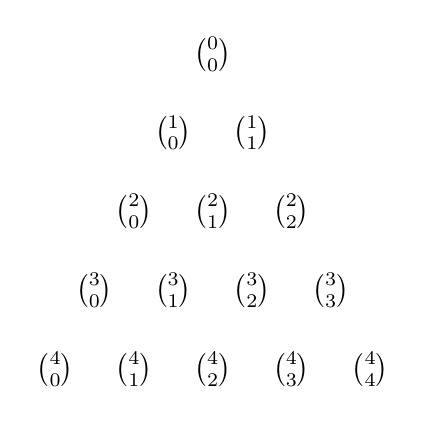
\begin{tikzpicture}
\foreach \n in {0,...,4} {
  \foreach \k in {0,...,\n} {
    \node at (\k-\n/2,-\n) {${\n \choose \k}$};
  }
}
\end{tikzpicture}

Notice, the sum of the nth row seems to be $2^n$.


\subsection{Sidenote 1: Left Boundary}\label{pas:pascal_sidenote1}
Prove that $${p \choose 0}={p+1 \choose 0}$$
Proof:
$${p \choose 0}=\frac{p!}{0! \cdot (p-0)!}=\frac{p!}{p!}=1=\frac{(p+1)!}{0! \cdot (p+1-0)!}={p+1 \choose 0}$$

\subsection{Sidenote 2: Right Boundary}\label{pas:pascal_sidenote2}
Prove that $${p \choose p}={p+1 \choose p+1}$$

Proof:
$${p \choose p}=\frac{p!}{0! \cdot (p-0)!}=\frac{p!}{p!}=1=\frac{(p+1)!}{0! \cdot (p+1-0)!}={p+1 \choose p+1}$$

\subsection{Sidenote 3: Pascal's Recurrence}\label{pas:pascal_sidenote3}
Prove that $${p \choose q} +{p \choose q+1}={p+1 \choose q+1}$$

Proof:
$${p \choose q} +{p \choose q+1}=\frac{p!}{q! \cdot (p-q)!}+\frac{p!}{(q+1)! \cdot (p-q-1)!} $$
$$=\frac{p! \cdot (q+1)}{(q+1)! \cdot (p-q)!}+\frac{p! \cdot (p-q)}{(q+1)! \cdot (p-q)!} $$
$$= \frac{p! \cdot (q+1+p-q)}{(q+1)! \cdot (p-q)!} = \frac{p! \cdot (p+1)}{(q+1)! \cdot (p-q)!}$$
$$=\frac{(p+1)!}{(q+1)! \cdot (p-q)!}={p+1 \choose q+1} $$


\subsection{Proof by Induction}\label{pas:proof_by_induction} 

for n=0:
$${0 \choose 0} = \frac{0!}{0! \cdot 0!}=1=2^0$$

Assume n=k works:
$${k \choose 0} + {k \choose 1} +
{k \choose 2}+...+{k \choose k-2}+{k \choose k-1}+{k \choose k} =2^k$$
Prove for n=k+1
$${k+1 \choose 0} + {k+1 \choose 1} +
{k+1 \choose 2}+...+{k+1 \choose k-1}+{k+1 \choose k}+{k+1 \choose k+1}$$

Using sidenote 1, replace ${k+1 \choose 0}$ with ${k \choose 0}$\\

Using sidenote 2, replace ${k+1 \choose k+1}$ with ${k \choose k}$\\

Using sidenote 2, replace ${k+1 \choose q+1}$ with ${k \choose q} +{k \choose q+1}$\\

$$={k \choose 0} + {k \choose 0}+ {k \choose 1} + {k \choose 1}+ {k \choose 2}+...+{k \choose k-2}+{k \choose k-1}+{k \choose k-1}+{k \choose k}+{k \choose k}$$
$$=2 \cdot ({k \choose 0} + {k \choose 1} +
{k \choose 2}+...+{k \choose k-2}+{k \choose k-1}+{k \choose k}) =2 \cdot (2^k)= 2^{k+1}$$

Therefore, proven by induction.

\end{document}

\clearpage

\documentclass[a4paper]{article}

% Shared Preamble for MathLatexDocs

% --- Core Packages ---
\usepackage[english]{babel}
\usepackage[utf8]{inputenc}
\usepackage{amsmath}
\usepackage{amsthm}
\usepackage{amssymb}
\usepackage{mathtools}
\usepackage{graphicx}
\usepackage{microtype} % Better justification and fewer overfull hboxes
\usepackage{bm}
\usepackage{enumitem}
\usepackage{booktabs}
\usepackage{mathrsfs}

% --- Layout & Design ---
\usepackage{docmute}
\usepackage{subfiles} % Support for master/subfile structure
\usepackage[colorinlistoftodos]{todonotes}
\usepackage[colorlinks=true, linkcolor=blue, citecolor=magenta]{hyperref}
\usepackage{cleveref} % Better cross-referencing
\usepackage{tcolorbox} % For styled boxes
\usepackage{tikz} % For drawing diagrams
\usetikzlibrary{arrows.meta,positioning}

% --- Theorem Environments (Classic Style) ---
\makeatletter
\@ifundefined{classicthm}{%
  \newtheorem{classicthm}{Theorem}[section]
  \newtheorem{classicdef}[classicthm]{Definition}
  \newtheorem{classiclem}[classicthm]{Lemma}
  \newtheorem{theorem}{Theorem}[section]
  \newtheorem{corollary}{Corollary}[theorem]
  \newtheorem{lemma}[theorem]{Lemma}
  \newtheorem{definition}{Definition}[section]
  \newtheorem{proposition}[theorem]{Proposition}
  \newtheorem{remark}[theorem]{Remark}
  \newtheorem{example}[theorem]{Example}
}{}

% Wrappers to maintain compatibility with the {Title}{Label} syntax used in files
\@ifundefined{mytheorem}{%
  \newenvironment{mytheorem}[2]{%
    \begin{classicthm}[#1]\label{thm:#2}
  }{%
    \end{classicthm}
  }
  
  \newenvironment{mydefinition}[2]{%
    \begin{classicdef}[#1]\label{def:#2}
  }{%
    \end{classicdef}
  }
  
  \newenvironment{mylemma}[2]{%
    \begin{classiclem}[#1]\label{lem:#2}
  }{%
    \end{classiclem}
  }
}{}
\makeatother

% --- Custom Commands ---
\providecommand{\Z}{\mathbb{Z}}
\providecommand{\R}{\mathbb{R}}
\providecommand{\C}{\mathbb{C}}
\providecommand{\N}{\mathbb{N}}
\providecommand{\G}{\mathcal{G}}
\providecommand{\Lop}{\mathcal{L}}
\providecommand{\PP}{\mathcal{P}}
\providecommand{\dd}{\,\mathrm{d}}
\providecommand{\bitand}{\mathbin{\&}}
\providecommand{\CFDots}{\genfrac{}{}{0pt}{0}{}{\ddots}}


\title{Geometric Series}
\author{Emil Kerimov}
\date{\today}

\begin{document}
\maketitle
\section{Geometric Series}\label{gs:Geometric Series}

Prove that:

$$\sum\limits_{i=1}^{n} a\cdot r^{i-1} =  \frac{a\cdot(1-r^{n+1})}{1-r}$$

Proof:

Define $S_n$ such that:

$$S_{n} = a + ar + ar^2 + ... + ar^{n-1}+ar^n$$
Note that $$r\cdot S_{n} = ar + ar^2 + ... + ar^{n-1} + ar^n + ar^{n+1}$$
Such that $$S_{n}-r\cdot S_{n} = a-ar^{n+1}$$
$$=>
S_{n} = \frac{a\cdot(1-r^{n+1})}{1-r}
$$


If $|r|<1$:

Then 
$$\sum\limits_{i=1}^{\infty} a\cdot r^{i-1}
= \lim_{n \to +\infty}\frac{a\cdot(1-r^{n+1})}{1-r}
= \frac{a}{1-r}
$$

Note that by taking derivatives of both sides and a bit of reindexing:

$$\sum\limits_{i=0}^{\infty} \frac{d}{dr}a\cdot r^{i}
=\sum\limits_{i=0}^{\infty} i\cdot a\cdot r^{i-1}
=0+\sum\limits_{i=1}^{\infty} i\cdot a\cdot r^{i-1}
= \frac{a}{(1-r)^2}
$$

$$=>
\sum\limits_{i=1}^{\infty} i\cdot r^{i}
= \frac{r}{(1-r)^2} \mbox{ when } |r|<1
$$
\end{document}

\clearpage

\documentclass[a4paper]{article}

% Shared Preamble for MathLatexDocs

% --- Core Packages ---
\usepackage[english]{babel}
\usepackage[utf8]{inputenc}
\usepackage{amsmath}
\usepackage{amsthm}
\usepackage{amssymb}
\usepackage{mathtools}
\usepackage{graphicx}
\usepackage{microtype} % Better justification and fewer overfull hboxes
\usepackage{bm}
\usepackage{enumitem}
\usepackage{booktabs}
\usepackage{mathrsfs}

% --- Layout & Design ---
\usepackage{docmute}
\usepackage{subfiles} % Support for master/subfile structure
\usepackage[colorinlistoftodos]{todonotes}
\usepackage[colorlinks=true, linkcolor=blue, citecolor=magenta]{hyperref}
\usepackage{cleveref} % Better cross-referencing
\usepackage{tcolorbox} % For styled boxes
\usepackage{tikz} % For drawing diagrams
\usetikzlibrary{arrows.meta,positioning}

% --- Theorem Environments (Classic Style) ---
\makeatletter
\@ifundefined{classicthm}{%
  \newtheorem{classicthm}{Theorem}[section]
  \newtheorem{classicdef}[classicthm]{Definition}
  \newtheorem{classiclem}[classicthm]{Lemma}
  \newtheorem{theorem}{Theorem}[section]
  \newtheorem{corollary}{Corollary}[theorem]
  \newtheorem{lemma}[theorem]{Lemma}
  \newtheorem{definition}{Definition}[section]
  \newtheorem{proposition}[theorem]{Proposition}
  \newtheorem{remark}[theorem]{Remark}
  \newtheorem{example}[theorem]{Example}
}{}

% Wrappers to maintain compatibility with the {Title}{Label} syntax used in files
\@ifundefined{mytheorem}{%
  \newenvironment{mytheorem}[2]{%
    \begin{classicthm}[#1]\label{thm:#2}
  }{%
    \end{classicthm}
  }
  
  \newenvironment{mydefinition}[2]{%
    \begin{classicdef}[#1]\label{def:#2}
  }{%
    \end{classicdef}
  }
  
  \newenvironment{mylemma}[2]{%
    \begin{classiclem}[#1]\label{lem:#2}
  }{%
    \end{classiclem}
  }
}{}
\makeatother

% --- Custom Commands ---
\providecommand{\Z}{\mathbb{Z}}
\providecommand{\R}{\mathbb{R}}
\providecommand{\C}{\mathbb{C}}
\providecommand{\N}{\mathbb{N}}
\providecommand{\G}{\mathcal{G}}
\providecommand{\Lop}{\mathcal{L}}
\providecommand{\PP}{\mathcal{P}}
\providecommand{\dd}{\,\mathrm{d}}
\providecommand{\bitand}{\mathbin{\&}}
\providecommand{\CFDots}{\genfrac{}{}{0pt}{0}{}{\ddots}}


\title{Sequences}
\author{Emil Kerimov}
\date{\today}
\begin{document}
\maketitle


\section{Arithmetic Sequence}\label{sas:sec:arithmetic-sequence}

\begin{definition}\label{sas:Arithmetic def}
Given a starting value of $a_0$ and a constant difference value of $d$ the arithmetic sequence is defined as follows.
\[\boxed{
a_n = a_0 + n \cdot d
}
\]
\end{definition}

\subsection{Sum of Arithmetic sequence}\label{sas:subsec:sum-of-arithmetic-sequence}


\begin{theorem}
\begin{equation} \label{sas:eq:sum-of-arithmetic-sequence}
\sum\limits_{k=0}^{n} a_k = \frac{(n+1)}{2} ( 2 a_0 +n \cdot d )
\end{equation}

Proof
\begin{gather*}
\intertext{Define $S_n$ such that:}
S_{n} = \sum_{k=0}^{n} a_k 
\\
\intertext{Note that}
2 S_{n} = \sum_{k=0}^{n} a_k + \sum_{k=0}^{n} a_{n-k} = \sum_{k=0}^{n} \Big( a_k + a_{n-k} \Big)
\\
\intertext{Using the definition we see $a_k + a_{n-k} = \big( a_0 + k \cdot d \big) + \big( a_0 + (n-k) \cdot d \big) =  2 a_0 +n \cdot d $ which does not depend on $k$}
\\
2 S_{n} = \sum_{k=0}^{n} \Big( 2 a_0 +n \cdot d \Big) = (n+1) \Big( 2 a_0 +n \cdot d \Big)
\\
S_{n} = \frac{(n+1)}{2} ( 2 a_0 +n \cdot d )
\end{gather*}
\end{theorem}

\subsection{Example: Sum of Natural Numbers}\label{sas:Sum of Natural Numbers}
Prove that $$\sum\limits_{i=0}^{n} i = 0+ 1+2+3+...+n = \frac{n(n+1)}{2}$$

Proof:
Set $a_0 = 0$ and $d=1$
$$\sum\limits_{i=0}^{n} i
=
\frac{(n+1)}{2} (n )$$

\end{document}

\clearpage

\documentclass[a4paper]{article}

% Shared Preamble for MathLatexDocs

% --- Core Packages ---
\usepackage[english]{babel}
\usepackage[utf8]{inputenc}
\usepackage{amsmath}
\usepackage{amsthm}
\usepackage{amssymb}
\usepackage{mathtools}
\usepackage{graphicx}
\usepackage{microtype} % Better justification and fewer overfull hboxes
\usepackage{bm}
\usepackage{enumitem}
\usepackage{booktabs}
\usepackage{mathrsfs}

% --- Layout & Design ---
\usepackage{docmute}
\usepackage{subfiles} % Support for master/subfile structure
\usepackage[colorinlistoftodos]{todonotes}
\usepackage[colorlinks=true, linkcolor=blue, citecolor=magenta]{hyperref}
\usepackage{cleveref} % Better cross-referencing
\usepackage{tcolorbox} % For styled boxes
\usepackage{tikz} % For drawing diagrams
\usetikzlibrary{arrows.meta,positioning}

% --- Theorem Environments (Classic Style) ---
\makeatletter
\@ifundefined{classicthm}{%
  \newtheorem{classicthm}{Theorem}[section]
  \newtheorem{classicdef}[classicthm]{Definition}
  \newtheorem{classiclem}[classicthm]{Lemma}
  \newtheorem{theorem}{Theorem}[section]
  \newtheorem{corollary}{Corollary}[theorem]
  \newtheorem{lemma}[theorem]{Lemma}
  \newtheorem{definition}{Definition}[section]
  \newtheorem{proposition}[theorem]{Proposition}
  \newtheorem{remark}[theorem]{Remark}
  \newtheorem{example}[theorem]{Example}
}{}

% Wrappers to maintain compatibility with the {Title}{Label} syntax used in files
\@ifundefined{mytheorem}{%
  \newenvironment{mytheorem}[2]{%
    \begin{classicthm}[#1]\label{thm:#2}
  }{%
    \end{classicthm}
  }
  
  \newenvironment{mydefinition}[2]{%
    \begin{classicdef}[#1]\label{def:#2}
  }{%
    \end{classicdef}
  }
  
  \newenvironment{mylemma}[2]{%
    \begin{classiclem}[#1]\label{lem:#2}
  }{%
    \end{classiclem}
  }
}{}
\makeatother

% --- Custom Commands ---
\providecommand{\Z}{\mathbb{Z}}
\providecommand{\R}{\mathbb{R}}
\providecommand{\C}{\mathbb{C}}
\providecommand{\N}{\mathbb{N}}
\providecommand{\G}{\mathcal{G}}
\providecommand{\Lop}{\mathcal{L}}
\providecommand{\PP}{\mathcal{P}}
\providecommand{\dd}{\,\mathrm{d}}
\providecommand{\bitand}{\mathbin{\&}}
\providecommand{\CFDots}{\genfrac{}{}{0pt}{0}{}{\ddots}}


\title{Recursive Sum of Powers}
\author{Emil Kerimov}
\date{\today}
\begin{document}
\maketitle

\section{Recursive Sum of Powers}
\label{rsp:Recursive sum of powers}

To solve for $\sum\limits_{i=1}^{n} i^{p}$ consider $\sum\limits_{i=1}^{n} {(1+i)^{p+1} - i^{p+1}} = (1+n)^{p+1} - 1$

\subsection{Sum of Squares}

Let p=2

$$\sum\limits_{i=1}^{n} (1+i)^3 - i^3 = \sum\limits_{i=1}^{n} 1+3i+3i^2 +i^3 - i^3 = \sum\limits_{i=1}^{n} 1+3i+3i^2$$

and 

$$\sum\limits_{i=1}^{n} (1+i)^3 - i^3 = (n+1)^3 - 1$$

Hence

$$\sum\limits_{i=1}^{n} 1+ 3\sum\limits_{i=1}^{n}i+3\sum\limits_{i=1}^{n}i^2 =(n+1)^3 - 1$$

$$n+3\frac{n(n-1)}{2}+3\sum\limits_{i=1}^{n}i^2 =(n+1)^3 - 1$$


$$3\sum\limits_{i=1}^{n}i^2 = n^3 + 3n^2 + 3n + 1 - n - 3\frac{n(n-1)}{2}$$


$$3\sum\limits_{i=1}^{n}i^2 = n(n+1)(n+\frac{1}{2})$$


$$
\boxed{
\sum\limits_{i=1}^{n}i^2 = \frac{n}{3} \cdot (n+1) \cdot (n+\frac{1}{2})
}
$$

\subsection{Sum of Cubes}

Let p=3

$$\sum\limits_{i=1}^{n} (1+i)^4 - i^4 = \sum\limits_{i=1}^{n} 1+4i+6i^2 + 4i^3 +i^4 - i^4 = \sum\limits_{i=1}^{n} 1+4i+6i^2 + 4i^3$$

and 

$$\sum\limits_{i=1}^{n} (1+i)^4 - i^4 = (n+1)^4 - 1$$

Hence

$$\sum\limits_{i=1}^{n} 1+ 4\sum\limits_{i=1}^{n}i + 6\sum\limits_{i=1}^{n}i^2
+ 4\sum\limits_{i=1}^{n}i^3 =(n+1)^4 - 1$$

$$n+4\frac{n(n-1)}{2}+6 \frac{n}{3} \cdot (n+1) \cdot (n+\frac{1}{2}) + 4\sum\limits_{i=1}^{n}i^3 =(n+1)^4 - 1$$


$$4\sum\limits_{i=1}^{n}i^3 = n^4 + 4n^3 + 6n^2 + 4n - n - 2n(n-1) - n\cdot (n+1) \cdot (2n+1)$$

Simplifying

$$4\sum\limits_{i=1}^{n}i^3 = n^4 + 2n^3 + n^2 $$

$$4\sum\limits_{i=1}^{n}i^3 = n^2 (n^2 + 2n + 1) = n^2(n+1)^2$$

$$
\boxed{
\sum\limits_{i=1}^{n}i^3 = \Big( \frac{n(n+1)}{2} \Big)^2
}
$$

\end{document}

\clearpage

% ========================================================
\part{Algebra \& Polynomials}
% ========================================================
\documentclass[a4paper]{article}

% Shared Preamble for MathLatexDocs

% --- Core Packages ---
\usepackage[english]{babel}
\usepackage[utf8]{inputenc}
\usepackage{amsmath}
\usepackage{amsthm}
\usepackage{amssymb}
\usepackage{mathtools}
\usepackage{graphicx}
\usepackage{microtype} % Better justification and fewer overfull hboxes
\usepackage{bm}
\usepackage{enumitem}
\usepackage{booktabs}
\usepackage{mathrsfs}

% --- Layout & Design ---
\usepackage{docmute}
\usepackage{subfiles} % Support for master/subfile structure
\usepackage[colorinlistoftodos]{todonotes}
\usepackage[colorlinks=true, linkcolor=blue, citecolor=magenta]{hyperref}
\usepackage{cleveref} % Better cross-referencing
\usepackage{tcolorbox} % For styled boxes
\usepackage{tikz} % For drawing diagrams
\usetikzlibrary{arrows.meta,positioning}

% --- Theorem Environments (Classic Style) ---
\makeatletter
\@ifundefined{classicthm}{%
  \newtheorem{classicthm}{Theorem}[section]
  \newtheorem{classicdef}[classicthm]{Definition}
  \newtheorem{classiclem}[classicthm]{Lemma}
  \newtheorem{theorem}{Theorem}[section]
  \newtheorem{corollary}{Corollary}[theorem]
  \newtheorem{lemma}[theorem]{Lemma}
  \newtheorem{definition}{Definition}[section]
  \newtheorem{proposition}[theorem]{Proposition}
  \newtheorem{remark}[theorem]{Remark}
  \newtheorem{example}[theorem]{Example}
}{}

% Wrappers to maintain compatibility with the {Title}{Label} syntax used in files
\@ifundefined{mytheorem}{%
  \newenvironment{mytheorem}[2]{%
    \begin{classicthm}[#1]\label{thm:#2}
  }{%
    \end{classicthm}
  }
  
  \newenvironment{mydefinition}[2]{%
    \begin{classicdef}[#1]\label{def:#2}
  }{%
    \end{classicdef}
  }
  
  \newenvironment{mylemma}[2]{%
    \begin{classiclem}[#1]\label{lem:#2}
  }{%
    \end{classiclem}
  }
}{}
\makeatother

% --- Custom Commands ---
\providecommand{\Z}{\mathbb{Z}}
\providecommand{\R}{\mathbb{R}}
\providecommand{\C}{\mathbb{C}}
\providecommand{\N}{\mathbb{N}}
\providecommand{\G}{\mathcal{G}}
\providecommand{\Lop}{\mathcal{L}}
\providecommand{\PP}{\mathcal{P}}
\providecommand{\dd}{\,\mathrm{d}}
\providecommand{\bitand}{\mathbin{\&}}
\providecommand{\CFDots}{\genfrac{}{}{0pt}{0}{}{\ddots}}


\title{Deriving the Quadratic equation}
\author{Emil Kerimov}
\date{\today}
\begin{document}
\maketitle

\section{The Quadratic Equation}

Given a quadratic polynomial $ax^2 + bx + c = 0$
The two solutions of $x$ that satisfy this equation are given by the quadratic equation
\begin{equation}
x = \frac{-b \pm \sqrt{b^2 - 4ac}}{2a}
\end{equation}

\section{Algebraic Proof via Completing the Square}
The most straight-forward proof is given by a technique referred to as 'Completing the Square'.

\begin{gather*}
ax^2 + bx + c = 0\\
\shortintertext{Dividing both sides by $a$}
x^2 + \frac{b}{a}x + \frac{c}{a} = 0\\
\shortintertext{Adding and subtracting $\frac{b^2}{(2a)^2}$}
x^2 + \frac{b}{a}x + \frac{b^2}{(2a)^2} +  \frac{c}{a} - \frac{b^2}{(2a)^2} = 0\\
\shortintertext{Recognizing the 'square'}
(x+ \frac{b}{2a})^2 +  \frac{c}{a} - \frac{b^2}{(2a)^2} = 0\\
\shortintertext{Rearranging and solving}
\begin{alignedat}{2}
(x + \frac{b}{2a})^2 &= \frac{b^2}{4a^2}-  \frac{c}{a}  = \frac{b^2-4ac}{4a^2}\\
x + \frac{b}{2a} &=\pm \sqrt{ \frac{b^2 - 4ac}{4a^2}}\\
x  &= - \frac{b}{2a} \pm \sqrt{ \frac{b^2 - 4ac}{4a^2}}\\
x  &= \frac{-b \pm \sqrt{b^2 - 4ac}}{2a}\\
\end{alignedat}
\end{gather*}


\end{document}

\clearpage

\documentclass[a4paper]{article}

% Shared Preamble for MathLatexDocs

% --- Core Packages ---
\usepackage[english]{babel}
\usepackage[utf8]{inputenc}
\usepackage{amsmath}
\usepackage{amsthm}
\usepackage{amssymb}
\usepackage{mathtools}
\usepackage{graphicx}
\usepackage{microtype} % Better justification and fewer overfull hboxes
\usepackage{bm}
\usepackage{enumitem}
\usepackage{booktabs}
\usepackage{mathrsfs}

% --- Layout & Design ---
\usepackage{docmute}
\usepackage{subfiles} % Support for master/subfile structure
\usepackage[colorinlistoftodos]{todonotes}
\usepackage[colorlinks=true, linkcolor=blue, citecolor=magenta]{hyperref}
\usepackage{cleveref} % Better cross-referencing
\usepackage{tcolorbox} % For styled boxes
\usepackage{tikz} % For drawing diagrams
\usetikzlibrary{arrows.meta,positioning}

% --- Theorem Environments (Classic Style) ---
\makeatletter
\@ifundefined{classicthm}{%
  \newtheorem{classicthm}{Theorem}[section]
  \newtheorem{classicdef}[classicthm]{Definition}
  \newtheorem{classiclem}[classicthm]{Lemma}
  \newtheorem{theorem}{Theorem}[section]
  \newtheorem{corollary}{Corollary}[theorem]
  \newtheorem{lemma}[theorem]{Lemma}
  \newtheorem{definition}{Definition}[section]
  \newtheorem{proposition}[theorem]{Proposition}
  \newtheorem{remark}[theorem]{Remark}
  \newtheorem{example}[theorem]{Example}
}{}

% Wrappers to maintain compatibility with the {Title}{Label} syntax used in files
\@ifundefined{mytheorem}{%
  \newenvironment{mytheorem}[2]{%
    \begin{classicthm}[#1]\label{thm:#2}
  }{%
    \end{classicthm}
  }
  
  \newenvironment{mydefinition}[2]{%
    \begin{classicdef}[#1]\label{def:#2}
  }{%
    \end{classicdef}
  }
  
  \newenvironment{mylemma}[2]{%
    \begin{classiclem}[#1]\label{lem:#2}
  }{%
    \end{classiclem}
  }
}{}
\makeatother

% --- Custom Commands ---
\providecommand{\Z}{\mathbb{Z}}
\providecommand{\R}{\mathbb{R}}
\providecommand{\C}{\mathbb{C}}
\providecommand{\N}{\mathbb{N}}
\providecommand{\G}{\mathcal{G}}
\providecommand{\Lop}{\mathcal{L}}
\providecommand{\PP}{\mathcal{P}}
\providecommand{\dd}{\,\mathrm{d}}
\providecommand{\bitand}{\mathbin{\&}}
\providecommand{\CFDots}{\genfrac{}{}{0pt}{0}{}{\ddots}}


\title{Exact solution to Polynomial equations}
\author{Emil Kerimov}
\date{}


\begin{document}
\maketitle

\section{Historical Background of Polynomial Solutions}\label{eps:sec:history}

Scipione del Ferro is thought to have been the first to discover the general solution to the cubic equation, but did not publish it, and kept it a secret until his deathbed, telling his student Antonio Fior.
Fior then challenged Niccolo Fontana, also known as Tartaglia, in 1535 to solve a list of 30 depressed cubics.
On the night of February 13, 1535, Tartaglia discovered the solution.

\bigskip

Tartaglia revealed the secret to
Gerolamo Cardano on March 25, 1539, with the oath
of Cardano to never publish the findings.
Cardano, along with his pupil Ludovico Ferrari, discovered the solution of the general cubic equation.

While inspecting del Ferro's papers, they
came across a solution to the depressed cubic in del Ferro's own handwriting.
Cardano and Ferrari were no longer prohibited from publishing their results.

\bigskip

In 1545, Cardano published his book Ars
Magna, the \textquotedblleft Great Art.\textquotedblright
In it, he published the solution to the
depressed cubic, with a preface crediting
del Ferro with the original solution.
He also published his solution of the
general cubic and also Ferrari's solution of
the quartic.

\bigskip

Lagrange published a paper in 1771, Reflections on the Algebraic Theory of Equations, in which he described why the techniques used to solve the quadratic, cubic and quartic equations could not be applied to solve the quintic equation.

\bigskip

Paolo Ruffini attempted to prove that the quintic equation was insolvable.
He published 6 proofs on the subject from 1799 to 1813.
However, other mathematicians found his work too long and difficult to understand, except for Cauchy.
These proofs did end up having a few gaps in them, but were on the right track.

\bigskip

Niels Henrik Abel published his proof that the quintic equation was insolvable in 1824.
Abel is credited for finally putting this question to rest.

\bigskip

Evariste Galois, who died at the age of 20 in 1832 in a duel, studied attempted to generalize how to determine when the roots could be solved in terms of radicals.
He became the first mathematician to use the word 'group' and defined the normal subgroup.

\section{Quadratic}\label{eps:sec:quadratic}

\begin{definition}\label{eps:quad def}
  A quadratic polynomial
  \[
    ax^2 + bx + c = 0
  \]
\end{definition}

Given a quadratic polynomial, the two solutions of $x$ that satisfy this equation are given by the quadratic equation
\begin{equation}
  \boxed{
    x = \frac{-b \pm \sqrt{b^2 - 4ac}}{2a}
  }\label{eps:eq:equation}
\end{equation}

This one equation has three solutions due to the cube root of complex numbers.

\subsection{Algebraic Proof}\label{eps:subsec:algebraic-proof}
The most straight-forward proof is given by a technique referred to as 'Completing the Square'.

\begin{gather*}
  ax^2 + bx + c = 0\\
  \shortintertext{Dividing both sides by $a$}
  x^2 + \frac{b}{a}x + \frac{c}{a} = 0\\
  \shortintertext{Adding and subtracting $\frac{b^2}{(2a)^2}$}
  x^2 + \frac{b}{a}x + \frac{b^2}{(2a)^2} +  \frac{c}{a} - \frac{b^2}{(2a)^2} = 0\\
  \shortintertext{Recognizing the 'square'}
  (x+ \frac{b}{2a})^2 +  \frac{c}{a} - \frac{b^2}{(2a)^2} = 0\\
  \shortintertext{Rearranging and solving}
  \begin{alignedat}{2}
    (x + \frac{b}{2a})^2 & = \frac{b^2}{4a^2}-  \frac{c}{a}  = \frac{b^2-4ac}{4a^2} \\
    x + \frac{b}{2a}     & =\pm \sqrt{ \frac{b^2 - 4ac}{4a^2}}                      \\
    x                    & = - \frac{b}{2a} \pm \sqrt{ \frac{b^2 - 4ac}{4a^2}}      \\
    x                    & = \frac{-b \pm \sqrt{b^2 - 4ac}}{2a}                     \\
  \end{alignedat}
\end{gather*}

\subsection{Discriminant}\label{eps:subsec:discriminant}

The discriminant of a quadratic equation is defined to be
\begin{equation}
  \Delta = b^2 - 4ac\label{eps:eq:equation2}
\end{equation}

\section{Cubic}\label{eps:sec:cubic}

\begin{definition}\label{eps:cubic def}
  A cubic polynomial
  \[
    ax^3 + bx^2 + cx + d = 0
  \]
\end{definition}

Given a cubic polynomial the three solutions of $x$ that satisfy this equation are given by

\begin{equation} \label{eps:eq:cubic-solution}
  \boxed{
    \begin{split}
      x = - \frac{b}{3a} +
      \frac{1}{\sqrt[3]{2} \cdot 3 a} \Bigg(
      \sqrt[3]{9abc - 27 d a^2 - 2 b^3  + 3a \sqrt[2]{
          3 \Big(
          27 a^2 d^2 + 4 b^3 d - 18 abcd + 4 a c^3 - b^2 c^2
          \Big)
        }}
      \\
      +
      \sqrt[3]{9abc - 27 d a^2 - 2 b^3 -
        3a \sqrt[2]{
          3
          \Big(
          27 a^2 d^2 + 4 b^3 d - 18 abcd + 4 a c^3 - b^2 c^2
          \Big)
        }}
      \Bigg)
    \end{split}
  }
\end{equation}

This was first shown by Gerolamo Cardano in 1545

\subsection{Depressed Cubic}\label{eps:subsec:depressed-cubic}
\begin{definition}\label{eps:depressed cubic def}
  A depressed cubic is a polynomial in the form of
  \[
    x^3 + cx + d = 0
  \]
\end{definition}


\begin{theorem}
  We can transform any cubic to a depressed cubic form.

  Proof
  \begin{gather*}
    \intertext{Starting from definition~\ref{eps:cubic def}}
    ax^3 + bx^2 + cx + d = 0
    \\
    \intertext{Dividing by a, we define}
    a_2 = \frac{b}{a}, a_1 = \frac{c}{a}, a_0 = \frac{d}{a}
    \\
    \intertext{Rewriting}
    x^3 + a_2 x^2 + a_1 x + a_0 = 0
    \\
    \intertext{Completing the cube}
    x^3 + 3 \Big( \frac{a_2}{3} \Big) x^2 + 3 \Big( \frac{a_2}{3} \Big)^2 x  + \Big( \frac{a_2}{3} \Big)^3 - 3 \Big( \frac{a_2}{3} \Big)^2 x  - \Big( \frac{a_2}{3} \Big)^3 + a_1 x + a_0 = 0
    \\
    \intertext{Using $(x+t)^3 = x^3 + 3x^2 t + 3x t^2 + t^3$}
    \Big( x + \frac{a_2}{3} \Big)^3 + x \Big( a_1 - 3 \Big( \frac{a_2}{3} \Big)^2 \Big)  + \Big( a_0 - \Big( \frac{a_2}{3} \Big)^3 \Big) = 0
    \\
    \intertext{Let $z=x + \frac{a_2}{3}$}
    z^3 + \Big(z - \frac{a_2}{3} \Big) \Big( a_1 - 3 \Big( \frac{a_2}{3} \Big)^2 \Big)  + \Big( a_0 - \Big( \frac{a_2}{3} \Big)^3 \Big) = 0
    \\
    \intertext{Simplifying and collecting like terms}
    z^3 +
    z \Big( a_1 - 3 \Big( \frac{a_2}{3} \Big)^2 \Big)
    +\Bigg(
    - \frac{a_2}{3} \Big( a_1 - 3 \Big( \frac{a_2}{3} \Big)^2 \Big)
    + \Big( a_0 - \Big( \frac{a_2}{3} \Big)^3 \Big)
    \Bigg) = 0
    \\
    \intertext{Therefore after shifting with $z=x + \frac{b}{3a}$}
    c' = \frac{c}{a} - 3 \Big( \frac{b}{3a} \Big)^2
    \\
    d' = - \frac{b}{3a} \Big( \frac{c}{a} - 3 \Big( \frac{b}{3a} \Big)^2 \Big)
    + \Big( \frac{d}{a} - \Big( \frac{b}{3a} \Big)^3 \Big)
    \intertext{Simplifying}
    c' =  \frac{c}{a} - 3 \Big( \frac{b}{3a} \Big)^2
    \\
    d' =\frac{d}{a} - \Big( \frac{b}{3a} \Big)^3 - \frac{b}{3a} c'
  \end{gather*}
\end{theorem}


\begin{theorem}
  Starting from the depressed cubic form, we can solve for the roots.

  Proof
  \begin{gather*}
    \intertext{Starting from definition~\ref{eps:depressed cubic def}}
    z^3 + cz + d = 0
    \\
    \intertext{Define $p=-\frac{c}{3}$ and $q=-\frac{d}{2} $}
    z^3 = 3pz + 2q
    \\
    \intertext{Consider $z=u+v$}
    z^3 = (u+v)^3 = u^3 + 3u^2 v + 3 u v^2 + v^3 = u^3 + v^3 + 3uv(u+v) = 3uv(z) + u^3 + v^3
    \\
    \intertext{Comparing these forms}
    3uv = 3p \\
    u^3 + v^3 = 2q \\
    \intertext{This implies}
    v = \frac{p}{u}\\
    u^3 + \Big(\frac{p}{u}\Big)^3 = 2q
    \intertext{Therefore we can create a polynomial equation to solve for this relation}
    u^6 + -2q u^3 + p^3 = 0
    \\
    \intertext{We can use the quadratic solution to solve for this relation}
    u^3 = \frac{2q \pm \sqrt{4q^2 - 4p^3}}{2} = q \pm \sqrt{q^2 - p^3}
    \\
    \intertext{Define the solutions for u}
    u_{+} = \sqrt[3]{q + \sqrt{q^2 - p^3}} \\
    u_{-} = \sqrt[3]{q - \sqrt{q^2 - p^3}} \\
    \intertext{Since $u_{+}^3 u_{-}^3  = p^3$, from quadratic equation}
    u_{+}u_{-} = p
    \intertext{Using definition $v = \frac{p}{u}$}
    v_{+} = \frac{p}{u_{+}} =\frac{p u_{-}}{u_{+}u_{-}} = \frac{p u_{-}}{p} =  u_{-}
    \intertext{Similarly}
    v_{-} =  u_{+}
    \intertext{Therefore the solution to $z^3 = 3pz + 2q$}
    z = u + v = u_{+} + u_{-} =  \sqrt[3]{q + \sqrt{q^2 - p^3}} + \sqrt[3]{q - \sqrt{q^2 - p^3}}
    \intertext{Re-writing in the original form}
    z = \sqrt[3]{-\frac{d}{2} + \sqrt{\frac{d^2}{4} +\frac{c^3}{27}}} + \sqrt[3]{-\frac{d}{2} - \sqrt{\frac{d^2}{4} + \frac{c^3}{27}}}
  \end{gather*}
\end{theorem}



\subsection{General Cubic}\label{eps:subsec:general-cubic}
Combining all of these results to back out the solution for a general cubic equation in terms of the original variables, $ax^3 + bx^2 + cx + d = 0$,
we first summarize the steps taken.

\begin{itemize}
  \item shift solution by $z=x + \frac{b}{3a}$
  \item write solution in depressed cubic form
  \item solve the depressed cubic equation.
\end{itemize}

Undoing these substitutions backwards
\begin{gather*}
  z = \sqrt[3]{-\frac{d'}{2} + \sqrt[2]{\frac{d'^2}{4} +\frac{c'^3}{27}}} + \sqrt[3]{-\frac{d'}{2} - \sqrt[2]{\frac{d'^2}{4} + \frac{c'^3}{27}}}
  \\
  \intertext{Using $ c' =  \frac{c}{a} - 3 \Big( \frac{b}{3a} \Big)^2 $
    and
    $d' =\frac{d}{a} - \Big( \frac{b}{3a} \Big)^3 - \frac{b}{3a} c' $}
  z = \sqrt[3]{-\frac{\Big( \frac{d}{a} - \Big( \frac{b}{3a} \Big)^3 - \frac{b}{3a} \Big( \frac{c}{a} - 3 \Big( \frac{b}{3a} \Big)^2 \Big)}{2} + \sqrt[2]{\frac{\Big(\frac{d}{a} - \Big( \frac{b}{3a} \Big)^3 - \frac{b}{3a} \Big( \frac{c}{a} - 3 \Big( \frac{b}{3a} \Big)^2 \Big)^2}{4} +\frac{\Big( \frac{c}{a} - 3 \Big( \frac{b}{3a} \Big)^2 \Big)^3}{27}}}
  \\
  +
  \sqrt[3]{-\frac{\Big( \frac{d}{a} - \Big( \frac{b}{3a} \Big)^3 - \frac{b}{3a} \Big( \frac{c}{a} - 3 \Big( \frac{b}{3a} \Big)^2 \Big)}{2} - \sqrt[2]{\frac{\Big(\frac{d}{a} - \Big( \frac{b}{3a} \Big)^3 - \frac{b}{3a} \Big( \frac{c}{a} - 3 \Big( \frac{b}{3a} \Big)^2 \Big)^2}{4} +\frac{\Big( \frac{c}{a} - 3 \Big( \frac{b}{3a} \Big)^2 \Big)^3}{27}}}
  \\
  \intertext{Simplifying}
  c' = \frac{c}{a} - 3 \Big( \frac{b}{3a} \Big)^2 =\frac{3ac - b^2}{3 a^2}
  \\
  d' = \frac{d}{a} - \Big( \frac{b}{3a} \Big)^3 - \frac{b}{3a} c' = \frac{27 d a^2 + 2 b^3 - 9abc}{27 a^3}
  \\
  z = \sqrt[3]{-\frac{27 d a^2 + 2 b^3 - 9abc}{54 a^3} + \sqrt[2]{\frac{\Big( 27 d a^2 + 2 b^3 - 9abc \Big)^2}{54^2 a^6} +  \frac{\Big (3ac - b^2 \Big)^3}{3^6 a^6}   }}
  \\
  +
  \sqrt[3]{-\frac{27 d a^2 + 2 b^3 - 9abc}{54 a^3} - \sqrt[2]{\frac{\Big( 27 d a^2 + 2 b^3 - 9abc \Big)^2}{54^2 a^6} + \frac{\Big (3ac - b^2 \Big)^3}{3^6 a^6}}}
  \\
  \intertext{Factoring out 3a}
  z = \sqrt[3]{-\frac{27 d a^2 + 2 b^3 - 9abc}{54 a^3} + \frac{1}{(3a)^3} \sqrt[2]{\frac{\Big( 27 d a^2 + 2 b^3 - 9abc \Big)^2}{2^2} + \Big (3ac - b^2 \Big)^3}}
  \\
  +
  \sqrt[3]{-\frac{27 d a^2 + 2 b^3 - 9abc}{54 a^3} -
    \frac{1}{(3a)^3} \sqrt[2]{\frac{\Big( 27 d a^2 + 2 b^3 - 9abc \Big)^2}{2^2} + \Big (3ac - b^2 \Big)^3}}
  \intertext{Simplifying $\frac{\Big( 27 d a^2 + 2 b^3 - 9abc \Big)^2}{2^2} + \Big (3ac - b^2 \Big)^3 = A + B$}
  A = \frac{27^2}{4} a^4 d^2
  + 27 a^2 b^3 d - \frac{27 \cdot 9}{2} a^3 bc d + b^6 - 9 a b^4 c + \frac{9^2}{4} a^2 b^2 c^2
  \\
  B = 3^3 a^3 c^3 - 27 a^2 b^2 c^2 + 9 a b^4 c - b^6
  \\
  A + B = \frac{27^2}{4} a^4 d^2
  + 27 a^2 b^3 d - \frac{27 \cdot 9}{2} a^3 bc d + 3^3 a^3 c^3 + \Big( \frac{9}{4} - 3 \Big)9 a^2 b^2 c^2
  \\
  A + B =
  \frac{27 a^2}{4}
  \Big(
  27 a^2 d^2 + 4 b^3 d - 18 abcd + 4 a c^3 - b^2 c^2
  \Big)
  \intertext{Note that this quantity is the negative of the discriminant of the cubic, denoted by $\Delta$.}
  \intertext{Plugging this back in we obtain}
  z = \sqrt[3]{-\frac{27 d a^2 + 2 b^3 - 9abc}{54 a^3} + \frac{1}{2 \cdot 3^2 a^2} \sqrt[2]{
      3 \Big(
      27 a^2 d^2 + 4 b^3 d - 18 abcd + 4 a c^3 - b^2 c^2
      \Big)
    }}
  \\
  +
  \sqrt[3]{-\frac{27 d a^2 + 2 b^3 - 9abc}{54 a^3} -
    \frac{1}{2 \cdot 3^2 a^2} \sqrt[2]{
      3
      \Big(
      27 a^2 d^2 + 4 b^3 d - 18 abcd + 4 a c^3 - b^2 c^2
      \Big)
    }}
  \\
  \intertext{Simplfying more}
  z =
  \frac{1}{\sqrt[3]{2} \cdot 3 a} \Bigg(
  \sqrt[3]{9abc - 27 d a^2 - 2 b^3  + 3a \sqrt[2]{
      3 \Big(
      27 a^2 d^2 + 4 b^3 d - 18 abcd + 4 a c^3 - b^2 c^2
      \Big)
    }}
  \\
  +
  \sqrt[3]{9abc - 27 d a^2 - 2 b^3 -
    3a \sqrt[2]{
      3
      \Big(
      27 a^2 d^2 + 4 b^3 d - 18 abcd + 4 a c^3 - b^2 c^2
      \Big)
    }}
  \Bigg)
  \\
  \intertext{Undoing the first shifting of $z=x + \frac{b}{3a}$}
  x = - \frac{b}{3a} +
  \frac{1}{\sqrt[3]{2} \cdot 3 a} \Bigg(
  \sqrt[3]{9abc - 27 d a^2 - 2 b^3  + 3a \sqrt[2]{
      3 \Big(
      27 a^2 d^2 + 4 b^3 d - 18 abcd + 4 a c^3 - b^2 c^2
      \Big)
    }}
  \\
  +
  \sqrt[3]{9abc - 27 d a^2 - 2 b^3 -
    3a \sqrt[2]{
      3
      \Big(
      27 a^2 d^2 + 4 b^3 d - 18 a b c d + 4 a c^3 - b^2 c^2
      \Big)
    }}
  \Bigg)
  \\
  \intertext{Writing the full solution in terms of the discriminant we get}
  x = - \frac{b}{3a} +
  \frac{1}{\sqrt[3]{2} \cdot 3 a} \Bigg(
  \sqrt[3]{9abc - 27 d a^2 - 2 b^3  + 3^{\frac{3}{2}}a \sqrt[2]{\Delta
    } i}
  +
  \sqrt[3]{9abc - 27 d a^2 - 2 b^3 -
    3^{\frac{3}{2}} a \sqrt[2]{\Delta} i }
  \Bigg)
\end{gather*}

\subsection{Discriminant}\label{eps:subsec:discriminant2}
The discriminant of a cubic equation $a x^3 + b x^2 + c x + d = 0$ is defined to be
\begin{equation}
  \Delta = 18a b c d - 4b^{3}d + b^2 c^2 - 4ac^3 - 27a^2 d^2 \label{eps:eq:cubic-discriminant}
\end{equation}

\begin{enumerate}
  \item If $\Delta > 0$, the cubic has 3 distinct real roots.
  \item If $\Delta = 0$, the cubic has multiple roots (and all roots are real).
  \item If $\Delta < 0$, the cubic has 1 real root and 2 complex conjugate roots.
\end{enumerate}


\section{Quartic Equations}\label{eps:sec:quartic}

A general quartic polynomial has the form:
\begin{equation}
    a x^4 + b x^3 + c x^2 + d x + e = 0, \qquad (a \ne 0)
\end{equation}

\subsection{Depressing the Quartic}
Dividing by $a$ and applying the Tschirnhaus transformation $x = y - \frac{b}{4a}$ eliminates the cubic term, yielding the \emph{depressed quartic}:
\begin{equation}
    y^4 + p y^2 + q y + r = 0 \label{eps:eq:depressed-quartic}
\end{equation}
where
\begin{align*}
    p &= \frac{8ac - 3b^2}{8a^2}, \\
    q &= \frac{b^3 - 4abc + 8a^2d}{8a^3}, \\
    r &= \frac{-3b^4 + 256a^3e - 64a^2bd + 16ab^2c}{256a^4}
\end{align*}

\subsection{Ferrari's Method of Solution}
Rewrite equation~\eqref{eps:eq:depressed-quartic} by moving the linear and constant terms to the right-hand side:
\[
    y^4 + p y^2 = -q y - r
\]
Complete the square on the left-hand side by adding $\left(\frac{p}{2}\right)^2$:
\[
    \left(y^2 + \frac{p}{2}\right)^2 = -q y - r + \frac{p^2}{4}
\]
Now introduce an auxiliary parameter $m$. Adding $2m\left(y^2 + \frac{p}{2}\right) + m^2$ to both sides yields:
\begin{equation}
    \left(y^2 + \frac{p}{2} + m\right)^2 = 2m y^2 - q y + \left(m^2 + pm + \frac{p^2}{4} - r\right) \label{eps:eq:ferrari-identity}
\end{equation}
The right-hand side is a quadratic in $y$: $A y^2 + B y + C$ where $A = 2m$, $B = -q$, and $C = m^2 + pm + \frac{p^2}{4} - r$.

For the right-hand side to be a perfect square $(k y + l)^2$, its discriminant with respect to $y$ must vanish ($B^2 - 4AC = 0$):
\[
    (-q)^2 - 4(2m)\left(m^2 + pm + \frac{p^2}{4} - r\right) = 0
\]
Expanding this condition gives \textbf{Ferrari's Resolvent Cubic}:
\begin{equation}
    \boxed{8m^3 + 8pm^2 + (2p^2 - 8r)m - q^2 = 0} \label{eps:eq:resolvent-cubic}
\end{equation}
This is a cubic equation in $m$, which can be solved explicitly in radicals using Cardano's formula.

Let $m_0 \ne 0$ be any real (or complex) root of the resolvent cubic. Then the right-hand side of equation~\eqref{eps:eq:ferrari-identity} factors as:
\[
    2m_0 y^2 - q y + \left(m_0^2 + pm_0 + \frac{p^2}{4} - r\right) = \left( \sqrt{2m_0} y - \frac{q}{2\sqrt{2m_0}} \right)^2
\]
Taking square roots on both sides gives two quadratic equations:
\begin{equation}
    y^2 + \frac{p}{2} + m_0 = \pm \left( \sqrt{2m_0} y - \frac{q}{2\sqrt{2m_0}} \right)
\end{equation}
Rearranging into standard quadratic form:
\begin{align}
    y^2 - \sqrt{2m_0} y + \left(\frac{p}{2} + m_0 + \frac{q}{2\sqrt{2m_0}}\right) &= 0 \\
    y^2 + \sqrt{2m_0} y + \left(\frac{p}{2} + m_0 - \frac{q}{2\sqrt{2m_0}}\right) &= 0
\end{align}
Solving each quadratic with the standard quadratic formula yields the four roots $y_1, y_2, y_3, y_4$, and substituting back $x_k = y_k - \frac{b}{4a}$ provides the exact solutions to the original quartic equation.

\begin{remark}[The Abel-Ruffini Theorem]
By the Abel-Ruffini Theorem (1799/1824) and Galois Theory, the quartic is the highest-degree general polynomial equation solvable in radicals; general polynomials of degree $n \ge 5$ cannot be solved in terms of radicals.
\end{remark}


\section{Sylvester Matrices, Resultants, and General Discriminants}\label{eps:sec:sylvester-resultants}

\subsection{The Sylvester Matrix}

Let $P(x)$ and $Q(x)$ be polynomials with degrees $n \ge 1$ and $m \ge 1$:
\begin{align}
    P(x) &= a_n x^n + a_{n-1} x^{n-1} + \dots + a_1 x + a_0, \qquad (a_n \ne 0) \\
    Q(x) &= b_m x^m + b_{m-1} x^{m-1} + \dots + b_1 x + b_0, \qquad (b_m \ne 0)
\end{align}

\begin{definition}[Sylvester Matrix]\label{eps:def:sylvester-matrix}
The \textbf{Sylvester matrix} $S(P, Q)$ is the $(n+m) \times (n+m)$ matrix formed by filling $m$ rows with the coefficients of $P(x)$ and $n$ rows with the coefficients of $Q(x)$, shifted successively:
\begin{equation}
    S(P, Q) = 
    \begin{pmatrix}
        a_n & a_{n-1} & \cdots & a_1 & a_0 & 0 & \cdots & 0 \\
        0 & a_n & a_{n-1} & \cdots & a_1 & a_0 & \cdots & 0 \\
        \vdots & & \ddots & & & & \ddots & \vdots \\
        0 & \cdots & 0 & a_n & a_{n-1} & \cdots & a_1 & a_0 \\
        b_m & b_{m-1} & \cdots & b_1 & b_0 & 0 & \cdots & 0 \\
        0 & b_m & b_{m-1} & \cdots & b_1 & b_0 & \cdots & 0 \\
        \vdots & & \ddots & & & & \ddots & \vdots \\
        0 & \cdots & 0 & b_m & b_{m-1} & \cdots & b_1 & b_0
    \end{pmatrix}
\end{equation}
\end{definition}

\subsection{The Resultant}

\begin{definition}[Resultant]\label{eps:def:resultant}
The \textbf{resultant} of polynomials $P$ and $Q$, denoted $\operatorname{Res}(P, Q)$, is the determinant of their Sylvester matrix:
\begin{equation}
    \operatorname{Res}(P, Q) = \det S(P, Q)
\end{equation}
\end{definition}

\begin{theorem}[Fundamental Property of Resultants]\label{eps:thm:resultant-roots}
Let $P(x) = a_n \prod_{i=1}^n (x - \alpha_i)$ and $Q(x) = b_m \prod_{j=1}^m (x - \beta_j)$. Then:
\begin{equation}
    \operatorname{Res}(P, Q) = a_n^m b_m^n \prod_{i=1}^n \prod_{j=1}^m (\alpha_i - \beta_j) = a_n^m \prod_{i=1}^n Q(\alpha_i) = (-1)^{nm} b_m^n \prod_{j=1}^m P(\beta_j)
\end{equation}
In particular, $\operatorname{Res}(P, Q) = 0$ if and only if $P(x)$ and $Q(x)$ share a common root in $\mathbb{C}$.
\end{theorem}

\subsection{The General Polynomial Discriminant}

A polynomial $P(x)$ has a multiple root if and only if $P(x)$ and its derivative $P'(x)$ share a root, which occurs precisely when $\operatorname{Res}(P, P') = 0$.

\begin{definition}[Polynomial Discriminant]\label{eps:def:polynomial-discriminant}
For a polynomial $P(x) = a_n \prod_{i=1}^n (x - \alpha_i)$, the \textbf{discriminant} $\Delta(P)$ is defined as:
\begin{equation}
    \Delta(P) = a_n^{2n-2} \prod_{1 \le i < j \le n} (\alpha_i - \alpha_j)^2
\end{equation}
In terms of the resultant with its derivative $P'(x)$:
\begin{equation}
    \boxed{\Delta(P) = \frac{(-1)^{\frac{n(n-1)}{2}}}{a_n} \operatorname{Res}(P, P')}
\end{equation}
\end{definition}

\subsubsection{Example 1: Quadratic Discriminant}
For $P(x) = a x^2 + b x + c$, $P'(x) = 2a x + b$. The Sylvester matrix is $3 \times 3$:
\[
    S(P, P') = 
    \begin{pmatrix}
        a & b & c \\
        2a & b & 0 \\
        0 & 2a & b
    \end{pmatrix}
\]
Evaluating the determinant:
\[
    \det S(P, P') = a(b^2) - b(2ab) + c(4a^2) = a b^2 - 2a b^2 + 4a^2 c = -a(b^2 - 4ac)
\]
Since $n=2$, $(-1)^{n(n-1)/2} = (-1)^1 = -1$, yielding:
\[
    \Delta(P) = \frac{-1}{a} \left[ -a(b^2 - 4ac) \right] = b^2 - 4ac
\]

\subsubsection{Example 2: Cubic Discriminant}
For $P(x) = a x^3 + b x^2 + c x + d$, $P'(x) = 3a x^2 + 2b x + c$. The Sylvester matrix is $5 \times 5$:
\[
    S(P, P') = 
    \begin{pmatrix}
        a & b & c & d & 0 \\
        0 & a & b & c & d \\
        3a & 2b & c & 0 & 0 \\
        0 & 3a & 2b & c & 0 \\
        0 & 0 & 3a & 2b & c
    \end{pmatrix}
\]
Since $n=3$, $(-1)^{n(n-1)/2} = (-1)^3 = -1$. Evaluating $\det S(P, P')$ directly gives:
\[
    \Delta(P) = -\frac{1}{a} \det S(P, P') = 18abcd - 4b^3d + b^2c^2 - 4ac^3 - 27a^2d^2
\]
matching exactly the formula in equation~\eqref{eps:eq:cubic-discriminant}.

\end{document}

\clearpage

\documentclass[a4paper]{article}

% Shared Preamble for MathLatexDocs

% --- Core Packages ---
\usepackage[english]{babel}
\usepackage[utf8]{inputenc}
\usepackage{amsmath}
\usepackage{amsthm}
\usepackage{amssymb}
\usepackage{mathtools}
\usepackage{graphicx}
\usepackage{microtype} % Better justification and fewer overfull hboxes
\usepackage{bm}
\usepackage{enumitem}
\usepackage{booktabs}
\usepackage{mathrsfs}

% --- Layout & Design ---
\usepackage{docmute}
\usepackage{subfiles} % Support for master/subfile structure
\usepackage[colorinlistoftodos]{todonotes}
\usepackage[colorlinks=true, linkcolor=blue, citecolor=magenta]{hyperref}
\usepackage{cleveref} % Better cross-referencing
\usepackage{tcolorbox} % For styled boxes
\usepackage{tikz} % For drawing diagrams
\usetikzlibrary{arrows.meta,positioning}

% --- Theorem Environments (Classic Style) ---
\makeatletter
\@ifundefined{classicthm}{%
  \newtheorem{classicthm}{Theorem}[section]
  \newtheorem{classicdef}[classicthm]{Definition}
  \newtheorem{classiclem}[classicthm]{Lemma}
  \newtheorem{theorem}{Theorem}[section]
  \newtheorem{corollary}{Corollary}[theorem]
  \newtheorem{lemma}[theorem]{Lemma}
  \newtheorem{definition}{Definition}[section]
  \newtheorem{proposition}[theorem]{Proposition}
  \newtheorem{remark}[theorem]{Remark}
  \newtheorem{example}[theorem]{Example}
}{}

% Wrappers to maintain compatibility with the {Title}{Label} syntax used in files
\@ifundefined{mytheorem}{%
  \newenvironment{mytheorem}[2]{%
    \begin{classicthm}[#1]\label{thm:#2}
  }{%
    \end{classicthm}
  }
  
  \newenvironment{mydefinition}[2]{%
    \begin{classicdef}[#1]\label{def:#2}
  }{%
    \end{classicdef}
  }
  
  \newenvironment{mylemma}[2]{%
    \begin{classiclem}[#1]\label{lem:#2}
  }{%
    \end{classiclem}
  }
}{}
\makeatother

% --- Custom Commands ---
\providecommand{\Z}{\mathbb{Z}}
\providecommand{\R}{\mathbb{R}}
\providecommand{\C}{\mathbb{C}}
\providecommand{\N}{\mathbb{N}}
\providecommand{\G}{\mathcal{G}}
\providecommand{\Lop}{\mathcal{L}}
\providecommand{\PP}{\mathcal{P}}
\providecommand{\dd}{\,\mathrm{d}}
\providecommand{\bitand}{\mathbin{\&}}
\providecommand{\CFDots}{\genfrac{}{}{0pt}{0}{}{\ddots}}


\title{One of Ramanujan Identity}
\author{Emil Kerimov}
\date{\today}
\begin{document}
\maketitle

\section{Ramanujan Identity} \label{ram:sec:ramanujan-identity}

Prove that:

$$\alpha \sum\limits_{k=1}^{\infty} \frac{k}{e^{2\alpha k}-1}  + \beta \sum\limits_{k=1}^{\infty} \frac{k}{e^{2\beta k}-1} = \frac{\alpha + \beta}{24} - \frac{1}{4}$$

$$\alpha>0, \beta>0, \alpha \cdot \beta = \pi^2$$



$$\displaystyle f(t)=\begin{cases} 
\frac{|t|}{e^{2\alpha |t|}-1} & t\neq 0  \\ 
\frac{1}{2\alpha} & t=0 
\end{cases}$$


$$\displaystyle \hat{f}(s)=\int_{-\infty}^{\infty}f(t) e^{-i2\pi st}dt= \int_{-\infty}^{\infty}f(t)\cos(2\pi st) dt + i\int_{-\infty}^{\infty}f(t) \sin(2\pi st)dt = 2\int_{0}^{\infty}\frac{t\cos(2\pi st)}{e^{2\alpha t}-1}dt \mbox{ and } s\neq 0$$

$$\displaystyle \hat{f}(0)= 2\int_{0}^{\infty}\frac{t}{e^{2\alpha t}-1}dt = \frac{2}{(2\alpha)^{2}}\zeta(2) = \frac{\pi^2}{12\alpha^2} \mbox{ (Insert Reference) }$$

Notice both the function and it's Fourier Transform are even.

By Poisson Summation formula (Include Reference):

$$\displaystyle \hat{f}(0) + 2\sum_{m=1}^{\infty} \hat{f}(m)
={f}(0) + 2\sum_{n=1}^{\infty} {f}(n)
$$

Hence applying this:

$$\frac{1}{2\alpha} + 2\sum_{n=1}^{\infty} \frac{n}{e^{2\alpha n}-1}
=\frac{\pi^2}{12\alpha^2} + 4\sum_{m=1}^{\infty} \int_{0}^{\infty}\frac{t\cos(2\pi mt)}{e^{2\alpha t}-1}dt
$$

Examining $$\int_{0}^{\infty}\frac{t\cos(2\pi mt)}{e^{2\alpha t}-1}dt$$

By considering $$\int_{0}^{\infty}\frac{\sin(cx)}{e^{x}-1}dx 
=\int_{0}^{\infty}\frac{e^{-x}\sin(cx)}{1-e^{-x}}dx
= \int_{0}^{\infty}\sin{cx}\sum\limits_{k=1}^{\infty} e^{-kx}dx
$$


By the Dominant Convergence Theorem: (Include Reference)


$$\int_{0}^{\infty}\sin(cx)\sum\limits_{k=1}^{\infty} e^{-kx}dx
=\sum\limits_{k=1}^{\infty} \int_{0}^{\infty}\sin(cx)e^{-kx} dx
$$

By the LaPlace Transform of $\sin{at}$:

$$\int_{0}^{\infty}\sin(ct)e^{-sx} dt
=\frac{c}{c^2 + s^2} \mbox{  (Insert Reference)}
$$

$$
\sum\limits_{k=1}^{\infty} \int_{0}^{\infty}\sin(cx)e^{-kx} dx
=\sum\limits_{k=1}^{\infty} \frac{c}{c^2+k^2}
$$

By the Tangent Identity (Insert Reference)
$$\sum\limits_{n=-\infty}^{\infty} \frac{1}{\alpha^2+n^2}
=\frac{\pi}{\alpha}\coth(\pi \alpha)$$

Where $$\coth(x)=\frac{\cosh(x)}{\sinh(x)}=\frac{e^{x}+e^{-x}}{e^{x}-e^{-x}}
=\frac{e^{2x}+1}{e^{2x}-1}
$$

Hence:
$$\sum\limits_{n=-\infty}^{\infty} \frac{1}{\alpha^2+n^2}
=\frac{\pi}{\alpha}\cdot\frac{e^{2\pi \alpha}+1}{e^{2\pi \alpha}-1}
$$

Hence:
$$\sum\limits_{n=1}^{\infty} \frac{1}{\alpha^2+n^2}
=\frac{1}{2}\cdot(\frac{\pi}{\alpha}\cdot\frac{e^{2\pi \alpha}+1}{e^{2\pi \alpha}-1} - \frac{1}{\alpha^2})
$$

$$=> 
\sum\limits_{k=1}^{\infty} \frac{c}{c^2+k^2}
=\frac{\pi}{2}\cdot\frac{e^{2\pi c}+1}{e^{2\pi c}-1} - \frac{1}{2c}
$$

$$=>
\int_{0}^{\infty}\frac{\sin(cx)}{e^{x}-1}dx
=\frac{\pi}{2}\cdot\frac{e^{2\pi c}+1}{e^{2\pi c}-1} - \frac{1}{2c}
$$

Taking the derivative of both sides using Leibniz Rule

$$
\frac{d}{dc}\int_{0}^{\infty}\frac{\sin(cx)}{e^{x}-1}dx
=\int_{0}^{\infty}\frac{\partial}{\partial c}\frac{\sin(cx)}{e^{x}-1}dx
=\int_{0}^{\infty}\frac{x\cos(cx)}{e^{x}-1}dx
$$

$$=\frac{d}{dc}(\frac{\pi}{2}\cdot\frac{e^{2\pi c}+1}{e^{2\pi c}-1} - \frac{1}{2c})
= \frac{\pi}{2}\cdot\frac{2\pi e^{2\pi c}}{e^{2\pi c}-1} -\frac{\pi}{2}\cdot\frac{2\pi e^{4\pi c}+2\pi e^{2\pi c}}{(e^{2\pi c}-1)^2} + \frac{1}{2c^2}
= \frac{-2\pi^2e^{2\pi c}}{(e^{2\pi c}-1)^2} + \frac{1}{2c^2}
$$


Therefore making a change of variables $x=2\alpha t$
$$
\int_{0}^{\infty}\frac{x\cos(cx)}{e^{x}-1}dx
=\int_{0}^{\infty}\frac{2\alpha t\cos(2\alpha ct)}{e^{2\alpha t}-1}2\alpha dt
=(2\alpha)^2\int_{0}^{\infty}\frac{t\cos(2\alpha ct)}{e^{2\alpha t}-1}dt
=\frac{-2\pi^2e^{2\pi c}}{(e^{2\pi c}-1)^2} + \frac{1}{2c^2}
$$

Letting $c=\pi \cdot \frac{m}{\alpha}$ 

$$
(2\alpha)^2\int_{0}^{\infty}\frac{t\cos(2 \pi m \cdot t)}{e^{2\alpha t}-1}dt
=\frac{-2\pi^2e^{2\pi^2 \cdot \frac{m}{\alpha}}}{(e^{2\pi^2 \cdot \frac{m}{\alpha}}-1)^2} + \frac{1}{2\pi^2 \cdot \frac{m^2}{\alpha^2}}
=\frac{-2\pi^2e^{2\pi^2 \cdot \frac{m}{\alpha}}}{(e^{2\pi^2 \cdot \frac{m}{\alpha}}-1)^2} + \frac{\alpha^2}{2\pi^2 m^2}
$$

Plugging this result back into our original statement:

$$\frac{1}{2\alpha} + 2\sum_{n=1}^{\infty} \frac{n}{e^{2\alpha n}-1}
=\frac{\pi^2}{12\alpha^2} + \sum_{m=1}^{\infty} (\frac{-2\pi^2e^{2\pi^2 \cdot \frac{m}{\alpha}}}{\alpha^2(e^{2\pi^2 \cdot \frac{m}{\alpha}}-1)^2} + \frac{1}{2\pi^2 m^2})
=\frac{\pi^2}{12\alpha^2} + \sum_{m=1}^{\infty} \frac{-2\pi^2e^{2\pi^2 \cdot \frac{m}{\alpha}}}{\alpha^2(e^{2\pi^2 \cdot \frac{m}{\alpha}}-1)^2} + \frac{1}{2\pi^2}\zeta(2)
$$

$$
\frac{1}{2\alpha} + 2\sum_{n=1}^{\infty} \frac{n}{e^{2\alpha n}-1}
=\frac{\pi^2}{12\alpha^2} + \sum_{m=1}^{\infty} \frac{-2\pi^2e^{2\pi^2 \cdot \frac{m}{\alpha}}}{\alpha^2(e^{2\pi^2 \cdot \frac{m}{\alpha}}-1)^2} + \frac{1}{12}
$$

Let $\beta = \frac{\pi^2}{\alpha}$
$$=>
\frac{1}{2\alpha} + 2\sum_{n=1}^{\infty} \frac{n}{e^{2\alpha n}-1}
=\frac{\pi^2}{12\alpha^2}+ \frac{1}{12} -\frac{2\pi^2}{\alpha^2}\sum_{m=1}^{\infty} \frac{e^{2m\beta}}{(e^{2m\beta}-1)^2}
$$

Examining $\sum_{m=1}^{\infty} \frac{e^{2m\beta}}{(e^{2m\beta}-1)^2}$

$$
\sum_{n=1}^{\infty} \frac{n}{e^{2\beta n}-1}
=\sum_{n=1}^{\infty} \frac{ne^{-2\beta n}}{1-e^{-2\beta n}}
=\sum_{n=1}^{\infty} (n\sum_{m=1}^{\infty} e^{-2\beta \cdot n \cdot m})
$$

$$
\sum_{n=1}^{\infty} (n\sum_{m=1}^{\infty} e^{-2\beta \cdot n \cdot m})
=\sum_{n=1}^{\infty}\sum_{m=1}^{\infty} ne^{-2\beta \cdot n \cdot m}
=\sum_{m=1}^{\infty}\sum_{n=1}^{\infty} ne^{-2\beta \cdot n \cdot m}
$$

Insert Reference from Geometric Series Section

$$
\sum_{m=1}^{\infty}\frac{e^{-2\beta \cdot m}}{(1-e^{-2\beta \cdot m})^2}
=\sum_{m=1}^{\infty}\frac{e^{2\beta \cdot m}}{(e^{2\beta \cdot m}-1)^2}
=\sum_{n=1}^{\infty} \frac{n}{e^{2\beta n}-1}
$$

Hence combining this fact we obtain:

$$=>
\frac{1}{2\alpha} + 2\sum_{n=1}^{\infty} \frac{n}{e^{2\alpha n}-1}
=\frac{\pi^2}{12\alpha^2}+ \frac{1}{12} -\frac{2\pi^2}{\alpha^2}\sum_{n=1}^{\infty} \frac{n}{e^{2\beta n}-1}
$$

$$
\frac{1}{2\alpha} + 2\sum_{n=1}^{\infty} \frac{n}{e^{2\alpha n}-1}
=\frac{\beta}{12\alpha}+ \frac{1}{12} -\frac{2\beta}{\alpha}\sum_{n=1}^{\infty} \frac{n}{e^{2\beta n}-1}
$$

$$
\frac{1}{2} + 2\alpha \sum_{n=1}^{\infty} \frac{n}{e^{2\alpha n}-1}
=\frac{\beta}{12}+ \frac{\alpha}{12} -2\beta\sum_{n=1}^{\infty} \frac{n}{e^{2\beta n}-1}
$$

$$\boxed{
\alpha \sum_{n=1}^{\infty} \frac{n}{e^{2\alpha n}-1}+\beta\sum_{n=1}^{\infty} \frac{n}{e^{2\beta n}-1}
=\frac{\beta+\alpha}{24}- \frac{1}{4}
}
$$

Where $\alpha \cdot \beta = \pi^2$

The special case of $\alpha=\beta=\pi$:

$$
\boxed{
\sum_{n=1}^{\infty} \frac{n}{e^{2\pi n}-1}
=\frac{1}{24}- \frac{1}{8\pi}
}
$$

\end{document}

\clearpage

% ========================================================
\part{Linear Algebra \& Optimization}
% ========================================================
\documentclass[a4paper]{article}

% Shared Preamble for MathLatexDocs

% --- Core Packages ---
\usepackage[english]{babel}
\usepackage[utf8]{inputenc}
\usepackage{amsmath}
\usepackage{amsthm}
\usepackage{amssymb}
\usepackage{mathtools}
\usepackage{graphicx}
\usepackage{microtype} % Better justification and fewer overfull hboxes
\usepackage{bm}
\usepackage{enumitem}
\usepackage{booktabs}
\usepackage{mathrsfs}

% --- Layout & Design ---
\usepackage{docmute}
\usepackage{subfiles} % Support for master/subfile structure
\usepackage[colorinlistoftodos]{todonotes}
\usepackage[colorlinks=true, linkcolor=blue, citecolor=magenta]{hyperref}
\usepackage{cleveref} % Better cross-referencing
\usepackage{tcolorbox} % For styled boxes
\usepackage{tikz} % For drawing diagrams
\usetikzlibrary{arrows.meta,positioning}

% --- Theorem Environments (Classic Style) ---
\makeatletter
\@ifundefined{classicthm}{%
  \newtheorem{classicthm}{Theorem}[section]
  \newtheorem{classicdef}[classicthm]{Definition}
  \newtheorem{classiclem}[classicthm]{Lemma}
  \newtheorem{theorem}{Theorem}[section]
  \newtheorem{corollary}{Corollary}[theorem]
  \newtheorem{lemma}[theorem]{Lemma}
  \newtheorem{definition}{Definition}[section]
  \newtheorem{proposition}[theorem]{Proposition}
  \newtheorem{remark}[theorem]{Remark}
  \newtheorem{example}[theorem]{Example}
}{}

% Wrappers to maintain compatibility with the {Title}{Label} syntax used in files
\@ifundefined{mytheorem}{%
  \newenvironment{mytheorem}[2]{%
    \begin{classicthm}[#1]\label{thm:#2}
  }{%
    \end{classicthm}
  }
  
  \newenvironment{mydefinition}[2]{%
    \begin{classicdef}[#1]\label{def:#2}
  }{%
    \end{classicdef}
  }
  
  \newenvironment{mylemma}[2]{%
    \begin{classiclem}[#1]\label{lem:#2}
  }{%
    \end{classiclem}
  }
}{}
\makeatother

% --- Custom Commands ---
\providecommand{\Z}{\mathbb{Z}}
\providecommand{\R}{\mathbb{R}}
\providecommand{\C}{\mathbb{C}}
\providecommand{\N}{\mathbb{N}}
\providecommand{\G}{\mathcal{G}}
\providecommand{\Lop}{\mathcal{L}}
\providecommand{\PP}{\mathcal{P}}
\providecommand{\dd}{\,\mathrm{d}}
\providecommand{\bitand}{\mathbin{\&}}
\providecommand{\CFDots}{\genfrac{}{}{0pt}{0}{}{\ddots}}


\title{Proof that Eigenvalues are LaGrange Multipliers}
\author{Emil Kerimov}
\date{\today}
\begin{document}
\maketitle

\section{Matrix Derivatives}\label{elm:sec:matrix-derivatives}

\begin{equation}
\frac{\partial x^T A x}{\partial x} = x^T(A^T + A)
\end{equation}

\begin{equation}
\frac{\partial x^T a}{\partial x} = a^T
\end{equation}

\section{Lagrange Multipliers}\label{elm:sec:lagrange-multipliers}
For our purposes we only need the simplified version of LaGrange Multipliers
\begin{gather*}
\shortintertext{If}
\max F(\vec{x})\\
\shortintertext{subject to}
g(\vec{x}) = \vec{c}\\
\shortintertext{Then}
\mathcal{L}(\vec{x}, \vec{\lambda}) = F(\vec{x}) - \overrightarrow{\lambda}^T \bigl(g(\vec{x}) - \vec{c}\bigr) \\[1ex]
\begin{alignedat}{2}
\quad&& \frac{\partial \mathcal{L}}{\partial \vec{\lambda}} &= 0\\
\quad&& \frac{\partial \mathcal{L}}{\partial \vec{x}} &= 0\\
\end{alignedat}
\end{gather*}

\section{Eigenvalues as Lagrange Multipliers: Proof}\label{elm:sec:proof}

Consider the problem of finding a vector on the unit sphere that maximizes the quadratic form of a \textbf{symmetric} square matrix $A$. Written as an optimization problem we get:

\begin{align}
\text{max }_{x} & x^{T} A x \\
& x^{T} x = 1  \nonumber
\end{align}

Since the unit sphere is a compact and bounded space in $R^n$ we know that a maximum (and a minimum) exist.  We can use LaGrange multipliers to uniquely solve this problem. Using the method we get the function:
$$
g(x, \lambda) = x^{T} A x - \lambda \cdot (x^{T} x - 1)
$$
Taking derivatives:
$$
\frac{\partial g(x, \lambda) }{\partial x} = 2x^T A - 2\lambda \cdot x^T  
$$
$$
\frac{\partial g(x, \lambda) }{\partial \lambda} = - (x^{T} x - 1) 
$$
Therefore the optimal values of $x$ and $\lambda$ will satisfy:
\begin{equation}
A^{T} x_{opt}= A x_{opt} = \lambda_{opt} \cdot x_{opt} 
\end{equation}

\begin{equation}
x_{opt}^{T} x_{opt} = 1
\end{equation}

Denote $x_1 = x_{opt}$ and $\lambda_1 = \lambda_{opt}$. We can choose to name these as our first eigenvector and first eigenvalue respectively. \\

Let's attempt to find a perpendicular vector to the one we found that maximizes quadratic form of $A$ in a different direction. 

\begin{align}
\text{max }_{x}  & x^{T} A x \\ 
& x^{T} x = 1 \nonumber \\ 
& x^{T} x_1 = 0  \nonumber 
\end{align}
Solving we get:
$$
g(x, \lambda, \mu) = x^{T} A x - \lambda \cdot (x^{T} x - 1) - \mu \cdot x^{T} x_1
$$
Taking derivatives:
$$
\frac{\partial g(x, \lambda, \mu) }{\partial x} = 2 x^{T}A - 2 \lambda \cdot x^{T}  - \mu \cdot x_{1}^{T} = 0
$$
Taking transposes and using $A^{T} = A$:
$$
2 Ax - 2 \lambda \cdot x  - \mu \cdot x_{1} = 0
$$
Taking the dot product with respect to $x_{1}^{T}$ we get:
$$
(2Ax)x_{1}^{T} - (2 \lambda  x) x_{1}^{T}  - (\mu  x_1)x_{1}^{T} = 0
$$
Using
$$
(2Ax) x_{1}^{T} = 2 A^{T} (x x_{1}^{T}) = 0
$$
$$
x_1 x_{1}^{T} = 1
$$
We get
$$
(2Ax)x_{1}^{T} - (2 \lambda  x) x_{1}^{T}  - (\mu  x_1)x_{1}^{T} = 0 + 0 - \mu = 0 
$$

Therefore the optimal values of $x$ and $\lambda$ will satisfy:
\begin{equation}
A x_{opt} = \lambda_{opt} \cdot x_{opt} 
\end{equation}

Denote $x_2 = x_{opt}$ and $\lambda_2 = \lambda_{opt}$. We can choose to name these as our second eigenvector and second eigenvalue respectively. \\

The same argument extends for consecutive eigenvalues and eigenvectors. \\
Interpreting this proof leads to the concept of Principle Component Analysis. 

\end{document}

\clearpage

\documentclass[a4paper]{article}

% Shared Preamble for MathLatexDocs

% --- Core Packages ---
\usepackage[english]{babel}
\usepackage[utf8]{inputenc}
\usepackage{amsmath}
\usepackage{amsthm}
\usepackage{amssymb}
\usepackage{mathtools}
\usepackage{graphicx}
\usepackage{microtype} % Better justification and fewer overfull hboxes
\usepackage{bm}
\usepackage{enumitem}
\usepackage{booktabs}
\usepackage{mathrsfs}

% --- Layout & Design ---
\usepackage{docmute}
\usepackage{subfiles} % Support for master/subfile structure
\usepackage[colorinlistoftodos]{todonotes}
\usepackage[colorlinks=true, linkcolor=blue, citecolor=magenta]{hyperref}
\usepackage{cleveref} % Better cross-referencing
\usepackage{tcolorbox} % For styled boxes
\usepackage{tikz} % For drawing diagrams
\usetikzlibrary{arrows.meta,positioning}

% --- Theorem Environments (Classic Style) ---
\makeatletter
\@ifundefined{classicthm}{%
  \newtheorem{classicthm}{Theorem}[section]
  \newtheorem{classicdef}[classicthm]{Definition}
  \newtheorem{classiclem}[classicthm]{Lemma}
  \newtheorem{theorem}{Theorem}[section]
  \newtheorem{corollary}{Corollary}[theorem]
  \newtheorem{lemma}[theorem]{Lemma}
  \newtheorem{definition}{Definition}[section]
  \newtheorem{proposition}[theorem]{Proposition}
  \newtheorem{remark}[theorem]{Remark}
  \newtheorem{example}[theorem]{Example}
}{}

% Wrappers to maintain compatibility with the {Title}{Label} syntax used in files
\@ifundefined{mytheorem}{%
  \newenvironment{mytheorem}[2]{%
    \begin{classicthm}[#1]\label{thm:#2}
  }{%
    \end{classicthm}
  }
  
  \newenvironment{mydefinition}[2]{%
    \begin{classicdef}[#1]\label{def:#2}
  }{%
    \end{classicdef}
  }
  
  \newenvironment{mylemma}[2]{%
    \begin{classiclem}[#1]\label{lem:#2}
  }{%
    \end{classiclem}
  }
}{}
\makeatother

% --- Custom Commands ---
\providecommand{\Z}{\mathbb{Z}}
\providecommand{\R}{\mathbb{R}}
\providecommand{\C}{\mathbb{C}}
\providecommand{\N}{\mathbb{N}}
\providecommand{\G}{\mathcal{G}}
\providecommand{\Lop}{\mathcal{L}}
\providecommand{\PP}{\mathcal{P}}
\providecommand{\dd}{\,\mathrm{d}}
\providecommand{\bitand}{\mathbin{\&}}
\providecommand{\CFDots}{\genfrac{}{}{0pt}{0}{}{\ddots}}


\title{Symmetric Positive-Definite matrix bounds}
\author{Emil Kerimov}
\date{\today}
\begin{document}
\maketitle



\section{Motivating Problem: Correlation Bounds}
Suppose there are three assets, $a,b,c$ , by knowing the volatility of each of the assets, and the correlation between assets $a$ and $b$, as well as the correlation between assets $b$ and $c$, what is the interval of valid correlations between and assets $a$ and $c$?

This document presents one general method of addressing this problem, and solves the case of three assets analytically.

\section{Definitions and Positive-Definite Properties}

\begin{definition}\label{spd:PD}
A real symmetric $n \times n$ matrix $M$ is \textbf{positive-definite} (denoted $M \succ 0$) if for every non-zero vector $x \in \R^n$,
\begin{equation}
x^T M x > 0.
\end{equation}
\end{definition}

\begin{definition}\label{spd:PSD}
A real symmetric $n \times n$ matrix $M$ is \textbf{positive-semidefinite} (or semi-positive-definite, denoted $M \succeq 0$) if for every vector $x \in \R^n$,
\begin{equation}
x^T M x \geq 0.
\end{equation}
\end{definition}

\begin{definition}\label{spd:principle minor}
For an $n \times n$ matrix $M$, a \textbf{principal submatrix} of order $k$ (where $1 \leq k \leq n$) is obtained by choosing an index subset $I \subseteq \{1, 2, \dots, n\}$ with $|I| = k$ and keeping the entries $(M_{i,j})_{i,j \in I}$ (deleting the $n-k$ rows and columns not in $I$). The determinant of this submatrix is called a \textbf{principal minor} of order $k$.

When $I = \{1, 2, \dots, k\}$, the resulting determinant is called a \textbf{leading principal minor} of order $k$.
\end{definition}

\section{Background Matrix Theory}
We make use of some known properties of positive-definite (PD) and positive-semi-definite (PSD) matrices. 

\begin{theorem} \label{spd:PD implies positive eigenvalues} 
A PD matrix must have all positive eigenvalues.

Proof:
\begin{gather*}
\shortintertext{Let $\lambda$ be an eigenvalue of the symmetric matrix $M$ with corresponding non-zero eigenvector $v \in \R^n$:}
M v = \lambda v
\\
\shortintertext{Multiplying on the left by $v^T$:}
v^T M v = v^T (\lambda v) = \lambda (v^T v)
\\
\shortintertext{From the definition of PD, since $v \neq 0$, we have $v^T M v > 0$. Since $v \neq 0$, the Euclidean inner product $v^T v = \|v\|^2 > 0$:}
\lambda = \frac{v^T M v}{v^T v} > 0
\end{gather*}
Hence, all eigenvalues of a positive-definite matrix are strictly positive. (For a PSD matrix, $v^T M v \geq 0$ similarly implies $\lambda \geq 0$.)
\end{theorem}

\begin{theorem} \label{spd:PD implies positive principle minors} 
A PD matrix must have all positive principle minors.

Proof:
\begin{gather*}
\shortintertext{Let $M$ be an $n \times n$ PD matrix, and let $M_I$ be a $k \times k$ principal submatrix corresponding to index set $I \subseteq \{1, \dots, n\}$ with $|I| = k$. For any non-zero vector $y \in \R^k$, construct $x \in \R^n$ by placing the entries of $y$ into the positions indexed by $I$ and zeros elsewhere. Since $y \neq 0$, we have $x \neq 0$:}
y^T M_I y = x^T M x > 0
\\
\shortintertext{Because $y^T M_I y > 0$ for every non-zero $y \in \R^k$, the principal submatrix $M_I$ is itself positive-definite. By Theorem~\ref{spd:PD implies positive eigenvalues}, all $k$ eigenvalues $\lambda_1, \dots, \lambda_k$ of $M_I$ are strictly positive. Since the determinant is the product of eigenvalues:}
\det(M_I) = \prod_{i=1}^{k} \lambda_i > 0
\end{gather*}
Thus, all principal minors of a positive-definite matrix are strictly positive. (Similarly, for a PSD matrix, all principal minors are non-negative: $\det(M_I) \geq 0$.)
\end{theorem}

\section{Principal Minors Method}\label{spd:sec:main-idea}
All principle majors of a PD matrix, must be positive.
Therefore, compute them all, and figure out bounds on the unknown quantities.

\subsection{Two Assets (\texorpdfstring{$2 \times 2$}{2x2} Case)}\label{spd:subsec:two-asset}
The case $n=2$ is trivial, due to the definition of correlation being bounded by $-1$ and $1$.

\begin{gather*}
|\rho_{a,b}| \leq 1 \\
|\frac{\sigma_{a,b}}{\sigma_a \cdot \sigma_b}| \leq 1 \\
\shortintertext{Since $\sigma_a$ and $\sigma_b$ are positive by definition}
|\sigma_{a,b}| \leq \sigma_a \cdot \sigma_b
\end{gather*}

We show that the positive principle minors method arrives at the same bound. 

Let matrix $C$ be a $2$x$2$ matrix, 
\begin{equation}
C = \begin{pmatrix}
\sigma_a^2 & \sigma_{ab} \\
\sigma_{ab} & \sigma_b^2
\end{pmatrix}\label{spd:eq:equation}
\end{equation}

For $C$ to be positive-semidefinite, its determinant (a principal minor) must be non-negative:
\begin{gather*}
\det(C) = \sigma_a^2 \sigma_b^2 - \sigma_{ab}^2 \geq 0 \\
\sigma_{ab}^2 \leq \sigma_a^2 \sigma_b^2 \\
|\sigma_{ab}| \leq \sigma_a \cdot \sigma_b
\end{gather*}

\subsection{Three Assets (\texorpdfstring{$3 \times 3$}{3x3} Case)}
We can write the correlation matrix of three assets as:

\begin{equation}
C = \begin{pmatrix}
1 & \rho_{ab} & \mathbf{\rho_{ac}} \\
\rho_{ab} & 1 & \rho_{bc} \\
\mathbf{\rho_{ac}} & \rho_{bc} & 1
\end{pmatrix}
\end{equation}

\begin{theorem} \label{spd:three} 
\begin{equation}
\boxed{
|\mathbf{\rho_{ac}} - \rho_{ab} \cdot \rho_{bc}| \leq \sqrt{(1 - \rho_{ab}^2) \cdot (1 - \rho_{bc}^2)}
}
\end{equation}

Proof:
\begin{gather*}
\shortintertext{For the correlation matrix $C$ to be positive-semidefinite, its determinant must be non-negative:}
\det(C) \geq 0
\\
1 \cdot (1 - \rho_{bc}^2) - \rho_{ab} (\rho_{ab} - \mathbf{\rho_{ac}} \rho_{bc}) + \mathbf{\rho_{ac}} (\rho_{ab} \rho_{bc} - \mathbf{\rho_{ac}}) \geq 0
\\
1 - \rho_{bc}^2 - \rho_{ab}^2 + 2 \rho_{ab} \rho_{bc} \mathbf{\rho_{ac}} - \mathbf{\rho_{ac}}^2 \geq 0
\\
\shortintertext{Rearranging in terms of the unknown $\mathbf{\rho_{ac}}$:}
-\mathbf{\rho_{ac}}^2 + 2(\rho_{ab} \rho_{bc}) \mathbf{\rho_{ac}} + (1 - \rho_{ab}^2 - \rho_{bc}^2) \geq 0
\\
\mathbf{\rho_{ac}}^2 - 2(\rho_{ab} \rho_{bc}) \mathbf{\rho_{ac}} \leq 1 - \rho_{ab}^2 - \rho_{bc}^2
\\
\shortintertext{Completing the square:}
(\mathbf{\rho_{ac}} - \rho_{ab} \rho_{bc})^2 \leq 1 - \rho_{ab}^2 - \rho_{bc}^2 + (\rho_{ab} \rho_{bc})^2
\\
\shortintertext{Factoring the right-hand side:}
1 - \rho_{ab}^2 - \rho_{bc}^2 (1 - \rho_{ab}^2) = (1 - \rho_{ab}^2)(1 - \rho_{bc}^2)
\\
(\mathbf{\rho_{ac}} - \rho_{ab} \rho_{bc})^2 \leq (1 - \rho_{ab}^2)(1 - \rho_{bc}^2)
\\
\shortintertext{Since $1 - \rho_{ab}^2 \geq 0$ and $1 - \rho_{bc}^2 \geq 0$ from the $2 \times 2$ principal minors, taking the square root gives:}
|\mathbf{\rho_{ac}} - \rho_{ab} \cdot \rho_{bc}| \leq \sqrt{(1 - \rho_{ab}^2) \cdot (1 - \rho_{bc}^2)}
\end{gather*}
\end{theorem}

\subsection{Four Assets (\texorpdfstring{$4 \times 4$}{4x4} Case)}
We can write the correlation matrix of four assets as:  

\begin{equation}
C = \begin{pmatrix}
1 & \rho_{ab} & \rho_{ac} & x \\
\rho_{ab} & 1 & \rho_{bc} & \rho_{bd} \\
\rho_{ac} & \rho_{bc} & 1 & \rho_{cd} \\
x & \rho_{bd} & \rho_{cd} & 1
\end{pmatrix}
\end{equation}

\begin{theorem} \label{spd:four} 
Bounds on $x=\rho_{ad}$
\\
\boxed{
\begin{gathered}
% \boxed{
|\mathbf{\rho_{ad}} - \frac{(\rho_{a,b} \cdot \rho_{b,d} + \rho_{a,c} \cdot \rho_{c,d}) - \rho_{b,c} \cdot (\rho_{a,b} \cdot \rho_{c,d} + \rho_{a,c} \cdot \rho_{b,d}) }{1 - \rho_{b,c}^2} | \leq (1 - \rho_{b,c}^2) \sqrt{D}
\\
D = (1 - \rho_{a,b}^2 - \rho_{a,c}^2 -\rho_{b,c}^2 + 2 \cdot \rho_{a,b} \cdot \rho_{a,c} \cdot \rho_{b,c}) \cdot (1 - \rho_{b,c}^2 - \rho_{b,d}^2- \rho_{c,d}^2+ 2 \cdot \rho_{b,c} \cdot \rho_{b,d} \cdot \rho_{c,d})
\end{gathered}
}
   
Proof:
\begin{gather*}
Det(C) \geq 0 
\\
1 - (\rho_{c,d}^2 + \rho_{b,c}^2 + \rho_{b,d}^2 + \rho_{a,b}^2 + \rho_{a,c}^2) 
\\
+ 2 \cdot (\rho_{b,c} \rho_{b,d} \rho_{c,d} 
+ \rho_{a,b} \rho_{b,c} \rho_{a,c}) 
\\
- 2 ( \rho_{a,b} \rho_{b,d} \rho_{a,c} \rho_{c,d} )
\\
+ (\rho_{a,b}^2 \rho_{c,d}^2 + \rho_{a,c}^2 \rho_{b,d}^2)
\\
+ 2x (\rho_{a,b} \rho_{b,d} + \rho_{a,c} \rho_{c,d})
\\
- 2x ( \rho_{a,b} \rho_{b,c} \rho_{c,d} 
+ \rho_{a,c} \rho_{b,d} \rho_{b,c} )
\\
+ x^2 ( \rho_{b,c}^2 -1) \geq 0
\\
\shortintertext{This is just a quadradic equation}
\\
a = \rho_{b,c}^2 -1 
\\
b = 2( \rho_{a,b} \rho_{b,d} + \rho_{a,c} \rho_{c,d}) - 2 ( \rho_{a,b} \rho_{b,c} \rho_{c,d} 
+ \rho_{a,c} \rho_{b,d} \rho_{b,c} ) 
\\
c = 1 - (\rho_{c,d}^2 + \rho_{b,c}^2 + \rho_{b,d}^2 + \rho_{a,b}^2 + \rho_{a,c}^2) 
\\
+ 2 \cdot (\rho_{b,c} \rho_{b,d} \rho_{c,d} 
+ \rho_{a,b} \rho_{b,c} \rho_{a,c}) 
\\
- 2 ( \rho_{a,b} \rho_{b,d} \rho_{a,c} \rho_{c,d} )
\\
+ (\rho_{a,b}^2 \rho_{c,d}^2 + \rho_{a,c}^2 \rho_{b,d}^2)
\\
ax^2 + bx + c \geq 0
\\
|2ax + b| \leq \sqrt{b^2 - 4ac}
\\
\shortintertext{Dividing all sides by 2}
a = \rho_{b,c}^2 -1 
\\
b = ( \rho_{a,b} \rho_{b,d} + \rho_{a,c} \rho_{c,d}) - ( \rho_{a,b} \rho_{b,c} \rho_{c,d} 
+ \rho_{a,c} \rho_{b,d} \rho_{b,c} ) 
\\
c = 1 - (\rho_{c,d}^2 + \rho_{b,c}^2 + \rho_{b,d}^2 + \rho_{a,b}^2 + \rho_{a,c}^2) 
\\
+ 2 \cdot (\rho_{b,c} \rho_{b,d} \rho_{c,d} 
+ \rho_{a,b} \rho_{b,c} \rho_{a,c}) 
\\
- 2 ( \rho_{a,b} \rho_{b,d} \rho_{a,c} \rho_{c,d} )
\\
+ (\rho_{a,b}^2 \rho_{c,d}^2 + \rho_{a,c}^2 \rho_{b,d}^2)
\\
|ax + b| \leq \sqrt{b^2 - ac}
\\
\shortintertext{Simplifying the square root}
b^2 - ac = (a,b)^2 (b,d)^2 + (a,c)^2 (c,d)^2 + (b,c)^2 (c,d)^2 +(b,c)^2 (b,d)^2
\\
 + (b,c)^2 (a,b)^2 + (b,c)^2 (a,c)^2 - (a,b)^2 (c,d)^2 -(a,c)^2 (b,d)^2 
\\
+(2*(b,c)^2 + (c,d)^2 + (b,d)^2 + (a,b)^2 + (a,c)^2) -1 
\\
+
4 (a,b)(b,c)^2 (c,d)(a,c)(b,c) - 2((b,c)(b,d)(c,d) + (a,b)(b,c)(a,c)) - (b,c)^4 
\\
- 2((a,b)^2 (b,d)(b,c)(c,d) + (a,b)(b,d)^2(b,c) (a,c) + (a,c)(c,d)^2 (a,b) (b,c) 
\\
+ (a,c)^2 (c,d) (b,c) (b,d)) - 2 ( (b,c)^3 (b,d) (c,d) + (b,c)^3 (a,b) (a,c))
\end{gather*}
\end{theorem}

\end{document}

\clearpage

% ========================================================
\part{Approximations \& Elementary Methods}
% ========================================================
\documentclass[a4paper]{article}

% Shared Preamble for MathLatexDocs

% --- Core Packages ---
\usepackage[english]{babel}
\usepackage[utf8]{inputenc}
\usepackage{amsmath}
\usepackage{amsthm}
\usepackage{amssymb}
\usepackage{mathtools}
\usepackage{graphicx}
\usepackage{microtype} % Better justification and fewer overfull hboxes
\usepackage{bm}
\usepackage{enumitem}
\usepackage{booktabs}
\usepackage{mathrsfs}

% --- Layout & Design ---
\usepackage{docmute}
\usepackage{subfiles} % Support for master/subfile structure
\usepackage[colorinlistoftodos]{todonotes}
\usepackage[colorlinks=true, linkcolor=blue, citecolor=magenta]{hyperref}
\usepackage{cleveref} % Better cross-referencing
\usepackage{tcolorbox} % For styled boxes
\usepackage{tikz} % For drawing diagrams
\usetikzlibrary{arrows.meta,positioning}

% --- Theorem Environments (Classic Style) ---
\makeatletter
\@ifundefined{classicthm}{%
  \newtheorem{classicthm}{Theorem}[section]
  \newtheorem{classicdef}[classicthm]{Definition}
  \newtheorem{classiclem}[classicthm]{Lemma}
  \newtheorem{theorem}{Theorem}[section]
  \newtheorem{corollary}{Corollary}[theorem]
  \newtheorem{lemma}[theorem]{Lemma}
  \newtheorem{definition}{Definition}[section]
  \newtheorem{proposition}[theorem]{Proposition}
  \newtheorem{remark}[theorem]{Remark}
  \newtheorem{example}[theorem]{Example}
}{}

% Wrappers to maintain compatibility with the {Title}{Label} syntax used in files
\@ifundefined{mytheorem}{%
  \newenvironment{mytheorem}[2]{%
    \begin{classicthm}[#1]\label{thm:#2}
  }{%
    \end{classicthm}
  }
  
  \newenvironment{mydefinition}[2]{%
    \begin{classicdef}[#1]\label{def:#2}
  }{%
    \end{classicdef}
  }
  
  \newenvironment{mylemma}[2]{%
    \begin{classiclem}[#1]\label{lem:#2}
  }{%
    \end{classiclem}
  }
}{}
\makeatother

% --- Custom Commands ---
\providecommand{\Z}{\mathbb{Z}}
\providecommand{\R}{\mathbb{R}}
\providecommand{\C}{\mathbb{C}}
\providecommand{\N}{\mathbb{N}}
\providecommand{\G}{\mathcal{G}}
\providecommand{\Lop}{\mathcal{L}}
\providecommand{\PP}{\mathcal{P}}
\providecommand{\dd}{\,\mathrm{d}}
\providecommand{\bitand}{\mathbin{\&}}
\providecommand{\CFDots}{\genfrac{}{}{0pt}{0}{}{\ddots}}


\title{Finding slope of tangent line without the Derivative}
\author{Emil Kerimov}
\date{\today}
\begin{document}
\maketitle

\section{Tangent to a Quadratic Function}\label{std:sec:a-quadratic-function}

Given a quadratic function $ y = ax^2 + bx + c$, to find the slope of the tangent line for all $x$, we need to solve for $m$ such that $y_t = mx+b$ intersects the quadratic function.

\begin{equation}
ax^2 + bx + c = mx+k \label{std:eq:equation}
\end{equation}

Since we know the quadratic function is strictly convex, we know that the tangent line will only intersect the quadratic curve at one and only one point.

\begin{gather*}
ax^2 + bx + c = mx+k\\
\shortintertext{Rearranging}
ax^2 + (b-m)x + (c-k) = 0\\
\shortintertext{Using the quadratic equation}
x = \frac{m-b \pm \sqrt{(b-m)^2 - 4a(c-k)}}{2a}\\
\shortintertext{Since we know that there is only one intersection between these two curve, we know that the term inside the square root needs to be $0$, hence making both solution of $x$ the same.}
x = \frac{m-b}{2a}\\
\shortintertext{Solving for $m$}
 m = 2ax +b \\
\end{gather*}

Notice that this is the same as the derivative of $ax^2 + bx +c$.

\section{Tangent to a Reciprocal Function}\label{std:sec:a-reciprocal-function}
Given a reciprocal function $ y = \frac{a}{x}$, to find the slope of the tangent line for all $x$, we need to solve for $m$ such that $y_t = mx+b$ intersects the quadratic function.

\begin{equation}
\frac{a}{x} = mx+k \label{std:eq:equation2}
\end{equation}

Since we know the reciprocal function is strictly concave, we know that the tangent line will only intersect the reciprocal curve at one and only one point.


\begin{gather*}
\frac{a}{x} = mx+k\\
\shortintertext{Rearranging}
mx^2 + kx - a = 0\\
\shortintertext{Using the quadratic equation}
x = \frac{-k \pm \sqrt{k^2 + 4ma}}{2m}\\
\shortintertext{Since we know that there is only one intersection between these two curve, we know that the term inside the square root needs to be $0$, hence making both solution of $x$ the same.}
x = \frac{-k}{2m}\\
\shortintertext{Substituting for k}
x = \frac{-(\frac{a}{x}-mx)}{2m}\\
\shortintertext{Simplifying}
2mx = mx -\frac{a}{x}\\
\shortintertext{Solving for $m$}
m = -\frac{a}{x^2}\\
\end{gather*}

Notice that this is the same as the derivative of $\frac{a}{x}$.
\end{document}

\clearpage

\documentclass[a4paper]{article}

% Shared Preamble for MathLatexDocs

% --- Core Packages ---
\usepackage[english]{babel}
\usepackage[utf8]{inputenc}
\usepackage{amsmath}
\usepackage{amsthm}
\usepackage{amssymb}
\usepackage{mathtools}
\usepackage{graphicx}
\usepackage{microtype} % Better justification and fewer overfull hboxes
\usepackage{bm}
\usepackage{enumitem}
\usepackage{booktabs}
\usepackage{mathrsfs}

% --- Layout & Design ---
\usepackage{docmute}
\usepackage{subfiles} % Support for master/subfile structure
\usepackage[colorinlistoftodos]{todonotes}
\usepackage[colorlinks=true, linkcolor=blue, citecolor=magenta]{hyperref}
\usepackage{cleveref} % Better cross-referencing
\usepackage{tcolorbox} % For styled boxes
\usepackage{tikz} % For drawing diagrams
\usetikzlibrary{arrows.meta,positioning}

% --- Theorem Environments (Classic Style) ---
\makeatletter
\@ifundefined{classicthm}{%
  \newtheorem{classicthm}{Theorem}[section]
  \newtheorem{classicdef}[classicthm]{Definition}
  \newtheorem{classiclem}[classicthm]{Lemma}
  \newtheorem{theorem}{Theorem}[section]
  \newtheorem{corollary}{Corollary}[theorem]
  \newtheorem{lemma}[theorem]{Lemma}
  \newtheorem{definition}{Definition}[section]
  \newtheorem{proposition}[theorem]{Proposition}
  \newtheorem{remark}[theorem]{Remark}
  \newtheorem{example}[theorem]{Example}
}{}

% Wrappers to maintain compatibility with the {Title}{Label} syntax used in files
\@ifundefined{mytheorem}{%
  \newenvironment{mytheorem}[2]{%
    \begin{classicthm}[#1]\label{thm:#2}
  }{%
    \end{classicthm}
  }
  
  \newenvironment{mydefinition}[2]{%
    \begin{classicdef}[#1]\label{def:#2}
  }{%
    \end{classicdef}
  }
  
  \newenvironment{mylemma}[2]{%
    \begin{classiclem}[#1]\label{lem:#2}
  }{%
    \end{classiclem}
  }
}{}
\makeatother

% --- Custom Commands ---
\providecommand{\Z}{\mathbb{Z}}
\providecommand{\R}{\mathbb{R}}
\providecommand{\C}{\mathbb{C}}
\providecommand{\N}{\mathbb{N}}
\providecommand{\G}{\mathcal{G}}
\providecommand{\Lop}{\mathcal{L}}
\providecommand{\PP}{\mathcal{P}}
\providecommand{\dd}{\,\mathrm{d}}
\providecommand{\bitand}{\mathbin{\&}}
\providecommand{\CFDots}{\genfrac{}{}{0pt}{0}{}{\ddots}}


\title{Simple Definition of Logs}
\author{Emil Kerimov}
\date{\today}
\begin{document}
\maketitle




\section{Defining Logarithms via Elementary Methods}\label{log:logs simple}

\subsection{Exponent Rules}\label{log:Exponating rules}
\begin{equation}\label{log:a_x_times_a_b}
a^{x} \cdot a^{y}  = a^{x+y}
\end{equation}
\begin{equation}\label{log:a_0}
a^{x} \cdot a^{-x} = a^{x} \cdot \frac{1}{a^{x}} = 1 = a^{x-x} = a^{0}
\end{equation}

\end{document}

\clearpage

\end{document}
